%\pdfoutput=1
% Uncomment line above if submitting to arXiv and using pdflatex

% $Id: main.tex 73669 2015-06-05 10:36:06Z lafferty $
% ============================================================================
% Purpose: Template for LHCb documents
% Authors: Tomasz Skwarnicki, Roger Forty, Ulrik Egede
% Created on: 2010-09-24
% ============================================================================
\documentclass[12pt,a4paper]{article}
% For two column text, add "twocolumn" as an option to the document
% class. Also uncomment the two "onecolumn" and "twocolumn" lines
% around the title page below.

% Variables that controls behaviour
\usepackage{ifthen} % for conditional statements
\usepackage{changepage}
\newboolean{pdflatex}
\setboolean{pdflatex}{true} % False for eps figures 

\newboolean{articletitles}
\setboolean{articletitles}{true} % False removes titles in references

\newboolean{uprightparticles}
\setboolean{uprightparticles}{false} %True for upright particle symbols

\newboolean{inbibliography}
\setboolean{inbibliography}{false} %True once you enter the bibliography

% THis file contains all the default packages and modifications for
% LHCb formatting

%% %%%%%%%%%%%%%%%%%%
%%  Page formatting
%% %%%%%%%%%%%%%%%%%%
\textheight=230mm
\textwidth=160mm
\oddsidemargin=7mm
\evensidemargin=-10mm
\topmargin=-10mm
\headsep=20mm
\columnsep=5mm
\addtolength{\belowcaptionskip}{0.5em}

\renewcommand{\textfraction}{0.01}
\renewcommand{\floatpagefraction}{0.99}
\renewcommand{\topfraction}{0.9}
\renewcommand{\bottomfraction}{0.9}


\setlength{\hoffset}{-2cm}
\setlength{\voffset}{-2cm}
% Page defaults ...
\topmargin=0.5cm
\oddsidemargin=2.5cm
\textwidth=16cm
\textheight=22cm
% Allow the page size to vary a bit ...
\raggedbottom
% To avoid Latex to be too fussy with line breaking ...
\sloppy

%% %%%%%%%%%%%%%%%%%%%%%%%
%% Packages to be used
%% %%%%%%%%%%%%%%%%%%%%%%% 
\usepackage{microtype}
\usepackage{lineno}  % for line numbering during review
\usepackage{xspace} % To avoid problems with missing or double spaces after
                    % predefined symbold
\usepackage{caption} %these three command get the figure and table captions automatically small
\renewcommand{\captionfont}{\small}
\renewcommand{\captionlabelfont}{\small}

%% Graphics
\usepackage{graphicx}  % to include figures (can also use other packages)
\usepackage{color}
\usepackage{colortbl}
\graphicspath{{./figs/}} % Make Latex search fig subdir for figures

%% Math
\usepackage{amsmath} % Adds a large collection of math symbols
\usepackage{amssymb}
\usepackage{amsfonts}
\usepackage{upgreek} % Adds in support for greek letters in roman typeset

%% fix to allow peaceful coexistence of line numbering and
%% mathematical objects
%% http://www.latex-community.org/forum/viewtopic.php?f=5&t=163
%%
\newcommand*\patchAmsMathEnvironmentForLineno[1]{%
\expandafter\let\csname old#1\expandafter\endcsname\csname #1\endcsname
\expandafter\let\csname oldend#1\expandafter\endcsname\csname
end#1\endcsname
 \renewenvironment{#1}%
   {\linenomath\csname old#1\endcsname}%
   {\csname oldend#1\endcsname\endlinenomath}%
}
\newcommand*\patchBothAmsMathEnvironmentsForLineno[1]{%
  \patchAmsMathEnvironmentForLineno{#1}%
  \patchAmsMathEnvironmentForLineno{#1*}%
}
\AtBeginDocument{%
\patchBothAmsMathEnvironmentsForLineno{equation}%
\patchBothAmsMathEnvironmentsForLineno{align}%
\patchBothAmsMathEnvironmentsForLineno{flalign}%
\patchBothAmsMathEnvironmentsForLineno{alignat}%
\patchBothAmsMathEnvironmentsForLineno{gather}%
\patchBothAmsMathEnvironmentsForLineno{multline}%
\patchBothAmsMathEnvironmentsForLineno{eqnarray}%
}

% Get hyperlinks to captions and in references.
% These do not work with revtex. Use "hypertext" as class option instead.
\usepackage{hyperref}    % Hyperlinks in references
\usepackage[all]{hypcap} % Internal hyperlinks to floats.

%%% $Id: lhcb-symbols-def.tex 82618 2015-10-14 14:53:43Z pkoppenb $
%%% ======================================================================
%%% Purpose: Standard LHCb aliases
%%% Author: Originally Ulrik Egede, adapted by Tomasz Skwarnicki for templates,
%%% rewritten by Chris Parkes
%%% Maintainer : Ulrik Egede (2010 - 2012)
%%% Maintainer : Rolf Oldeman (2012 - 2014)
%%% =======================================================================

%%% To use this file outside the normal LHCb document environment, the
%%% following should be added in a preamble (before \begin{document}
%%%
%%%\usepackage{ifthen} 
%%%\newboolean{uprightparticles}
%%%\setboolean{uprightparticles}{false} %Set true for upright particle symbols
\usepackage{xspace} 
\usepackage{upgreek}

%%%%%%%%%%%%%%%%%%%%%%%%%%%%%%%%%%%%%%%%%%%%%%%%%%%%%%%%%%%%
%%%
%%% The following is to ensure that the template automatically can process
%%% this file.
%%%
%%% Add comments with at least three %%% preceding.
%%% Add new sections with one % preceding
%%% Add new subsections with two %% preceding
%%%%%%%%%%%%%%%%%%%%%%%%%%%%%%%%%%%%%%%%%%%%%%%%%%%%%%%%%%%%

%%%%%%%%%%%%%
% Experiments
%%%%%%%%%%%%%
\def\lhcb {\mbox{LHCb}\xspace}
\def\atlas  {\mbox{ATLAS}\xspace}
\def\cms    {\mbox{CMS}\xspace}
\def\alice  {\mbox{ALICE}\xspace}
\def\babar  {\mbox{BaBar}\xspace}
\def\belle  {\mbox{Belle}\xspace}
\def\cleo   {\mbox{CLEO}\xspace}
\def\cdf    {\mbox{CDF}\xspace}
\def\dzero  {\mbox{D0}\xspace}
\def\aleph  {\mbox{ALEPH}\xspace}
\def\delphi {\mbox{DELPHI}\xspace}
\def\opal   {\mbox{OPAL}\xspace}
\def\lthree {\mbox{L3}\xspace}
\def\sld    {\mbox{SLD}\xspace}
%%%\def\argus  {\mbox{ARGUS}\xspace}
%%%\def\uaone  {\mbox{UA1}\xspace}
%%%\def\uatwo  {\mbox{UA2}\xspace}
%%%\def\ux85 {\mbox{UX85}\xspace}
\def\cern {\mbox{CERN}\xspace}
\def\lhc    {\mbox{LHC}\xspace}
\def\lep    {\mbox{LEP}\xspace}
\def\tevatron {Tevatron\xspace}

%% LHCb sub-detectors and sub-systems

%%%\def\pu     {PU\xspace}
\def\velo   {VELO\xspace}
\def\rich   {RICH\xspace}
\def\richone {RICH1\xspace}
\def\richtwo {RICH2\xspace}
\def\ttracker {TT\xspace}
\def\intr   {IT\xspace}
\def\st     {ST\xspace}
\def\ot     {OT\xspace}
%%%\def\Tone   {T1\xspace}
%%%\def\Ttwo   {T2\xspace}
%%%\def\Tthree {T3\xspace}
%%%\def\Mone   {M1\xspace}
%%%\def\Mtwo   {M2\xspace}
%%%\def\Mthree {M3\xspace}
%%%\def\Mfour  {M4\xspace}
%%%\def\Mfive  {M5\xspace}
\def\spd    {SPD\xspace}
\def\presh  {PS\xspace}
\def\ecal   {ECAL\xspace}
\def\hcal   {HCAL\xspace}
%%%\def\bcm    {BCM\xspace}
\def\MagUp {\mbox{\em Mag\kern -0.05em Up}\xspace}
\def\MagDown {\mbox{\em MagDown}\xspace}

\def\ode    {ODE\xspace}
\def\daq    {DAQ\xspace}
\def\tfc    {TFC\xspace}
\def\ecs    {ECS\xspace}
\def\lone   {L0\xspace}
\def\hlt    {HLT\xspace}
\def\hltone {HLT1\xspace}
\def\hlttwo {HLT2\xspace}

%%% Upright (not slanted) Particles

\ifthenelse{\boolean{uprightparticles}}%
{\def\Palpha      {\ensuremath{\upalpha}\xspace}
 \def\Pbeta       {\ensuremath{\upbeta}\xspace}
 \def\Pgamma      {\ensuremath{\upgamma}\xspace}                 
 \def\Pdelta      {\ensuremath{\updelta}\xspace}                 
 \def\Pepsilon    {\ensuremath{\upepsilon}\xspace}                 
 \def\Pvarepsilon {\ensuremath{\upvarepsilon}\xspace}                 
 \def\Pzeta       {\ensuremath{\upzeta}\xspace}                 
 \def\Peta        {\ensuremath{\upeta}\xspace}                 
 \def\Ptheta      {\ensuremath{\uptheta}\xspace}                 
 \def\Pvartheta   {\ensuremath{\upvartheta}\xspace}                 
 \def\Piota       {\ensuremath{\upiota}\xspace}                 
 \def\Pkappa      {\ensuremath{\upkappa}\xspace}                 
 \def\Plambda     {\ensuremath{\uplambda}\xspace}                 
 \def\Pmu         {\ensuremath{\upmu}\xspace}                 
 \def\Pnu         {\ensuremath{\upnu}\xspace}                 
 \def\Pxi         {\ensuremath{\upxi}\xspace}                 
 \def\Ppi         {\ensuremath{\uppi}\xspace}                 
 \def\Pvarpi      {\ensuremath{\upvarpi}\xspace}                 
 \def\Prho        {\ensuremath{\uprho}\xspace}                 
 \def\Pvarrho     {\ensuremath{\upvarrho}\xspace}                 
 \def\Ptau        {\ensuremath{\uptau}\xspace}                 
 \def\Pupsilon    {\ensuremath{\upupsilon}\xspace}                 
 \def\Pphi        {\ensuremath{\upphi}\xspace}                 
 \def\Pvarphi     {\ensuremath{\upvarphi}\xspace}                 
 \def\Pchi        {\ensuremath{\upchi}\xspace}                 
 \def\Ppsi        {\ensuremath{\uppsi}\xspace}                 
 \def\Pomega      {\ensuremath{\upomega}\xspace}                 

 \def\PDelta      {\ensuremath{\Delta}\xspace}                 
 \def\PXi      {\ensuremath{\Xi}\xspace}                 
 \def\PLambda      {\ensuremath{\Lambda}\xspace}                 
 \def\PSigma      {\ensuremath{\Sigma}\xspace}                 
 \def\POmega      {\ensuremath{\Omega}\xspace}                 
 \def\PUpsilon      {\ensuremath{\Upsilon}\xspace}                 
 
 %\mathchardef\Deltares="7101
 %\mathchardef\Xi="7104
 %\mathchardef\Lambda="7103
 %\mathchardef\Sigma="7106
 %\mathchardef\Omega="710A


 \def\PA      {\ensuremath{\mathrm{A}}\xspace}                 
 \def\PB      {\ensuremath{\mathrm{B}}\xspace}                 
 \def\PC      {\ensuremath{\mathrm{C}}\xspace}                 
 \def\PD      {\ensuremath{\mathrm{D}}\xspace}                 
 \def\PE      {\ensuremath{\mathrm{E}}\xspace}                 
 \def\PF      {\ensuremath{\mathrm{F}}\xspace}                 
 \def\PG      {\ensuremath{\mathrm{G}}\xspace}                 
 \def\PH      {\ensuremath{\mathrm{H}}\xspace}                 
 \def\PI      {\ensuremath{\mathrm{I}}\xspace}                 
 \def\PJ      {\ensuremath{\mathrm{J}}\xspace}                 
 \def\PK      {\ensuremath{\mathrm{K}}\xspace}                 
 \def\PL      {\ensuremath{\mathrm{L}}\xspace}                 
 \def\PM      {\ensuremath{\mathrm{M}}\xspace}                 
 \def\PN      {\ensuremath{\mathrm{N}}\xspace}                 
 \def\PO      {\ensuremath{\mathrm{O}}\xspace}                 
 \def\PP      {\ensuremath{\mathrm{P}}\xspace}                 
 \def\PQ      {\ensuremath{\mathrm{Q}}\xspace}                 
 \def\PR      {\ensuremath{\mathrm{R}}\xspace}                 
 \def\PS      {\ensuremath{\mathrm{S}}\xspace}                 
 \def\PT      {\ensuremath{\mathrm{T}}\xspace}                 
 \def\PU      {\ensuremath{\mathrm{U}}\xspace}                 
 \def\PV      {\ensuremath{\mathrm{V}}\xspace}                 
 \def\PW      {\ensuremath{\mathrm{W}}\xspace}                 
 \def\PX      {\ensuremath{\mathrm{X}}\xspace}                 
 \def\PY      {\ensuremath{\mathrm{Y}}\xspace}                 
 \def\PZ      {\ensuremath{\mathrm{Z}}\xspace}                 
 \def\Pa      {\ensuremath{\mathrm{a}}\xspace}                 
 \def\Pb      {\ensuremath{\mathrm{b}}\xspace}                 
 \def\Pc      {\ensuremath{\mathrm{c}}\xspace}                 
 \def\Pd      {\ensuremath{\mathrm{d}}\xspace}                 
 \def\Pe      {\ensuremath{\mathrm{e}}\xspace}                 
 \def\Pf      {\ensuremath{\mathrm{f}}\xspace}                 
 \def\Pg      {\ensuremath{\mathrm{g}}\xspace}                 
 \def\Ph      {\ensuremath{\mathrm{h}}\xspace}                 
 \def\Pi      {\ensuremath{\mathrm{i}}\xspace}                 
 \def\Pj      {\ensuremath{\mathrm{j}}\xspace}                 
 \def\Pk      {\ensuremath{\mathrm{k}}\xspace}                 
 \def\Pl      {\ensuremath{\mathrm{l}}\xspace}                 
 \def\Pm      {\ensuremath{\mathrm{m}}\xspace}                 
 \def\Pn      {\ensuremath{\mathrm{n}}\xspace}                 
 \def\Po      {\ensuremath{\mathrm{o}}\xspace}                 
 \def\Pp      {\ensuremath{\mathrm{p}}\xspace}                 
 \def\Pq      {\ensuremath{\mathrm{q}}\xspace}                 
 \def\Pr      {\ensuremath{\mathrm{r}}\xspace}                 
 \def\Ps      {\ensuremath{\mathrm{s}}\xspace}                 
 \def\Pt      {\ensuremath{\mathrm{t}}\xspace}                 
 \def\Pu      {\ensuremath{\mathrm{u}}\xspace}                 
 \def\Pv      {\ensuremath{\mathrm{v}}\xspace}                 
 \def\Pw      {\ensuremath{\mathrm{w}}\xspace}                 
 \def\Px      {\ensuremath{\mathrm{x}}\xspace}                 
 \def\Py      {\ensuremath{\mathrm{y}}\xspace}                 
 \def\Pz      {\ensuremath{\mathrm{z}}\xspace}                 
}
{\def\Palpha      {\ensuremath{\alpha}\xspace}
 \def\Pbeta       {\ensuremath{\beta}\xspace}
 \def\Pgamma      {\ensuremath{\gamma}\xspace}                 
 \def\Pdelta      {\ensuremath{\delta}\xspace}                 
 \def\Pepsilon    {\ensuremath{\epsilon}\xspace}                 
 \def\Pvarepsilon {\ensuremath{\varepsilon}\xspace}                 
 \def\Pzeta       {\ensuremath{\zeta}\xspace}                 
 \def\Peta        {\ensuremath{\eta}\xspace}                 
 \def\Ptheta      {\ensuremath{\theta}\xspace}                 
 \def\Pvartheta   {\ensuremath{\vartheta}\xspace}                 
 \def\Piota       {\ensuremath{\iota}\xspace}                 
 \def\Pkappa      {\ensuremath{\kappa}\xspace}                 
 \def\Plambda     {\ensuremath{\lambda}\xspace}                 
 \def\Pmu         {\ensuremath{\mu}\xspace}                 
 \def\Pnu         {\ensuremath{\nu}\xspace}                 
 \def\Pxi         {\ensuremath{\xi}\xspace}                 
 \def\Ppi         {\ensuremath{\pi}\xspace}                 
 \def\Pvarpi      {\ensuremath{\varpi}\xspace}                 
 \def\Prho        {\ensuremath{\rho}\xspace}                 
 \def\Pvarrho     {\ensuremath{\varrho}\xspace}                 
 \def\Ptau        {\ensuremath{\tau}\xspace}                 
 \def\Pupsilon    {\ensuremath{\upsilon}\xspace}                 
 \def\Pphi        {\ensuremath{\phi}\xspace}                 
 \def\Pvarphi     {\ensuremath{\varphi}\xspace}                 
 \def\Pchi        {\ensuremath{\chi}\xspace}                 
 \def\Ppsi        {\ensuremath{\psi}\xspace}                 
 \def\Pomega      {\ensuremath{\omega}\xspace}                 
 \mathchardef\PDelta="7101
 \mathchardef\PXi="7104
 \mathchardef\PLambda="7103
 \mathchardef\PSigma="7106
 \mathchardef\POmega="710A
 \mathchardef\PUpsilon="7107
 \def\PA      {\ensuremath{A}\xspace}                 
 \def\PB      {\ensuremath{B}\xspace}                 
 \def\PC      {\ensuremath{C}\xspace}                 
 \def\PD      {\ensuremath{D}\xspace}                 
 \def\PE      {\ensuremath{E}\xspace}                 
 \def\PF      {\ensuremath{F}\xspace}                 
 \def\PG      {\ensuremath{G}\xspace}                 
 \def\PH      {\ensuremath{H}\xspace}                 
 \def\PI      {\ensuremath{I}\xspace}                 
 \def\PJ      {\ensuremath{J}\xspace}                 
 \def\PK      {\ensuremath{K}\xspace}                 
 \def\PL      {\ensuremath{L}\xspace}                 
 \def\PM      {\ensuremath{M}\xspace}                 
 \def\PN      {\ensuremath{N}\xspace}                 
 \def\PO      {\ensuremath{O}\xspace}                 
 \def\PP      {\ensuremath{P}\xspace}                 
 \def\PQ      {\ensuremath{Q}\xspace}                 
 \def\PR      {\ensuremath{R}\xspace}                 
 \def\PS      {\ensuremath{S}\xspace}                 
 \def\PT      {\ensuremath{T}\xspace}                 
 \def\PU      {\ensuremath{U}\xspace}                 
 \def\PV      {\ensuremath{V}\xspace}                 
 \def\PW      {\ensuremath{W}\xspace}                 
 \def\PX      {\ensuremath{X}\xspace}                 
 \def\PY      {\ensuremath{Y}\xspace}                 
 \def\PZ      {\ensuremath{Z}\xspace}                 
 \def\Pa      {\ensuremath{a}\xspace}                 
 \def\Pb      {\ensuremath{b}\xspace}                 
 \def\Pc      {\ensuremath{c}\xspace}                 
 \def\Pd      {\ensuremath{d}\xspace}                 
 \def\Pe      {\ensuremath{e}\xspace}                 
 \def\Pf      {\ensuremath{f}\xspace}                 
 \def\Pg      {\ensuremath{g}\xspace}                 
 \def\Ph      {\ensuremath{h}\xspace}                 
 \def\Pi      {\ensuremath{i}\xspace}                 
 \def\Pj      {\ensuremath{j}\xspace}                 
 \def\Pk      {\ensuremath{k}\xspace}                 
 \def\Pl      {\ensuremath{l}\xspace}                 
 \def\Pm      {\ensuremath{m}\xspace}                 
 \def\Pn      {\ensuremath{n}\xspace}                 
 \def\Po      {\ensuremath{o}\xspace}                 
 \def\Pp      {\ensuremath{p}\xspace}                 
 \def\Pq      {\ensuremath{q}\xspace}                 
 \def\Pr      {\ensuremath{r}\xspace}                 
 \def\Ps      {\ensuremath{s}\xspace}                 
 \def\Pt      {\ensuremath{t}\xspace}                 
 \def\Pu      {\ensuremath{u}\xspace}                 
 \def\Pv      {\ensuremath{v}\xspace}                 
 \def\Pw      {\ensuremath{w}\xspace}                 
 \def\Px      {\ensuremath{x}\xspace}                 
 \def\Py      {\ensuremath{y}\xspace}                 
 \def\Pz      {\ensuremath{z}\xspace}                 
}

%%%%%%%%%%%%%%%%%%%%%%%%%%%%%%%%%%%%%%%%%%%%%%%
% Particles
\makeatletter
\ifcase \@ptsize \relax% 10pt
  \newcommand{\miniscule}{\@setfontsize\miniscule{4}{5}}% \tiny: 5/6
\or% 11pt
  \newcommand{\miniscule}{\@setfontsize\miniscule{5}{6}}% \tiny: 6/7
\or% 12pt
  \newcommand{\miniscule}{\@setfontsize\miniscule{5}{6}}% \tiny: 6/7
\fi
\makeatother


\DeclareRobustCommand{\optbar}[1]{\shortstack{{\miniscule (\rule[.5ex]{1.25em}{.18mm})}
  \\ [-.7ex] $#1$}}


%% Leptons

\let\emi\en
\def\electron   {{\ensuremath{\Pe}}\xspace}
\def\en         {{\ensuremath{\Pe^-}}\xspace}   % electron negative (\em is taken)
\def\ep         {{\ensuremath{\Pe^+}}\xspace}
\def\epm        {{\ensuremath{\Pe^\pm}}\xspace} 
\def\epem       {{\ensuremath{\Pe^+\Pe^-}}\xspace}
%%%\def\ee         {\ensuremath{\Pe^-\Pe^-}\xspace}

\def\muon       {{\ensuremath{\Pmu}}\xspace}
\def\mup        {{\ensuremath{\Pmu^+}}\xspace}
\def\mun        {{\ensuremath{\Pmu^-}}\xspace} % muon negative (\mum is taken)
\def\mumu       {{\ensuremath{\Pmu^+\Pmu^-}}\xspace}

\def\tauon      {{\ensuremath{\Ptau}}\xspace}
\def\taup       {{\ensuremath{\Ptau^+}}\xspace}
\def\taum       {{\ensuremath{\Ptau^-}}\xspace}
\def\tautau     {{\ensuremath{\Ptau^+\Ptau^-}}\xspace}

\def\lepton     {{\ensuremath{\ell}}\xspace}
\def\ellm       {{\ensuremath{\ell^-}}\xspace}
\def\ellp       {{\ensuremath{\ell^+}}\xspace}
%%%\def\ellell     {\ensuremath{\ell^+ \ell^-}\xspace}

\def\neu        {{\ensuremath{\Pnu}}\xspace}
\def\neub       {{\ensuremath{\overline{\Pnu}}}\xspace}
%%%\def\nuenueb    {\ensuremath{\neu\neub}\xspace}
\def\neue       {{\ensuremath{\neu_e}}\xspace}
\def\neueb      {{\ensuremath{\neub_e}}\xspace}
%%%\def\neueneueb  {\ensuremath{\neue\neueb}\xspace}
\def\neum       {{\ensuremath{\neu_\mu}}\xspace}
\def\neumb      {{\ensuremath{\neub_\mu}}\xspace}
%%%\def\neumneumb  {\ensuremath{\neum\neumb}\xspace}
\def\neut       {{\ensuremath{\neu_\tau}}\xspace}
\def\neutb      {{\ensuremath{\neub_\tau}}\xspace}
%%%\def\neutneutb  {\ensuremath{\neut\neutb}\xspace}
\def\neul       {{\ensuremath{\neu_\ell}}\xspace}
\def\neulb      {{\ensuremath{\neub_\ell}}\xspace}
%%%\def\neulneulb  {\ensuremath{\neul\neulb}\xspace}

%% Gauge bosons and scalars

\def\g      {{\ensuremath{\Pgamma}}\xspace}
\def\H      {{\ensuremath{\PH^0}}\xspace}
\def\Hp     {{\ensuremath{\PH^+}}\xspace}
\def\Hm     {{\ensuremath{\PH^-}}\xspace}
\def\Hpm    {{\ensuremath{\PH^\pm}}\xspace}
\def\W      {{\ensuremath{\PW}}\xspace}
\def\Wp     {{\ensuremath{\PW^+}}\xspace}
\def\Wm     {{\ensuremath{\PW^-}}\xspace}
\def\Wpm    {{\ensuremath{\PW^\pm}}\xspace}
\def\Z      {{\ensuremath{\PZ}}\xspace}

%% Quarks

\def\quark     {{\ensuremath{\Pq}}\xspace}
\def\quarkbar  {{\ensuremath{\overline \quark}}\xspace}
\def\qqbar     {{\ensuremath{\quark\quarkbar}}\xspace}
\def\uquark    {{\ensuremath{\Pu}}\xspace}
\def\uquarkbar {{\ensuremath{\overline \uquark}}\xspace}
\def\uubar     {{\ensuremath{\uquark\uquarkbar}}\xspace}
\def\dquark    {{\ensuremath{\Pd}}\xspace}
\def\dquarkbar {{\ensuremath{\overline \dquark}}\xspace}
\def\ddbar     {{\ensuremath{\dquark\dquarkbar}}\xspace}
\def\squark    {{\ensuremath{\Ps}}\xspace}
\def\squarkbar {{\ensuremath{\overline \squark}}\xspace}
\def\ssbar     {{\ensuremath{\squark\squarkbar}}\xspace}
\def\cquark    {{\ensuremath{\Pc}}\xspace}
\def\cquarkbar {{\ensuremath{\overline \cquark}}\xspace}
\def\ccbar     {{\ensuremath{\cquark\cquarkbar}}\xspace}
\def\bquark    {{\ensuremath{\Pb}}\xspace}
\def\bquarkbar {{\ensuremath{\overline \bquark}}\xspace}
\def\bbbar     {{\ensuremath{\bquark\bquarkbar}}\xspace}
\def\tquark    {{\ensuremath{\Pt}}\xspace}
\def\tquarkbar {{\ensuremath{\overline \tquark}}\xspace}
\def\ttbar     {{\ensuremath{\tquark\tquarkbar}}\xspace}

%% Light mesons

\def\hadron {{\ensuremath{\Ph}}\xspace}
\def\pion   {{\ensuremath{\Ppi}}\xspace}
\def\piz    {{\ensuremath{\pion^0}}\xspace}
\def\pizs   {{\ensuremath{\pion^0\mbox\,\mathrm{s}}}\xspace}
\def\pip    {{\ensuremath{\pion^+}}\xspace}
\def\pim    {{\ensuremath{\pion^-}}\xspace}
\def\pipm   {{\ensuremath{\pion^\pm}}\xspace}
\def\pimp   {{\ensuremath{\pion^\mp}}\xspace}

\def\rhomeson {{\ensuremath{\Prho}}\xspace}
\def\rhoz     {{\ensuremath{\rhomeson^0}}\xspace}
\def\rhop     {{\ensuremath{\rhomeson^+}}\xspace}
\def\rhom     {{\ensuremath{\rhomeson^-}}\xspace}
\def\rhopm    {{\ensuremath{\rhomeson^\pm}}\xspace}
\def\rhomp    {{\ensuremath{\rhomeson^\mp}}\xspace}

\def\kaon    {{\ensuremath{\PK}}\xspace}
%%% do NOT use ensuremath here
  \def\Kbar    {{\kern 0.2em\overline{\kern -0.2em \PK}{}}\xspace}
\def\Kb      {{\ensuremath{\Kbar}}\xspace}
\def\KorKbar    {\kern 0.18em\optbar{\kern -0.18em K}{}\xspace}
\def\Kz      {{\ensuremath{\kaon^0}}\xspace}
\def\Kzb     {{\ensuremath{\Kbar{}^0}}\xspace}
\def\Kp      {{\ensuremath{\kaon^+}}\xspace}
\def\Km      {{\ensuremath{\kaon^-}}\xspace}
\def\Kpm     {{\ensuremath{\kaon^\pm}}\xspace}
\def\Kmp     {{\ensuremath{\kaon^\mp}}\xspace}
\def\KS      {{\ensuremath{\kaon^0_{\mathrm{ \scriptscriptstyle S}}}}\xspace}
\def\KL      {{\ensuremath{\kaon^0_{\mathrm{ \scriptscriptstyle L}}}}\xspace}
\def\Kstarz  {{\ensuremath{\kaon^{*0}}}\xspace}
\def\Kstarzb {{\ensuremath{\Kbar{}^{*0}}}\xspace}
\def\Kstar   {{\ensuremath{\kaon^*}}\xspace}
\def\Kstarb  {{\ensuremath{\Kbar{}^*}}\xspace}
\def\Kstarp  {{\ensuremath{\kaon^{*+}}}\xspace}
\def\Kstarm  {{\ensuremath{\kaon^{*-}}}\xspace}
\def\Kstarpm {{\ensuremath{\kaon^{*\pm}}}\xspace}
\def\Kstarmp {{\ensuremath{\kaon^{*\mp}}}\xspace}

\newcommand{\etaz}{\ensuremath{\Peta}\xspace}
\newcommand{\etapr}{\ensuremath{\Peta^{\prime}}\xspace}
\newcommand{\phiz}{\ensuremath{\Pphi}\xspace}
\newcommand{\omegaz}{\ensuremath{\Pomega}\xspace}

%% Heavy mesons

%%% do NOT use ensuremath here
  \def\Dbar    {{\kern 0.2em\overline{\kern -0.2em \PD}{}}\xspace}
\def\D       {{\ensuremath{\PD}}\xspace}
\def\Db      {{\ensuremath{\Dbar}}\xspace}
\def\DorDbar    {\kern 0.18em\optbar{\kern -0.18em D}{}\xspace}
\def\Dz      {{\ensuremath{\D^0}}\xspace}
\def\Dzb     {{\ensuremath{\Dbar{}^0}}\xspace}
\def\Dp      {{\ensuremath{\D^+}}\xspace}
\def\Dm      {{\ensuremath{\D^-}}\xspace}
\def\Dpm     {{\ensuremath{\D^\pm}}\xspace}
\def\Dmp     {{\ensuremath{\D^\mp}}\xspace}
\def\Dstar   {{\ensuremath{\D^*}}\xspace}
\def\Dstarb  {{\ensuremath{\Dbar{}^*}}\xspace}
\def\Dstarz  {{\ensuremath{\D^{*0}}}\xspace}
\def\Dstarzb {{\ensuremath{\Dbar{}^{*0}}}\xspace}
\def\Dstarp  {{\ensuremath{\D^{*+}}}\xspace}
\def\Dstarm  {{\ensuremath{\D^{*-}}}\xspace}
\def\Dstarpm {{\ensuremath{\D^{*\pm}}}\xspace}
\def\Dstarmp {{\ensuremath{\D^{*\mp}}}\xspace}
\def\Ds      {{\ensuremath{\D^+_\squark}}\xspace}
\def\Dsp     {{\ensuremath{\D^+_\squark}}\xspace}
\def\Dsm     {{\ensuremath{\D^-_\squark}}\xspace}
\def\Dspm    {{\ensuremath{\D^{\pm}_\squark}}\xspace}
\def\Dsmp    {{\ensuremath{\D^{\mp}_\squark}}\xspace}
\def\Dss     {{\ensuremath{\D^{*+}_\squark}}\xspace}
\def\Dssp    {{\ensuremath{\D^{*+}_\squark}}\xspace}
\def\Dssm    {{\ensuremath{\D^{*-}_\squark}}\xspace}
\def\Dsspm   {{\ensuremath{\D^{*\pm}_\squark}}\xspace}
\def\Dssmp   {{\ensuremath{\D^{*\mp}_\squark}}\xspace}

\def\B       {{\ensuremath{\PB}}\xspace}
%%% do NOT use ensuremath here
\def\Bbar    {{\ensuremath{\kern 0.18em\overline{\kern -0.18em \PB}{}}}\xspace}
\def\Bb      {{\ensuremath{\Bbar}}\xspace}
\def\BorBbar    {\kern 0.18em\optbar{\kern -0.18em B}{}\xspace}
\def\Bz      {{\ensuremath{\B^0}}\xspace}
\def\Bzb     {{\ensuremath{\Bbar{}^0}}\xspace}
\def\Bu      {{\ensuremath{\B^+}}\xspace}
\def\Bub     {{\ensuremath{\B^-}}\xspace}
\def\Bp      {{\ensuremath{\Bu}}\xspace}
\def\Bm      {{\ensuremath{\Bub}}\xspace}
\def\Bpm     {{\ensuremath{\B^\pm}}\xspace}
\def\Bmp     {{\ensuremath{\B^\mp}}\xspace}
\def\Bd      {{\ensuremath{\B^0}}\xspace}
\def\Bs      {{\ensuremath{\B^0_\squark}}\xspace}
\def\Bsb     {{\ensuremath{\Bbar{}^0_\squark}}\xspace}
\def\Bdb     {{\ensuremath{\Bbar{}^0}}\xspace}
\def\Bc      {{\ensuremath{\B_\cquark^+}}\xspace}
\def\Bcp     {{\ensuremath{\B_\cquark^+}}\xspace}
\def\Bcm     {{\ensuremath{\B_\cquark^-}}\xspace}
\def\Bcpm    {{\ensuremath{\B_\cquark^\pm}}\xspace}

%% Onia

\def\jpsi     {{\ensuremath{{\PJ\mskip -3mu/\mskip -2mu\Ppsi\mskip 2mu}}}\xspace}
\def\psitwos  {{\ensuremath{\Ppsi{(2S)}}}\xspace}
\def\psiprpr  {{\ensuremath{\Ppsi(3770)}}\xspace}
\def\etac     {{\ensuremath{\Peta_\cquark}}\xspace}
\def\chiczero {{\ensuremath{\Pchi_{\cquark 0}}}\xspace}
\def\chicone  {{\ensuremath{\Pchi_{\cquark 1}}}\xspace}
\def\chictwo  {{\ensuremath{\Pchi_{\cquark 2}}}\xspace}
  %\mathchardef\Upsilon="7107
  \def\Y#1S{\ensuremath{\PUpsilon{(#1S)}}\xspace}% no space before {...}!
\def\OneS  {{\Y1S}}
\def\TwoS  {{\Y2S}}
\def\ThreeS{{\Y3S}}
\def\FourS {{\Y4S}}
\def\FiveS {{\Y5S}}

\def\chic  {{\ensuremath{\Pchi_{c}}}\xspace}

%% Baryons

\def\proton      {{\ensuremath{\Pp}}\xspace}
\def\antiproton  {{\ensuremath{\overline \proton}}\xspace}
\def\neutron     {{\ensuremath{\Pn}}\xspace}
\def\antineutron {{\ensuremath{\overline \neutron}}\xspace}
\def\Deltares    {{\ensuremath{\PDelta}}\xspace}
\def\Deltaresbar {{\ensuremath{\overline \Deltares}}\xspace}
\def\Xires       {{\ensuremath{\PXi}}\xspace}
\def\Xiresbar    {{\ensuremath{\overline \Xires}}\xspace}
\def\Lz          {{\ensuremath{\PLambda}}\xspace}
\def\Lbar        {{\ensuremath{\kern 0.1em\overline{\kern -0.1em\PLambda}}}\xspace}
\def\LorLbar    {\kern 0.18em\optbar{\kern -0.18em \PLambda}{}\xspace}
\def\Lambdares   {{\ensuremath{\PLambda}}\xspace}
\def\Lambdaresbar{{\ensuremath{\Lbar}}\xspace}
\def\Sigmares    {{\ensuremath{\PSigma}}\xspace}
\def\Sigmaresbar {{\ensuremath{\overline \Sigmares}}\xspace}
\def\Omegares    {{\ensuremath{\POmega}}\xspace}
\def\Omegaresbar {{\ensuremath{\overline \POmega}}\xspace}

%%% do NOT use ensuremath here
 % \def\Deltabar{\kern 0.25em\overline{\kern -0.25em \Deltares}{}\xspace}
 % \def\Sigbar{\kern 0.2em\overline{\kern -0.2em \Sigma}{}\xspace}
 % \def\Xibar{\kern 0.2em\overline{\kern -0.2em \Xi}{}\xspace}
 % \def\Obar{\kern 0.2em\overline{\kern -0.2em \Omega}{}\xspace}
 % \def\Nbar{\kern 0.2em\overline{\kern -0.2em N}{}\xspace}
 % \def\Xb{\kern 0.2em\overline{\kern -0.2em X}{}\xspace}

\def\Lb      {{\ensuremath{\Lz^0_\bquark}}\xspace}
\def\Lbbar   {{\ensuremath{\Lbar{}^0_\bquark}}\xspace}
\def\Lc      {{\ensuremath{\Lz^+_\cquark}}\xspace}
\def\Lcbar   {{\ensuremath{\Lbar{}^-_\cquark}}\xspace}
\def\Xib     {{\ensuremath{\Xires_\bquark}}\xspace}
\def\Xibz    {{\ensuremath{\Xires^0_\bquark}}\xspace}
\def\Xibm    {{\ensuremath{\Xires^-_\bquark}}\xspace}
\def\Xibbar  {{\ensuremath{\Xiresbar{}_\bquark}}\xspace}
\def\Xibbarz {{\ensuremath{\Xiresbar{}_\bquark^0}}\xspace}
\def\Xibbarp {{\ensuremath{\Xiresbar{}_\bquark^+}}\xspace}
\def\Xic     {{\ensuremath{\Xires_\cquark}}\xspace}
\def\Xicz    {{\ensuremath{\Xires^0_\cquark}}\xspace}
\def\Xicp    {{\ensuremath{\Xires^+_\cquark}}\xspace}
\def\Xicbar  {{\ensuremath{\Xiresbar{}_\cquark}}\xspace}
\def\Xicbarz {{\ensuremath{\Xiresbar{}_\cquark^0}}\xspace}
\def\Xicbarm {{\ensuremath{\Xiresbar{}_\cquark^-}}\xspace}
\def\Omegac    {{\ensuremath{\Omegares^0_\cquark}}\xspace}
\def\Omegacbar {{\ensuremath{\Omegaresbar{}_\cquark^0}}\xspace}
\def\Omegab    {{\ensuremath{\Omegares^-_\bquark}}\xspace}
\def\Omegabbar {{\ensuremath{\Omegaresbar{}_\bquark^+}}\xspace}

%%%%%%%%%%%%%%%%%%
% Physics symbols
%%%%%%%%%%%%%%%%%

%% Decays
\def\BF         {{\ensuremath{\mathcal{B}}}\xspace}
\def\BRvis      {{\ensuremath{\BR_{\mathrm{{vis}}}}}}
\def\BR         {\BF}
\newcommand{\decay}[2]{\ensuremath{#1\!\to #2}\xspace}         % {\Pa}{\Pb \Pc}
\def\ra                 {\ensuremath{\rightarrow}\xspace}
\def\to                 {\ensuremath{\rightarrow}\xspace}

%% Lifetimes
\newcommand{\tauBs}{{\ensuremath{\tau_{\Bs}}}\xspace}
\newcommand{\tauBd}{{\ensuremath{\tau_{\Bd}}}\xspace}
\newcommand{\tauBz}{{\ensuremath{\tau_{\Bz}}}\xspace}
\newcommand{\tauBu}{{\ensuremath{\tau_{\Bp}}}\xspace}
\newcommand{\tauDp}{{\ensuremath{\tau_{\Dp}}}\xspace}
\newcommand{\tauDz}{{\ensuremath{\tau_{\Dz}}}\xspace}
\newcommand{\tauL}{{\ensuremath{\tau_{\mathrm{ L}}}}\xspace}
\newcommand{\tauH}{{\ensuremath{\tau_{\mathrm{ H}}}}\xspace}

%% Masses
\newcommand{\mBd}{{\ensuremath{m_{\Bd}}}\xspace}
\newcommand{\mBp}{{\ensuremath{m_{\Bp}}}\xspace}
\newcommand{\mBs}{{\ensuremath{m_{\Bs}}}\xspace}
\newcommand{\mBc}{{\ensuremath{m_{\Bc}}}\xspace}
\newcommand{\mLb}{{\ensuremath{m_{\Lb}}}\xspace}

%% EW theory, groups
\def\grpsuthree {{\ensuremath{\mathrm{SU}(3)}}\xspace}
\def\grpsutw    {{\ensuremath{\mathrm{SU}(2)}}\xspace}
\def\grpuone    {{\ensuremath{\mathrm{U}(1)}}\xspace}

\def\ssqtw   {{\ensuremath{\sin^{2}\!\theta_{\mathrm{W}}}}\xspace}
\def\csqtw   {{\ensuremath{\cos^{2}\!\theta_{\mathrm{W}}}}\xspace}
\def\stw     {{\ensuremath{\sin\theta_{\mathrm{W}}}}\xspace}
\def\ctw     {{\ensuremath{\cos\theta_{\mathrm{W}}}}\xspace}
\def\ssqtwef {{\ensuremath{{\sin}^{2}\theta_{\mathrm{W}}^{\mathrm{eff}}}}\xspace}
\def\csqtwef {{\ensuremath{{\cos}^{2}\theta_{\mathrm{W}}^{\mathrm{eff}}}}\xspace}
\def\stwef   {{\ensuremath{\sin\theta_{\mathrm{W}}^{\mathrm{eff}}}}\xspace}
\def\ctwef   {{\ensuremath{\cos\theta_{\mathrm{W}}^{\mathrm{eff}}}}\xspace}
\def\gv      {{\ensuremath{g_{\mbox{\tiny V}}}}\xspace}
\def\ga      {{\ensuremath{g_{\mbox{\tiny A}}}}\xspace}

\def\order   {{\ensuremath{\mathcal{O}}}\xspace}
\def\ordalph {{\ensuremath{\mathcal{O}(\alpha)}}\xspace}
\def\ordalsq {{\ensuremath{\mathcal{O}(\alpha^{2})}}\xspace}
\def\ordalcb {{\ensuremath{\mathcal{O}(\alpha^{3})}}\xspace}

%% QCD parameters
\newcommand{\as}{{\ensuremath{\alpha_s}}\xspace}
\newcommand{\MSb}{{\ensuremath{\overline{\mathrm{MS}}}}\xspace}
\newcommand{\lqcd}{{\ensuremath{\Lambda_{\mathrm{QCD}}}}\xspace}
\def\qsq       {{\ensuremath{q^2}}\xspace}

%% CKM, CP violation

\def\eps   {{\ensuremath{\varepsilon}}\xspace}
\def\epsK  {{\ensuremath{\varepsilon_K}}\xspace}
\def\epsB  {{\ensuremath{\varepsilon_B}}\xspace}
\def\epsp  {{\ensuremath{\varepsilon^\prime_K}}\xspace}

\def\CP                {{\ensuremath{C\!P}}\xspace}
\def\CPT               {{\ensuremath{C\!PT}}\xspace}

\def\rhobar {{\ensuremath{\overline \rho}}\xspace}
\def\etabar {{\ensuremath{\overline \eta}}\xspace}

\def\Vud  {{\ensuremath{V_{\uquark\dquark}}}\xspace}
\def\Vcd  {{\ensuremath{V_{\cquark\dquark}}}\xspace}
\def\Vtd  {{\ensuremath{V_{\tquark\dquark}}}\xspace}
\def\Vus  {{\ensuremath{V_{\uquark\squark}}}\xspace}
\def\Vcs  {{\ensuremath{V_{\cquark\squark}}}\xspace}
\def\Vts  {{\ensuremath{V_{\tquark\squark}}}\xspace}
\def\Vub  {{\ensuremath{V_{\uquark\bquark}}}\xspace}
\def\Vcb  {{\ensuremath{V_{\cquark\bquark}}}\xspace}
\def\Vtb  {{\ensuremath{V_{\tquark\bquark}}}\xspace}
\def\Vuds  {{\ensuremath{V_{\uquark\dquark}^\ast}}\xspace}
\def\Vcds  {{\ensuremath{V_{\cquark\dquark}^\ast}}\xspace}
\def\Vtds  {{\ensuremath{V_{\tquark\dquark}^\ast}}\xspace}
\def\Vuss  {{\ensuremath{V_{\uquark\squark}^\ast}}\xspace}
\def\Vcss  {{\ensuremath{V_{\cquark\squark}^\ast}}\xspace}
\def\Vtss  {{\ensuremath{V_{\tquark\squark}^\ast}}\xspace}
\def\Vubs  {{\ensuremath{V_{\uquark\bquark}^\ast}}\xspace}
\def\Vcbs  {{\ensuremath{V_{\cquark\bquark}^\ast}}\xspace}
\def\Vtbs  {{\ensuremath{V_{\tquark\bquark}^\ast}}\xspace}

%% Oscillations

\newcommand{\dm}{{\ensuremath{\Delta m}}\xspace}
\newcommand{\dms}{{\ensuremath{\Delta m_{\squark}}}\xspace}
\newcommand{\dmd}{{\ensuremath{\Delta m_{\dquark}}}\xspace}
\newcommand{\DG}{{\ensuremath{\Delta\Gamma}}\xspace}
\newcommand{\DGs}{{\ensuremath{\Delta\Gamma_{\squark}}}\xspace}
\newcommand{\DGd}{{\ensuremath{\Delta\Gamma_{\dquark}}}\xspace}
\newcommand{\Gs}{{\ensuremath{\Gamma_{\squark}}}\xspace}
\newcommand{\Gd}{{\ensuremath{\Gamma_{\dquark}}}\xspace}
\newcommand{\MBq}{{\ensuremath{M_{\B_\quark}}}\xspace}
\newcommand{\DGq}{{\ensuremath{\Delta\Gamma_{\quark}}}\xspace}
\newcommand{\Gq}{{\ensuremath{\Gamma_{\quark}}}\xspace}
\newcommand{\dmq}{{\ensuremath{\Delta m_{\quark}}}\xspace}
\newcommand{\GL}{{\ensuremath{\Gamma_{\mathrm{ L}}}}\xspace}
\newcommand{\GH}{{\ensuremath{\Gamma_{\mathrm{ H}}}}\xspace}
\newcommand{\DGsGs}{{\ensuremath{\Delta\Gamma_{\squark}/\Gamma_{\squark}}}\xspace}
\newcommand{\Delm}{{\mbox{$\Delta m $}}\xspace}
\newcommand{\ACP}{{\ensuremath{{\mathcal{A}}^{\CP}}}\xspace}
\newcommand{\Adir}{{\ensuremath{{\mathcal{A}}^{\mathrm{ dir}}}}\xspace}
\newcommand{\Amix}{{\ensuremath{{\mathcal{A}}^{\mathrm{ mix}}}}\xspace}
\newcommand{\ADelta}{{\ensuremath{{\mathcal{A}}^\Delta}}\xspace}
\newcommand{\phid}{{\ensuremath{\phi_{\dquark}}}\xspace}
\newcommand{\sinphid}{{\ensuremath{\sin\!\phid}}\xspace}
\newcommand{\phis}{{\ensuremath{\phi_{\squark}}}\xspace}
\newcommand{\betas}{{\ensuremath{\beta_{\squark}}}\xspace}
\newcommand{\sbetas}{{\ensuremath{\sigma(\beta_{\squark})}}\xspace}
\newcommand{\stbetas}{{\ensuremath{\sigma(2\beta_{\squark})}}\xspace}
\newcommand{\stphis}{{\ensuremath{\sigma(\phi_{\squark})}}\xspace}
\newcommand{\sinphis}{{\ensuremath{\sin\!\phis}}\xspace}

%% Tagging
\newcommand{\edet}{{\ensuremath{\varepsilon_{\mathrm{ det}}}}\xspace}
\newcommand{\erec}{{\ensuremath{\varepsilon_{\mathrm{ rec/det}}}}\xspace}
\newcommand{\esel}{{\ensuremath{\varepsilon_{\mathrm{ sel/rec}}}}\xspace}
\newcommand{\etrg}{{\ensuremath{\varepsilon_{\mathrm{ trg/sel}}}}\xspace}
\newcommand{\etot}{{\ensuremath{\varepsilon_{\mathrm{ tot}}}}\xspace}

\newcommand{\mistag}{\ensuremath{\omega}\xspace}
\newcommand{\wcomb}{\ensuremath{\omega^{\mathrm{comb}}}\xspace}
\newcommand{\etag}{{\ensuremath{\varepsilon_{\mathrm{tag}}}}\xspace}
\newcommand{\etagcomb}{{\ensuremath{\varepsilon_{\mathrm{tag}}^{\mathrm{comb}}}}\xspace}
\newcommand{\effeff}{\ensuremath{\varepsilon_{\mathrm{eff}}}\xspace}
\newcommand{\effeffcomb}{\ensuremath{\varepsilon_{\mathrm{eff}}^{\mathrm{comb}}}\xspace}
\newcommand{\efftag}{{\ensuremath{\etag(1-2\omega)^2}}\xspace}
\newcommand{\effD}{{\ensuremath{\etag D^2}}\xspace}

\newcommand{\etagprompt}{{\ensuremath{\varepsilon_{\mathrm{ tag}}^{\mathrm{Pr}}}}\xspace}
\newcommand{\etagLL}{{\ensuremath{\varepsilon_{\mathrm{ tag}}^{\mathrm{LL}}}}\xspace}

%% Key decay channels

\def\BdToKstmm    {\decay{\Bd}{\Kstarz\mup\mun}}
\def\BdbToKstmm   {\decay{\Bdb}{\Kstarzb\mup\mun}}

\def\BsToJPsiPhi  {\decay{\Bs}{\jpsi\phi}}
\def\BdToJPsiKst  {\decay{\Bd}{\jpsi\Kstarz}}
\def\BdbToJPsiKst {\decay{\Bdb}{\jpsi\Kstarzb}}

\def\BsPhiGam     {\decay{\Bs}{\phi \g}}
\def\BdKstGam     {\decay{\Bd}{\Kstarz \g}}

\def\BTohh        {\decay{\B}{\Ph^+ \Ph'^-}}
\def\BdTopipi     {\decay{\Bd}{\pip\pim}}
\def\BdToKpi      {\decay{\Bd}{\Kp\pim}}
\def\BsToKK       {\decay{\Bs}{\Kp\Km}}
\def\BsTopiK      {\decay{\Bs}{\pip\Km}}

%% Rare decays
\def\BdKstee  {\decay{\Bd}{\Kstarz\epem}}
\def\BdbKstee {\decay{\Bdb}{\Kstarzb\epem}}
\def\bsll     {\decay{\bquark}{\squark \ell^+ \ell^-}}
\def\AFB      {\ensuremath{A_{\mathrm{FB}}}\xspace}
\def\FL       {\ensuremath{F_{\mathrm{L}}}\xspace}
\def\AT#1     {\ensuremath{A_{\mathrm{T}}^{#1}}\xspace}           % 2
\def\btosgam  {\decay{\bquark}{\squark \g}}
\def\btodgam  {\decay{\bquark}{\dquark \g}}
\def\Bsmm     {\decay{\Bs}{\mup\mun}}
\def\Bdmm     {\decay{\Bd}{\mup\mun}}
\def\ctl       {\ensuremath{\cos{\theta_\ell}}\xspace}
\def\ctk       {\ensuremath{\cos{\theta_K}}\xspace}

%% Wilson coefficients and operators
\def\C#1      {\ensuremath{\mathcal{C}_{#1}}\xspace}                       % 9
\def\Cp#1     {\ensuremath{\mathcal{C}_{#1}^{'}}\xspace}                    % 7
\def\Ceff#1   {\ensuremath{\mathcal{C}_{#1}^{\mathrm{(eff)}}}\xspace}        % 9  
\def\Cpeff#1  {\ensuremath{\mathcal{C}_{#1}^{'\mathrm{(eff)}}}\xspace}       % 7
\def\Ope#1    {\ensuremath{\mathcal{O}_{#1}}\xspace}                       % 2
\def\Opep#1   {\ensuremath{\mathcal{O}_{#1}^{'}}\xspace}                    % 7

%% Charm

\def\xprime     {\ensuremath{x^{\prime}}\xspace}
\def\yprime     {\ensuremath{y^{\prime}}\xspace}
\def\ycp        {\ensuremath{y_{\CP}}\xspace}
\def\agamma     {\ensuremath{A_{\Gamma}}\xspace}
%%%\def\kpi        {\ensuremath{\PK\Ppi}\xspace}
%%%\def\kk         {\ensuremath{\PK\PK}\xspace}
%%%\def\dkpi       {\decay{\PD}{\PK\Ppi}}
%%%\def\dkk        {\decay{\PD}{\PK\PK}}
\def\dkpicf     {\decay{\Dz}{\Km\pip}}

%% QM
\newcommand{\bra}[1]{\ensuremath{\langle #1|}}             % {a}
\newcommand{\ket}[1]{\ensuremath{|#1\rangle}}              % {b}
\newcommand{\braket}[2]{\ensuremath{\langle #1|#2\rangle}} % {a}{b}

%%%%%%%%%%%%%%%%%%%%%%%%%%%%%%%%%%%%%%%%%%%%%%%%%%
% Units
%%%%%%%%%%%%%%%%%%%%%%%%%%%%%%%%%%%%%%%%%%%%%%%%%%
\newcommand{\unit}[1]{\ensuremath{\mathrm{ \,#1}}\xspace}          % {kg}

%% Energy and momentum
\newcommand{\tev}{\ifthenelse{\boolean{inbibliography}}{\ensuremath{~T\kern -0.05em eV}\xspace}{\ensuremath{\mathrm{\,Te\kern -0.1em V}}}\xspace}
\newcommand{\gev}{\ensuremath{\mathrm{\,Ge\kern -0.1em V}}\xspace}
\newcommand{\mev}{\ensuremath{\mathrm{\,Me\kern -0.1em V}}\xspace}
\newcommand{\kev}{\ensuremath{\mathrm{\,ke\kern -0.1em V}}\xspace}
\newcommand{\ev}{\ensuremath{\mathrm{\,e\kern -0.1em V}}\xspace}
\newcommand{\gevc}{\ensuremath{{\mathrm{\,Ge\kern -0.1em V\!/}c}}\xspace}
\newcommand{\mevc}{\ensuremath{{\mathrm{\,Me\kern -0.1em V\!/}c}}\xspace}
\newcommand{\gevcc}{\ensuremath{{\mathrm{\,Ge\kern -0.1em V\!/}c^2}}\xspace}
\newcommand{\gevgevcccc}{\ensuremath{{\mathrm{\,Ge\kern -0.1em V^2\!/}c^4}}\xspace}
\newcommand{\mevcc}{\ensuremath{{\mathrm{\,Me\kern -0.1em V\!/}c^2}}\xspace}

%% Distance and area
\def\km   {\ensuremath{\mathrm{ \,km}}\xspace}
\def\m    {\ensuremath{\mathrm{ \,m}}\xspace}
\def\ma   {\ensuremath{{\mathrm{ \,m}}^2}\xspace}
\def\cm   {\ensuremath{\mathrm{ \,cm}}\xspace}
\def\cma  {\ensuremath{{\mathrm{ \,cm}}^2}\xspace}
\def\mm   {\ensuremath{\mathrm{ \,mm}}\xspace}
\def\mma  {\ensuremath{{\mathrm{ \,mm}}^2}\xspace}
\def\mum  {\ensuremath{{\,\upmu\mathrm{m}}}\xspace}
\def\muma {\ensuremath{{\,\upmu\mathrm{m}^2}}\xspace}
\def\nm   {\ensuremath{\mathrm{ \,nm}}\xspace}
\def\fm   {\ensuremath{\mathrm{ \,fm}}\xspace}
\def\barn{\ensuremath{\mathrm{ \,b}}\xspace}
%%%\def\barnhyph{\ensuremath{\mathrm{ -b}}\xspace}
\def\mbarn{\ensuremath{\mathrm{ \,mb}}\xspace}
\def\mub{\ensuremath{{\mathrm{ \,\upmu b}}}\xspace}
%%%\def\mbarnhyph{\ensuremath{\mathrm{ -mb}}\xspace}
\def\nb {\ensuremath{\mathrm{ \,nb}}\xspace}
\def\invnb {\ensuremath{\mbox{\,nb}^{-1}}\xspace}
\def\pb {\ensuremath{\mathrm{ \,pb}}\xspace}
\def\invpb {\ensuremath{\mbox{\,pb}^{-1}}\xspace}
\def\fb   {\ensuremath{\mbox{\,fb}}\xspace}
\def\invfb   {\ensuremath{\mbox{\,fb}^{-1}}\xspace}
\def\ab   {\ensuremath{\mbox{\,ab}}\xspace}
\def\invab   {\ensuremath{\mbox{\,ab}^{-1}}\xspace}

%% Time 
\def\sec  {\ensuremath{\mathrm{{\,s}}}\xspace}
\def\ms   {\ensuremath{{\mathrm{ \,ms}}}\xspace}
\def\mus  {\ensuremath{{\,\upmu{\mathrm{ s}}}}\xspace}
\def\ns   {\ensuremath{{\mathrm{ \,ns}}}\xspace}
\def\ps   {\ensuremath{{\mathrm{ \,ps}}}\xspace}
\def\fs   {\ensuremath{\mathrm{ \,fs}}\xspace}

\def\mhz  {\ensuremath{{\mathrm{ \,MHz}}}\xspace}
\def\khz  {\ensuremath{{\mathrm{ \,kHz}}}\xspace}
\def\hz   {\ensuremath{{\mathrm{ \,Hz}}}\xspace}

\def\invps{\ensuremath{{\mathrm{ \,ps^{-1}}}}\xspace}
\def\invns{\ensuremath{{\mathrm{ \,ns^{-1}}}}\xspace}

\def\yr   {\ensuremath{\mathrm{ \,yr}}\xspace}
\def\hr   {\ensuremath{\mathrm{ \,hr}}\xspace}

%% Temperature
\def\degc {\ensuremath{^\circ}{C}\xspace}
\def\degk {\ensuremath {\mathrm{ K}}\xspace}

%% Material lengths, radiation
\def\Xrad {\ensuremath{X_0}\xspace}
\def\NIL{\ensuremath{\lambda_{int}}\xspace}
\def\mip {MIP\xspace}
\def\neutroneq {\ensuremath{\mathrm{ \,n_{eq}}}\xspace}
\def\neqcmcm {\ensuremath{\mathrm{ \,n_{eq} / cm^2}}\xspace}
\def\kRad {\ensuremath{\mathrm{ \,kRad}}\xspace}
\def\MRad {\ensuremath{\mathrm{ \,MRad}}\xspace}
\def\ci {\ensuremath{\mathrm{ \,Ci}}\xspace}
\def\mci {\ensuremath{\mathrm{ \,mCi}}\xspace}

%% Uncertainties
\def\sx    {\ensuremath{\sigma_x}\xspace}    
\def\sy    {\ensuremath{\sigma_y}\xspace}   
\def\sz    {\ensuremath{\sigma_z}\xspace}    

\newcommand{\stat}{\ensuremath{\mathrm{\,(stat)}}\xspace}
\newcommand{\syst}{\ensuremath{\mathrm{\,(syst)}}\xspace}

%% Maths

\def\order{{\ensuremath{\mathcal{O}}}\xspace}
\newcommand{\chisq}{\ensuremath{\chi^2}\xspace}
\newcommand{\chisqndf}{\ensuremath{\chi^2/\mathrm{ndf}}\xspace}
\newcommand{\chisqip}{\ensuremath{\chi^2_{\text{IP}}}\xspace}
\newcommand{\chisqvs}{\ensuremath{\chi^2_{\text{VS}}}\xspace}
\newcommand{\chisqvtx}{\ensuremath{\chi^2_{\text{vtx}}}\xspace}
\newcommand{\chisqvtxndf}{\ensuremath{\chi^2_{\text{vtx}}/\mathrm{ndf}}\xspace}

\def\deriv {\ensuremath{\mathrm{d}}}

\def\gsim{{~\raise.15em\hbox{$>$}\kern-.85em
          \lower.35em\hbox{$\sim$}~}\xspace}
\def\lsim{{~\raise.15em\hbox{$<$}\kern-.85em
          \lower.35em\hbox{$\sim$}~}\xspace}

\newcommand{\mean}[1]{\ensuremath{\left\langle #1 \right\rangle}} % {x}
\newcommand{\abs}[1]{\ensuremath{\left\|#1\right\|}} % {x}
\newcommand{\Real}{\ensuremath{\mathcal{R}e}\xspace}
\newcommand{\Imag}{\ensuremath{\mathcal{I}m}\xspace}

\def\PDF {PDF\xspace}

\def\sPlot{\mbox{\em sPlot}\xspace}
%%%\def\sWeight{\mbox{\em sWeight}\xspace}

%%%%%%%%%%%%%%%%%%%%%%%%%%%%%%%%%%%%%%%%%%%%%%%%%%
% Kinematics
%%%%%%%%%%%%%%%%%%%%%%%%%%%%%%%%%%%%%%%%%%%%%%%%%%

%% Energy, Momenta
\def\Ebeam {\ensuremath{E_{\mbox{\tiny BEAM}}}\xspace}
\def\sqs   {\ensuremath{\protect\sqrt{s}}\xspace}

\def\ptot       {\mbox{$p$}\xspace}
\def\pt         {\mbox{$p_{\mathrm{ T}}$}\xspace}
\def\et         {\mbox{$E_{\mathrm{ T}}$}\xspace}
\def\mt         {\mbox{$M_{\mathrm{ T}}$}\xspace}
\def\dpp        {\ensuremath{\Delta p/p}\xspace}
\def\msq        {\ensuremath{m^2}\xspace}
\newcommand{\dedx}{\ensuremath{\mathrm{d}\hspace{-0.1em}E/\mathrm{d}x}\xspace}

%% PID

\def\dllkpi     {\ensuremath{\mathrm{DLL}_{\kaon\pion}}\xspace}
\def\dllppi     {\ensuremath{\mathrm{DLL}_{\proton\pion}}\xspace}
\def\dllepi     {\ensuremath{\mathrm{DLL}_{\electron\pion}}\xspace}
\def\dllmupi    {\ensuremath{\mathrm{DLL}_{\muon\pi}}\xspace}

%% Geometry
%%%\def\mphi       {\mbox{$\phi$}\xspace}
%%%\def\mtheta     {\mbox{$\theta$}\xspace}
%%%\def\ctheta     {\mbox{$\cos\theta$}\xspace}
%%%\def\stheta     {\mbox{$\sin\theta$}\xspace}
%%%\def\ttheta     {\mbox{$\tan\theta$}\xspace}

\def\degrees{\ensuremath{^{\circ}}\xspace}
\def\krad {\ensuremath{\mathrm{ \,krad}}\xspace}
\def\mrad{\ensuremath{\mathrm{ \,mrad}}\xspace}
\def\rad{\ensuremath{\mathrm{ \,rad}}\xspace}

%% Accelerator
\def\betastar {\ensuremath{\beta^*}}
\newcommand{\lum} {\ensuremath{\mathcal{L}}\xspace}
\newcommand{\intlum}[1]{\ensuremath{\int\lum=#1}\xspace}  % {2 \,\invfb}

%%%%%%%%%%%%%%%%%%%%%%%%%%%%%%%%%%%%%%%%%%%%%%%%%%%%%%%%%%%%%%%%%%%%
% Software
%%%%%%%%%%%%%%%%%%%%%%%%%%%%%%%%%%%%%%%%%%%%%%%%%%%%%%%%%%%%%%%%%%%%

%% Programs
%%%\def\ansys      {\mbox{\textsc{Ansys}}\xspace}
\def\bcvegpy    {\mbox{\textsc{Bcvegpy}}\xspace}
\def\boole      {\mbox{\textsc{Boole}}\xspace}
\def\brunel     {\mbox{\textsc{Brunel}}\xspace}
\def\davinci    {\mbox{\textsc{DaVinci}}\xspace}
\def\dirac      {\mbox{\textsc{Dirac}}\xspace}
%%%\def\erasmus    {\mbox{\textsc{Erasmus}}\xspace}
\def\evtgen     {\mbox{\textsc{EvtGen}}\xspace}
\def\fewz       {\mbox{\textsc{Fewz}}\xspace}
\def\fluka      {\mbox{\textsc{Fluka}}\xspace}
\def\ganga      {\mbox{\textsc{Ganga}}\xspace}
%%%\def\garfield   {\mbox{\textsc{Garfield}}\xspace}
\def\gaudi      {\mbox{\textsc{Gaudi}}\xspace}
\def\gauss      {\mbox{\textsc{Gauss}}\xspace}
\def\geant      {\mbox{\textsc{Geant4}}\xspace}
\def\hepmc      {\mbox{\textsc{HepMC}}\xspace}
\def\herwig     {\mbox{\textsc{Herwig}}\xspace}
\def\moore      {\mbox{\textsc{Moore}}\xspace}
\def\neurobayes {\mbox{\textsc{NeuroBayes}}\xspace}
\def\photos     {\mbox{\textsc{Photos}}\xspace}
\def\powheg     {\mbox{\textsc{Powheg}}\xspace}
%%%\def\pyroot     {\mbox{\textsc{PyRoot}}\xspace}
\def\pythia     {\mbox{\textsc{Pythia}}\xspace}
\def\resbos     {\mbox{\textsc{ResBos}}\xspace}
\def\roofit     {\mbox{\textsc{RooFit}}\xspace}
\def\root       {\mbox{\textsc{Root}}\xspace}
\def\spice      {\mbox{\textsc{Spice}}\xspace}
%%%\def\tosca      {\mbox{\textsc{Tosca}}\xspace}
\def\urania     {\mbox{\textsc{Urania}}\xspace}

%% Languages
\def\cpp        {\mbox{\textsc{C\raisebox{0.1em}{{\footnotesize{++}}}}}\xspace}
%%%\def\python     {\mbox{\textsc{Python}}\xspace}
\def\ruby       {\mbox{\textsc{Ruby}}\xspace}
\def\fortran    {\mbox{\textsc{Fortran}}\xspace}
\def\svn        {\mbox{\textsc{SVN}}\xspace}

%% Data processing
\def\kbytes     {\ensuremath{{\mathrm{ \,kbytes}}}\xspace}
\def\kbsps      {\ensuremath{{\mathrm{ \,kbytes/s}}}\xspace}
\def\kbits      {\ensuremath{{\mathrm{ \,kbits}}}\xspace}
\def\kbsps      {\ensuremath{{\mathrm{ \,kbits/s}}}\xspace}
\def\mbsps      {\ensuremath{{\mathrm{ \,Mbits/s}}}\xspace}
\def\mbytes     {\ensuremath{{\mathrm{ \,Mbytes}}}\xspace}
\def\mbps       {\ensuremath{{\mathrm{ \,Mbyte/s}}}\xspace}
\def\mbsps      {\ensuremath{{\mathrm{ \,Mbytes/s}}}\xspace}
\def\gbsps      {\ensuremath{{\mathrm{ \,Gbits/s}}}\xspace}
\def\gbytes     {\ensuremath{{\mathrm{ \,Gbytes}}}\xspace}
\def\gbsps      {\ensuremath{{\mathrm{ \,Gbytes/s}}}\xspace}
\def\tbytes     {\ensuremath{{\mathrm{ \,Tbytes}}}\xspace}
\def\tbpy       {\ensuremath{{\mathrm{ \,Tbytes/yr}}}\xspace}

\def\dst        {DST\xspace}

%%%%%%%%%%%%%%%%%%%%%%%%%%%
% Detector related
%%%%%%%%%%%%%%%%%%%%%%%%%%%

%% Detector technologies
\def\nonn {\ensuremath{\mathrm{{ \mathit{n^+}} \mbox{-} on\mbox{-}{ \mathit{n}}}}\xspace}
\def\ponn {\ensuremath{\mathrm{{ \mathit{p^+}} \mbox{-} on\mbox{-}{ \mathit{n}}}}\xspace}
\def\nonp {\ensuremath{\mathrm{{ \mathit{n^+}} \mbox{-} on\mbox{-}{ \mathit{p}}}}\xspace}
\def\cvd  {CVD\xspace}
\def\mwpc {MWPC\xspace}
\def\gem  {GEM\xspace}

%% Detector components, electronics
\def\tell1  {TELL1\xspace}
\def\ukl1   {UKL1\xspace}
\def\beetle {Beetle\xspace}
\def\otis   {OTIS\xspace}
\def\croc   {CROC\xspace}
\def\carioca {CARIOCA\xspace}
\def\dialog {DIALOG\xspace}
\def\sync   {SYNC\xspace}
\def\cardiac {CARDIAC\xspace}
\def\gol    {GOL\xspace}
\def\vcsel  {VCSEL\xspace}
\def\ttc    {TTC\xspace}
\def\ttcrx  {TTCrx\xspace}
\def\hpd    {HPD\xspace}
\def\pmt    {PMT\xspace}
\def\specs  {SPECS\xspace}
\def\elmb   {ELMB\xspace}
\def\fpga   {FPGA\xspace}
\def\plc    {PLC\xspace}
\def\rasnik {RASNIK\xspace}
\def\elmb   {ELMB\xspace}
\def\can    {CAN\xspace}
\def\lvds   {LVDS\xspace}
\def\ntc    {NTC\xspace}
\def\adc    {ADC\xspace}
\def\led    {LED\xspace}
\def\ccd    {CCD\xspace}
\def\hv     {HV\xspace}
\def\lv     {LV\xspace}
\def\pvss   {PVSS\xspace}
\def\cmos   {CMOS\xspace}
\def\fifo   {FIFO\xspace}
\def\ccpc   {CCPC\xspace}

%% Chemical symbols
\def\cfourften     {\ensuremath{\mathrm{ C_4 F_{10}}}\xspace}
\def\cffour        {\ensuremath{\mathrm{ CF_4}}\xspace}
\def\cotwo         {\ensuremath{\mathrm{ CO_2}}\xspace} 
\def\csixffouteen  {\ensuremath{\mathrm{ C_6 F_{14}}}\xspace} 
\def\mgftwo     {\ensuremath{\mathrm{ Mg F_2}}\xspace} 
\def\siotwo     {\ensuremath{\mathrm{ SiO_2}}\xspace} 

%%%%%%%%%%%%%%%
% Special Text 
%%%%%%%%%%%%%%%
\newcommand{\eg}{\mbox{\itshape e.g.}\xspace}
\newcommand{\ie}{\mbox{\itshape i.e.}\xspace}
\newcommand{\etal}{\mbox{\itshape et al.}\xspace}
\newcommand{\etc}{\mbox{\itshape etc.}\xspace}
\newcommand{\cf}{\mbox{\itshape cf.}\xspace}
\newcommand{\ffp}{\mbox{\itshape ff.}\xspace}
\newcommand{\vs}{\mbox{\itshape vs.}\xspace}
 % Add in the predefined LHCb symbols

% Make this the last packages you include before the \begin{document}
\usepackage{cite} % Allows for ranges in citations
\usepackage{mciteplus}

\usepackage{longtable} % only for template; not usually to be used in PAPERs
\usepackage{rotating}

\begin{document}

%%%%%%%%%%%%%%%%%%%%%%%%%
%%%%% Title     %%%%%%%%%
%%%%%%%%%%%%%%%%%%%%%%%%%
\renewcommand{\thefootnote}{\fnsymbol{footnote}}
\setcounter{footnote}{1}

% %%%%%%% CHOOSE TITLE PAGE--------
%\onecolumn
%% $Id: title-LHCb-INT.tex  $
% ===============================================================================
% Purpose: LHCb-INT Note title page template
% Author: P. Koppenburg
% Created on: 2015-05-18
% ===============================================================================

%%%%%%%%%%%%%%%%%%%%%%%%%
%%%%%  TITLE PAGE  %%%%%%
%%%%%%%%%%%%%%%%%%%%%%%%%
\begin{titlepage}

% Header ---------------------------------------------------
\vspace*{-1.5cm}

\noindent
\begin{tabular*}{\linewidth}{lc@{\extracolsep{\fill}}r@{\extracolsep{0pt}}}
\ifthenelse{\boolean{pdflatex}}% Logo format choice
{\vspace*{-2.7cm}\mbox{\!\!\!
\includegraphics[width=.14\textwidth]{lhcb-logo.pdf}} & &}%
{\vspace*{-1.2cm}\mbox{\!\!\!
\includegraphics[width=.12\textwidth]{lhcb-logo.eps}} & &}
 \\
 & & LHCb-INT-20XX-YYY \\  % ID 
 & & \today \\ % Date - Can also hardwire e.g.: 23 March 2010
 & & \\
\hline
\end{tabular*}

\vspace*{4.0cm}

% Title --------------------------------------------------
{\normalfont\bfseries\boldmath\huge
\begin{center}
  A template for writing LHCb documents
\end{center}
}

\vspace*{2.0cm}

% Authors -------------------------------------------------
\begin{center}
U.~Egede$^1$.
\bigskip\\
{\normalfont\itshape\footnotesize
$ ^1$Imperial College London, London, United Kingdom\\
}
\end{center}

\vspace{\fill}

% Abstract -----------------------------------------------
\begin{abstract}
  \noindent
  Guidelines for the preparation of LHCb documents are given. This is
  a ``living'' document, that should reflect our current practice. It
  is expected that these guidelines are implemented for papers already
  before they go into the first collaboration wide review. Please
  contact the Editorial Board chair if you have suggestions for
  modifications.
\end{abstract}

\vspace*{2.0cm}
\vspace{\fill}

\end{titlepage}


\pagestyle{empty}  % no page number for the title 

%%%%%%%%%%%%%%%%%%%%%%%%%%%%%%%%
%%%%%  EOD OF TITLE PAGE  %%%%%%
%%%%%%%%%%%%%%%%%%%%%%%%%%%%%%%%

%  empty page follows the title page ----
\newpage
\setcounter{page}{2}
\mbox{~}

\cleardoublepage

% $Id: title-LHCb-ANA.tex 39841 2013-07-26 10:31:08Z roldeman $
% ===============================================================================
% Purpose: LHCb-ANA Note title page template
% Author: 
% Created on: 2010-10-05
% ===============================================================================

%%%%%%%%%%%%%%%%%%%%%%%%%
%%%%%  TITLE PAGE  %%%%%%
%%%%%%%%%%%%%%%%%%%%%%%%%
\begin{titlepage}

% Header ---------------------------------------------------
\vspace*{-1.5cm}

\noindent
\begin{tabular*}{\linewidth}{lc@{\extracolsep{\fill}}r@{\extracolsep{0pt}}}
\ifthenelse{\boolean{pdflatex}}% Logo format choice
{\vspace*{-2.7cm}\mbox{\!\!\!
\includegraphics[width=.14\textwidth]{lhcb-logo.pdf}} & &}%
{\vspace*{-1.2cm}\mbox{\!\!\!
\includegraphics[width=.12\textwidth]{lhcb-logo.eps}} & &}
 \\
 & & LHCb-ANA-2016-065 \\  % ID 
 & & \today \\ % Date - Can also hardwire e.g.: 23 March 2010
 & & \\
\hline
\end{tabular*}

\vspace*{4.0cm}

% Title --------------------------------------------------
{\normalfont\bfseries\boldmath\huge
\begin{center}
  Flavour tagged time dependent angular analysis of $\Bs\rightarrow\jpsi\phi$ decays with $\jpsi\rightarrow\epem$
\end{center}
}

\vspace*{2.0cm}

% Authors -------------------------------------------------
\begin{center}
V.~Batozskaya$^1$, K.~Klimaszewski$^1$
\bigskip\\
{\normalfont\itshape\footnotesize
$ ^1$National Centre for Nuclear Research, Warsaw, Poland\\
}
\end{center}

\vspace{\fill}

% Abstract -----------------------------------------------
\begin{abstract}
  \noindent
  This note provides a description of the analysis of $\Bs\rightarrow\jpsi\phi$ decays with $\epem$ final state for $\jpsi$ meson decays. We reconstructed 11 645$\pm$114 signal events in the 2011 and 2012 data, corresponding to 3~$\invfb$ of data. We report a measurements of the $\CP$-violating phase, $\phis$, the width difference between light and heavy mass eigenstates, $\DGs$, and the average width, $\Gs$, in the $\Bs$ system. We also report measurements of the separate $\CP$ phases and direct $\CP$ violation parameters for each polarisation of the $\jpsi\phi$ final state.

\end{abstract}

\vspace*{2.0cm}
\vspace{\fill}

\end{titlepage}


\pagestyle{empty}  % no page number for the title 

%%%%%%%%%%%%%%%%%%%%%%%%%%%%%%%%
%%%%%  EOD OF TITLE PAGE  %%%%%%
%%%%%%%%%%%%%%%%%%%%%%%%%%%%%%%%

%  empty page follows the title page ----
\newpage
\setcounter{page}{2}
\mbox{~}

\cleardoublepage

%% $Id: title-LHCb-CONF.tex 61931 2014-10-14 09:51:37Z roldeman $
% ===============================================================================
% Purpose: LHCb-CONF Note title page template
% Author: 
% Created on: 2010-09-25
% ===============================================================================

%%%%%%%%%%%%%%%%%%%%%%%%%
%%%%%  TITLE PAGE  %%%%%%
%%%%%%%%%%%%%%%%%%%%%%%%%
\begin{titlepage}

% Header ---------------------------------------------------
\vspace*{-1.5cm}

\noindent
\begin{tabular*}{\linewidth}{lc@{\extracolsep{\fill}}r@{\extracolsep{0pt}}}
\ifthenelse{\boolean{pdflatex}}% Logo format choice
{\vspace*{-2.7cm}\mbox{\!\!\!
\includegraphics[width=.14\textwidth]{lhcb-logo.pdf}} & &}%
{\vspace*{-1.2cm}\mbox{\!\!\!
\includegraphics[width=.12\textwidth]{lhcb-logo.eps}} & &}
 \\
 & & LHCb-CONF-20XX-YYY \\  % ID 
 & & \today \\ % Date - Can also hardwire e.g.: 23 March 2010
 & & \\
\hline
\end{tabular*}

\vspace*{4.0cm}

% Title --------------------------------------------------
{\normalfont\bfseries\boldmath\huge
\begin{center}
  A template for writing LHCb documents
\end{center}
}

\vspace*{2.0cm}

% Authors -------------------------------------------------
\begin{center}
The LHCb collaboration
   % Identify conference in the footnote
   \footnote{Conference report prepared for the 11th international conference on template editing, Aasiaat, Greenland, 1--3 June 2011.
   % Edit to contain the names of the one or two proponents
   Contact authors: Ulrik Egede, 
   \href{mailto:U.Egede@imperial.ac.uk}{U.Egede@imperial.ac.uk} and
   Raluca Muresan, 
   \href{mailto:raluca.muresan@cern.ch}{raluca.muresan@cern.ch}.
 }
\end{center}

\vspace{\fill}

% Abstract -----------------------------------------------
\begin{abstract}
  \noindent
  Guidelines for the preparation of LHCb documents are given. This is
  a ``living'' document, that should reflect our current practice. It
  is expected that these guidelines are implemented for papers already
  before they go into the first collaboration wide review. Please
  contact the Editorial Board chair if you have suggestions for
  modifications.
\end{abstract}

\vspace*{2.0cm}
\vspace{\fill}
{\footnotesize 
\centerline{\copyright~CERN on behalf of the \lhcb collaboration, licence \href{http://creativecommons.org/licenses/by/4.0/}{CC-BY-4.0}.}}
\vspace*{2mm}


\end{titlepage}


\pagestyle{empty}  % no page number for the title 

%%%%%%%%%%%%%%%%%%%%%%%%%%%%%%%%
%%%%%  EOD OF TITLE PAGE  %%%%%%
%%%%%%%%%%%%%%%%%%%%%%%%%%%%%%%%

%  empty page follows the title page ----
\newpage
\setcounter{page}{2}
\mbox{~}

\cleardoublepage

%% $Id: title-LHCb-PAPER.tex 78711 2015-08-06 07:54:32Z apuignav $
% ===============================================================================
% Purpose: LHCb-PAPER journal paper title page template
% Author: 
% Created on: 2010-09-25
% ===============================================================================

%%%%%%%%%%%%%%%%%%%%%%%%%
%%%%%  TITLE PAGE  %%%%%%
%%%%%%%%%%%%%%%%%%%%%%%%%
\begin{titlepage}
\pagenumbering{roman}

% Header ---------------------------------------------------
\vspace*{-1.5cm}
\centerline{\large EUROPEAN ORGANIZATION FOR NUCLEAR RESEARCH (CERN)}
\vspace*{1.5cm}
\noindent
\begin{tabular*}{\linewidth}{lc@{\extracolsep{\fill}}r@{\extracolsep{0pt}}}
\ifthenelse{\boolean{pdflatex}}% Logo format choice
{\vspace*{-2.7cm}\mbox{\!\!\!
\includegraphics[width=.14\textwidth]{lhcb-logo.pdf}} & &}%
{\vspace*{-1.2cm}\mbox{\!\!\!
\includegraphics[width=.12\textwidth]{lhcb-logo.eps}} & &}%
\\
 & & CERN-PH-EP-20XX-YYY \\  % ID 
 & & LHCb-PAPER-20XX-YYY \\  % ID 
 & & \today \\ % Date - Can also hardwire e.g.: 23 March 2010
 & & \\
% not in paper \hline
\end{tabular*}

\vspace*{4.0cm}

% Title --------------------------------------------------
{\normalfont\bfseries\boldmath\huge
\begin{center}
  Template for writing LHCb papers
\end{center}
}

\vspace*{2.0cm}

% Authors -------------------------------------------------
\begin{center}
%In the footnote, replace 'paper' by 'letter' in case of submission to PRL or PLB 
The LHCb collaboration\footnote{Authors are listed at the end of this paper.}
\end{center}

\vspace{\fill}

% Abstract -----------------------------------------------
\begin{abstract}
  \noindent
  Guidelines for the preparation of LHCb documents are given. This is
  a ``living'' document, that should reflect our current practice. It
  is expected that these guidelines are implemented for papers already
  before they go into the first collaboration wide review. Please
  contact the Editorial Board chair if you have suggestions for
  modifications.
  This is the title page for journal publications (PAPER).
  For a CONF note or ANA note, switch to the appropriate template 
  by uncommenting the corresponding line in the file \verb!main.tex!.  
  
\end{abstract}

\vspace*{2.0cm}

\begin{center}
  Submitted to JHEP / Phys.~Rev.~D / Phys.~Rev.~Lett. / Phys.~Lett.~B / Eur.~Phys.~J.~C / Nucl.~Phys.~B 
\end{center}

\vspace{\fill}

{\footnotesize 
\centerline{\copyright~CERN on behalf of the \lhcb collaboration, licence \href{http://creativecommons.org/licenses/by/4.0/}{CC-BY-4.0}.}}
\vspace*{2mm}

\end{titlepage}


%%%%%%%%%%%%%%%%%%%%%%%%%%%%%%%%
%%%%%  EOD OF TITLE PAGE  %%%%%%
%%%%%%%%%%%%%%%%%%%%%%%%%%%%%%%%

%  empty page follows the title page ----
\newpage
\setcounter{page}{2}
\mbox{~}
%\newpage
%
%% Author List ----------------------------
%%  You need to get a new author list!
%% $Id: LHCb_authorlist.tex 78711 2015-08-06 07:54:32Z apuignav $
% ===============================================================================
% Purpose: example of authorlist for LHCb template
% Author:
% Created on: 2009-09-24
% ===============================================================================

%\documentclass[a4paper]{article}
%\setlength{\oddsidemargin}{0cm}
%\setlength{\evensidemargin}{0cm}
%\setlength{\textwidth}{16.5cm}
%\setlength{\parindent}{0cm}
%\begin{document}
\centerline{\large\normalfont\bfseries LHCb collaboration}
\begin{flushleft}
\small
%-- LHCb Authorlist, Example typesetting
%-- 
A.~N.~Other$^{1}$.\bigskip\newline{\it
\footnotesize
$ ^{1}$University of nowhere\\
}
%-- 
%-- 
\end{flushleft}
%\end{document}

%
%The author list for journal publications is provided by the Membership Committee shortly after 'approval to go to paper' has been given.
%%It will be made available on the page
%%\verb!http://www.physik.uzh.ch/~strauman/forMemCo/LHCb-PAPER-XXXX-XXX/! .
%It will be sent to you by email shortly after a paper number has beens assigned.
%The author list should be included already at first circulation, 
%to allow new members of the collaboration to verify whether they have been included correctly.
%Occasionally a misspelled name is corrected or associated institutions become full members.
%In that case, a new author list will be sent to you.
%In case line numbering doesn't work well after including the authorlist, try moving the \verb!\bigskip! after the last author to a separate line.
%
%
%The authorship for Conference Reports should be ``The LHCb
%  collaboration'', with a footnote giving the name(s) of the contact
%  author(s), but without the full list of collaboration names.



\cleardoublepage








%\twocolumn
% %%%%%%%%%%%%% ---------

\renewcommand{\thefootnote}{\arabic{footnote}}
\setcounter{footnote}{0}

%%%%%%%%%%%%%%%%%%%%%%%%%%%%%%%%
%%%%%  Table of Content   %%%%%%
%%%%%%%%%%%%%%%%%%%%%%%%%%%%%%%%
%%%% Uncomment next 2 lines if desired
\tableofcontents
\cleardoublepage


%%%%%%%%%%%%%%%%%%%%%%%%%
%%%%% Main text %%%%%%%%%
%%%%%%%%%%%%%%%%%%%%%%%%%

\pagestyle{plain} % restore page numbers for the main text
\setcounter{page}{1}
\pagenumbering{arabic}

%% Uncomment during review phase. 
%% Comment before a final submission.
\linenumbers

% You can include short sections directly in the main tex file.
% However, for larger papers it is desirable to split the text into
% several semiautonomous files, which can be revised independently.
% This is especially useful when developing a document in
% collaboration with several people, since then different parts can be
% edited independently.  This type of file organization is shown here.
% 

% $Id: introduction.tex 65669 2015-01-09 14:55:20Z tgershon $

\section{Introduction}
\label{sec:Introduction}
%LHCb-ANA-2014-039-20140923
The interference between $\Bs$ meson decay amplitudes to $\jpsi X$ $\CP$ eigenstates directly or via mixing gives rise to a measurable $\CP$-violating phase $\phis$. In the Standard Model (SM), for $\bquark\rightarrow\cquark\cquarkbar\squark$ transitions and ignoring subleading penguin contributions, this phase is predicted to be $-2\betas$, where $\betas = \arg[−(\Vts\Vtbs)/(\Vcs\Vcbs)]$ and $V_{ij}$ are the elements of CKM quark flavour mixing matrix~\cite{Kobayashi:1973fv, Cabibbo:1963yz}. The indirect determination via global fits to experimental data gives $2\betas$ = 0.0364$\pm$0.0016~$\rad$~\cite{Charles:2011va}. This precise indirect determination within the SM makes the measurement of $\phis$ interesting since new physics (NP) processes could modify the phase if new particles were to contribute to the $\Bs-\Bsb$ box diagrams~\cite{Buras:2009if, Chiang:2009ev}.

The direct measurements of $\phis$ using $\Bs\to\jpsi\phi$ decays with $\jpsi\to\mumu$ were made by the $\lhcb$ \cite{Aaij:2014zsa}, $\atlas$ \cite{Aad:2014cqa} and $\cms$ \cite{Khachatryan:2015nza} experiments at the $\lhc$ and the $\cdf$ \cite{Aaltonen:2012ie} and $\dzero$ \cite{Abazov:2011ry} experiments at the $\tevatron$. The $\lhcb$ collaboration has reported the world's best measurement of $\phis=-0.010\pm0.039$~$\rad$ \cite{Aaij:2014zsa} as a combined result from $\Bs\to\jpsi\Kp\Km$ and $\Bs\to\jpsi\pip\pim$ decays based on 3~$\invfb$ of integrated luminosity. So far, all experimental results are in agreement with the SM predictions. The precision of the results can be increased by including additional decay modes. Such results can be combined with those from the $\Bs\to\jpsi\Kp\Km$ and $\Bs\to\jpsi\pip\pim$ decays \cite{Aaij:2013oba, Aaij:2012-067}. 

This analysis presents the $\phis$ measurement using a tagged flavour time dependent angular analysis of $\Bs\rightarrow\jpsi(\epem)\phi(\Kp\Km)$ channel with 3~$\invfb$ of integrated luminosity collected by LHCb detector in $pp$ collisions at a centre-of-mass energy of 7~$\tev$ in 2011 and 8~$\tev$ in 2012 at the $\lhc$. The $\Bs\rightarrow\jpsi(\epem)\phi(\Kp\Km)$ channel brings about 10~$\%$ of the $\mumu$ mode statistics and is an important verification of the golden channel, $\Bs\rightarrow\jpsi(\mumu)\Kp\Km$, as kinematics for both channels are identical but sources of systematic uncertainties are different. In addition, the measurements of the decay width difference of the light (L) and heavy (H) $\Bs$ mass eigenstates, $\DGs\equiv\GL-\GH$, and the average $\Bs$ decay width, $\Gs\equiv(\GL+\GH)/2$, are presented. 

This note is structured as follows. Sec.~\ref{sec:Phenom} describes the phenomenology of the $\BsToJPsiPhi$ decay, in particular introducing the polarization dependent notation. Sec.~\ref{sec:Data} describes the data and simulation samples which are used in the analysis, including trigger and offline selections. The two types of Boosted Decision Trees are used in the selection and they are described in Sec.~\ref{subsec:BDT}. The reweighting of Monte Carlo samples is discussed in Sec.~\ref{subsec:MCreweight}. The fit of the $\Bs$ mass distribution is given in Sec.~\ref{sec:BsFit}. Sec.~\ref{sec:TimeRes} describes the procedure for extracting and calibrating the decay time resolution model. Sec.~\ref{sec:TimeAcc} describes the dependence of the efficiency as a function of decay time caused by the trigger and offline selections. The same techniques as described in Ref.~\cite{Aaij:2013oba} are used to determine decay time acceptance from data and simulation. The angular acceptance is derived from simulation, as described in Sec.~\ref{sec:AngAcc}. The effect of angular resolution is described in Sec.~\ref{sec:AngRes}. The flavour tagging algorithms and their calibration are documented in Sec.~\ref{sec:FlavTagg}. %The effective coupling factor of $S$-wave and $P$-wave components is discussed in Sec. 10. 
Sec.~\ref{sec:Results} describes the final results for the $\Bs\to\jpsi(\epem)\phi$ analysis. The sources of systematic uncertainties are described and their size estimated in Sec.~\ref{sec:SystUnc}. Conclusions are given in Sec.~\ref{sec:Concl}. Additional details of parameters for the fits, decay time resolution parameterisation, analysis code and background systematics are described in the Appendices.

If there is $\Bs\to\jpsi\phi$ decay it means that $\jpsi\to\epem$, otherwise it is indicated.


% This is the template for typesetting LHCb notes and journal papers.
% It should be used for any document in LHCb~\cite{Alves:2008zz} that is to be
% publicly available. The format should be used for uploading to
% preprint servers and only afterwards should specific typesetting
% required for journals or conference proceedings be applied. The main
% Latex file contains several options as described in the Latex comment
% lines.
% 
% It is expected that these guidelines are implemented for papers already
% before they go into the first collaboration wide review. 
% 
% This template also contains the guidelines for how publications and
% conference reports should be written. 
% The symbols defined in \texttt{lhcb-symbols-def.tex} are compatible
% LHCb guidelines.
% 
% The front page should be adjusted according to what is
% written. Default versions are available for papers, conference reports
% and analysis notes. Just comment out what you require in the
% \texttt{main.tex} file.
% 
% This directory contains a file called \texttt{Makefile}.
% Typing \texttt{make} will apply all Latex and Bibtex commands 
% in the correct order to produce a pdf file of the document.
% The default Latex compliler is pdflatex, which requires figures 
% to be in pdf format. 
% To change to plain Latex, edit line 9 of \texttt{Makefile}.
% Typing \texttt{make clean} will remove all temporary files generated by (pdf)latex.





\section{Phenomenology}\label{sec:Phenom}

The theoretical differential decay rate for an initial $\Bs$ (Eq.~\ref{eq:decayrate}) is described by a sum of ten terms, corresponding to the four polarization (0, $\parallel$, $\perp$, S) amplitudes of the $\Kp\Km$ system and their interference~\cite{Liu:2013nea}. Each of these can be factorized into a time dependent and an angular dependent components
\begin{equation}\label{eq:decayrate}
 \frac{d^{4}\Gamma(\Bs\to\jpsi\phi)}{dtd\ctk d\ctl d\phi}\propto\sum^{10}_{k=1}h_{k}(t)f_{k}(\Omega).
\end{equation}
The time dependent functions $h_{k}(t)$ are given as:
\begin{equation}\label{eq:decayrate_time}
 h_{k}(t)=N_{k}e^{-\Gamma t}\left[a_{k}\cosh\frac{\DGs t}{2}+b_{k}\sinh\frac{\DGs t}{2}+c_{k}\cos(\dms t)+d_{k}\sin(\dms t)\right].
\end{equation}
The $\dms$ is the mass difference between the $\Bs$ mass eigenstates, $\dms=M_{H}-M_{L}$. The coefficients $N_{k}$ and $a_{k}$,..., $d_{k}$ can be expressed in terms of $\phis$ and four complex transversity amplitudes $A_{f}$ at $t = 0$. The label $f$ takes the values $\{\perp, \parallel, 0\}$ for the three P-wave amplitudes and S for the one S-wave amplitude. In the fit we parameterize each $A_{f}(0)$ by its magnitude squared $|A_{f}(0)|^{2}$ and its phase $\delta_{f}$, and adopt the convention $\delta_{0} = 0$, $|A_{\perp}|^{2} + |A_{0}|^{2} + |A_{\parallel}|^{2} = 1$ and $f_{S} = |A_{S}|^{2}/(|A_{S}|^{2} + |A_{\perp}|^{2} + |A_{0}|^{2} + |A_{\parallel}|^{2} ) = |A_{S}|^{2}/(|A_{S}|^{2} + 1)$. For a particle produced in a $\Bs$ flavour eigenstate, $\Bs$ and $\Bsb$, the coefficients in Eq.~\ref{eq:decayrate_time} and the angular functions $f_{k}(\Omega)$ are given in Table~\ref{tab:AngTimeFunction}  where 
\[
 S = −\frac{2|\lambda|}{1+|\lambda|^{2}}\sin(\phis),\quad D = −\frac{2|\lambda|}{1+|\lambda|^{2}}\cos(\phis)\quad\text{and}\quad C = \frac{1-|\lambda|^{2}}{1+|\lambda|^{2}}.
\]
 We allow for possible $\CP$ violation in mixing and in the decay amplitudes through the inclusion of the parameter $\lambda$, which is defined as $\lambda=\eta_{f}\frac{q}{p}\frac{\bar{A}_{f}}{A_{f}}$, where $q$ and $p$ are the complex coefficients connecting the mass and flavour eigenstates, $|B_{L,H}\rangle = p|\Bs\rangle\pm q|\Bs\rangle$, $\bar{A}_{f}$ is the analog of $A_{f}$ for $\Bsb$ and $\eta_{f}$ is the $\CP$-eigenvalue of the final state. With these conventions, $\phis = -\arg(\lambda)$.
 
 By performing an angular analysis of the decay products one can separate statistically the contributions from the different amplitudes. Such an analysis requires a measurement of the three decay product angles $\Omega=\{\theta, \varphi, \psi\}$ defined in Fig.~\ref{fig:Phen:Angles}. In the coordinate system of the $\jpsi$ rest frame (where the $\phi$ and $\Bs$ meson move in the $x$ direction, the $z$ axis is perpendicular to the decay plane of $\phi\to\Kp\Km$, with $p_{y}(\Kp)\geq0$), the transversity polar and azimuthal angles ($\theta$, $\varphi$) describe the direction of the $\ep$. In the rest frame of the $\phi$ meson, the angle $\psi$ is the angle between $x$ axis and the $\Kp$ momentum. 

\begin{sidewaystable}[h]
   \caption{
The angular and time dependent functions used in Equations~\ref{eq:decayrate} and \ref{eq:decayrate_time}.
}
%     \small{
\begin{center}\begin{tabular}{c|c|c|c|c|c|c}
    \hline
    $k$    & $f_{k}(\theta_{e},\theta_{K},\phi_{h})$ & $N_{k}$ & $a_{k}$ & $b_{k}$ &  $c_{k}$ & $d_{k}$ \\ 
    \hline
    1   & $2\cos^{2}\theta_{K}\sin^{2}\theta_{e}$ & $|A_{0}(0)|^{2}$ &  1 & $D$ & $C$ & $-S$\\
    2   & $\sin^{2}\theta_{K}(1-\sin^{2}\theta_{e}\cos^{2}\phi_{h})$ & $|A_{\parallel}(0)|^{2}$ &  1 & $D$ & $C$ & $-S$\\
    3   & $\sin^{2}\theta_{K}(1-\sin^{2}\theta_{e}\sin^{2}\phi_{h})$ & $|A_{\perp}(0)|^{2}$ &  1 & $-D$ & $C$ & $S$\\
    4   & $\sin^{2}\theta_{K}\sin^{2}\theta_{e}\sin2\phi_{h}$ & $|A_{\parallel}(0)A_{\perp}(0)|^{2}$ &  $C\sin(\delta_{\perp}-\delta_{\parallel})$ & $S\cos(\delta_{\perp}-\delta_{\parallel})$ & $\sin(\delta_{\perp}-\delta_{\parallel})$ & $\cos(\delta_{\perp}-\delta_{\parallel})$\\
    5   & $\frac{1}{2}\sqrt{2}\sin2\theta_{K}\sin2\theta_{e}\cos\phi_{h}$ & $|A_{0}(0)A_{\parallel}(0)|^{2}$ & $\cos(\delta_{\parallel}-\delta_{0})$  & $D\cos(\delta_{\parallel}-\delta_{0})$ & $C\cos(\delta_{\parallel}-\delta_{0})$ & $-S\cos(\delta_{\parallel}-\delta_{0})$\\
    6   & $-\frac{1}{2}\sqrt{2}\sin2\theta_{K}\sin2\theta_{e}\sin\phi_{h}$ & $|A_{0}(0)A_{\perp}(0)|^{2}$ & $C\sin(\delta_{\perp}-\delta_{0})$  & $S\cos(\delta_{\perp}-\delta_{0})$ & $\sin(\delta_{\perp}-\delta_{0})$ & $D\cos(\delta_{\perp}-\delta_{0})$\\
    7   & $\frac{2}{3}\sin^{2}\theta_{e}$ & $|A_{S}(0)|^{2}$ &  1 & $-D$ & $C$ & $S$\\
    8   & $\frac{1}{3}\sqrt{6}\sin\theta_{K}\sin2\theta_{e}\cos\phi_{h}$ & $|A_{S}(0)A_{\parallel}(0)|^{2}$ & $C\cos(\delta_{\parallel}-\delta_{S})$  & $S\sin(\delta_{\parallel}-\delta_{S})$ & $\cos(\delta_{\parallel}-\delta_{S})$ & $D\sin(\delta_{\parallel}-\delta_{S})$\\
    9   & $-\frac{1}{3}\sqrt{6}\sin\theta_{K}\sin2\theta_{e}\sin\phi_{h}$ & $|A_{S}(0)A_{\perp}(0)|^{2}$ & $\sin(\delta_{\perp}-\delta_{S})$  & $-D\sin(\delta_{\perp}-\delta_{S})$ & $C\sin(\delta_{\perp}-\delta_{S})$ & $S\sin(\delta_{\perp}-\delta_{S})$\\
    10   & $\frac{4}{3}\sqrt{3}\cos\theta_{K}\sin^{2}\theta_{e}$ & $|A_{S}(0)A_{0}(0)|^{2}$ & $C\cos(\delta_{0}-\delta_{S})$  & $S\sin(\delta_{0}-\delta_{S})$ & $\cos(\delta_{0}-\delta_{S})$ & $D\sin(\delta_{0}-\delta_{S})$\\
    \hline
  \end{tabular}\end{center}
%   }
\label{tab:AngTimeFunction}
\end{sidewaystable}

   \begin{figure}[hbt]
  \begin{center}
    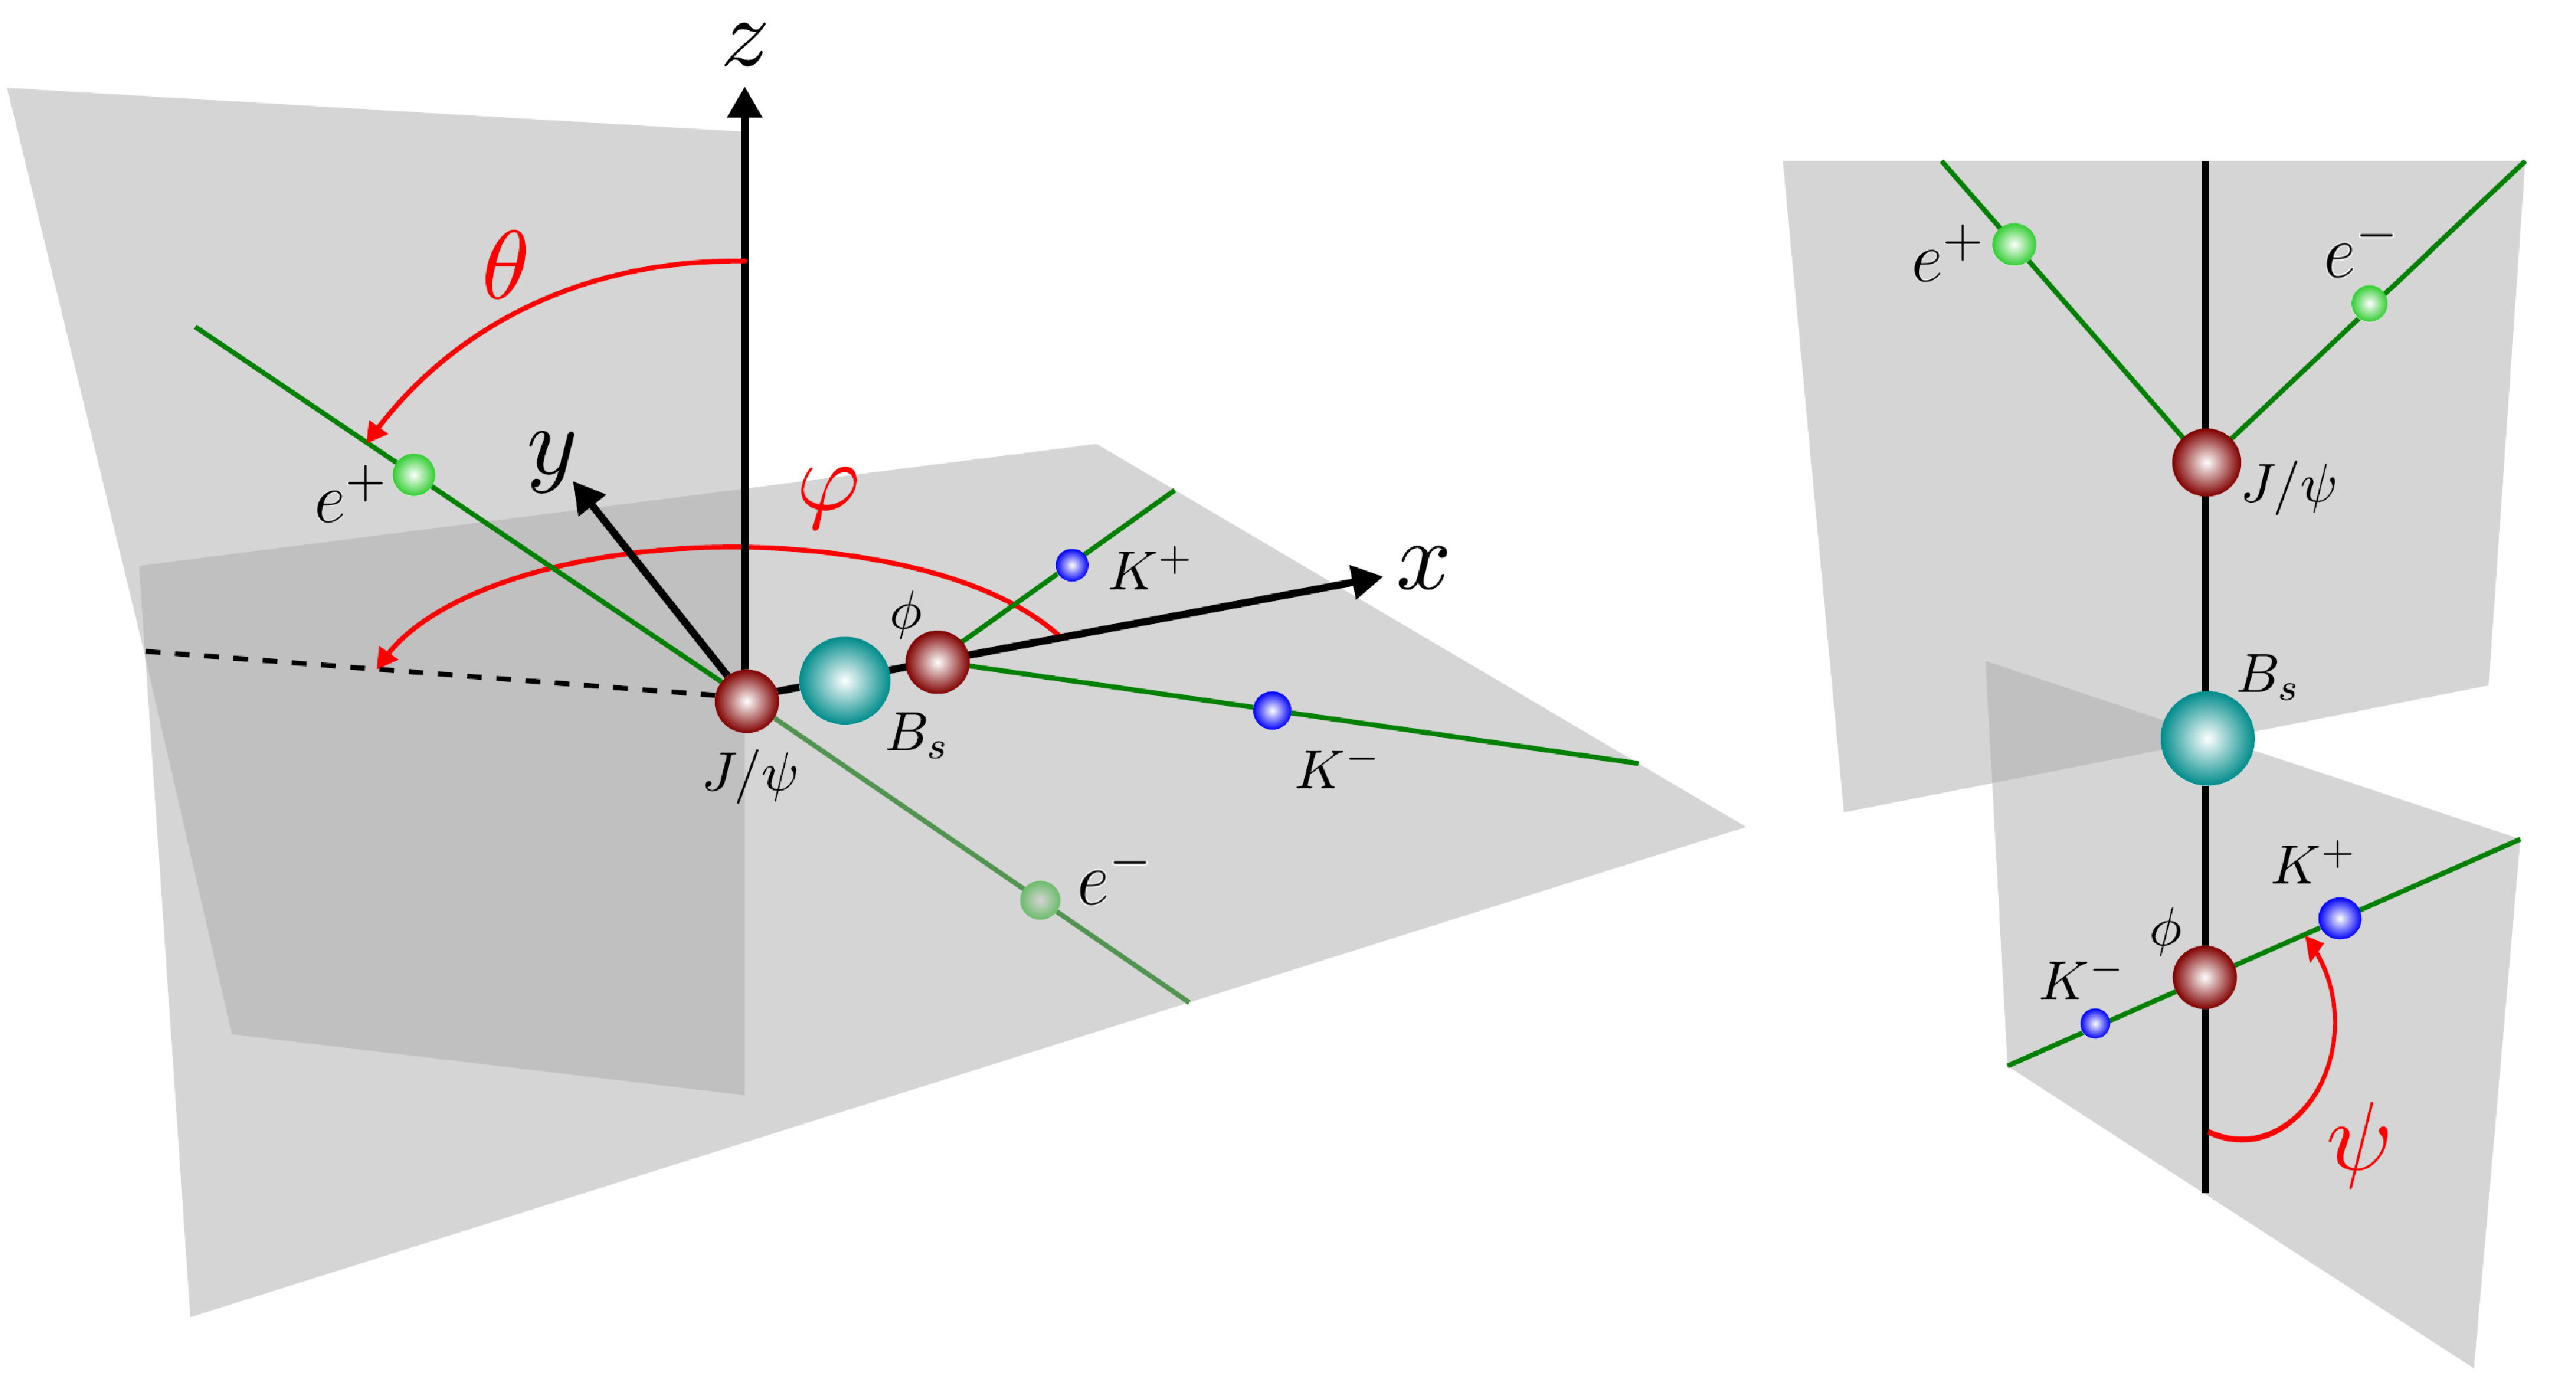
\includegraphics[width=0.8\linewidth]{Phenomenology/Angles_ee.pdf}
  \end{center}
  \caption{
   The angle definitions: $\theta$ is the angle formed by the positive lepton ($\ep$) and the $z$ axis, in the $\jpsi$ rest frame. The angle $\varphi$ is the azimuthal angle of $\ep$ in the same frame. In the $\phi$ meson rest frame, $\psi$ is the angle between $\vec{p}(\Kp)$ and $-\vec{p}(\jpsi)$. The definitions are the same for both $\Bs$ or a $\Bsb$ decays.   
}
  \label{fig:Phen:Angles}
\end{figure}
\clearpage


\section{Data samples, event reconstruction, selection and trigger}\label{sec:Data}
\subsection{Data samples}

The candidates of $\Bs\to\jpsi(\epem)\phi$ used in this analysis are selected from the data sample taken in 2011 at $\sqs$ = 7~$\tev$ and 2012 at $\sqs$ = 8~$\tev$. They are reconstructed with version 14 of the reconstruction software (Reco14). The 2011 data are stripped with version 21r1 (Stripping21r1-Merging-DV-v36r1), while the 2012 are stripped with 21 (Stripping21-Merging-DV-v36r1). In both cases, we use the Radiative stream and the {\tt StrippingBs2JpsieePhiDetachedLine}. 
The tuples are made on the GRID using $\davinci$ v37r2p4 with the track momentum scale calibration applied. Further processing is performed offline\footnote{Details of the code can be found in Appendix~\ref{sec:app:AnaCode}.} including application of the selection cuts, selection of single candidate for events with multiple ones, as well as calculation of the sWeights, the procedure for which is described in Sec.~\ref{sec:BsFit}. The integrated luminosity is 0.9875~$\invfb$ in 2011 and 2.0399~$\invfb$ in 2012.

\subsection{MC samples}\label{subsec:MC}

 The Monte Carlo (MC) samples are produced with Sim08 and listed in Table~\ref{tab:MC}. For each event type, half of the sample is produced with $\pythia$6, half with $\pythia$8, each of them being split equally into "magnet up" and "magnet down". The decays are preformed with $\evtgen$ and $\photos$++. The stripping is in "flagging mode", the reconstruction is "Reco14a", no prescale and no spillover are applied. For 2011-like MC samples, the trigger is simulated with $\moore$~v12r8g3 and TCK~0x40760037. For 2012 MC samples, the trigger is simulated with $\moore$~v14r8p1 and TCK~0x409f0045. The main physics parameters used in the simulation are summarized in Table~\ref{tab:MCparam}. A track level smearing has been applied to the simulated events to match the momentum resolution of the data.
   \begin{table}[hbt]
  \caption{
    Monte Carlo samples used in the analysis. All samples are produced with Sim08. The number of events quoted is the sum of $\pythia$6(MagUp)+$\pythia$6(MagDown)+$\pythia$8(MagUp)+$\pythia$8(MagDown), for 2011 plus 2012.}
    \small{
\begin{center}\begin{tabular}{lccc}
    \hline
    Decay Channel                         &  & Event type & Tot. number of events       \\ 
    \hline
    Bs$\_$Jpsiphi,ee=CPV,update2012,DecProdCut   &  & 13154001 &  20M\\
    incl$\_$Jpsi,ee=DecProdCut &  & 24152001  & 20M \\
    Bu$\_$JpsiX,ee=JpsiInAcc & &  12952000 & 13.4M \\
    Bd$\_$JpsiX,ee=JpsiInAcc & &  11453001 & 11.6M \\
    Bs$\_$JpsiX,ee=JpsiInAcc & &  13454001 & 11M \\
    Lb$\_$JpsiX,ee=JpsiInAcc & &  15454101 & 11.4M \\
    Lb$\_$JpsipK,ee=phsp,DecProdCut & &  15154001 & 10M \\
    Lb$\_$Jpsippi,ee=phsp,DecProdCut & &  15154021 & 10M \\
    \hline
  \end{tabular}\end{center}
  }
\label{tab:MC}
\end{table}

 \begin{table}[hbt]
  \caption{
    Decay model parameters for the Sim08 MC signal sample used in this analysis. The parameter values are based on those reported in Ref.~\cite{Aaij:2013oba}.}
    \small{
\begin{center}\begin{tabular}{cc}
    \hline
    Parameter                         &  Value       \\ 
    \hline
    $\dms$   &  17.8~$\invps$\\
    $\DGs$  & 0.0917~$\invps$ \\
    $\Gs$   & 0.6653~$\invps$ \\
    $\phis$ & 0.07~$\rad$ \\
    $|A_{0}(0)|^{2}$ & 0.722 \\
    $|A_{\parallel}(0)|^{2}$ & 0.480 \\
    $|A_{\perp}(0)|^{2}$ & 0.499 \\
    $\delta_{\parallel}-\delta_{0}$ & 3.30~$\rad$\\
    $\delta_{\perp}-\delta_{0}$ & 3.07~$\rad$\\
    \hline
  \end{tabular}\end{center}
  }
\label{tab:MCparam}
\end{table}
 
 \subsection{Event Selection}\label{subsec:EvtSel}
 
 For the events selected by the stripping line, first the $\jpsi\to\epem$ decay is reconstructed, then the $\phi\to\Kp\Km$ decay and finally the $\Bs\to\jpsi\phi$ is looked for.
 Table~\ref{tab:Selection} summarizes the requirements in the stripping line as well as additional preselection requirements that are applied.

  \begin{table}[hbt]
  \caption{
    Selection criteria for $\BsToJPsiPhi$ candidates in Stripping21{r1} and preselection. 
}
    \small{
\begin{center} \begin{tabular}{|c|c|c|c|}
    \hline
 Decay mode & Cut parameter & Stripping & Preselection  \\
  \hline
 $\jpsi\to\epem$ & $\Delta ln\mathcal{L}_{e\pi}$ & $>$0 & - \\
 & $\chisq_{\text{track}}$/ndf($e$) & $<$5 & $<$4 \\
 & $\chisqip(e)$ & - & $>$0 \\
 & $\pt(e)$ & $>$500~$\mevc$ & - \\
 & $\chisqvtxndf(\jpsi$) & $<$15 & - \\
 & $\pt(\jpsi)$ & - & $>$400~$\mevc$ \\
 & $m(\jpsi)$ & $\in$[2500, 3300]~$\mevcc$ & - \\
 \hline
  $\phi\to\Kp\Km$ & $\Delta ln\mathcal{L}_{K\pi}$ & - & $>$0 \\
  & $\chisq_{\text{track}}$/ndf($K$) & - & $<$4 \\
  & $\pt(K)$ & - & $>$200~$\mevc$ \\
  & $p(K)$ & - & $>$3000~$\mevc$ \\
  & GhostProb$_{\text{track}}(K)$ & - & $<$0.5 \\
 & $\pt(\phi)$ & $>$1000~$\mevc$ & - \\
 & $\chisqvtxndf(\phi$) & $<$15 & $<$9 \\
 & $m(\Kp\Km)$ & $\in$[990, 1050]~$\mevcc$ & - \\
 \hline
  $\Bs\to\jpsi\phi$ & $m(\Bs)$ & $\in$[4500, 6000]~$\mevcc$ & $\in$[4600, 6000]~$\mevcc$ \\
 & $\chisqvtxndf(\Bs$) & $<$10 & - \\
 & $\chisqip(\Bs$) & - & $<$20 \\
 & $t$ & $>$0.3~$\ps$ & - \\
 \hline
    \end{tabular}\end{center}
  }
\label{tab:Selection}
\end{table}

\subsection{Trigger}\label{subsec:Trigger}

The stripping and final event selection are chosen in a way to not affect the decay time acceptance. The trigger is the only source of the time dependent inefficiency is the trigger. For this reason the trigger lines are divided into two categories: a decay time unbiased and biased trigger lines. The trigger categories are defined as follows:
 \begin{enumerate}
  \item Unbiased: {\tt L0ElectronDecision$\_$TOS} or {\tt L0HadronDecision$\_$TOS}
  \item Biased: ({\tt Hlt1TrackAllL0Decision$\_$TOS} and ({\tt Hlt2Topo(2,3,4)BodyBBDTDecision$\_$TOS} or {\tt Hlt2TopoE(2,3,4)BodyBBDTDecision$\_$TOS})) or {\tt Hlt2IncPhiDecision$\_$TOS} 
 \end{enumerate}

 The unbiased triggers correspond to approximately 72$\%$ and 81$\%$ of the selected events in data and MC, respectively, as shown in Fig.~\ref{fig:TimeTrigger}.
 \begin{figure}[hbt]
  \begin{center}
    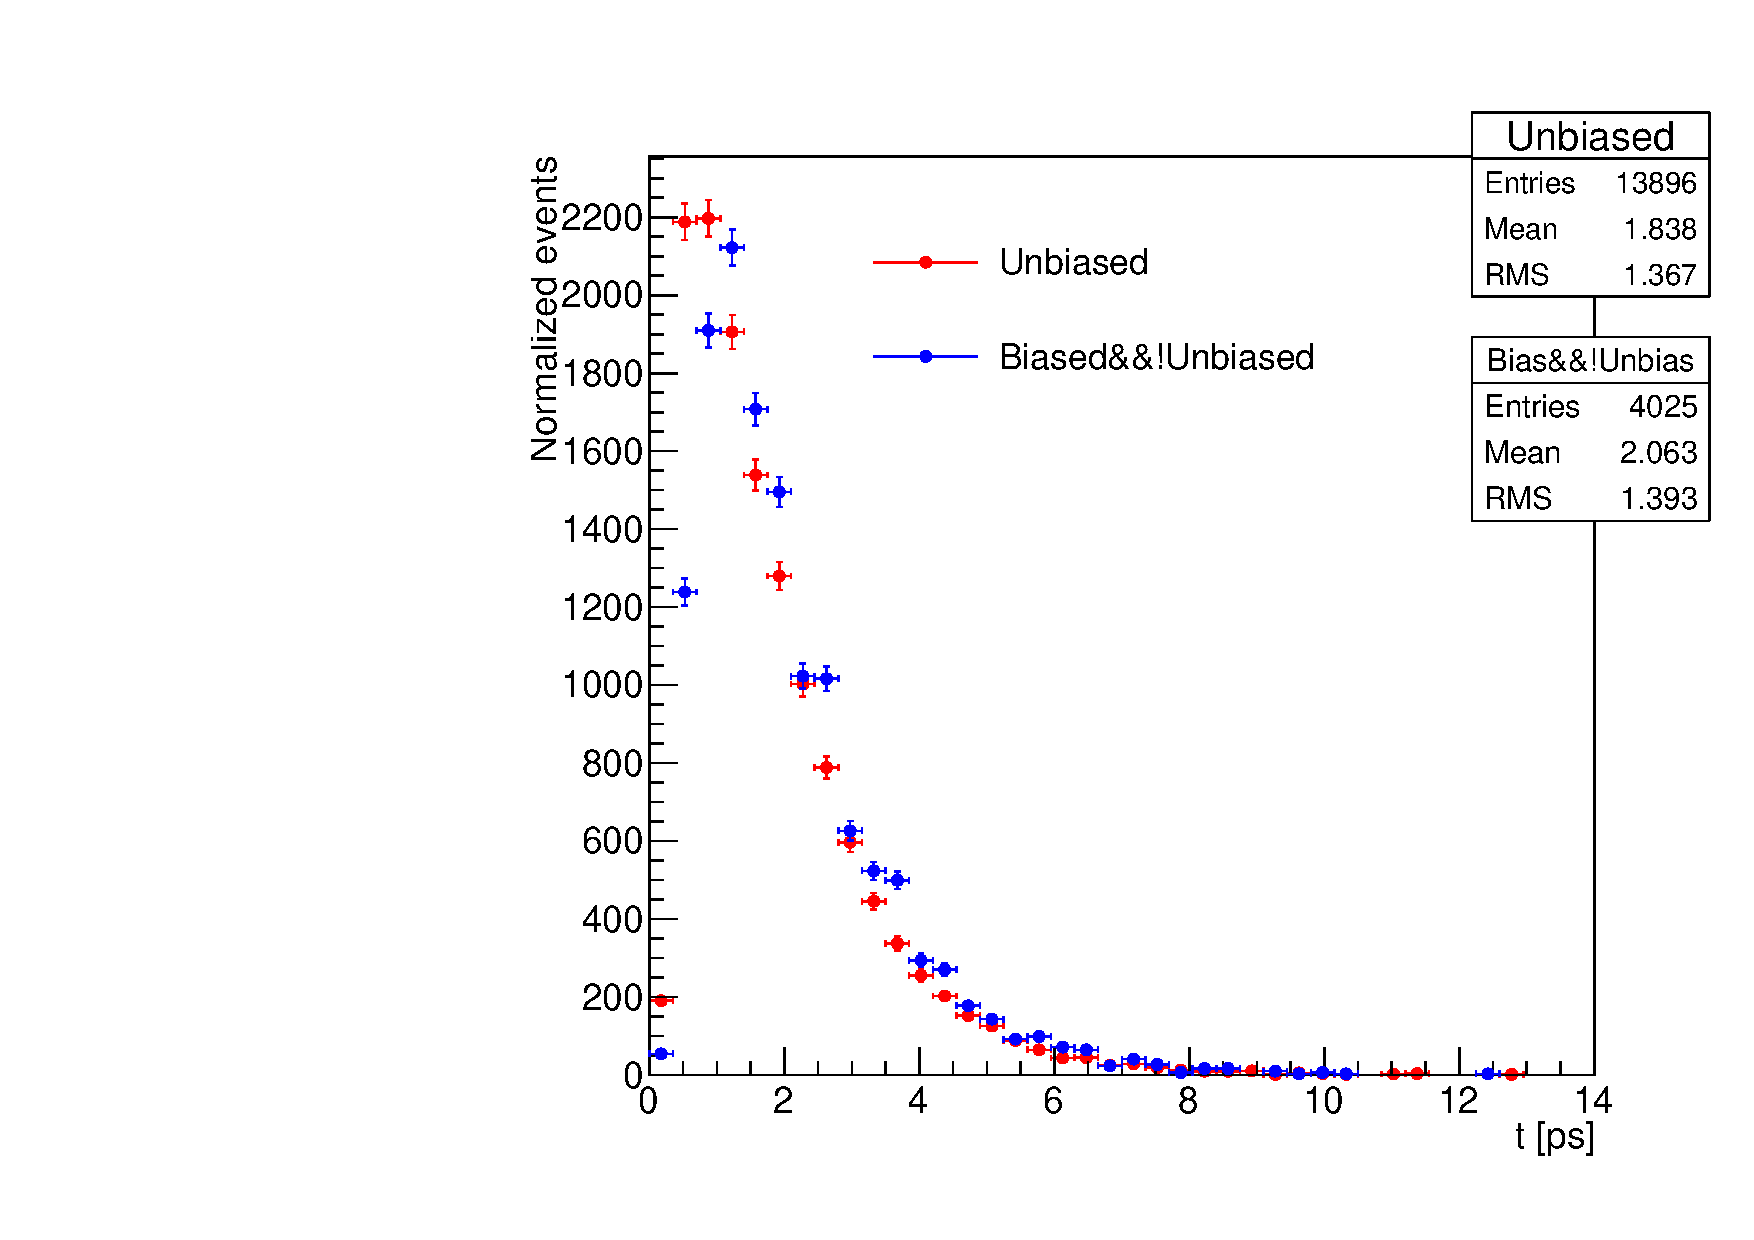
\includegraphics[width=0.48\linewidth]{Trigger/RDfull.pdf}\put(-115,-4){(a)}
    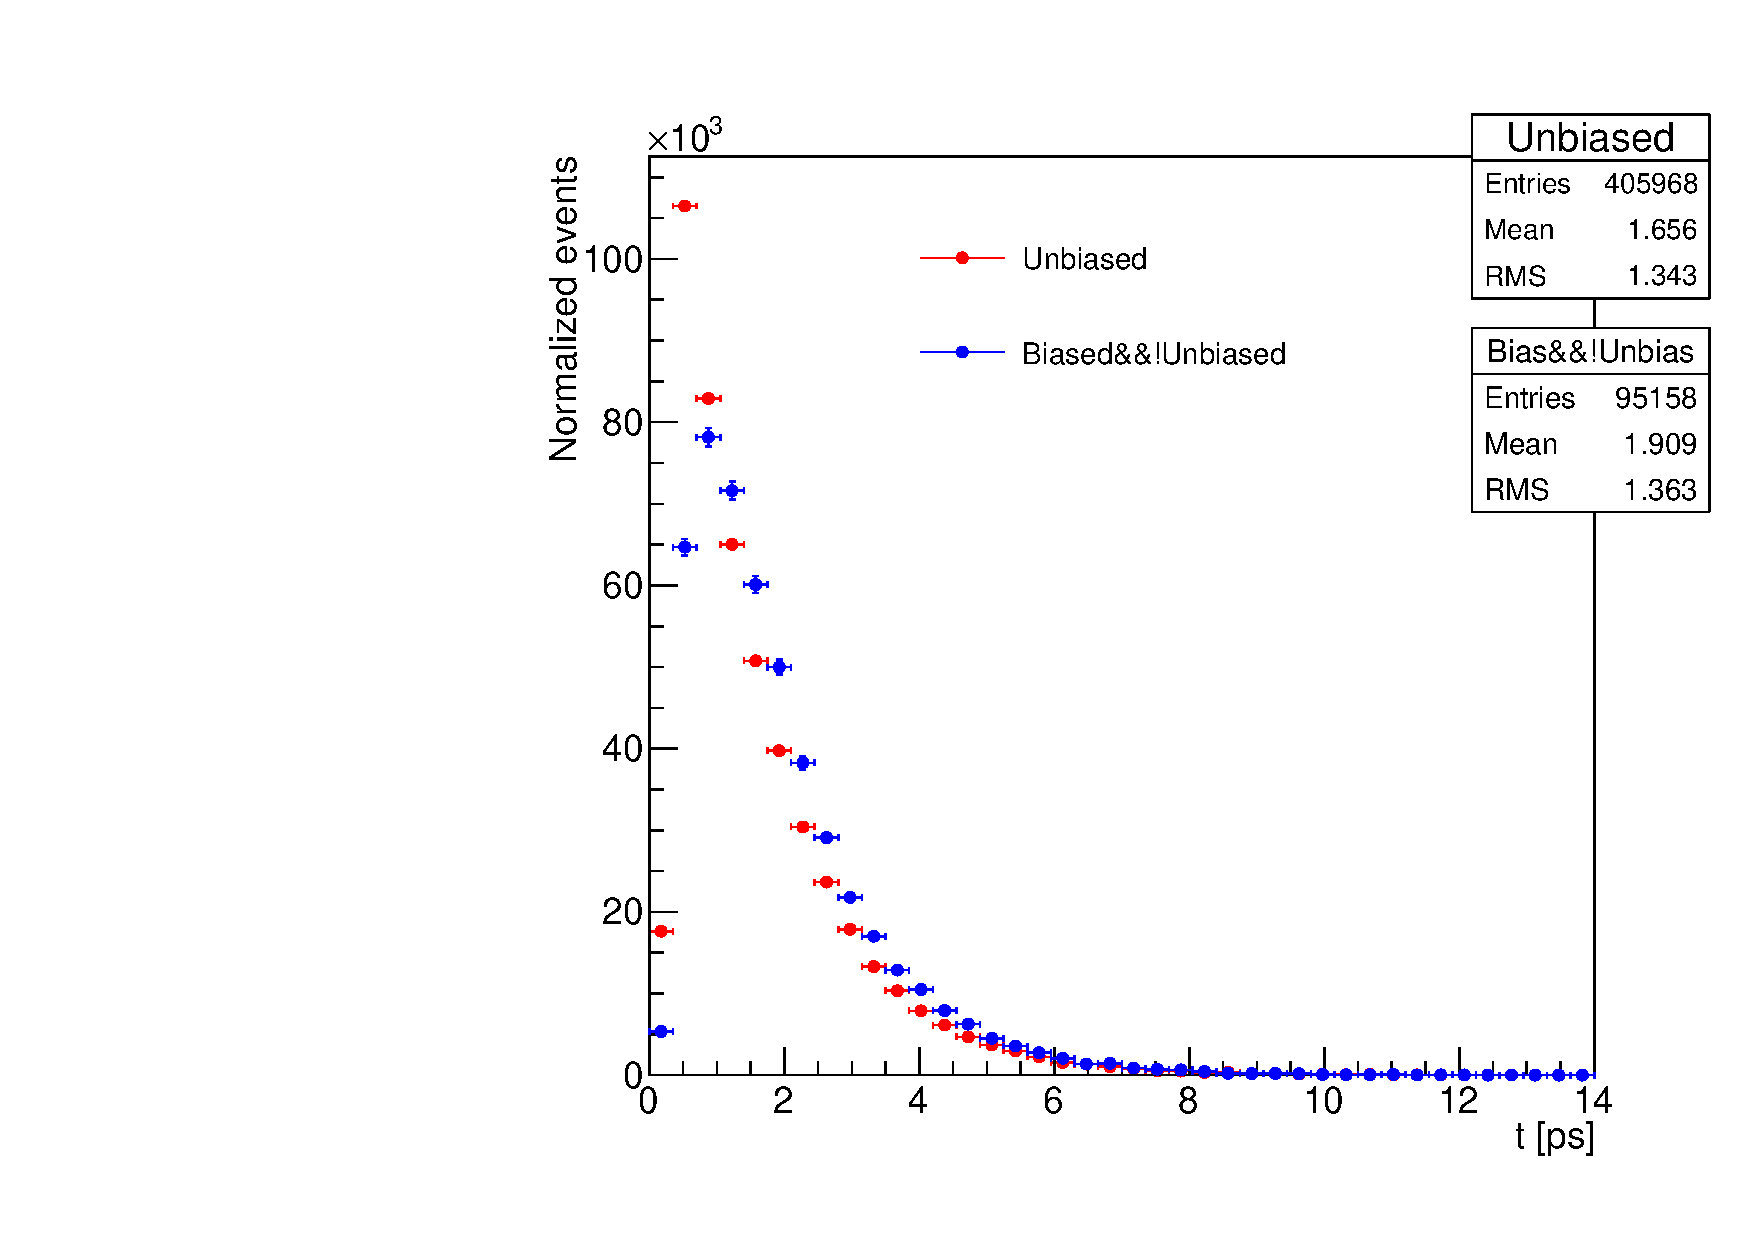
\includegraphics[width=0.48\linewidth]{Trigger/MCfull.pdf}\put(-115,-4){(b)}
  \end{center}
  \caption{
   The decay time distribution of the events which are triggered by the unbiased triggers (red) and by the biased ones but not by unbiased (blue) for data (a) and MC (b).  
}
  \label{fig:TimeTrigger}
\end{figure}
 
 The procedure to derive the decay time dependent efficiencies of these trigger categories are described in Sec.~\ref{sec:TimeAcc}. 
 
 \subsection{Monte Carlo reweighting}\label{subsec:MCreweight}
 While there is in general a good agreement between data and MC for the samples used in this analysis, a significant difference exists in the event occupancy being largely under-estimated in the simulated data. The occupancy correlates to the invariant mass shape of the signal as the correction of the electron momenta for the bremsstrahlung photons emitted before the magnet depends on proper measurement of particles energies in the electromagnetic calorimeter (ECAL). Therefore, it is important to property include this effect in the MC. A way to accommodate data and MC difference is to use the scintillating pad detector (SPD) hits multiplicity distribution, which is highly correlated to the event occupancy. Therefore, a reweighting of the simulated events is applied in order to match their SPD multiplicity distribution to the LHCb data. The procedure used for this analysis is the same as described in Ref.~\cite{Borsato:2014-009}.
 
The discrepancy in the SPD hit multiplicity between data and MC is presented in Fig.~\ref{fig:nSPDHits}(a). The reweighting is performed separately for 2011 and 2012 as the average number of interactions per bunch crossing was different in the two years. The weights, which are applied to the simulation, are shown in Fig.~\ref{fig:nSPDHits}(b). Comparison between data and MC before and after corrections are applied and they are shown in Appendix~\ref{sec:app:DataMC}.  

\begin{figure}[htb]
  \begin{center}
    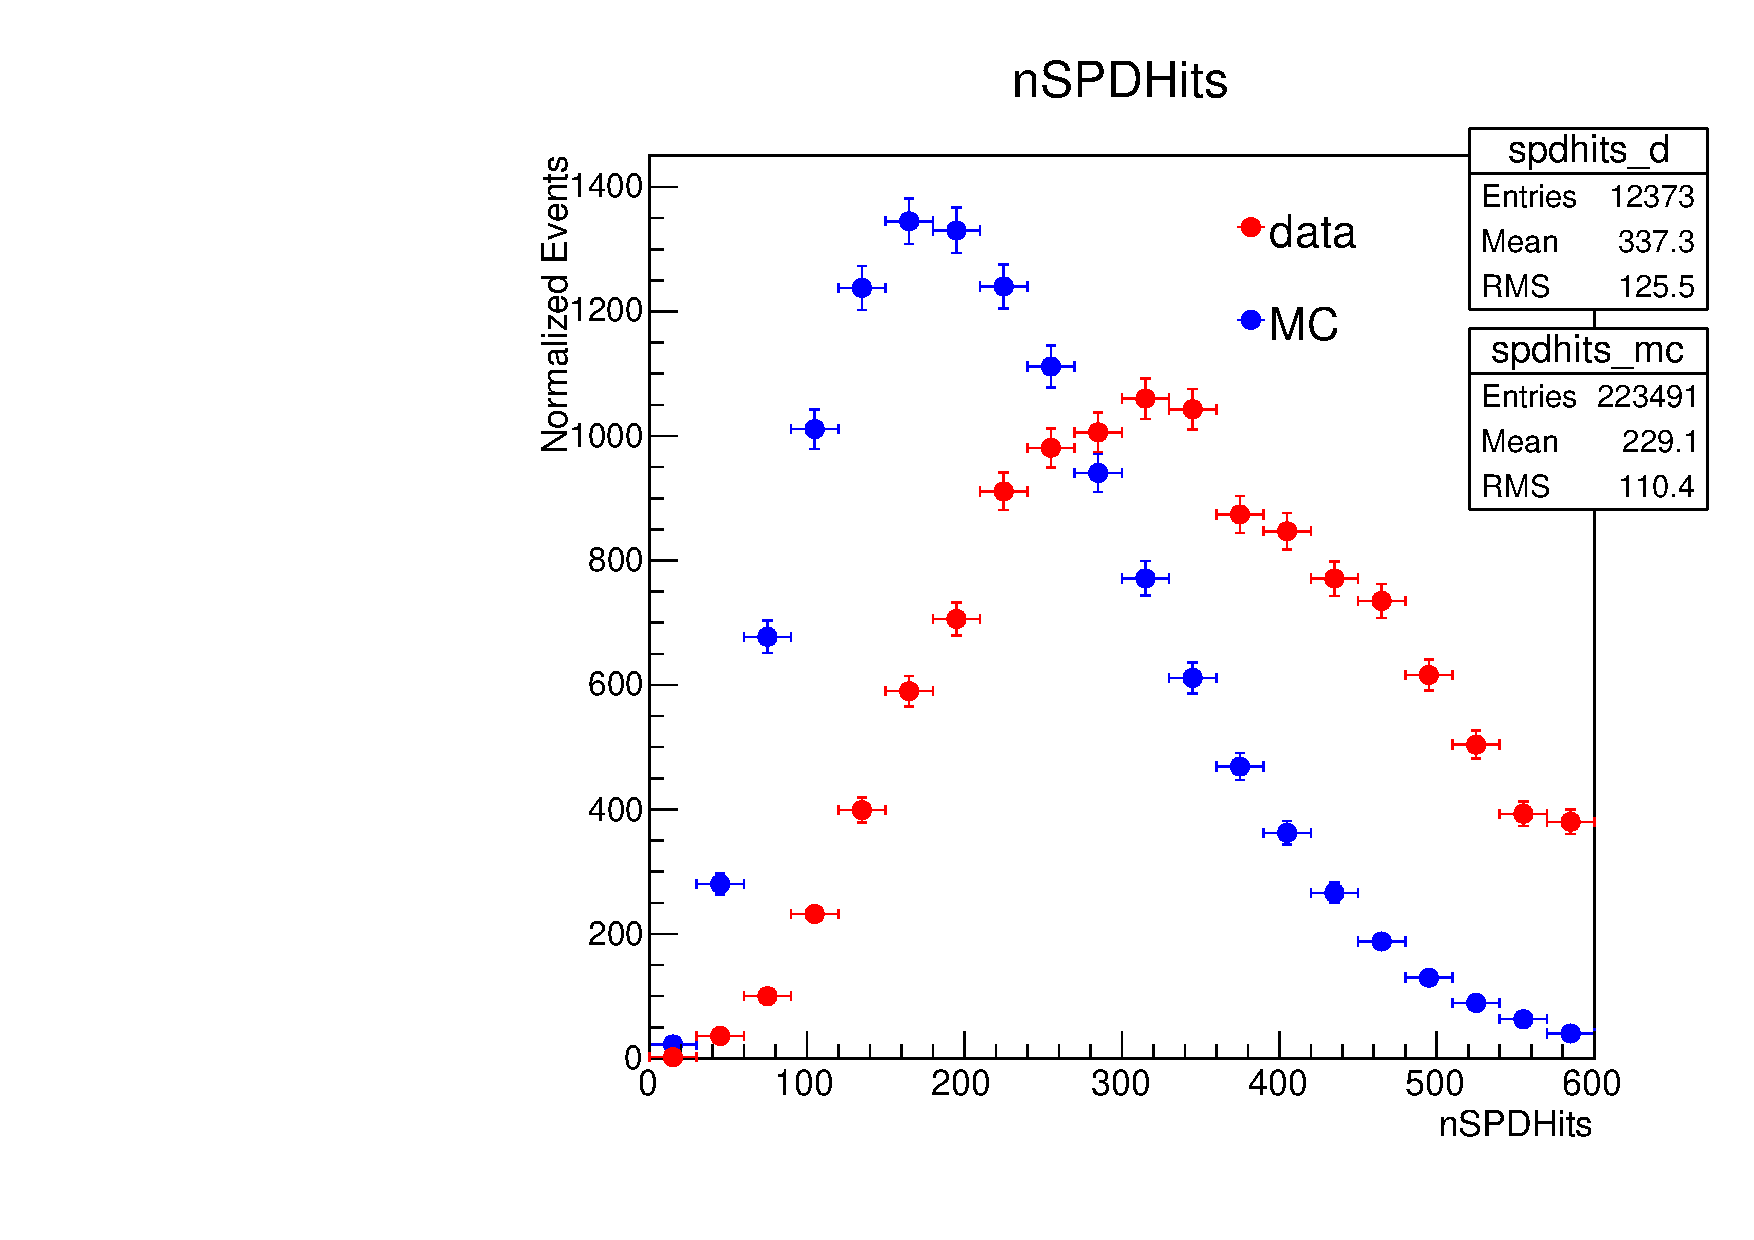
\includegraphics[width=0.48\linewidth]{MC/SPDHits_RD_MC12_BDT1_BDT2_sWeight.pdf}\put(-115,-4){(a)}
    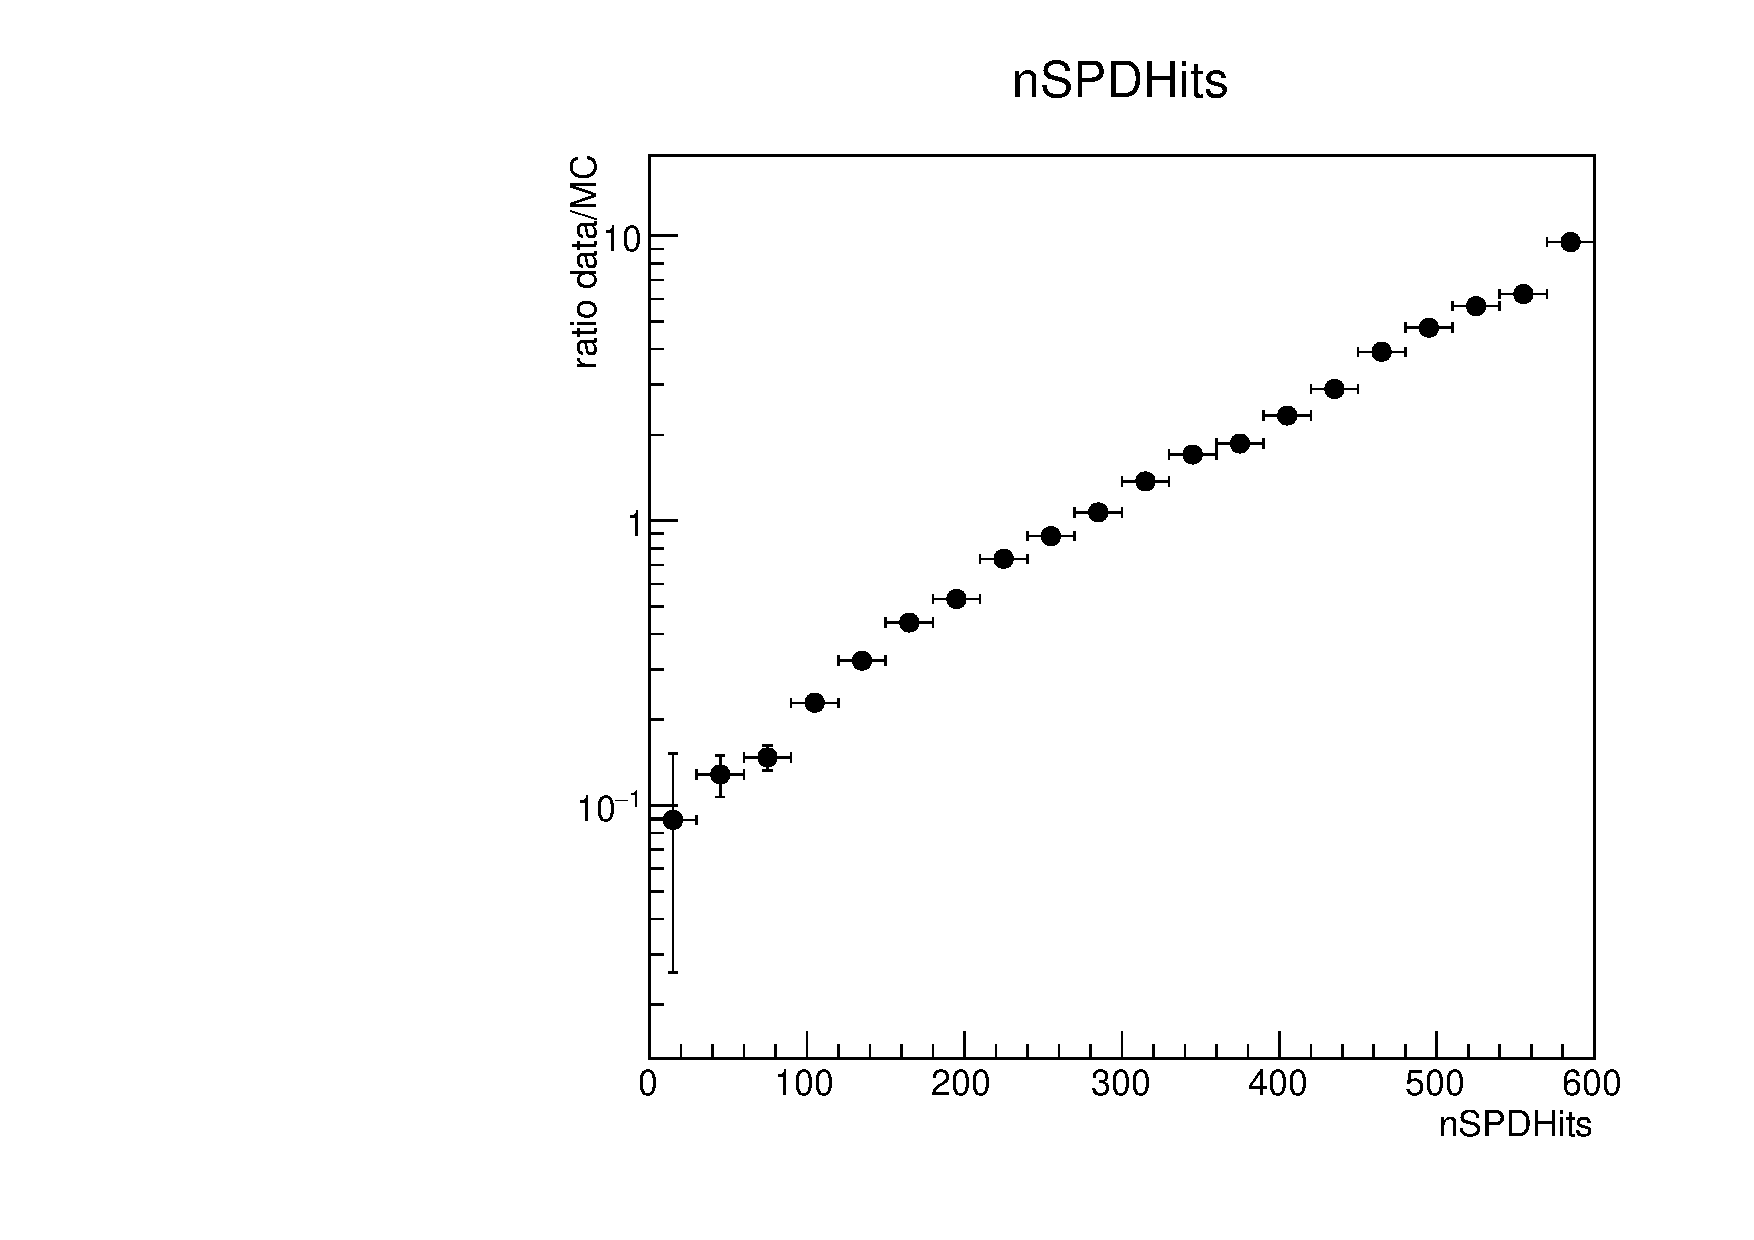
\includegraphics[width=0.48\linewidth]{MC/SPDHits_RD_MC12_BDT1_BDT2_sWeight_ratio.pdf}\put(-115,-4){(b)}
  \end{center}
  \caption{
   (a) The distribution of the number of hits in the SPD for $\Bs\to\jpsi(e^{+}e^{-})\phi$ data and MC in 2012. (b) The ratio between data and MC distributions in depends on the number of hits on the SPD. The ratio distribution is in logarithmic scale.
}
  \label{fig:nSPDHits}
\end{figure}


\subsubsection{Correction of the PID response}\label{subsubsec:PIDCalib}

The PID response is known to be not well simulated in the LHCb MC. Therefore, instead of applying the cut on the PID variables calculated in the MC, events are reweighted using PID efficiency tables. The {\tt Urania/PIDCalib} package version {\tt v4r0} is used to build PID efficiency tables for all final state particle types, $K^{\pm}$ and $e^{\pm}$. The PID efficiencies are calculated in bins of $\eta$, $p_{T}$ and number of tracks in the event. For each MC event the total PID efficiency is calculated and used to weight the event (Fig.~\ref{fig:PIDCalib}). 
\begin{figure}[htb]
  \begin{center}
    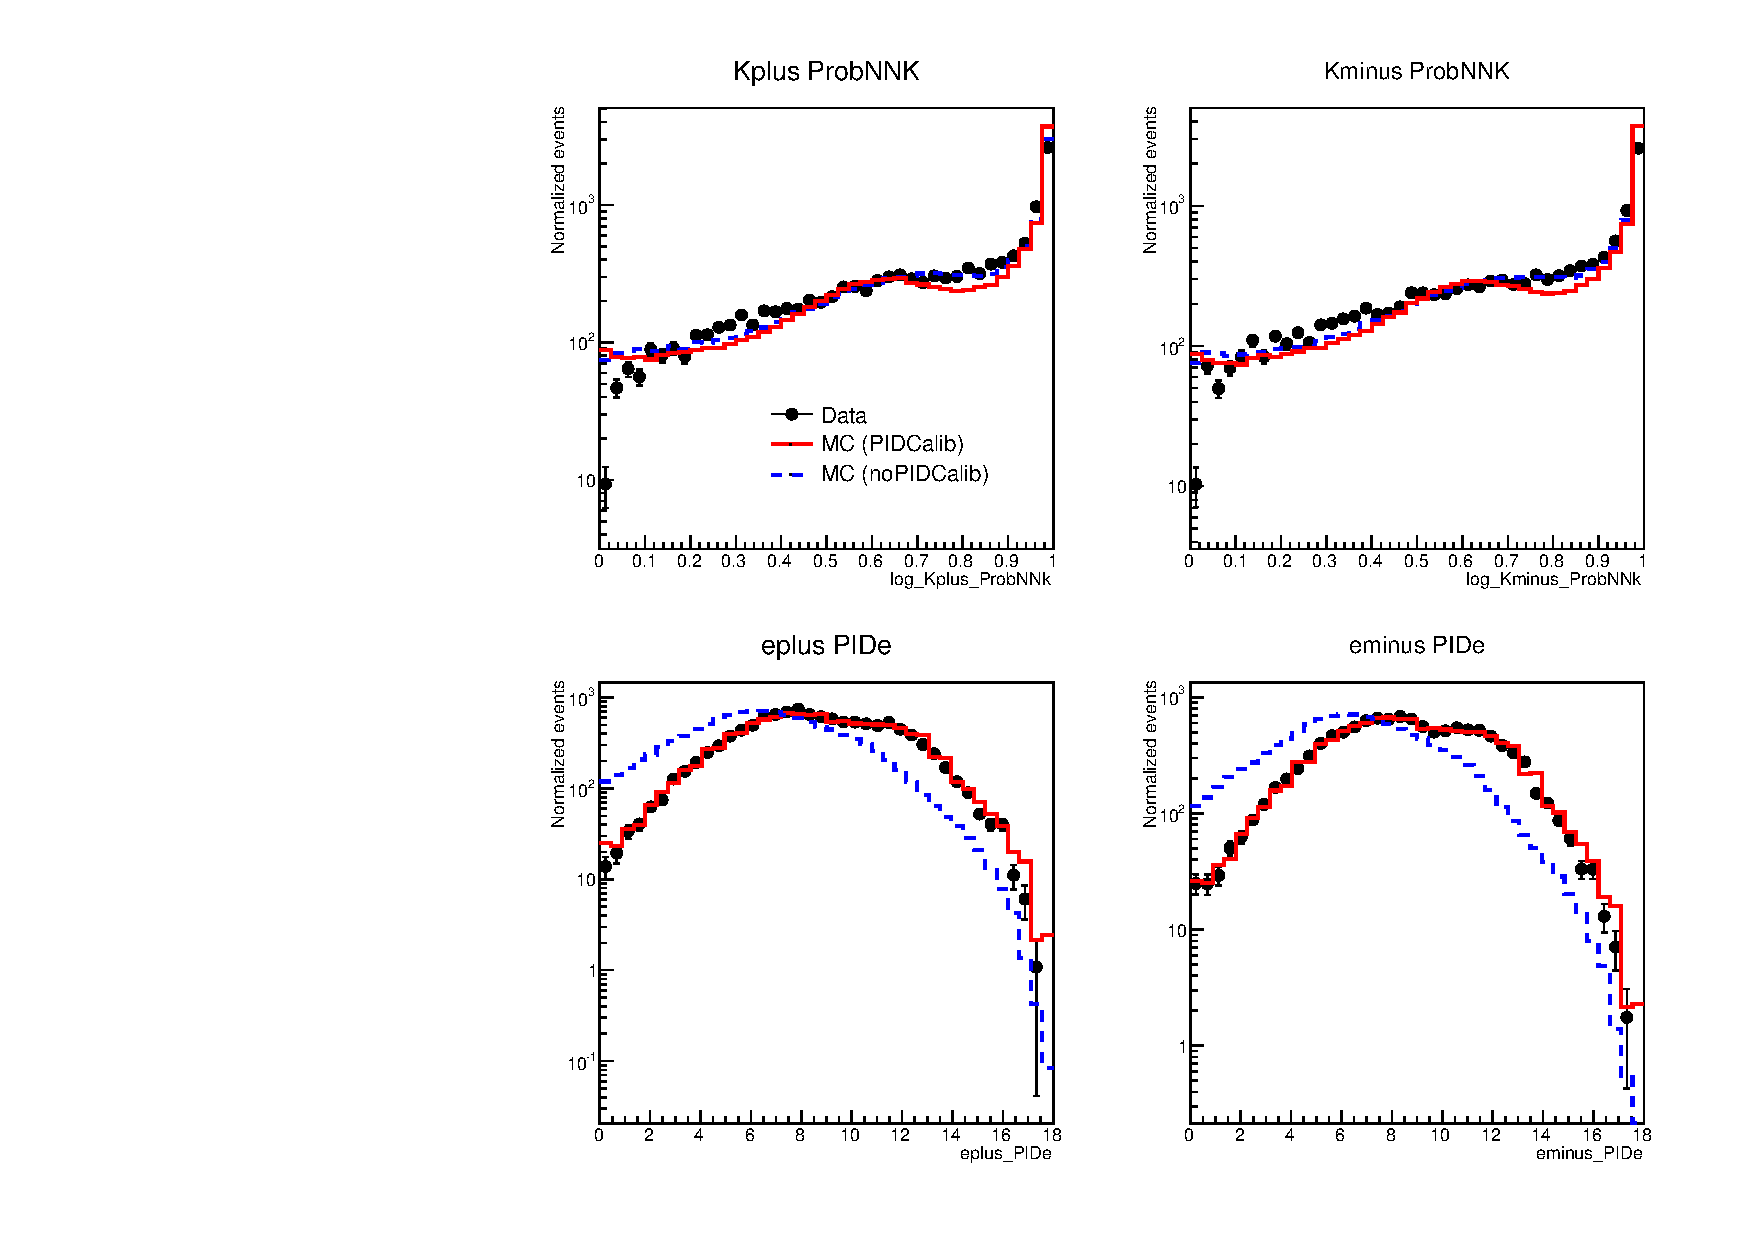
\includegraphics[width=0.8\linewidth]{Data_MC/Data_MC_PIDCalib.pdf}
  \end{center}
  \caption{
   The ProbNNK($\Kpm$) and PIDe($\epm$) distributions for $\Bs\to\jpsi(e^{+}e^{-})\phi$ in: data (black points), MC (blue dashed line) and {\tt PIDCalib} simulated data (red solid line). All distributions are in logarithmic scale.
}
  \label{fig:PIDCalib}
\end{figure}

After applying {\tt PIDCalib} algorithm the electron PIDe values for MC are in agreement with PID values for data. However, the opposite distributions obtained for ProbNN values of kaons. The kaon ProbNNK distributions for data are comparable with simulation without {\tt PIDCalib}. Thus the corrected PIDe($\epm$) and non-corrected ProbNNK($\Kpm$) variables are used in the further selection (see Sec.~\ref{subsec:BDT}).   

 \subsection{Boosted Decision Tree}\label{subsec:BDT}
  After stripping and preselection criteria (Table~\ref{tab:Selection}), the amount of background events remaining in the sample is considerable and the additional selection is required. The Boosted Decision Tree (BDT)~\cite{Hocker:2007ht} are chosen to further discriminate the signal candidates from the background. In order to have a good agreement between data and simulation, a set of kinematic variables is chosen for the BDT discriminator. In particular 12 variables are taken into consideration:
  \begin{itemize}
   \item $\pt(\jpsi)$ - the transverse momentum of the $\jpsi$ meson;
   \item $\pt(\phi)$ - the transverse momentum of the $\phi$ meson;
   \item IP$(\Bs)$ - the impact parameter of the reconstructed $\Bs$ meson with respect to the primary vertex;
   \item $\chisq_{\text{FD}}(\Bs)$ of the measured flight distance of the $\Bs$ meson;
   \item $\chisqip$ of the impact parameter of the electron and positron;
   \item $\chisqvtxndf$ of the reconstructed secondary vertex;
   \item PIDe - the difference of log-likelihood between electron and pion hypothesis for the electron and positron. In case of MC the PIDe is reweighted using {\tt PIDCalib} tool (Sec.~\ref{subsubsec:PIDCalib}) and is called PIDe$_{\text{corr}}$;
   \item ProbNNK - Neural Net (NN) log-likelihood of the kaon hypothesis for the kaons;
   \item $\chisq_{\text{DTF}}$ of the reconstructed $\Bs$ meson. 
  \end{itemize}

  The training of the BDT is done using the following samples:
  \begin{itemize}
   \item Signal: the $\Bs\to\jpsi\phi$ simulated sample is used as signal model. This sample is required to pass exactly the same stripping and preselection criteria and, furthermore, the MC truth information is used to require that the reconstructed candidate matches with the generated decay.
   \item Background: a wrong sign $\Bs\to\jpsi\phi$ data sample is used. In particular $\Bs\to\jpsi(\ep\ep)\phi(\Kp\Kp)$,  $\Bs\to\jpsi(\ep\ep)\phi(\Km\Km)$, $\Bs\to\jpsi(\en\en)\phi(\Kp\Kp)$, $\Bs\to\jpsi(\en\en)\phi(\Km\Km)$, $\Bs\to\jpsi(\ep\ep)\phi(\Kp\Km)$, $\Bs\to\jpsi(\en\en)\phi(\Kp\Km)$,  $\Bs\to\jpsi(\epem)\phi(\Kp\Kp)$ and $\Bs\to\jpsi(\epem)\phi(\Km\Km)$ events make the background sample. Also these events are required to pass all the selection steps.
  \end{itemize}
   
   The choice to use a wrong sign $\Bs\to\jpsi\phi$ data sample instead of data events taken from the sidebands of the $\Bs$ mass distribution is motivated by the fact that in this way the signal and background samples are more homogeneous. The sideband events from data ($M(\Bs)<5050$ MeV and $M(\Bs)>5550$ MeV) have also been considered to simulate the background events in the BDT training. A worse agreement between sidebands data and simulation is observed in the BDT performance description. 

  The ranking of variable importance used to train the BDT is shown in Table~\ref{tab:RankingBDT}. The BDT response is presented in Fig.~\ref{fig:BDTresponse}a. The further details on the BDT, including plots comparing the input variable distributions between signal and background, are prsented in  Appendix~\ref{sec:app:BDT}. 
   \begin{table}[hbt]
  \caption{
    The ranking of variable importance used in BDT selection.
}
    \small{
\begin{center} \begin{tabular}{ccc}
    \hline
   Rank&Variable & Importance  \\
    \hline
  1&log(ProbNNK)$(K^{+})$ & 1.149e-01 \\
  2&PIDe$(e^{-})_{\text{corr}}$ & 1.075e-01 \\
  3&log(ProbNNK)$(K^{-})$ & 1.066e-01 \\
  4&log$(\chi^{2}_{\text{IP}})(e^{-})$ & 9.723e-02 \\
  5&PIDe$(e^{+})_{\text{corr}}$ & 9.430e-02 \\
  6&log$(\chi^{2}_{\text{IP}})(e^{+})$ & 8.902e-02 \\
  7&$p_{T}(\phi)$ & 8.500e-02 \\
  8&IP$(B^{0}_{s})$ & 8.456e-02 \\
  9&$\chi^{2}_{\text{vtx}}(B^{0}_{s})$ & 7.939e-02 \\
  10&$p_{T}(J/\psi)$ & 7.595e-02 \\
  11&log$(\chi^{2}_{\text{DTF}})(B^{0}_{s})$ & 6.565e-02 \\
  12&$\chi^{2}_{\text{FD}}(B^{0}_{s})$ & 0.000e+00 \\
  \hline
    \end{tabular}\end{center}
  }
\label{tab:RankingBDT}
\end{table}

\begin{figure}[ht!]
  \begin{center}
    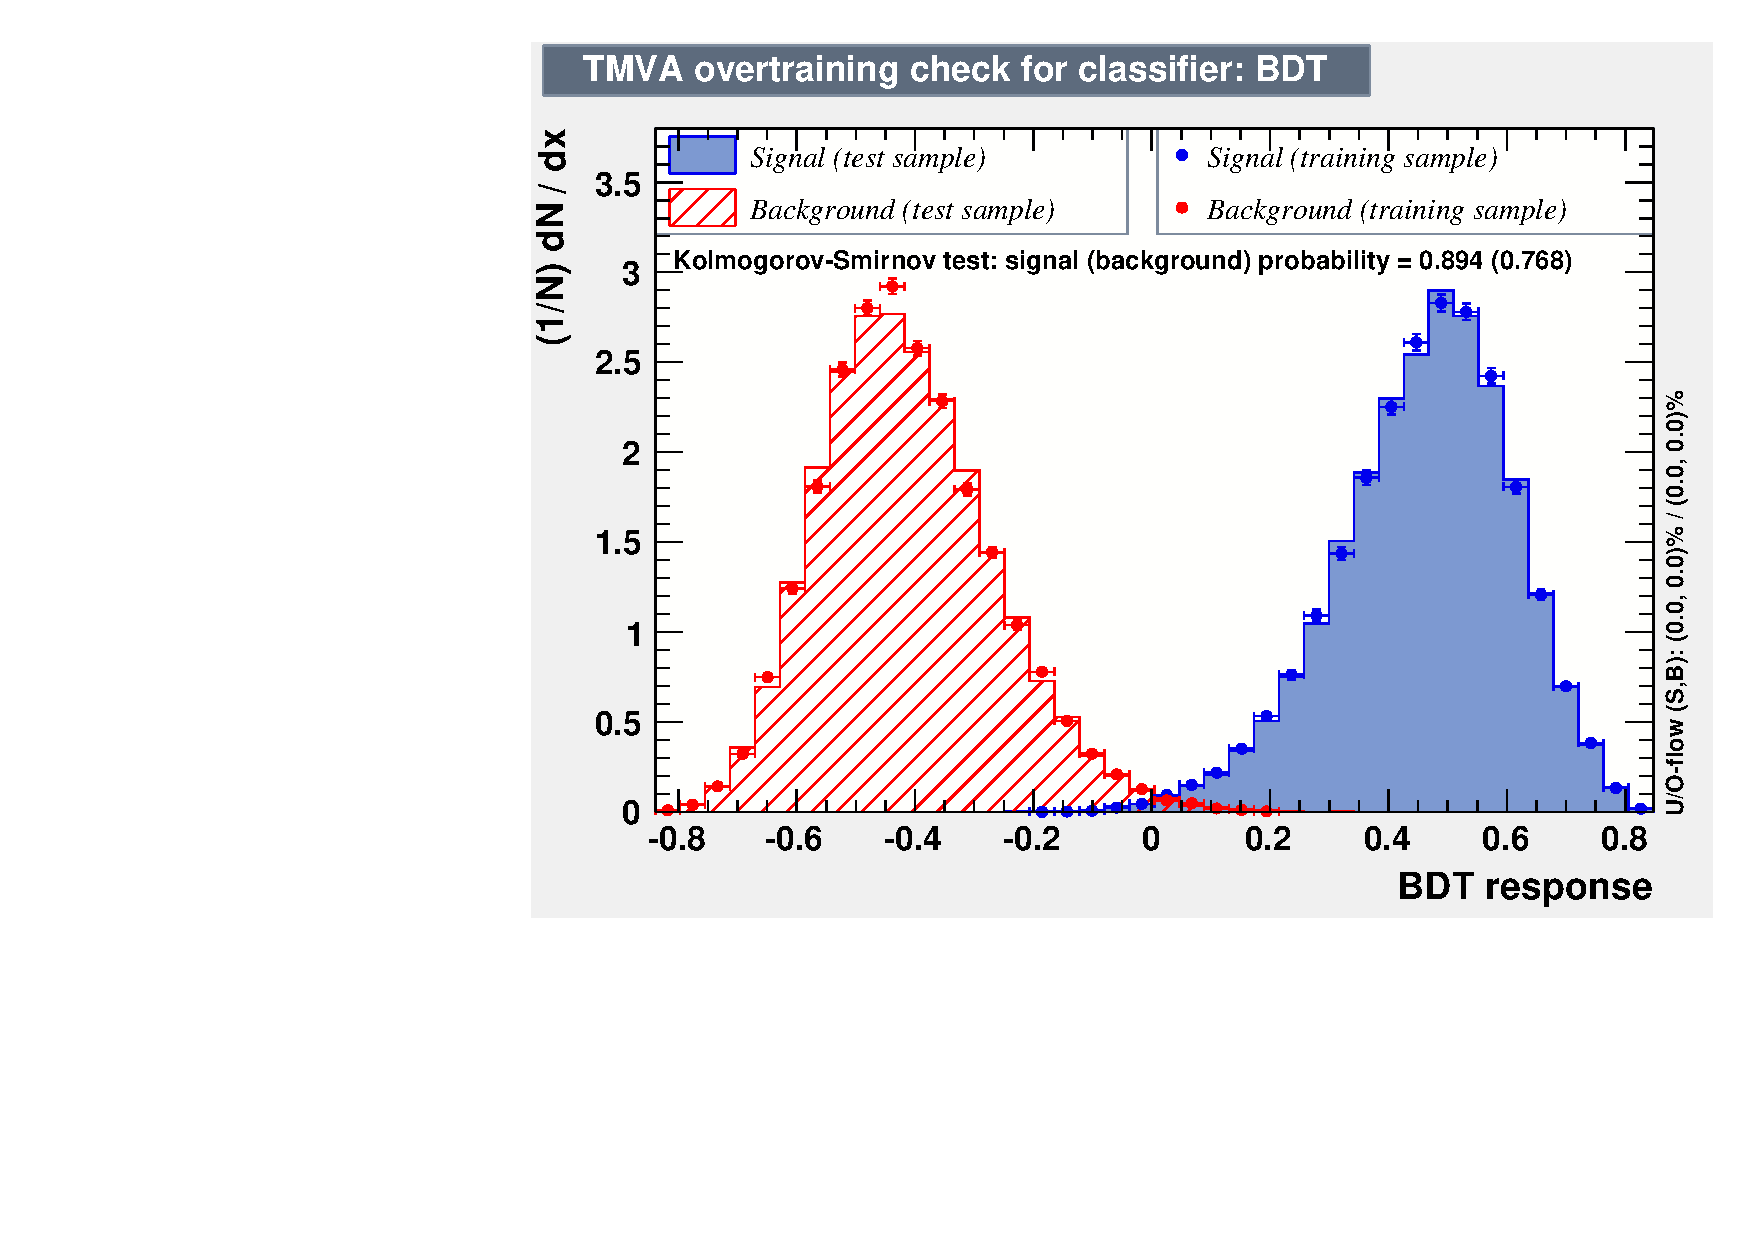
\includegraphics[width=0.49\linewidth]{BDT/BDT_response_bkgcat0_wSPDHits_trigger_RD12.pdf}\put(-115,-13){(a)}
    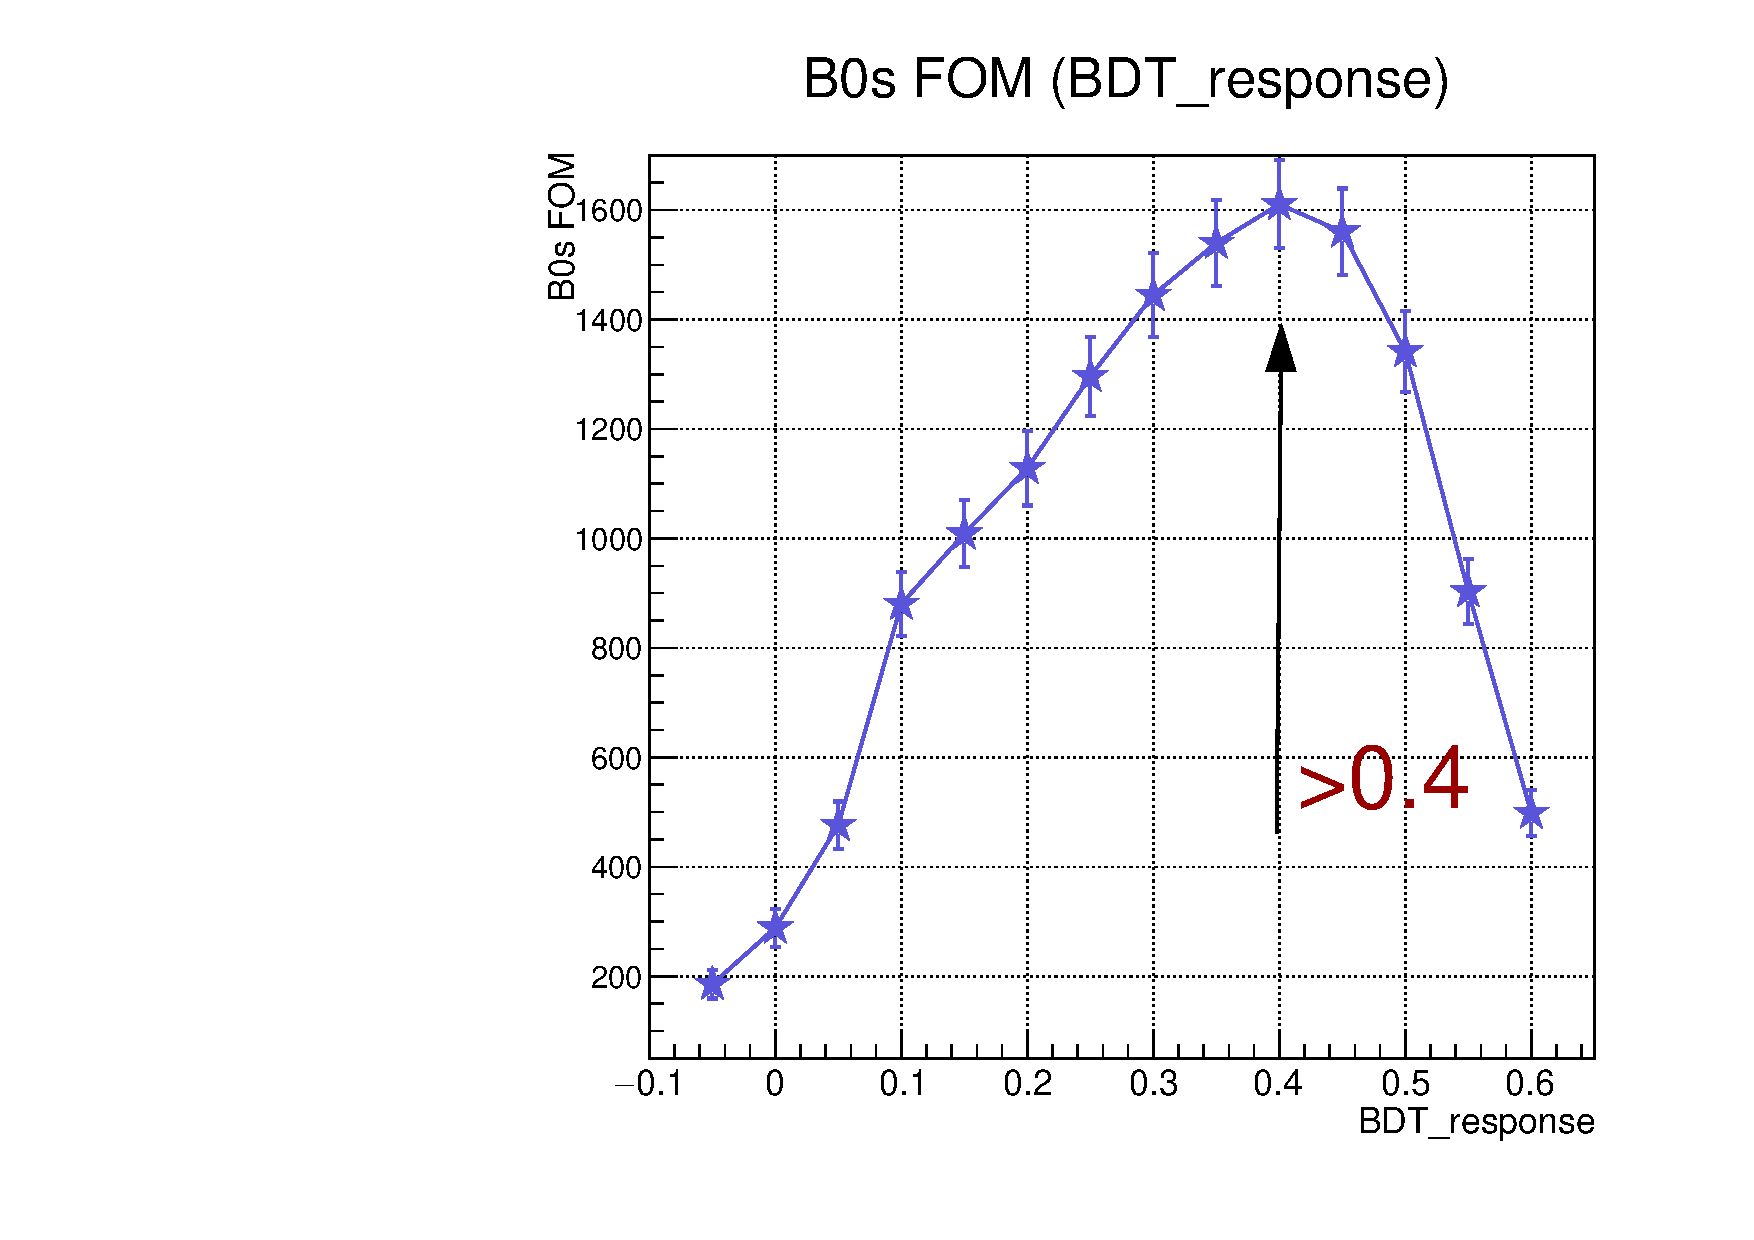
\includegraphics[width=0.41\linewidth]{BDT/FoM_BDT_response.pdf}\put(-115,-13){(b)}
  \end{center}
  \caption{
   (a) The distributions of the BDT classifier for $\Bs\to\jpsi\phi$ training samples. The signal is red hatched filled while the background is blue solid filled.  (b) The distribution of the FoM value vs. cut on the BDT response.  
}
  \label{fig:BDTresponse}
\end{figure}
  The BDT response is the combined vote of many individual decision trees. It can be used as a univariate discriminant to distinguish signal from background. To choose where to cut on the BDT response we use a figure of merit (FoM) value (Eq.~\ref{eq:FoM})~\cite{Xie:2009yz}, which is defined as an effective size of the signal defined using the signal sWeight $w_i$: 
  \begin{equation}\label{eq:FoM}
   FoM=\frac{(\sum^{N}_{i=1}w_i)^{2}}{\sum^{N}_{i=1}w^{2}_{i}}.
  \end{equation}
  The sWeight is calculated using the sPlot technique~\cite{Pivk:2004ty} of statistical separation of signal events from background. The Fig.~\ref{fig:BDTresponse}b presents the dependence of the $\Bs$ FoM value on the BDT response. The optimal cut which maximises the signal size of selected events with BDT response is chosen larger than 0.4. 
  
  \subsection{Peaking background}\label{subsec:PeakBkg}

%   Two possible source of a background that peaks under the signal $\Bs$ peak are $\Bz\to\jpsi\Kstar$ decays, where a $\pi$ from the $\Kstar\to K\pi$ decay has been misidentified as a $K$, and $\Lb\to\jpsi(\epem) pK$ decays, where the $p$ has been misidentifiedas a $K$. To estimate the expected amount of these background the $\Bz\to\jpsi\Kstar$ and $\Lb\to\jpsi pK$ are reconstructed as the analyzed decay. The comparison of transverse momentum and mass distributions between the simulated signal channel and the background simulation is presented in Fig.~\ref{fig:Bs_MM_MC12}. The number of simulated signal events is 557 908 with 2 877 $\Bz\to\jpsi\Kstar$ events and 6 323 $\Lb\to\jpsi pK$ events passing through the selection.
  
  
  The possible source of a background that peaks under the signal $\Bs$ mass distribution is considered as the $\Lb\to\jpsi(\epem) pK$ decay, where a proton may be misidentified as a kaon. To estimate the expected background amount, the $\Lb\to\jpsi pK$ is reconstructed in the similar scheme as the analyzed decay.  
  \begin{figure}[hbt]
  \begin{center}
    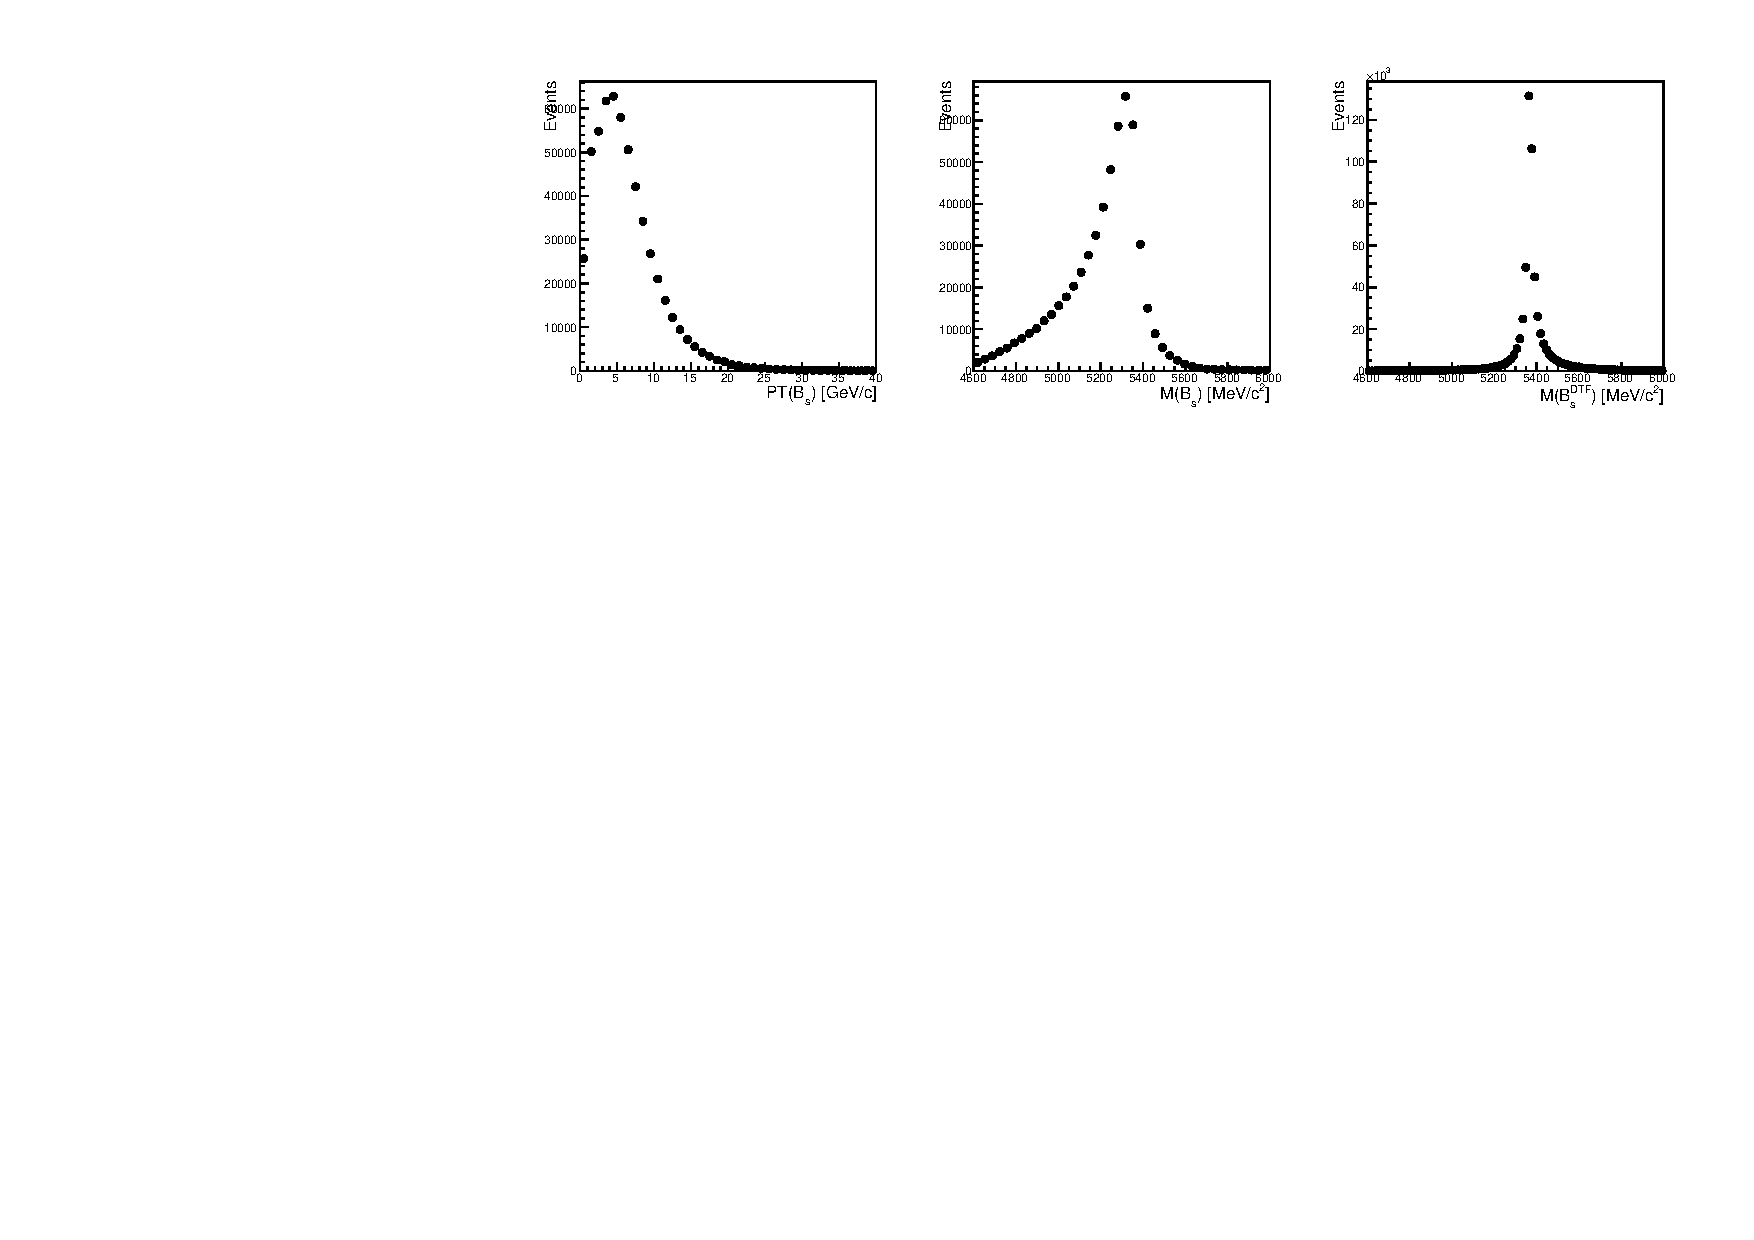
\includegraphics[width=1\linewidth]{Bkg_Bspeak/Bs_MM_MC12.pdf} \\
    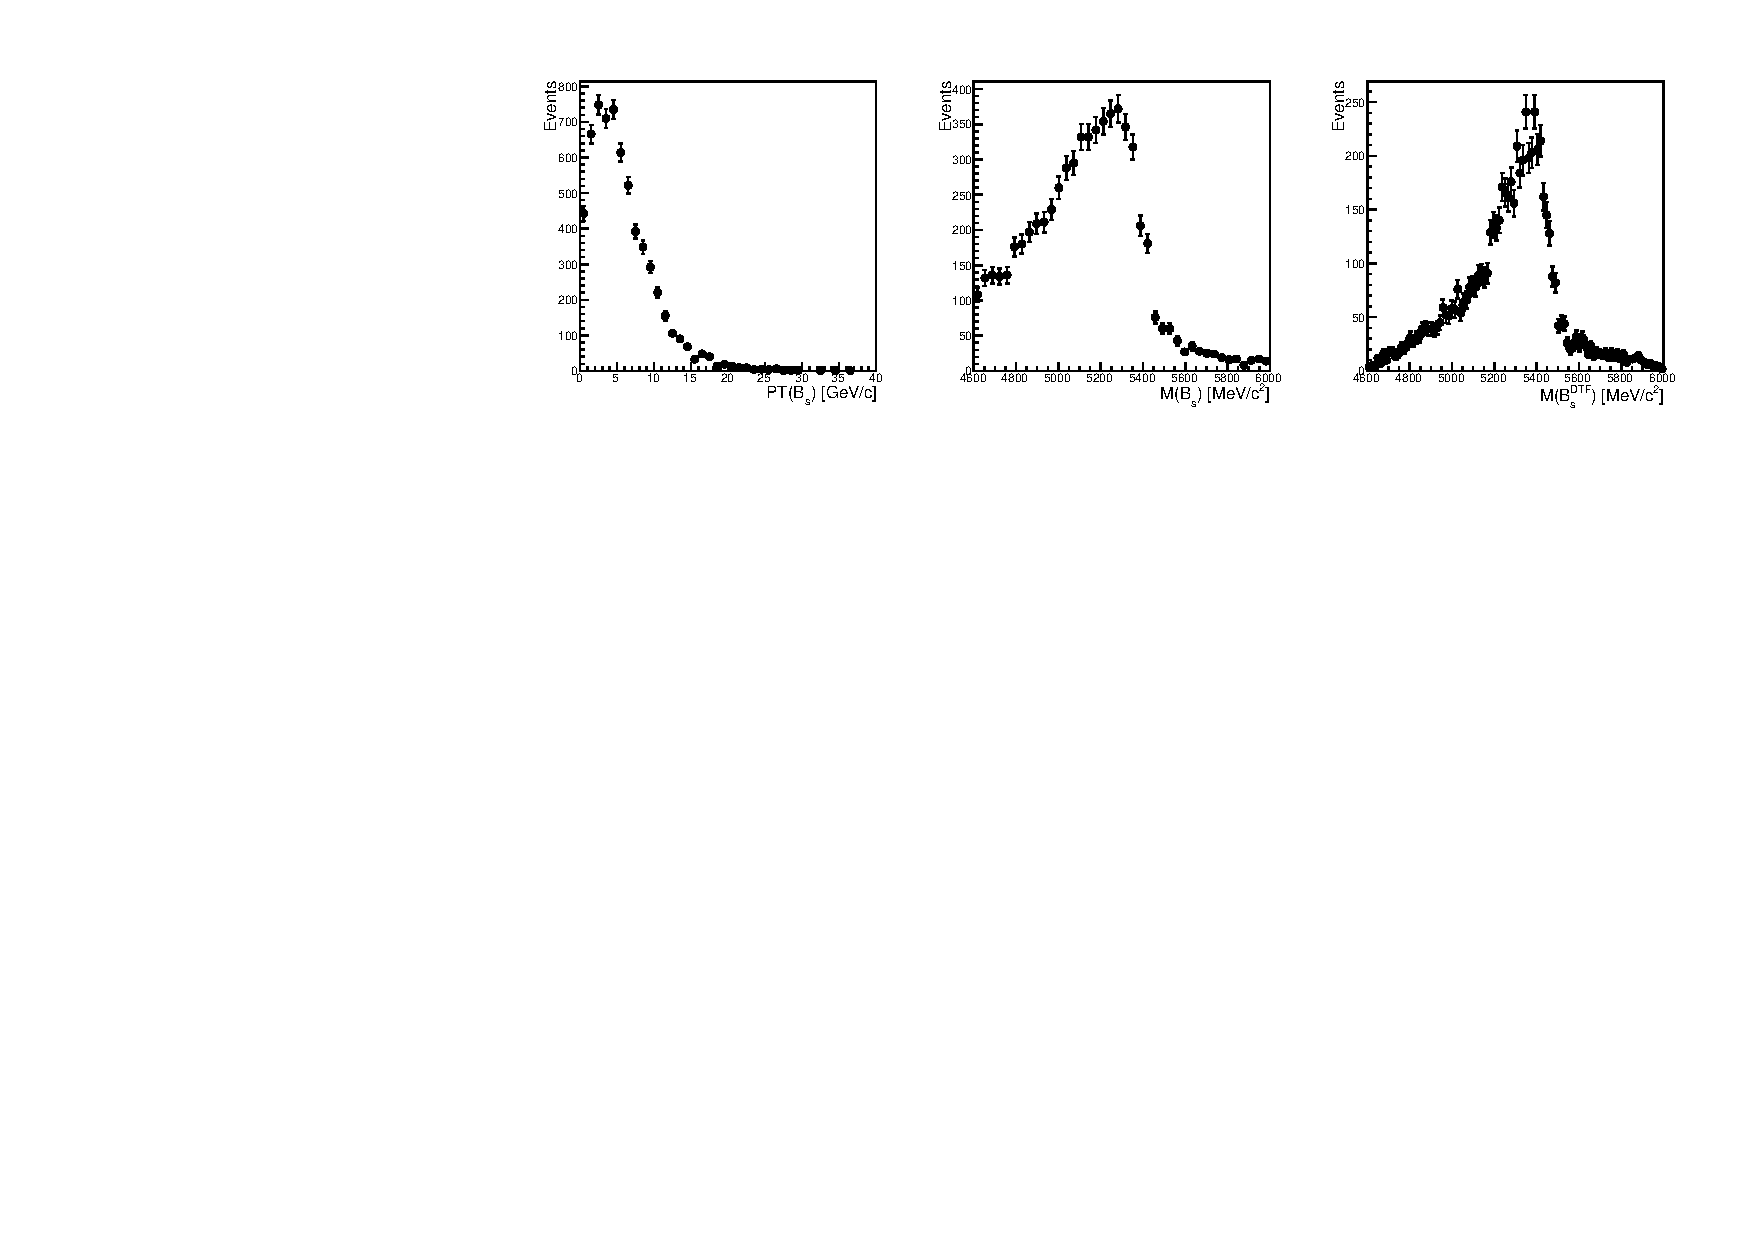
\includegraphics[width=1\linewidth]{Bkg_Bspeak/Bs_Lb2JpsipK_MM_MC12.pdf}
  \end{center}
  \caption{
   The transverse momentum and mass distributions of signal $\Bs\to\jpsi\phi$ events (top) and $\Lb\to\jpsi pK$ events reconstructed as $\Bs\to\jpsi\phi$ decay (bottom). The distributions correspond to 2012 simulated sample.   
}
  \label{fig:Bs_MM_MC12}
\end{figure}
  The transverse momentum and mass distributions of the simulated signal $\Bs\to\jpsi\phi$ and background $\Lb\to\jpsi pK$ channels are presented in Fig.~\ref{fig:Bs_MM_MC12}. The number of simulated signal events is 557 908 with 6 323 $\Lb\to\jpsi pK$ events passing through the selection.
  
To reduce the contribution of $\Lb\to\jpsi pK$ decay, a second BDT is trained using the following samples:
 \begin{itemize}
   \item Signal: the simulated $\Bs\to\jpsi\phi$ sample is used as the signal model. This sample is required to pass exactly the same stripping and preselection criteria as described in Sec.~\ref{subsec:EvtSel}. Furthermore the MC truth information is used to require that the reconstructed candidate matches with the generated decay.
   \item Background: the simulated $\Lb\to\jpsi pK$ sample reconstructed as a signal channel is used. Also these events are required to pass all the selection steps.
  \end{itemize}
 A set of 13 kinematic variables is taken as an input for the BDT discriminator, where 12 variables are the same as used in the first BDT training (Sec.~\ref{subsec:BDT}). The additional variable is the log-likelihood of the proton hypothesis for a kaon and it is the variable with the largest importance for the BDT technique. The ranking of the variable importance used to train the BDT is shown in Table~\ref{tab:RankingBDT2}. The plots comparing the input variable distributions between signal and background are shown in Appendix~\ref{sec:app:BDT}.
 
 \begin{table}[htb]
  \caption{
    The ranking of the variable importance used in peaking background BDT selection.
}
    \small{
\begin{center} \begin{tabular}{ccc}
    \hline
   Rank&Variable & Importance  \\
    \hline
  1&log(ProbNNp)($K^{+}$) & 1.503e-01 \\
  2&log(ProbNNK)$(K^{-})$ & 1.413e-01 \\
  3&$\chi^{2}_{\text{vtx}}(B^{0}_{s})$ & 1.338e-01 \\
  4&log$(\chi^{2}_{\text{IP}})(e^{+})$ & 1.316e-01 \\
  5&log$(\chi^{2}_{\text{IP}})(e^{-})$ & 9.461e-02 \\
  6&log(ProbNNK)$(K^{+})$ & 8.547e-02 \\
  7&$p_{T}(J/\psi)$ & 8.475e-02 \\
  8&$p_{T}(\phi)$ & 7.417e-02 \\
  9&PIDe$(e^{-})_{\text{corr}}$ & 3.015e-02 \\
  10&IP$(B^{0}_{s})$ & 2.547e-02 \\
  11&PIDe$(e^{+})_{\text{corr}}$ & 2.455e-02 \\
  12&log$(\chi^{2}_{\text{DTF}})(B^{0}_{s})$ & 2.387e-02 \\
  13&$\chi^{2}_{\text{FD}}(B^{0}_{s})$ & 0.000e+00 \\
  \hline
    \end{tabular}\end{center}
  }
\label{tab:RankingBDT2}
\end{table}

In the case of second BDT training, the BDT classifier distribution doesn't have a good separation of signal from background since the variables for trained samples have similar distributions and values (Fig.~\ref{fig:BDTLbresponse}a). For these reasons, it is not possible to build a FoM based on sWeights. Therefore a new figure of merit (FoM2) is used to define a selection criterium:
\begin{equation}\label{eq:FoM2}
   FoM2=\frac{S}{\sqrt{S+B1+B2}},
  \end{equation}
where $S$, $B1$ and $B2$ are the number of the signal and two types of the background events, respectively. The $B1$ and $B2$ background events are defined by the exponential and Gaussian functions, respectively. A two Crystal Ball functions with a common mean determine the signal shape. The mass fits are shown in Sec.~\ref{sec:BsFit}. The dependence of the FoM2 value on BDT response cut is shown in Fig.~\ref{fig:BDTLbresponse}b. All FoM values are consistent to each other within the limits of uncertainty. The optimal cut of $>$0.15 is chosen to select the final data sample. 
\begin{figure}[ht!]
  \begin{center}
    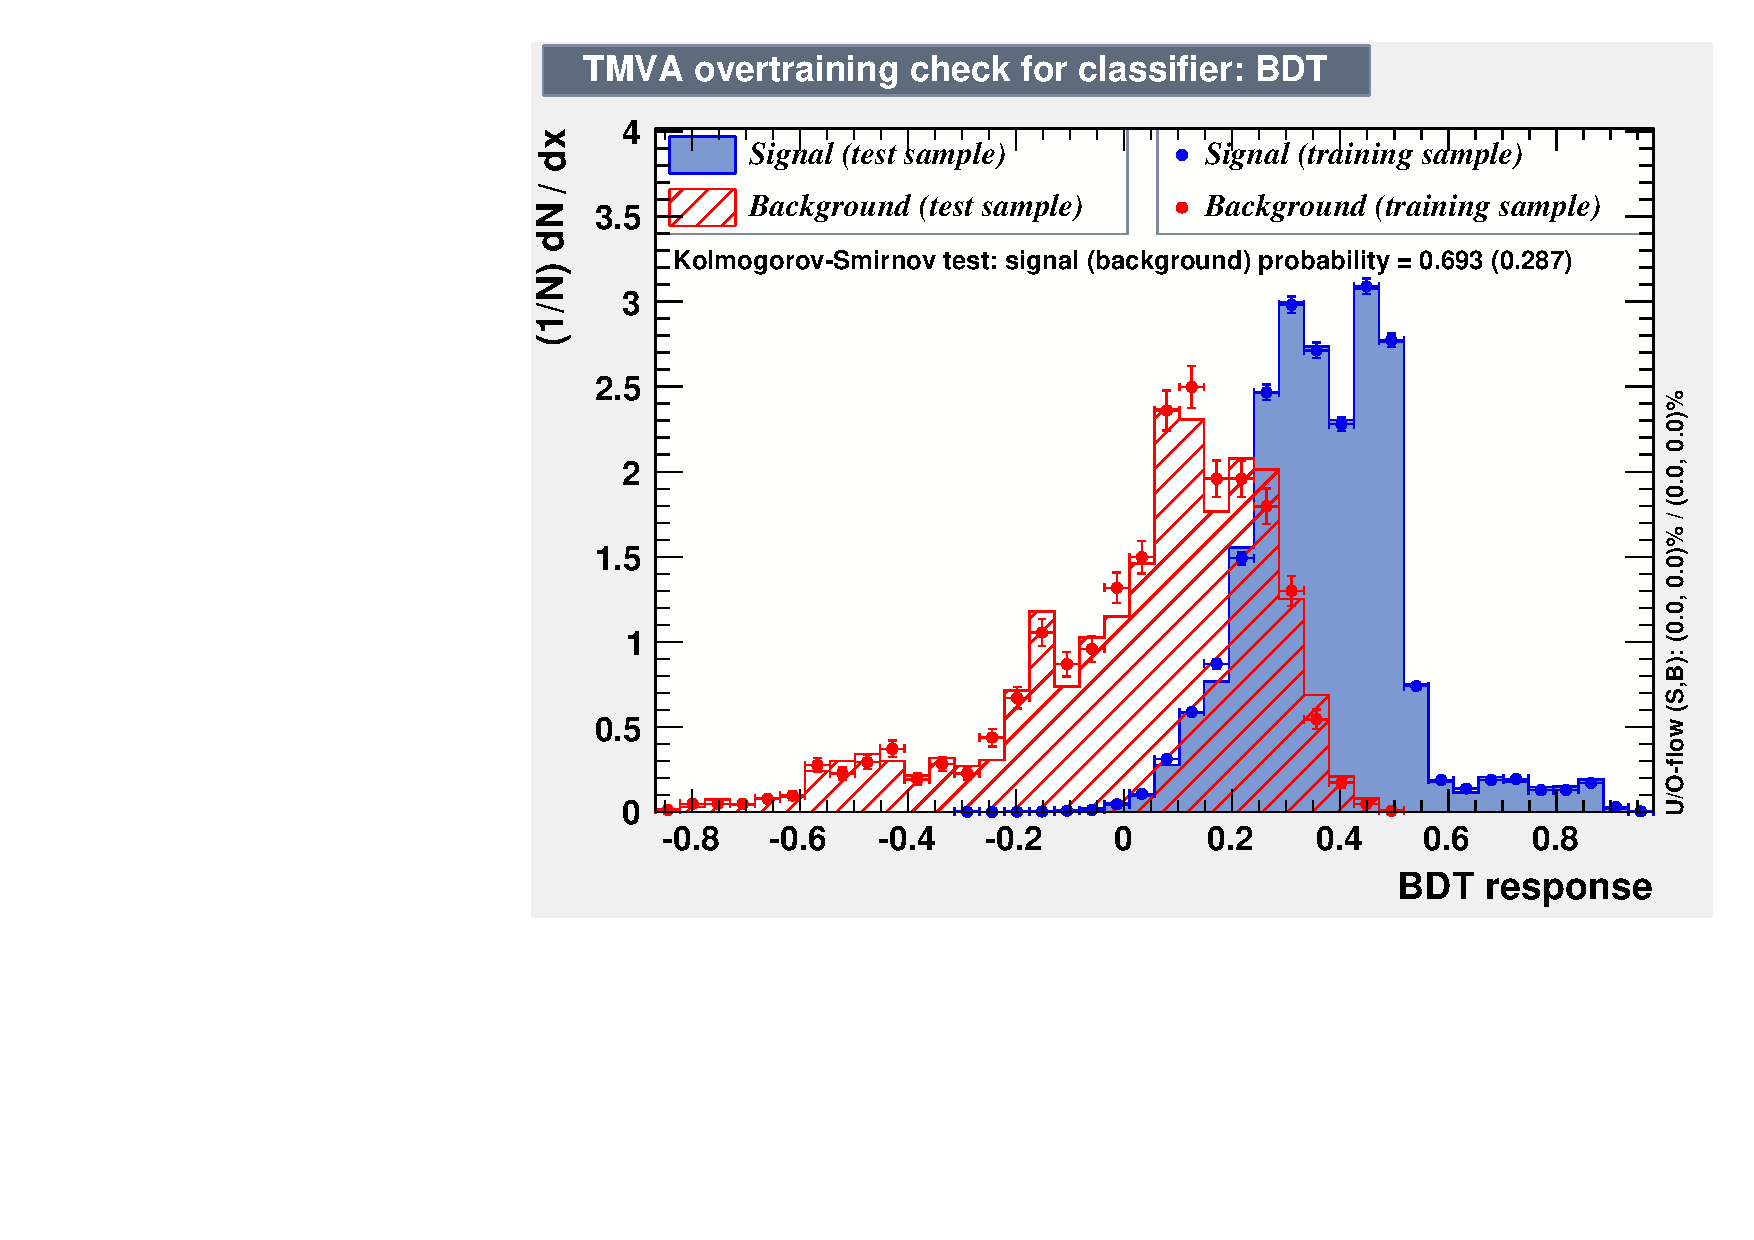
\includegraphics[width=0.49\linewidth]{BDT/BDTLb_response_bkgcat0_wSPDHits_trigger_RD12.pdf}\put(-115,-13){(a)}
    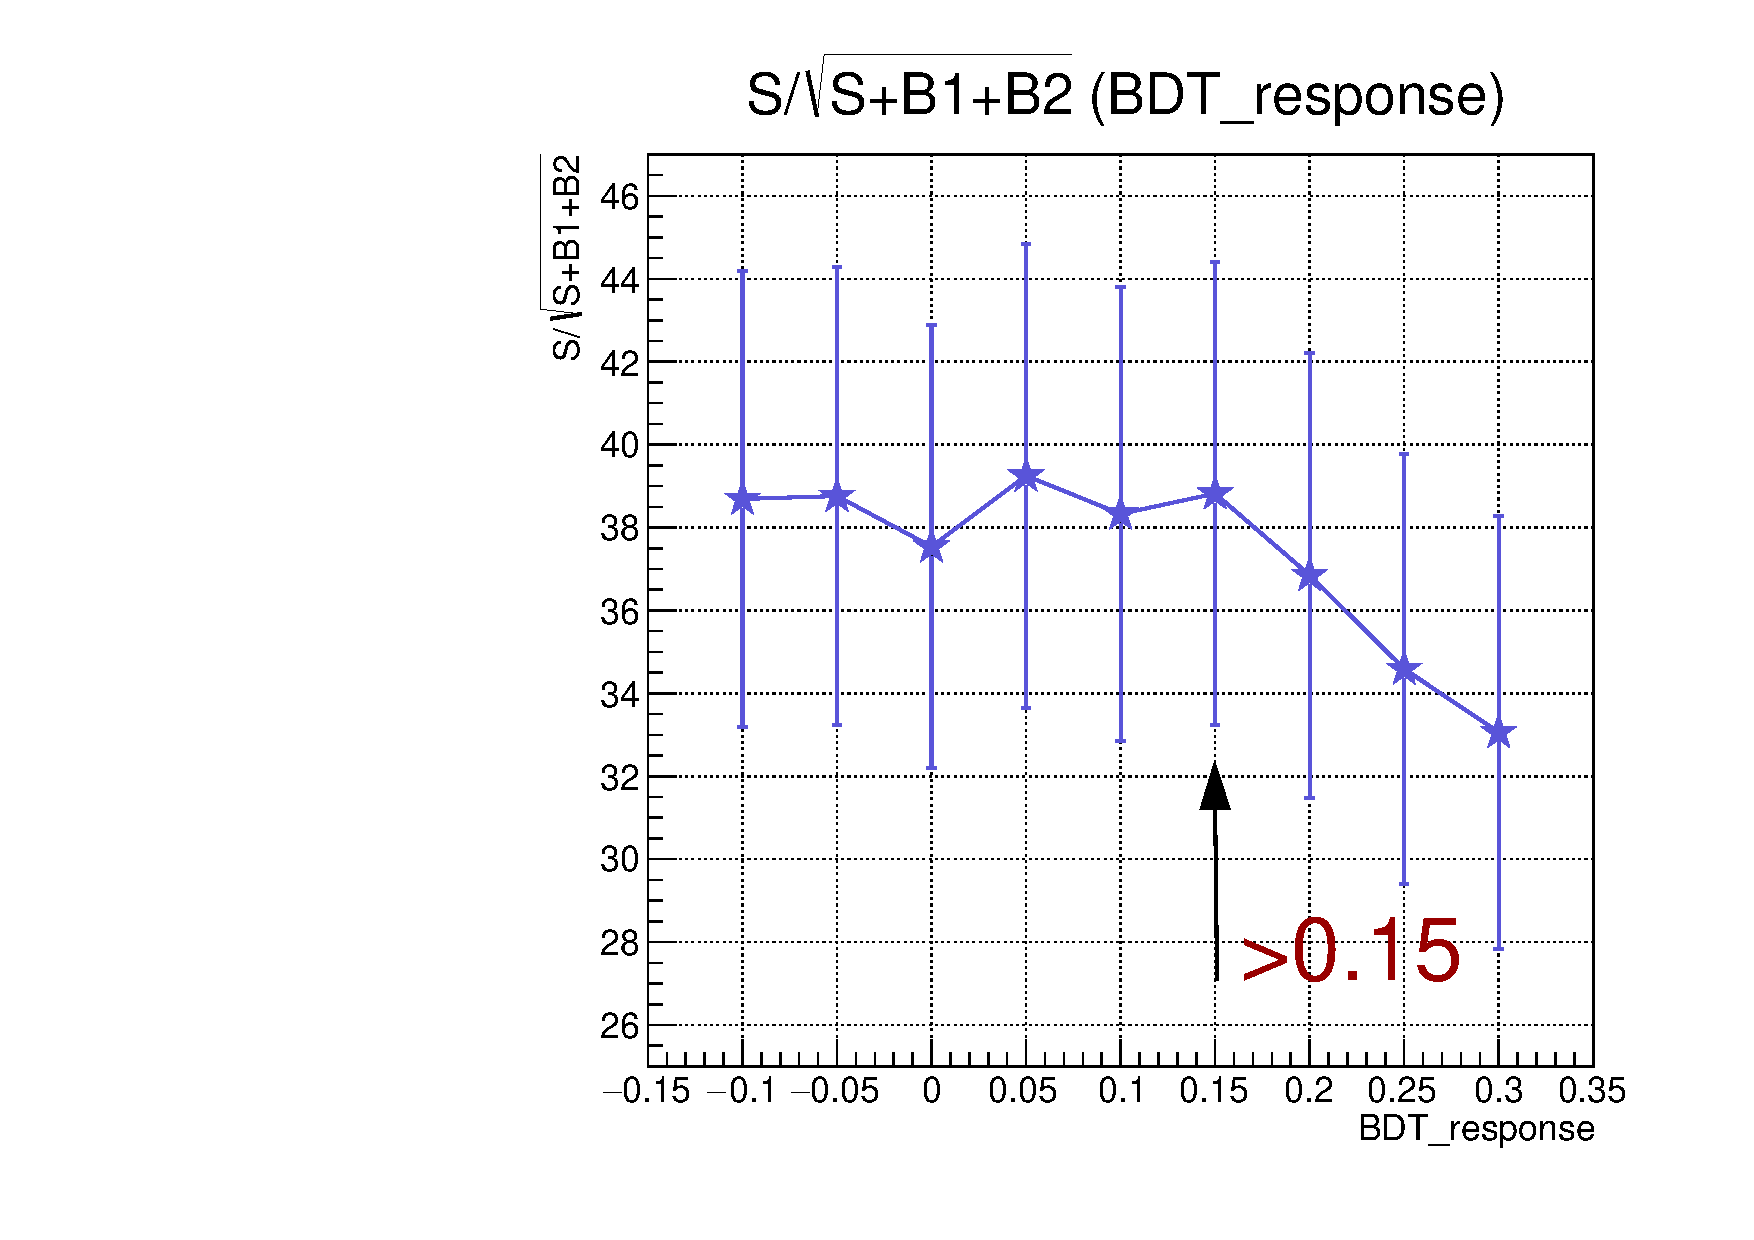
\includegraphics[width=0.4\linewidth]{BDT/FoM_BDTLb_response.pdf}\put(-115,-13){(b)}
  \end{center}
  \caption{
   (a) The distributions of the peaking background BDT classifier for $\Bs\to\jpsi\phi$ training samples. The signal is red hatched filled while background is blue solid filled. (b) The distribution of the FoM2 value in depends on the BDT response cut.  
}
  \label{fig:BDTLbresponse}
\end{figure}

After applying this cut the number of the $\Lb\to\jpsi pK$ events is in the MC sample has decreased by 44.5$\%$. This corresponds to decrease the number of $\Bs\to\jpsi\phi$ candidates by 4.2$\%$ for the data sample.   
\clearpage
  
\section{Mass fit}\label{sec:BsFit}

The $\jpsi$ and $\phi$ mass fit result after all selection steps (Sec.~\ref{subsec:EvtSel}-\ref{subsec:PeakBkg}) using 3~$\invfb$ data sample is presented in Fig.~\ref{fig:JpsiPhimass}. The $\jpsi$ mass fit is performed using a sum of two Crystal Ball functions with a common mean for the signal and a polynomial function for the background events. In case of the $\phi$ meson, as a mass model a sum of double Gaussian and Voigtian functions~\cite{OLIVERO1977233} is used with a common mean for the signal candidates and a Chebychev polynomial for the background. The signal and the background yields from the fits to the two mesons are performed separately for 2011 and 2012 and the results are shown in Table~\ref{tab:JpsiPhiTable}.
\begin{figure}[htb]
  \begin{center}
    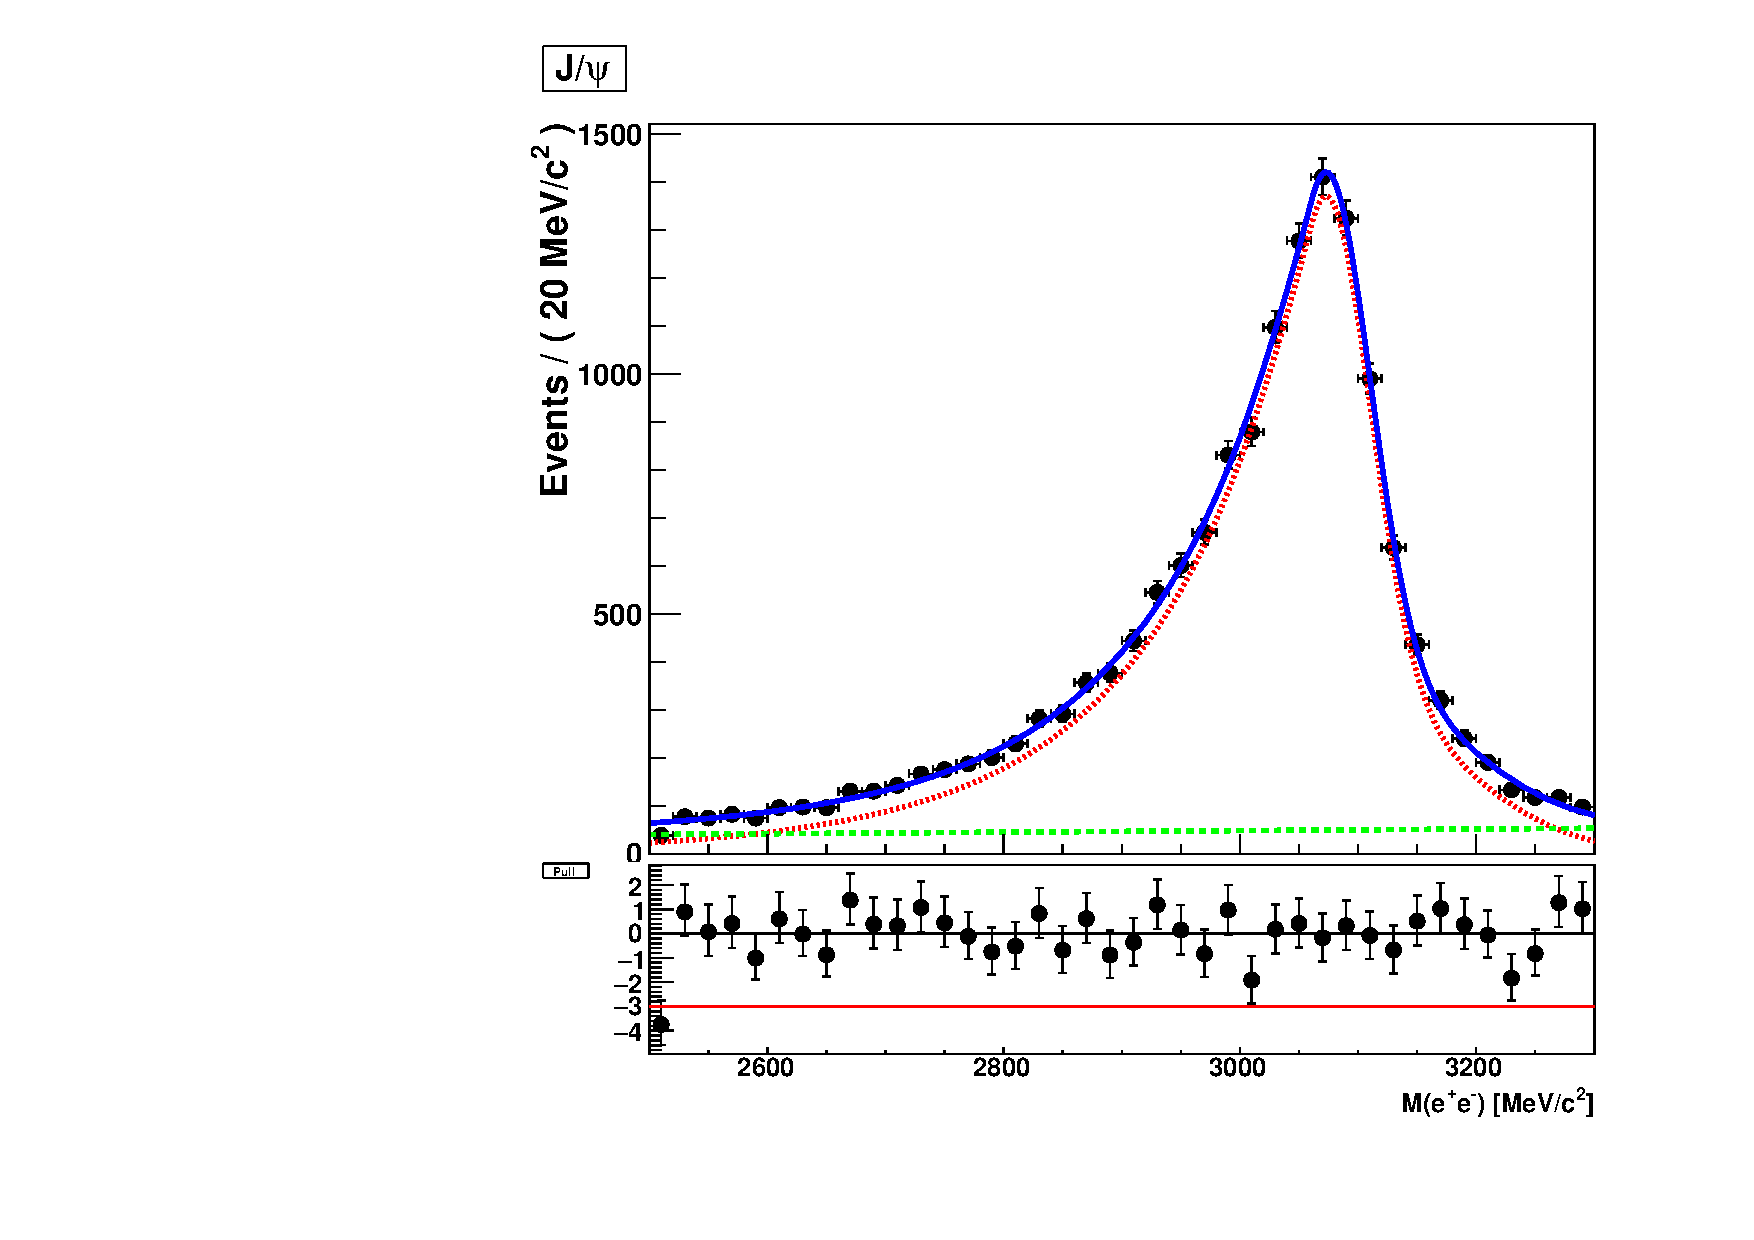
\includegraphics[width=0.49\linewidth]{RDfull_BDT1_BDT2_sWeight/mdau1.pdf}\put(-115,-4){(a)}
    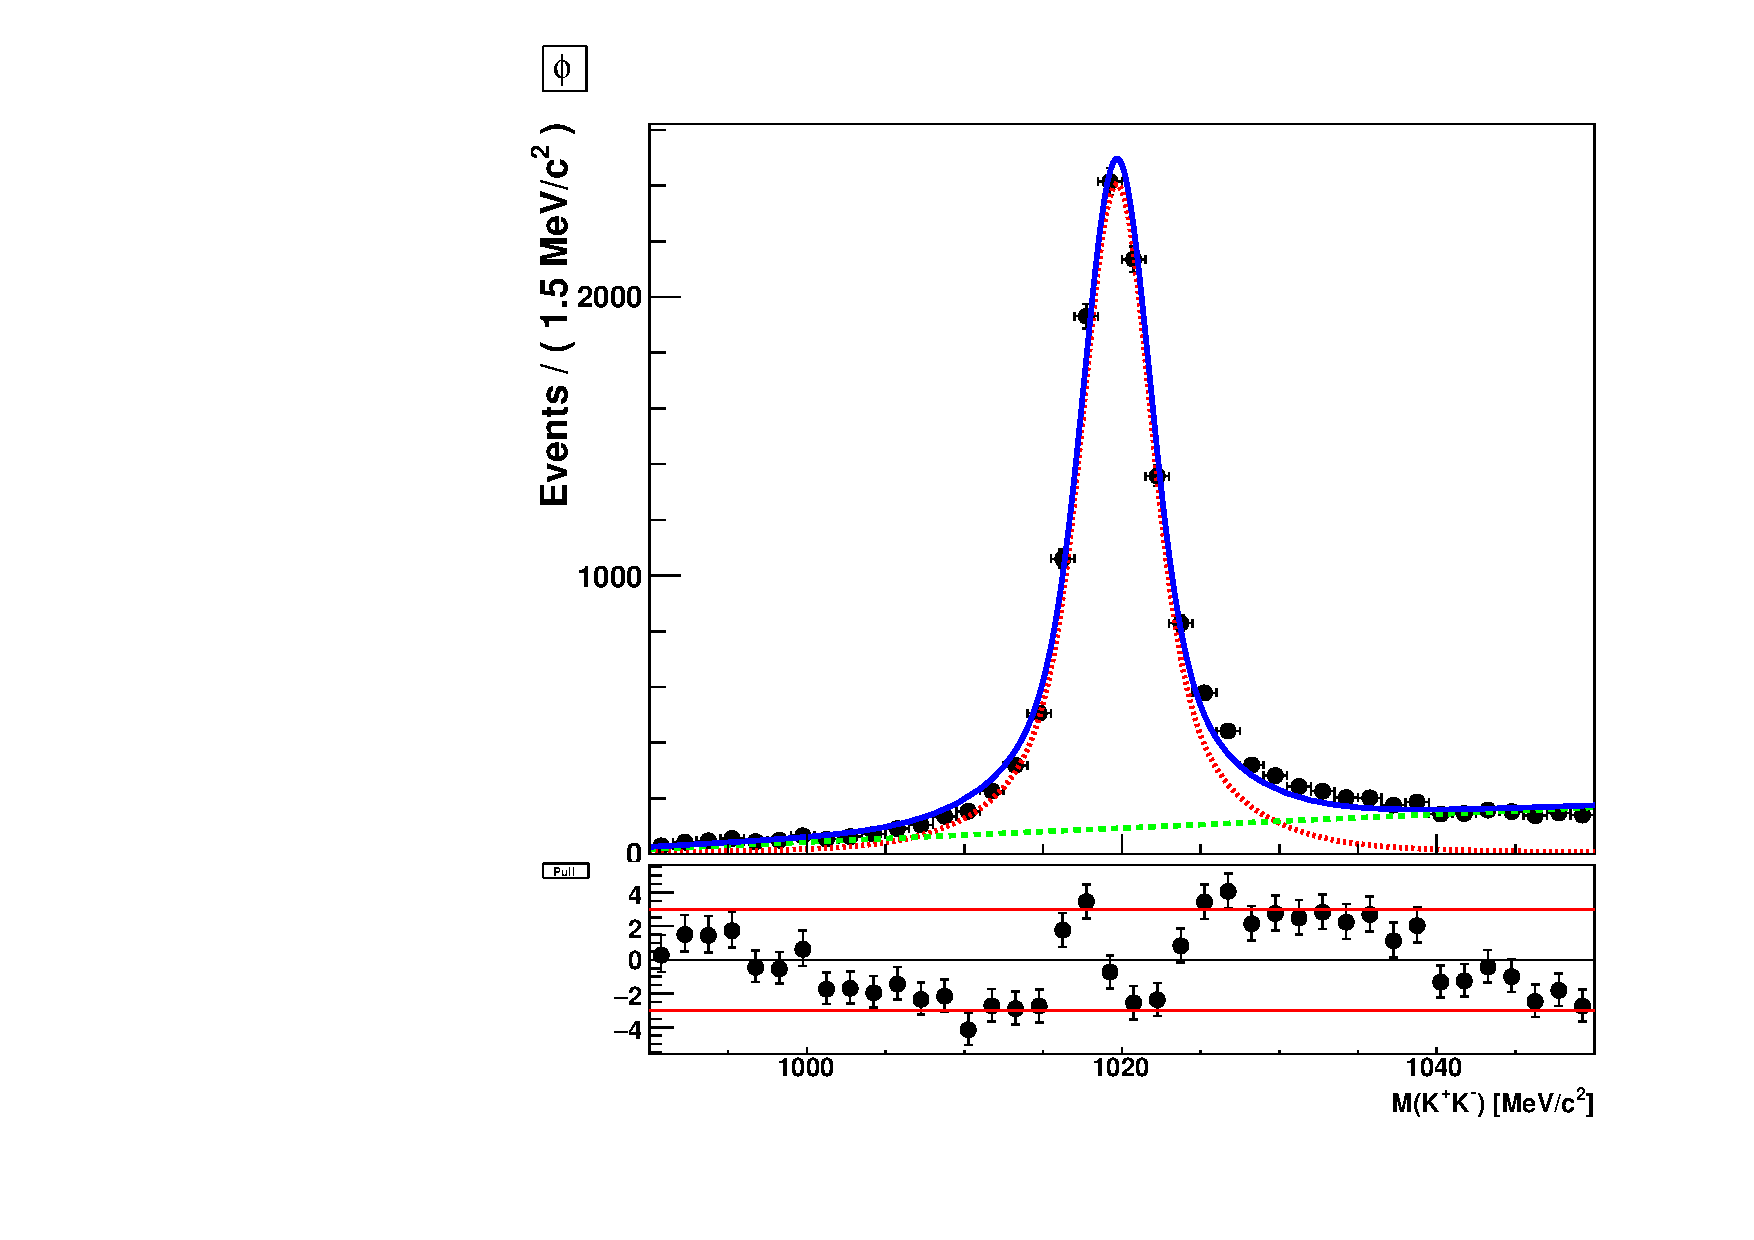
\includegraphics[width=0.49\linewidth]{RDfull_BDT1_BDT2_sWeight/mdau2.pdf}\put(-115,-4){(b)}
  \end{center}
  \caption{
   The invariant mass distributions of the (a) $\jpsi\to\epem$ and (b) $\phi\to\Kp\Km$ systems for the selected data sample of $\Bs\to\jpsi\phi$ candidates. The solid blue line shows the total fit, the signal and combinatorial background components are given by dotted red line and dashed green line, respectively.
}
  \label{fig:JpsiPhimass}
\end{figure}
\begin{table}[htb]
  \caption{
    The signal and the background yields from fits to the $\jpsi$ and $\phi$ mass distributions, separately in 2011 and 2012.
}
\small{
\begin{center} \begin{tabular}{|c|c|c|}
    \hline
   Year & 2011 & 2012  \\
    \hline
  $\jpsi$ bkg & 771$\pm$57 & 1 525$\pm$88\\
  $\jpsi$ signal & 3 833$\pm$79 & 9 551$\pm$126\\
  \hline
  \hline
  $\phi$ bkg & 990$\pm$48 & 2 632$\pm$69\\
  $\phi$ signal & 3 613$\pm$70 & 8 444$\pm$103\\
  \hline
    \end{tabular}\end{center}
  }
\label{tab:JpsiPhiTable}
\end{table}

For the $\Bs$ mass fit a signal model composed of a two Crystal Ball functions with a common mean is performed. The background model consists of an exponential fucntion for the combinatorial component and a Gaussian function for the partially reconstructed events (Fig.~\ref{fig:Bsmass}a). The partially reconstructed background (Bkg2) consists mainly of excited charmonium resonances and will be described in Sec.~\ref{subsubsec:PartRecBkg}. The fitted parameter values for the two 2011 and 2012 data samples are given in Table~\ref{tab:BsTable}, along with the signal and two background yields. 

\begin{figure}[htb!]
  \begin{center}
  \begin{minipage}[t]{0.48\linewidth}
  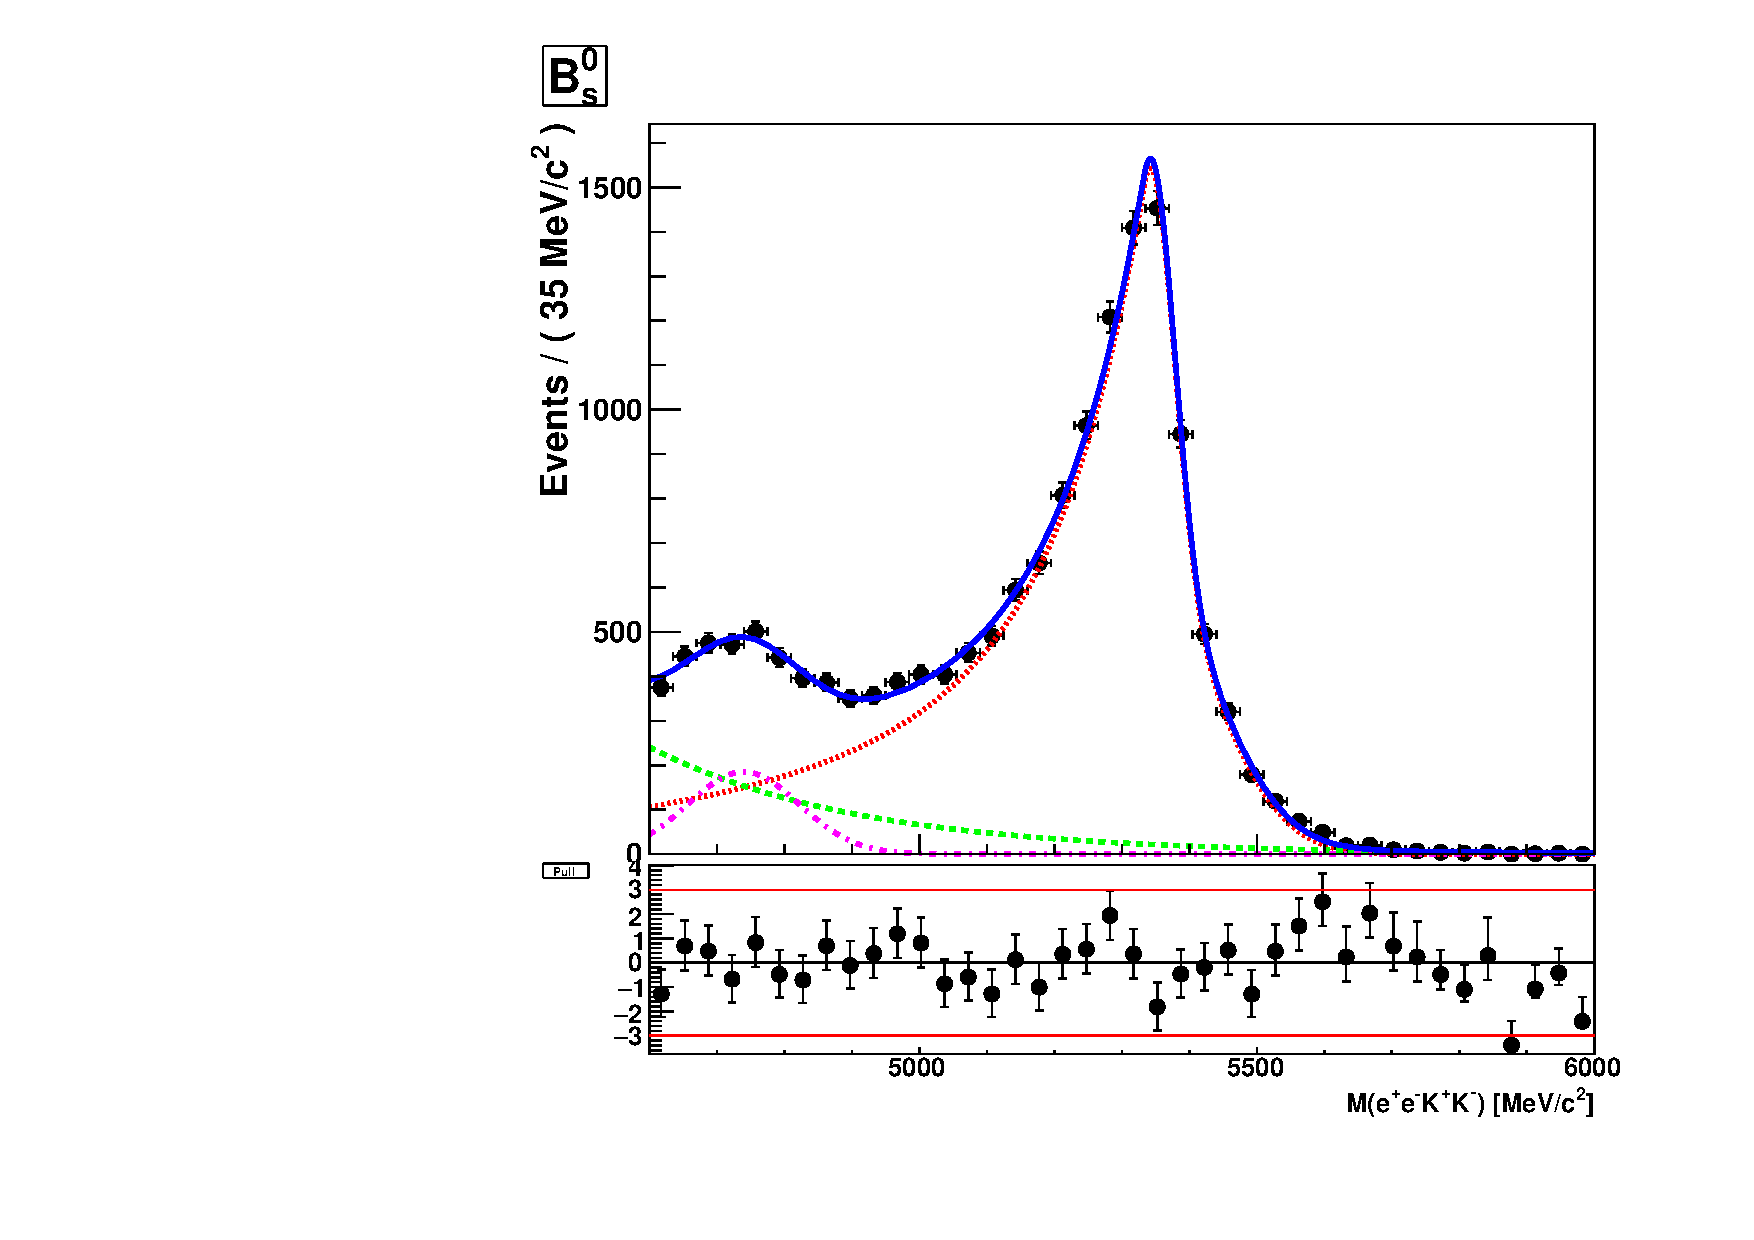
\includegraphics[width=1.1\linewidth]{RDfull_BDT1_BDT2_sWeight/mass_std.pdf}
  \end{minipage}
  \hfill
  \begin{minipage}[t]{0.48\linewidth}
  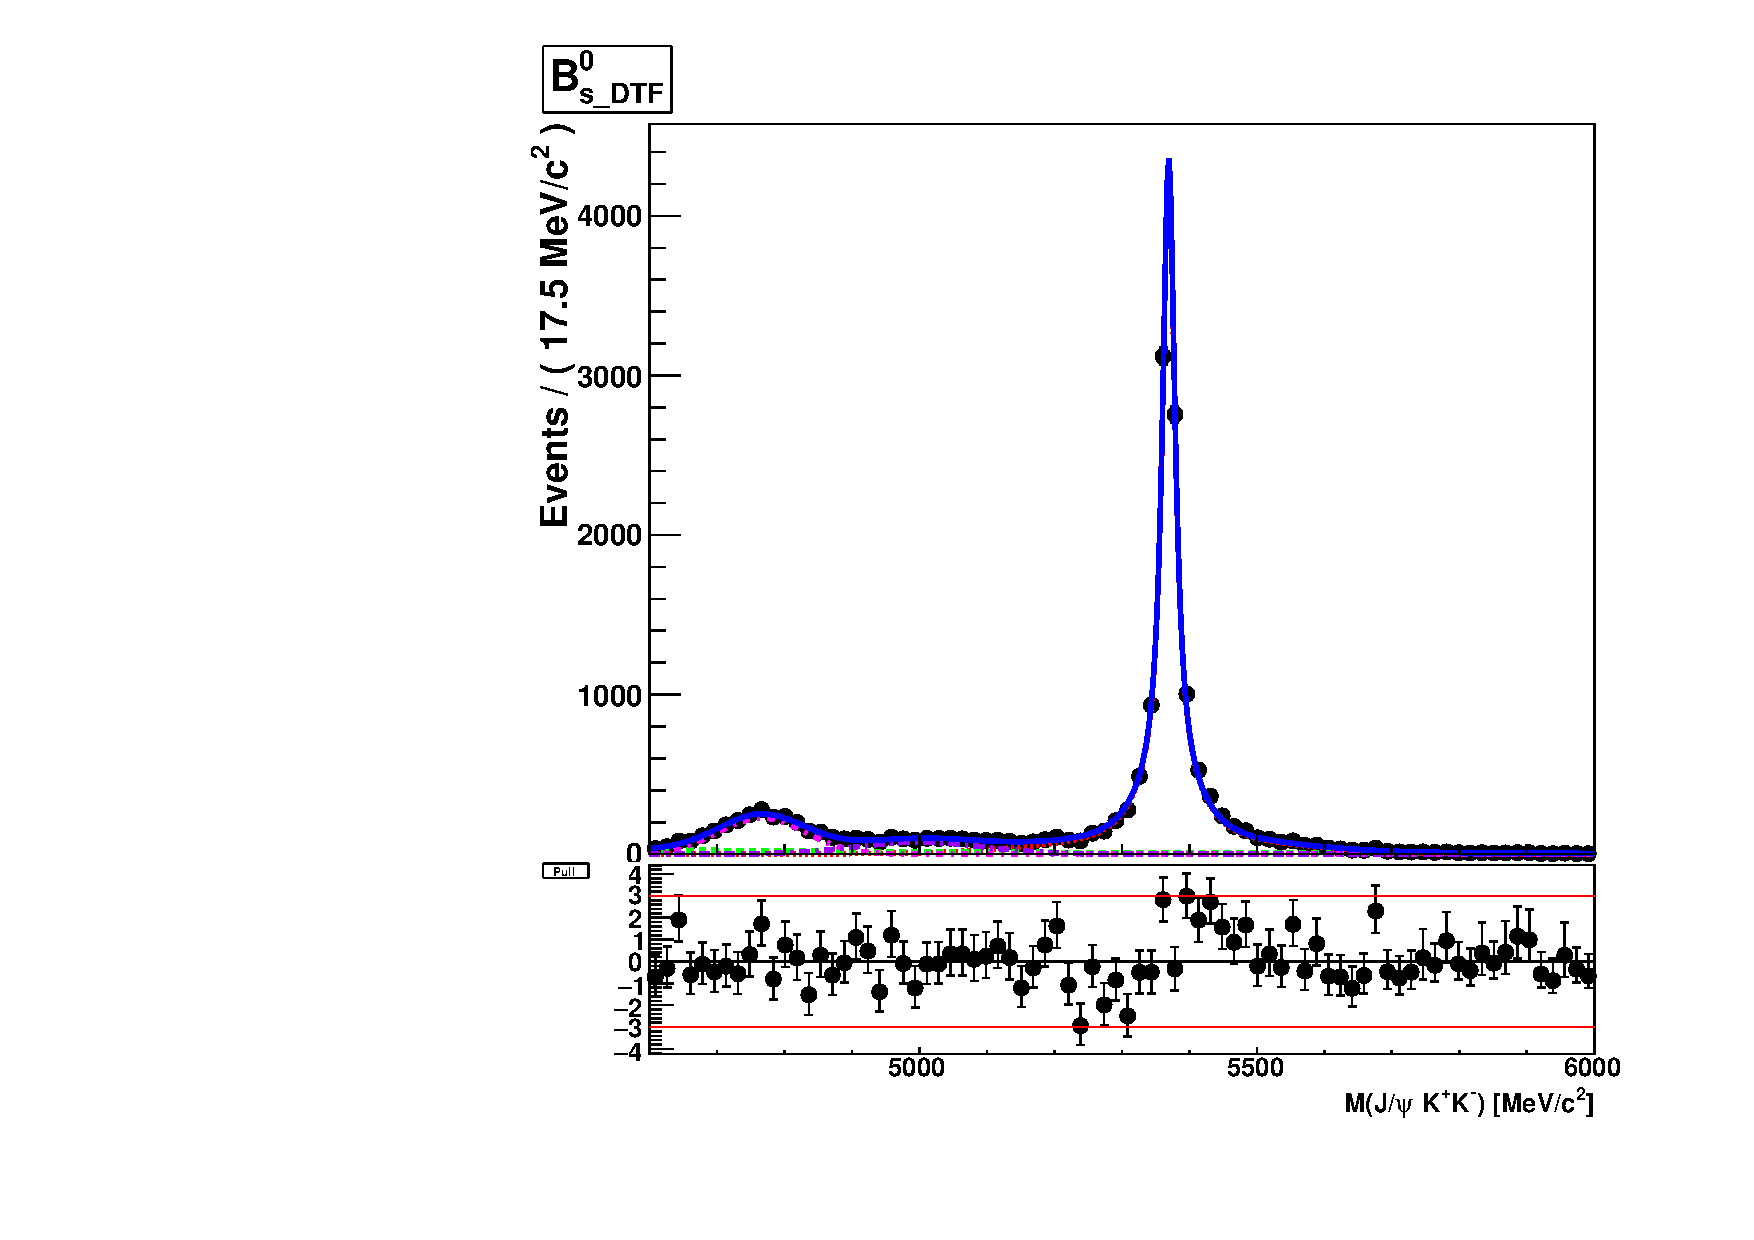
\includegraphics[width=1.1\linewidth]{RDfull_BDT1_BDT2_sWeight/mass.pdf}
  \end{minipage}
  \begin{minipage}[t]{0.48\linewidth}
  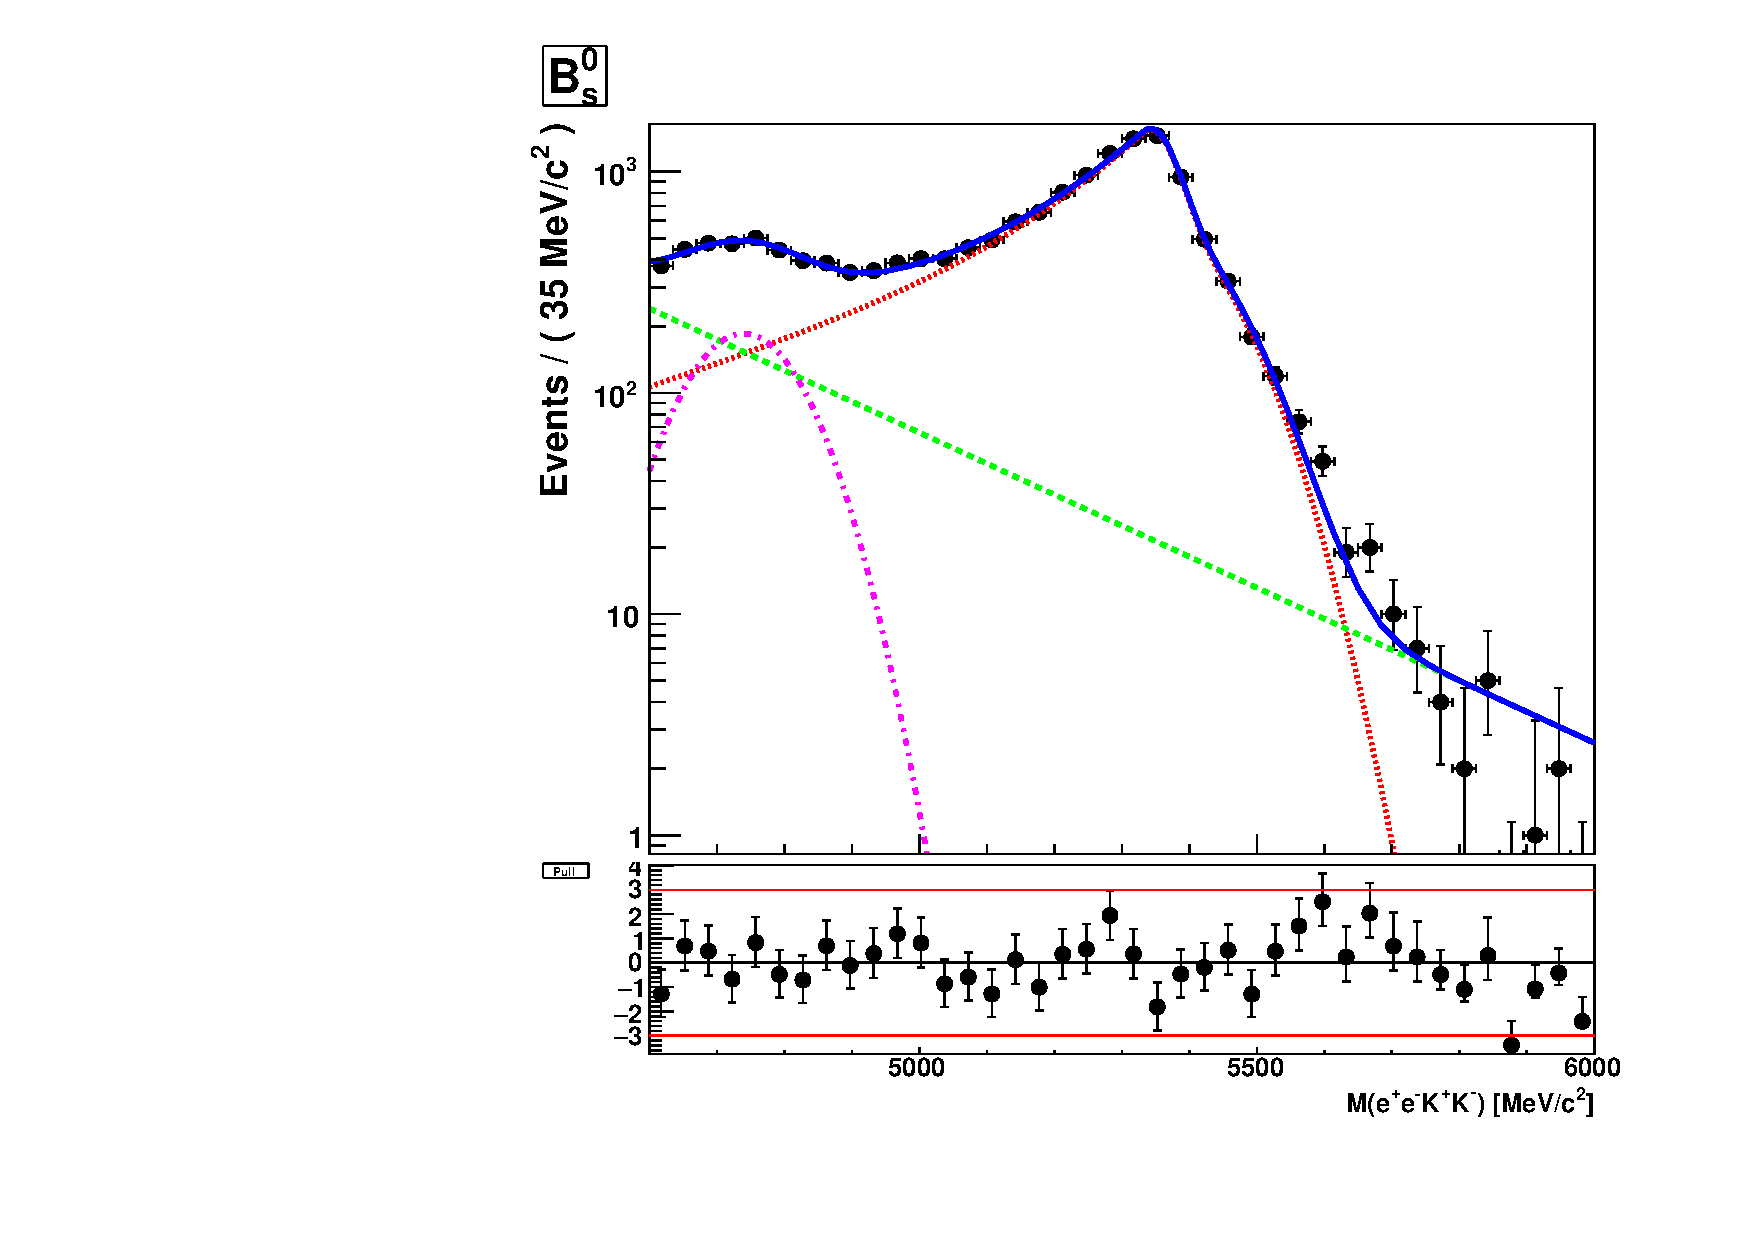
\includegraphics[width=1.1\linewidth]{RDfull_BDT1_BDT2_sWeight/mass_std_log.pdf}\put(-115,-4){(a)}
  \end{minipage}
  \hfill
  \begin{minipage}[t]{0.48\linewidth}
  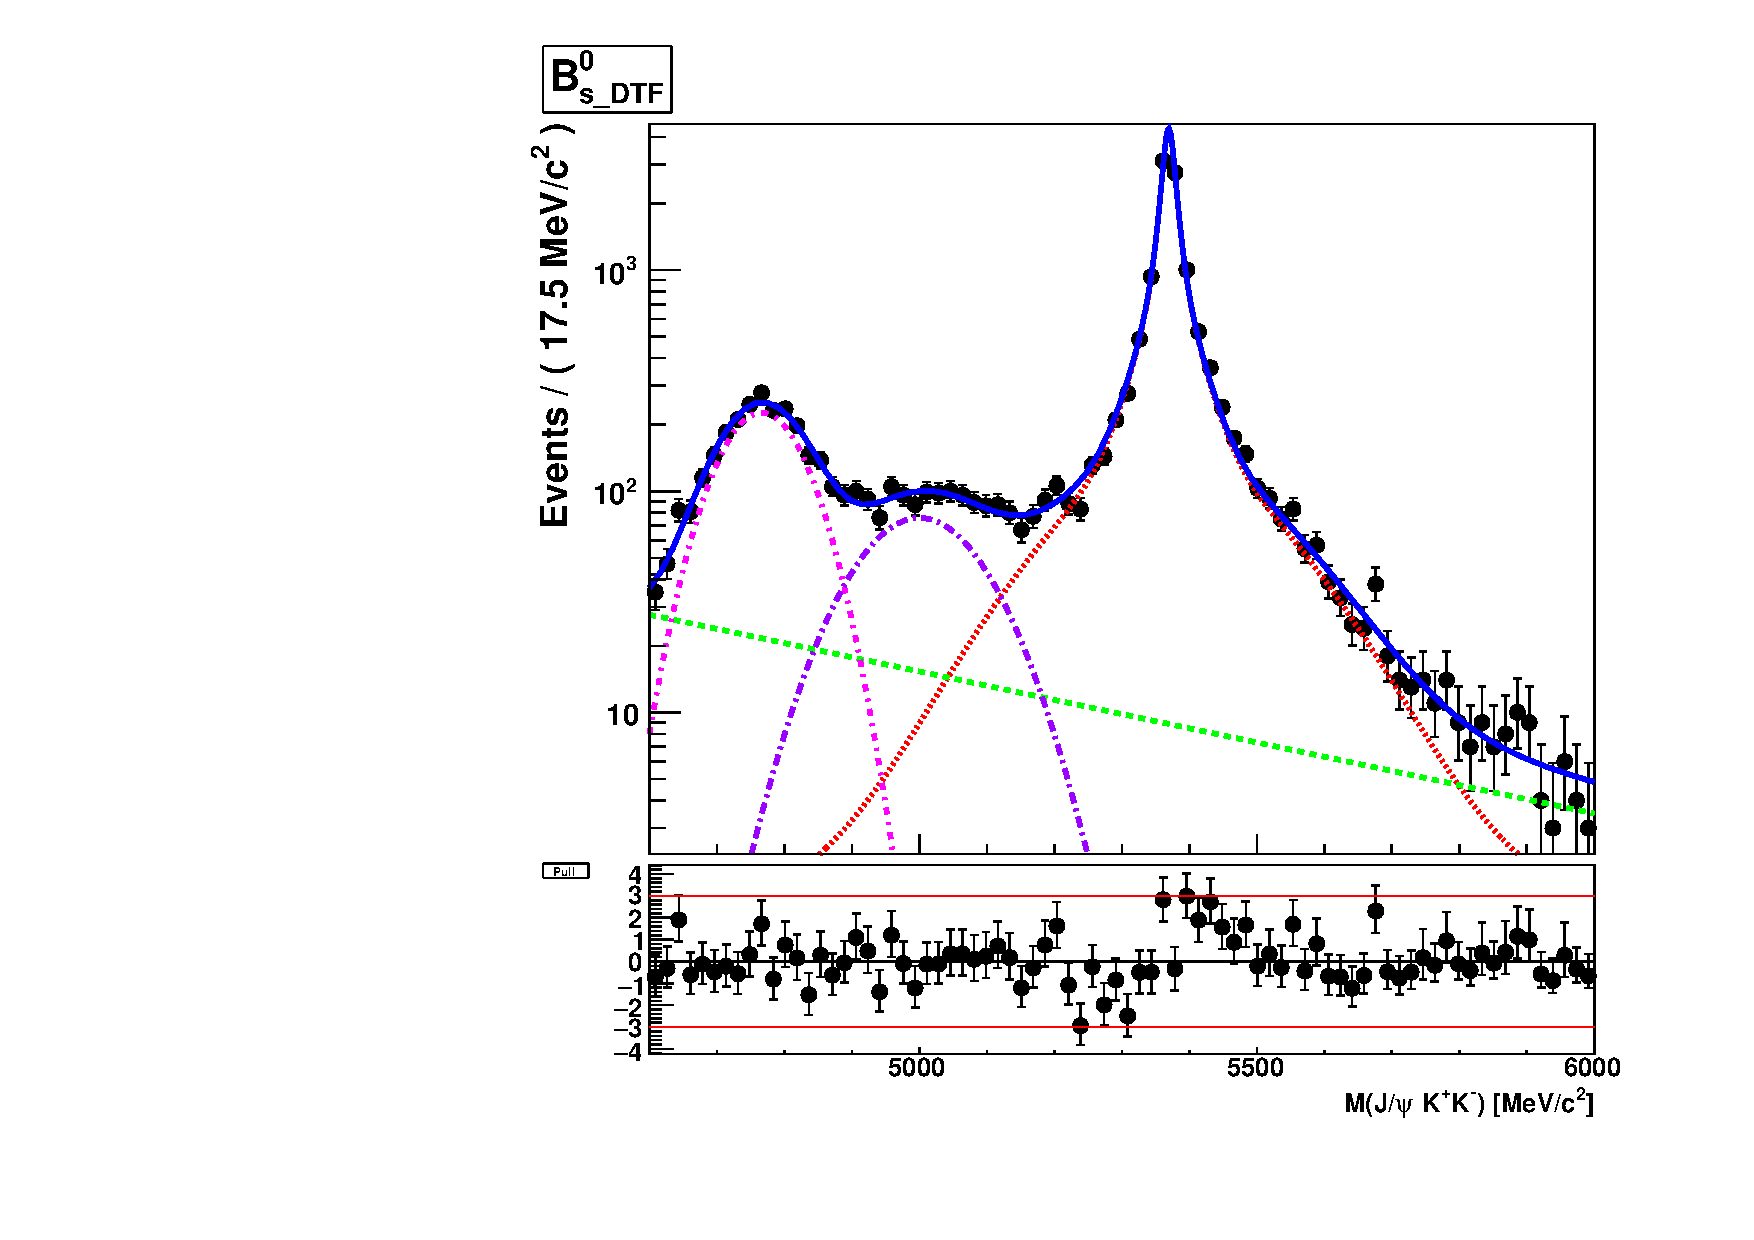
\includegraphics[width=1.1\linewidth]{RDfull_BDT1_BDT2_sWeight/mass_log.pdf}\put(-115,-4){(b)}
  \end{minipage}
  \end{center}
  \caption{
   The invariant mass distributions of the (a) $\Bs$ and (b) $\Bs$ using DTF in the selected data sample of $\Bs\to\jpsi\phi$ candidates. The solid blue line shows the total fit, the signal and combinatorial background components are given by dashed red line and dotted green line, respectively. The partially reconstructed background contributions are given by dash-dotted pink and violet lines. The top and bottom plots are linear and logarithmic scale, respectively.
}
  \label{fig:Bsmass}
\end{figure}

The $\Bs$ mass distribution with the mass of $\epem$ system constrained to the PDG mass of $\jpsi$~\cite{PDG2014}, obtained using Decay Tree Fitter (DTF), is shown in Fig.~\ref{fig:Bsmass}b. The mass model is a sum of double Gaussian and Breit-Wigner functions with a common mean for the signal candidates. The model describing combinatorial background is an exponential, two Gaussian functions are used to describe the partially reconstructed background (Sec.~\ref{subsubsec:PartRecBkg}). The fitted parameter values for the two 2011 and 2012 data samples are shown in Table~\ref{tab:BsDTFTable}, along with the signal and three  background yields. The number of signal events is 11 645$\pm$114 for the full 2011 and 2012 data sample, which corresponds to 12$\%$ of the signal events from the $\mumu$ decay mode of $\Bs\to\jpsi\phi$. 

The mass fit results for the $\Bs$ without and with DTF are in agreement to each other. The $\Bs$ mass distributions in a logarithmic scale are shown in Fig.~\ref{fig:Bsmass}.

\begin{table}[hb]
  \caption{
    The results of the fit to the $\Bs$ mass distribution, separately for 2011 and 2012 data samples. The signal shape is modeled by a sum of the two Crystal Ball functions with a common mean. The partially reconstructed background is modeled as a Gaussian function. The combinatorial background shape is an exponential.
}
\small{
\begin{center} \begin{tabular}{|c|c|c|}
   \hline
      Parameter & 2011 & 2012  \\
    \hline
   $\alpha^{CB}_{1}$ & 1.90$\pm$0.510 & 2.60$\pm$1.20\\
   $\alpha^{CB}_{2}$ & 0.10$\pm$0.062 & 0.15$\pm$0.02\\
   $\sigma_{1}$[$\mevcc$] & 100$\pm$3.1 & 100$\pm$0.45  \\
   $\sigma_{2}$[$\mevcc$] & 29$\pm$3.3 & 33$\pm$1.4  \\
   $\sigma_{Bkg2}$[$\mevcc$] & 68$\pm$26 & 74$\pm$8.3  \\
   $\mu$[$\mevcc$] & 5 353$\pm$3.9 & 5 349$\pm$1.7 \\
   $\mu_{Bkg2}$[$\mevcc$] & 4 739$\pm$20 & 4 734$\pm$8.8  \\
   $f$ & 0.336$\pm$0.070 & 0.304$\pm$0.053  \\
   Bkg slope & -0.0034$\pm$0.0004 & -0.0031$\pm$0.00002 \\
   N$_{Bkg1}$ & 689$\pm$77 & 586$\pm$76  \\
   N$_{Bkg2}$ & 258$\pm$48 & 1 163$\pm$123 \\
   N$_{Sig}$ & 3 656$\pm$73 & 9 327$\pm$119 \\
  \hline
    \end{tabular}\end{center}
  }
\label{tab:BsTable}
\end{table}
\begin{table}[htb]
  \caption{
    The results of the fit to the $\Bs$ mass distribution with DTF, separately for 2011 and 2012 data samples. The signal shape is a sum of double Gaussian and Breit-Wigner functions with a common mean. The two partially reconstructed backgrounds are modeled by two Gaussians. The combinatorial background shape is an exponential function.
}
\small{
\begin{center} \begin{tabular}{|c|c|c|}
    \hline
   Parameter & 2011 & 2012  \\
    \hline
  $\sigma_{1}$[MeV/c$^{2}$] & 147$\pm$23 &158$\pm$12\\
  $\sigma_{2}$[MeV/c$^{2}$] & 8.1$\pm$0.92 &45$\pm$6.3\\
  $\sigma_{3}$[MeV/c$^{2}$] & 50$\pm$11 &23$\pm$1.1\\
  $\sigma_{bkg2}$[MeV/c$^{2}$] & 60$\pm$6.3 &65$\pm$4.4\\
  $\sigma_{bkg3}$[MeV/c$^{2}$] & 109$\pm$20 &90$\pm$9.2\\
  $f_{1}$ & 0.11$\pm$0.035 &0.17$\pm$0.017\\
  $f_{2}$ & 0.24$\pm$0.065 &0.12$\pm$0.026\\
  $\mu$[MeV/c$^{2}$] & 5370$\pm$0.36 &5370$\pm$0.23\\
  $\mu_{bkg2}$[MeV/c$^{2}$] & 4757$\pm$5.2 & 4770$\pm$3.4\\
  $\mu_{bkg3}$[MeV/c$^{2}$] & 4978$\pm$25 & 5006$\pm$9.8\\
  bkg slope & -0.0015$\pm$0.0005 & -0.0018$\pm$0.0004\\
  N$_{bkg}$ & 340$\pm$57 & 544$\pm$78\\
  N$_{bkg2}$ & 587$\pm$33 & 1 470$\pm$52\\
  N$_{bkg3}$ & 307$\pm$31 & 727$\pm$41\\
  N$_{sig}$ & 3 369$\pm$62 & 8 336$\pm$96\\
  \hline
    \end{tabular}\end{center}
  }
\label{tab:BsDTFTable}
\end{table}

The fit performed to the reconstructed $\jpsi(\epem)\phi$ mass distribution with DTF (Fig.~\ref{fig:Bsmass}b) is used to generate the event weights (sWeights) using the sPlot technique~\cite{Pivk:2004ty}. The weights are used in the time dependent angular analysis. The fits to the $\jpsi$, $\phi$ and $\Bs$ mass distributions are not subsequently used in the analysis and they simply help to illustrate the data sample.


\subsection{Background components}
\subsubsection{Combinatorial background}

The random combinatorial background arises when not all of the four tracks originate from the $\Bs$ meson. This is modeled by an exponential function, the slope of which is left floating in the fit cases. 

\subsubsection{Partially reconstructed background}\label{subsubsec:PartRecBkg}

The partially reconstructed background arises from the true $\Bs$ decays but with one or more tracks missing in the reconstruction. In the case of $\Bs\to\jpsi(\epem)\phi$, there are two sources for these partially reconstructed events: those are from the hadronic part, such as events with $\phi(1020)$ resonance, called partially reconstructed hadronic background in the following, and those are from the $\jpsi$ part, called partially reconstructed $\jpsi$ background in the following, such as events from $\psi(2S)$ and $\chi_{c1}(1P)$ decays. In order to study the background, a dedicated inclusive $\Bs\to\jpsi(\epem)X$ MC sample is used. The sample consists of 8 million events and is required to pass all selection cuts, as well as a veto on true $\Bs\to\jpsi(\epem)\phi$ events. The surviving events are split into four categories:
\begin{itemize}
 \item both the $\jpsi$ and the $\phi$ mesons are decay products of the $\Bs$ meson;
 \item the $\jpsi$ meson originates from excited charmonium resonances;
 \item the $\phi$ meson is a product of one of the hadronic resonances;
 \item neither $\jpsi$ nor $\phi$ are decay products of the $\Bs$ meson.
\end{itemize}
The $\Bs$ mass distribution with the reconstructed $\jpsi$ mass and constraint $\jpsi$ mass for all categories are shown in Fig.~\ref{fig:PartReconBkg} and~\ref{fig:PartReconBkg_Jpsi}. Most of the events are from the $\jpsi$ part (black points in Fig.~\ref{fig:PartReconBkg}) where 46.9$\%$ is from $\psi(2S)$ decaying into $\jpsi$ and 35.4$\%$ originates from $\chi_{c1}(1P)$ decays. The remaining part of the events comes from $\chi_{c0}(1P)$ (0.4$\%$), $\chi_{c2}(1P)$ (1.7$\%$) and $h_{c}(1P)$ (0.6$\%$) decays as shown in Fig.~\ref{fig:PartReconBkg_Jpsi}. The 15$\%$ of the events account for the "none" type (default code 0 for a particle~\cite{Sjostrand:2006za}) that mean pure phase space decays, according to the given branching ratios. Only 4$\%$ of partially reconstructed background is due to the hadronic part (blue points in Fig.~\ref{fig:PartReconBkg}) which is $\eta^{'}$, $B^{0\ast}_{s}$ and $b\bar{b}$ decays.  

The $\Bs\to\jpsi(\epem)X$ simulated sample is only used to distinguish the different type of partially reconstructed background in $\Bs$ mass distributions in the data sample. The mass fit is not applied to partially reconstructed background in the simulated sample.

\begin{figure}[htb]
  \begin{center}
    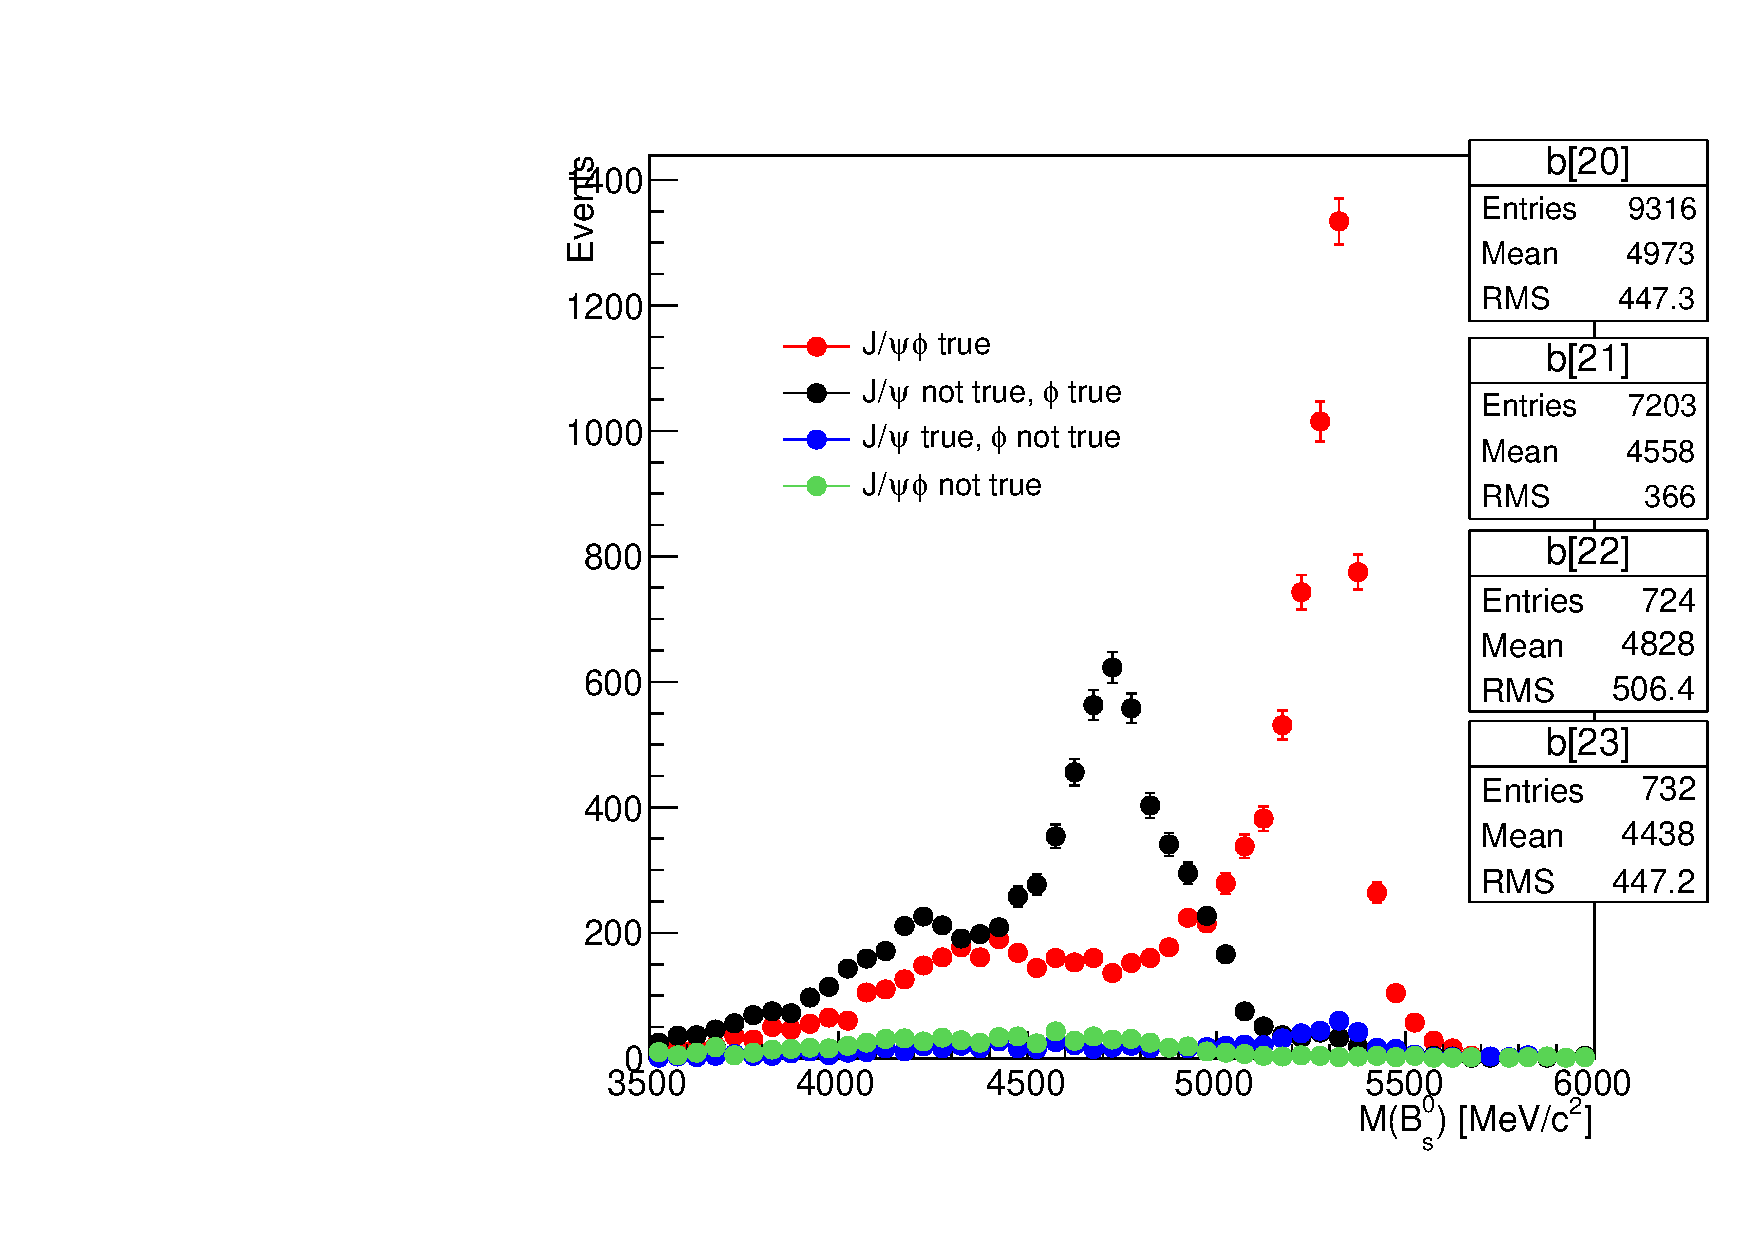
\includegraphics[width=0.52\linewidth]{Bkg2_BsDTF/Bs_M_Bs2JpsieeX_divideBkg_fullrange_newcuts.pdf}\put(-115,-4){(a)}
    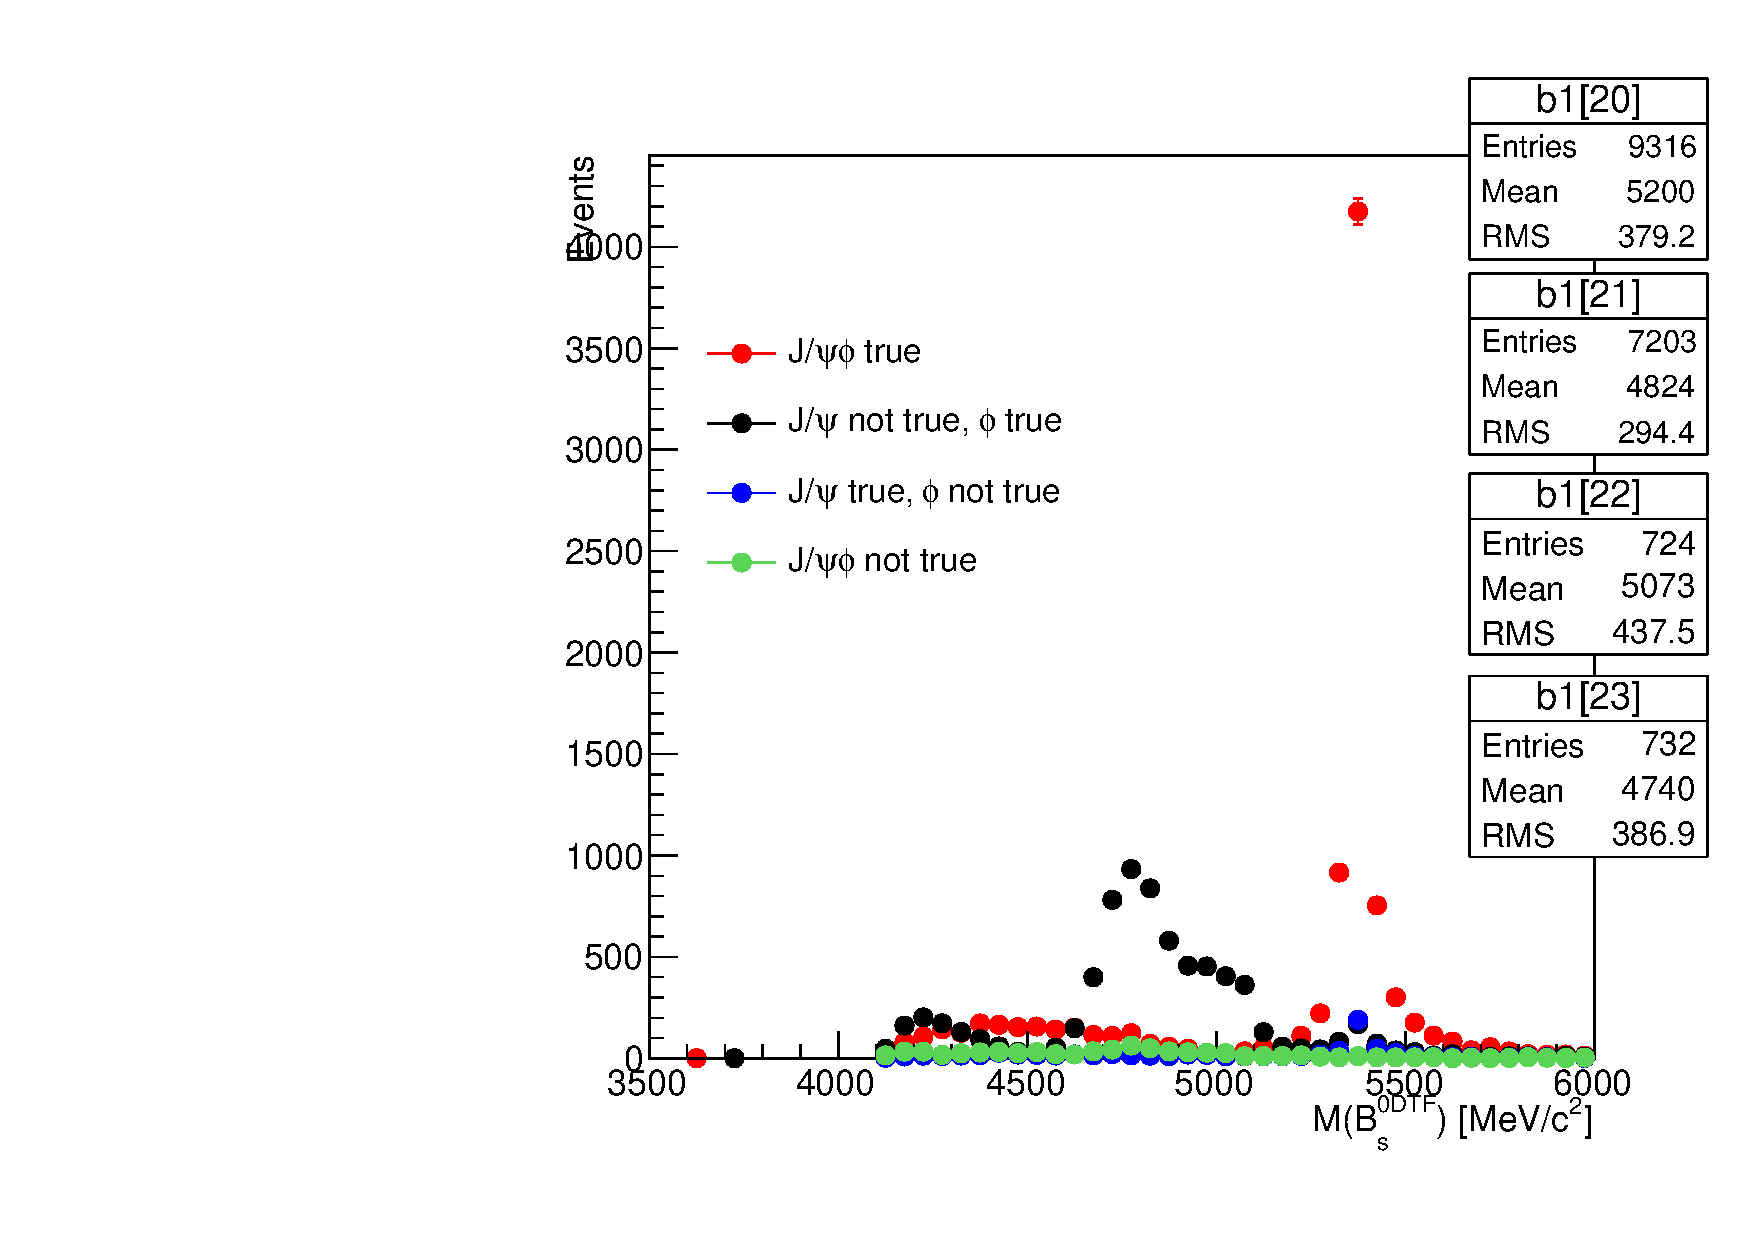
\includegraphics[width=0.52\linewidth]{Bkg2_BsDTF/BsDTF_M_Bs2JpsieeX_divideBkg_fullrange_newcuts.pdf}\put(-115,-4){(b)}
  \end{center}
  \caption{
   The background from partially reconstructed events due to missing particles from the $\jpsi$ and/or hadronic part: (a) $\Bs$ mass distribution, (b) $\Bs$ mass distribution using DTF.
}
  \label{fig:PartReconBkg}
\end{figure}
\begin{figure}[htb]
  \begin{center}
    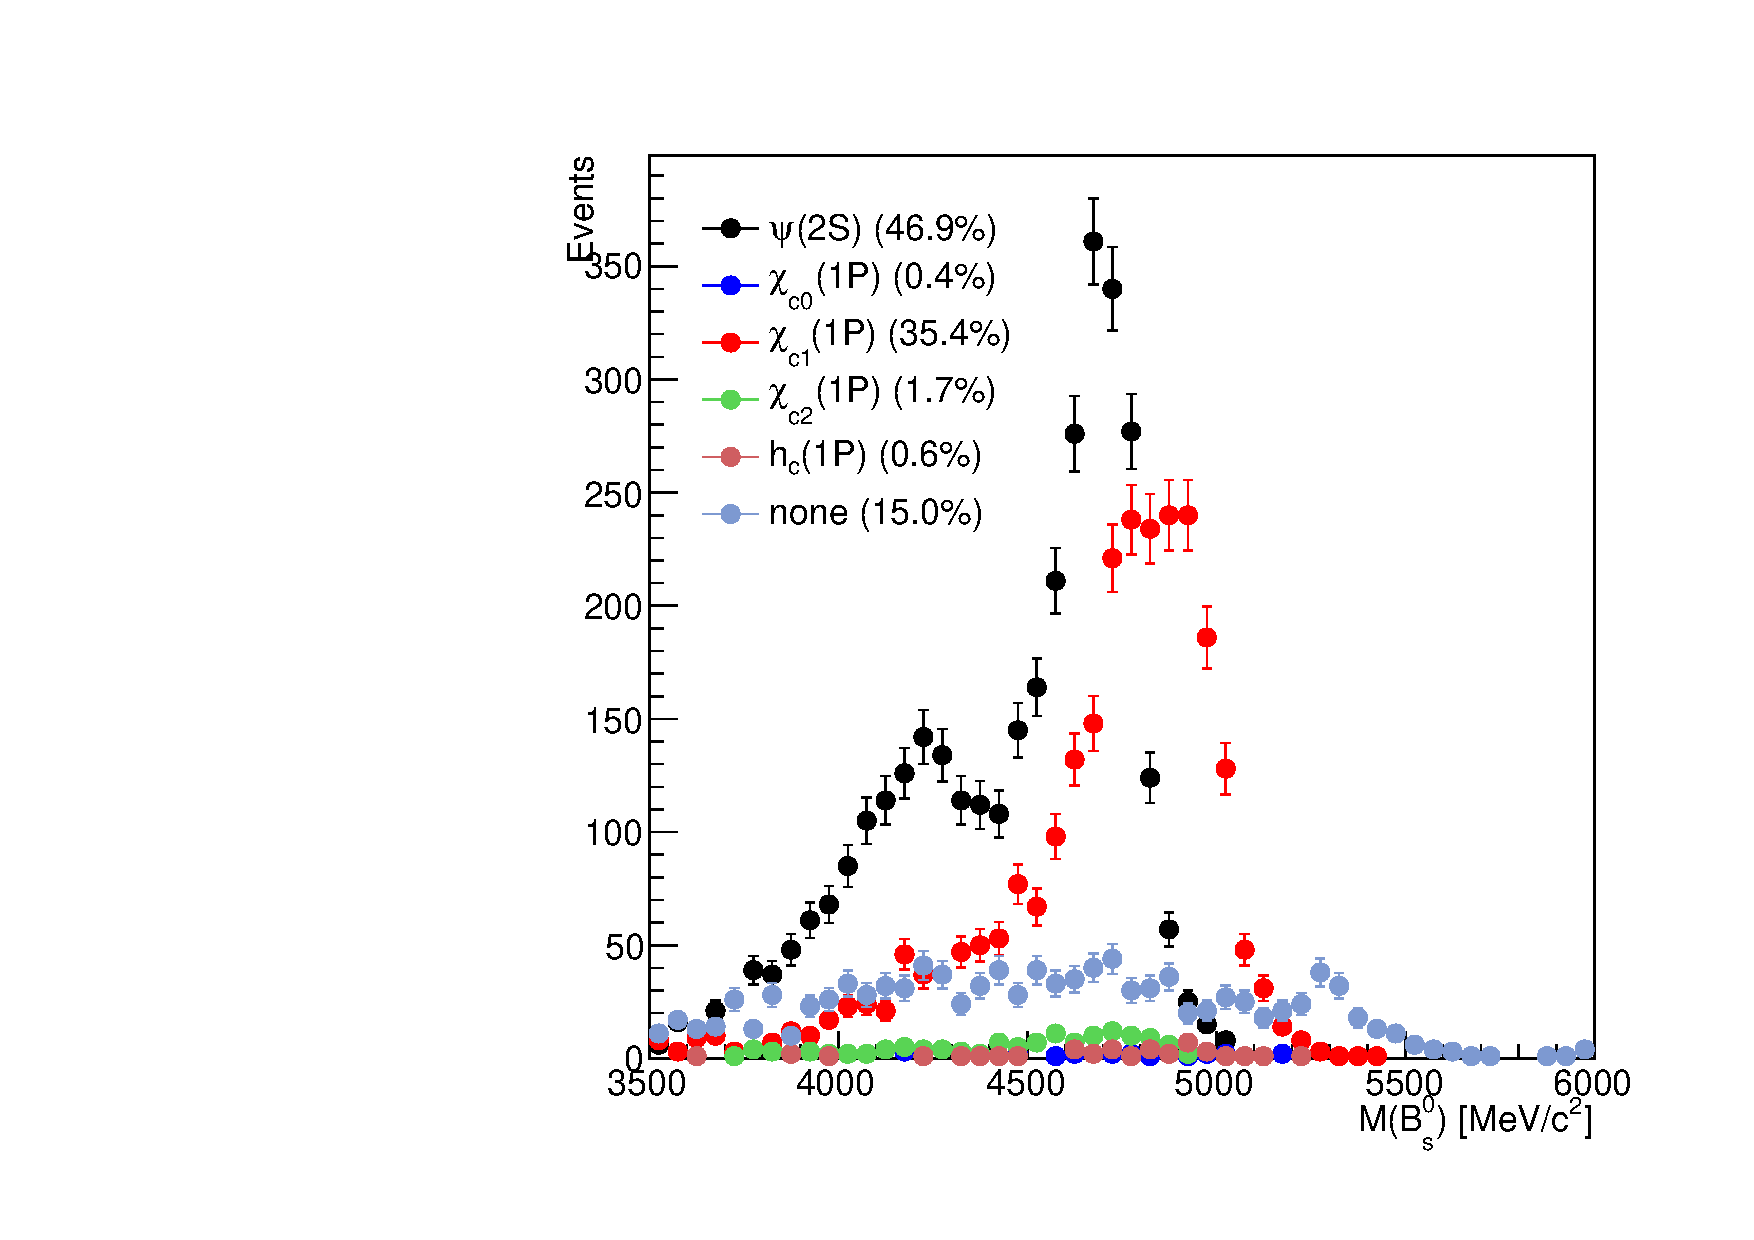
\includegraphics[width=0.52\linewidth]{Bkg2_BsDTF/Bs_M_Bs2JpsieeX_JpsiBkg_fullrange_newcuts.pdf}\put(-115,-4){(a)}
    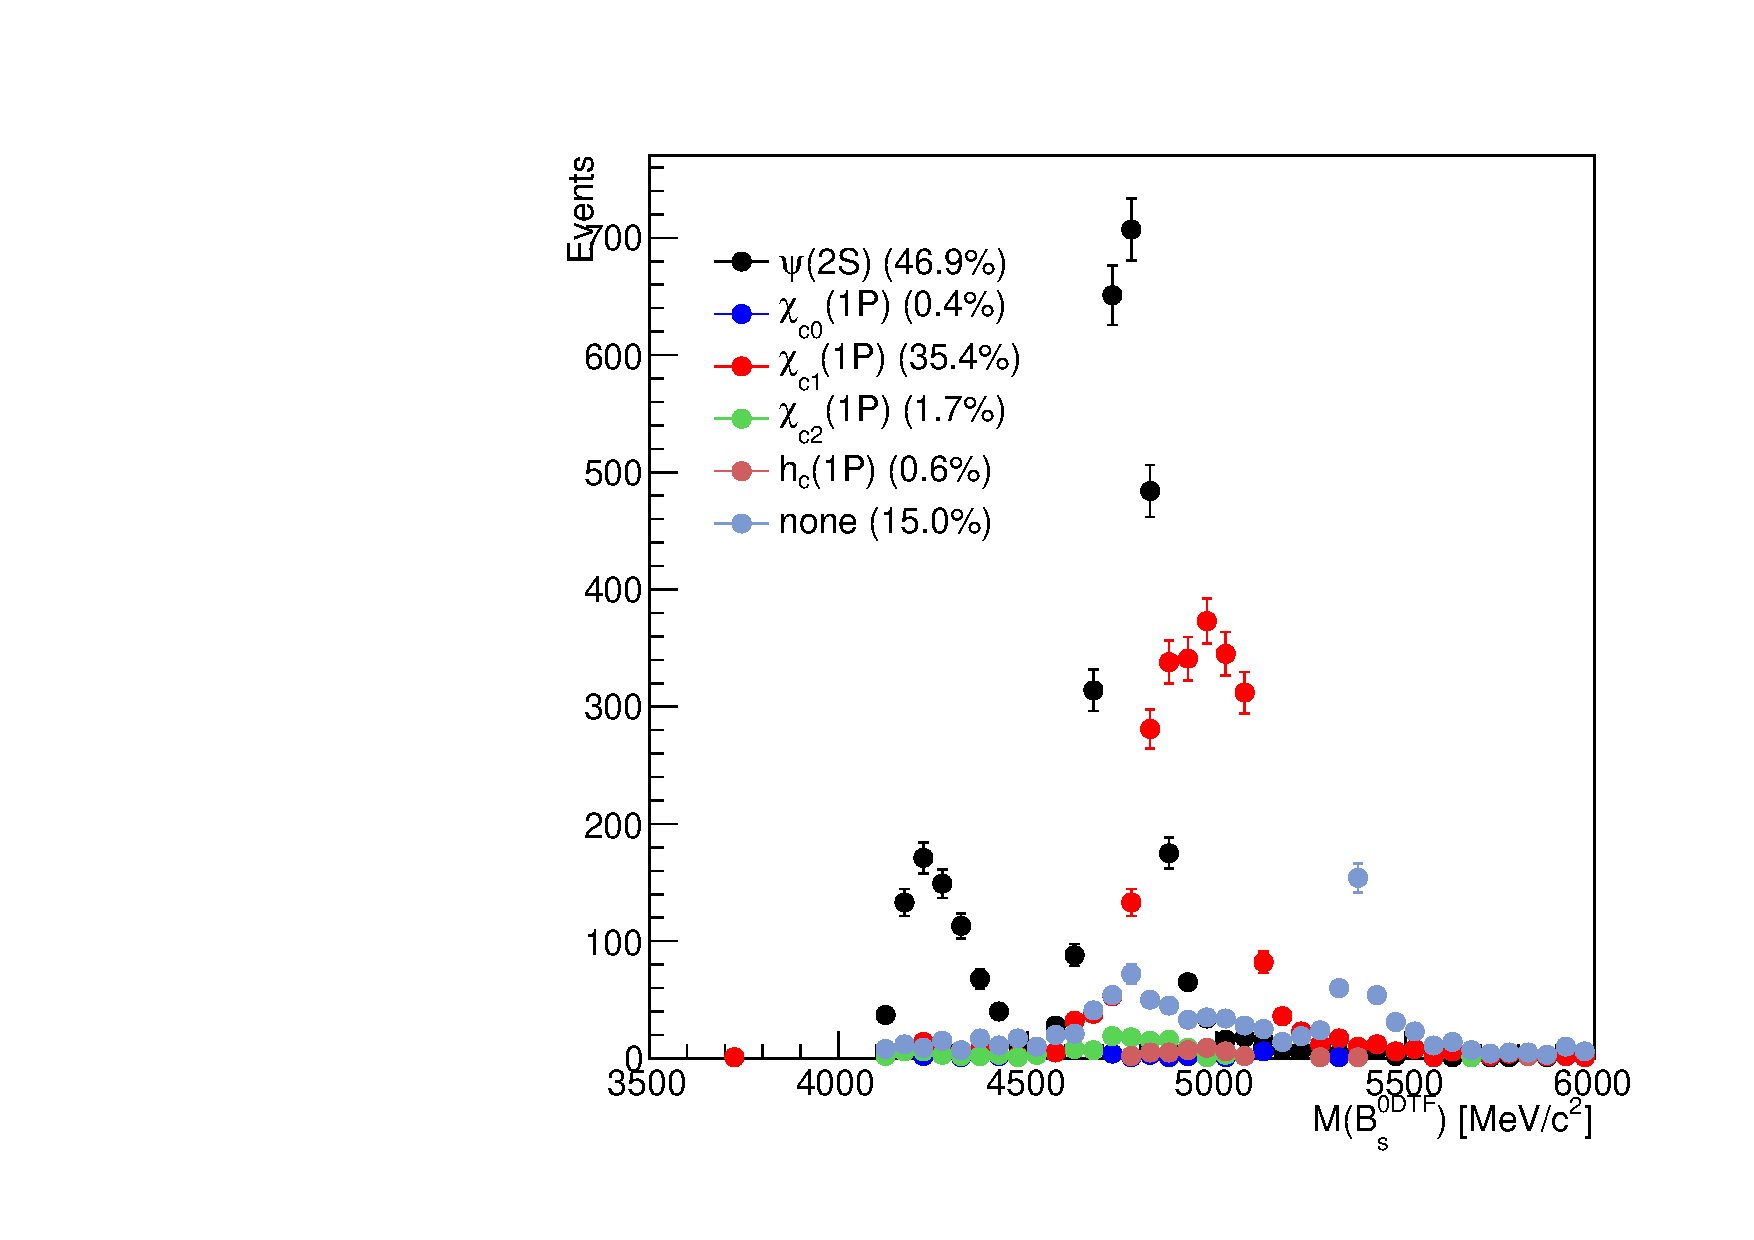
\includegraphics[width=0.52\linewidth]{Bkg2_BsDTF/BsDTF_M_Bs2JpsieeX_JpsiBkg_fullrange_newcuts.pdf}\put(-115,-4){(b)}
  \end{center}
  \caption{
   The $\jpsi$ partially reconstructed background from the excited charmonium resonances for (a) $\Bs$ mass distribution and (b) $\Bs$ mass distribution using DTF.
}
  \label{fig:PartReconBkg_Jpsi}
\end{figure}
\clearpage

\section{Decay time resolution}\label{sec:TimeRes}

The precision of the $\phis$ determination is dependent on the decay time resolution. As in the $\Bs\to\jpsi(\mumu)\Kp\Km$ analysis~\cite{Aaij:2014-039} it could be determined from a sample of prompt $\jpsi\to\epem$ events selected using the following decay time stripping and unbiased trigger lines:
\begin{itemize}
 \item Stripping line: {\tt StrippingBs2JpsieePhiLine}
 \item Unbiased triggers: {\tt L0ElectronDecision$\_$TOS} or {\tt L0HadronDecision$\_$TOS}
\end{itemize}
However, no $\jpsi\to\epem$ peak is observed in the data (Fig.~\ref{fig:JpsiPeak}a), even after testing different criteria to try and isolate the signal. The $\jpsi$ peak arises using a constraint $\Bs$ decay time $t>0.3$~$\ps$ (Fig.~\ref{fig:JpsiPeak}b). 
\begin{figure}[htb]
  \begin{center}
    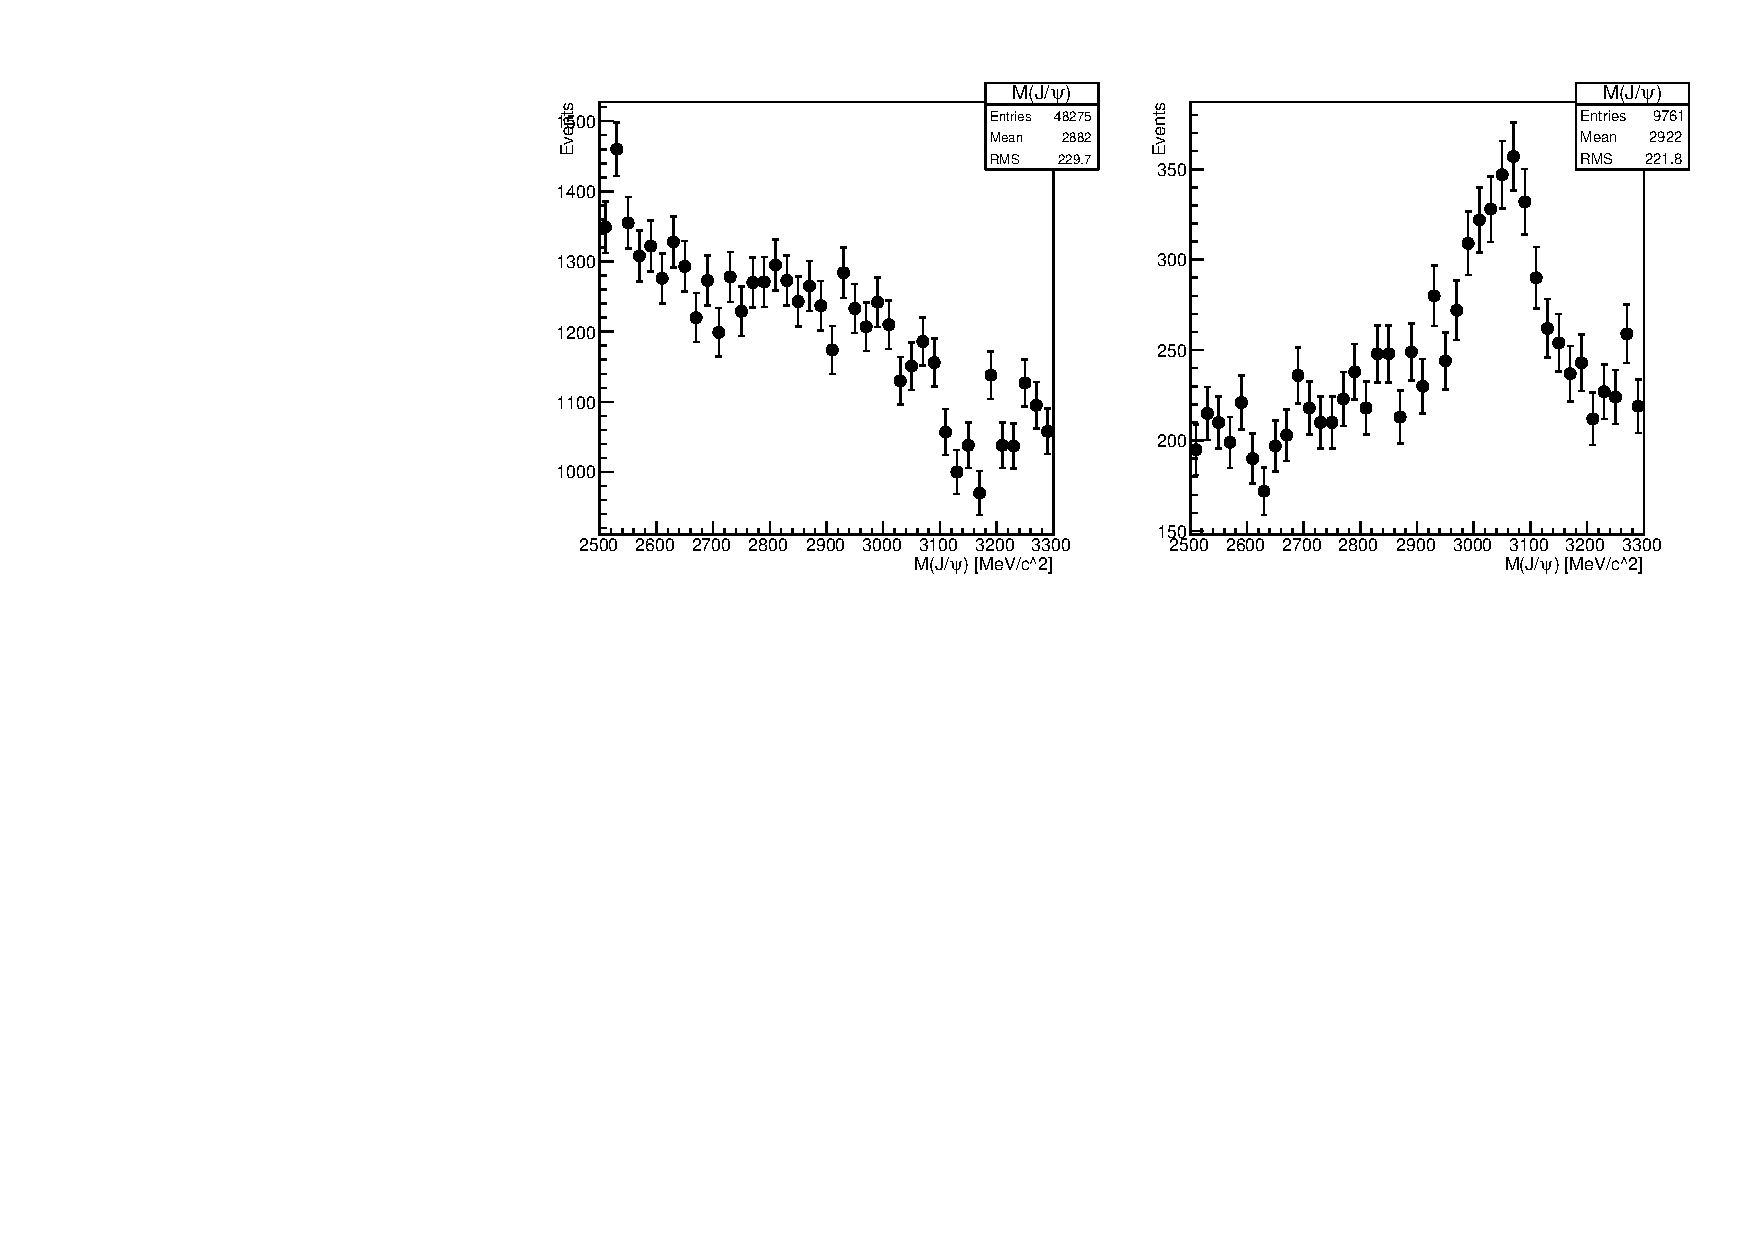
\includegraphics[width=0.9\linewidth]{TimeRes/Jpsi_M_allcuts_time03ps.pdf}\put(-315,-4){(a)} \put(-110,-4){(b)}
  \end{center}
  \caption{
   (a) The distribution of the $\jpsi\to\epem$ invariant mass for events selected using the {\tt Bs2JpsieePhiLine} stripping line with unbiased {\tt L0ElectronDecision$\_$TOS} and {\tt L0HadronDecision$\_$TOS} triggers. No clear sign of the $\jpsi\to\epem$ decays is visible. (b) The distribution of the $\jpsi\to\epem$ invariant mass for events selected using in addition the cut on the $\Bs$ decay time $t>0.3$~$\ps$. The peak from $\jpsi\to\epem$ decays is seen. 
}
  \label{fig:JpsiPeak}
\end{figure}

To solve this problem we compare the time resolution of the $\epem$ and $\mumu$ modes of the $\Bs\to\jpsi\phi$ decays, as the kinematics of these two modes are similar (see Appendix~\ref{sec:app:Comparison}). To do this the simulated signal events from the $\Bs\to\jpsi(\epem)\phi$ and $\Bs\to\jpsi(\mumu)\Kp\Km$ channels are used. A fit was performed to the difference between the true and reconstructed decay time for unbiased 2012 simulated events for both modes using the triple Gaussian resolution model. The $\Bs\to\jpsi(\epem)\phi$ unbiased events pass {\tt L0ElectronDecision$\_$TOS} or {\tt L0HadronDecision$\_$TOS} triggers. In case of the $\Bs\to\jpsi(\mumu)\Kp\Km$ decay, the unbiased sample includes events which passed {\tt Hlt2DiMuonDetachedJPsi$\_$TOS} and {\tt Hlt1DiMuonHighMass$\_$TOS} trigger lines. The parameters resulting from the fit are presented in Table~\ref{tab:TimeRes}. No sizable difference between the two modes is visible. Plots showing the fit to the difference in true and reconstructed decay time are depicted in Fig.~\ref{fig:TimeResMC12}. The time resolution of the $\Bs\to\jpsi(\epem)\phi$ decay is comparable with the time resolution of the $\Bs\to\jpsi(\mumu)\Kp\Km$ decay mode.
\begin{figure}[htb]
  \begin{center}
    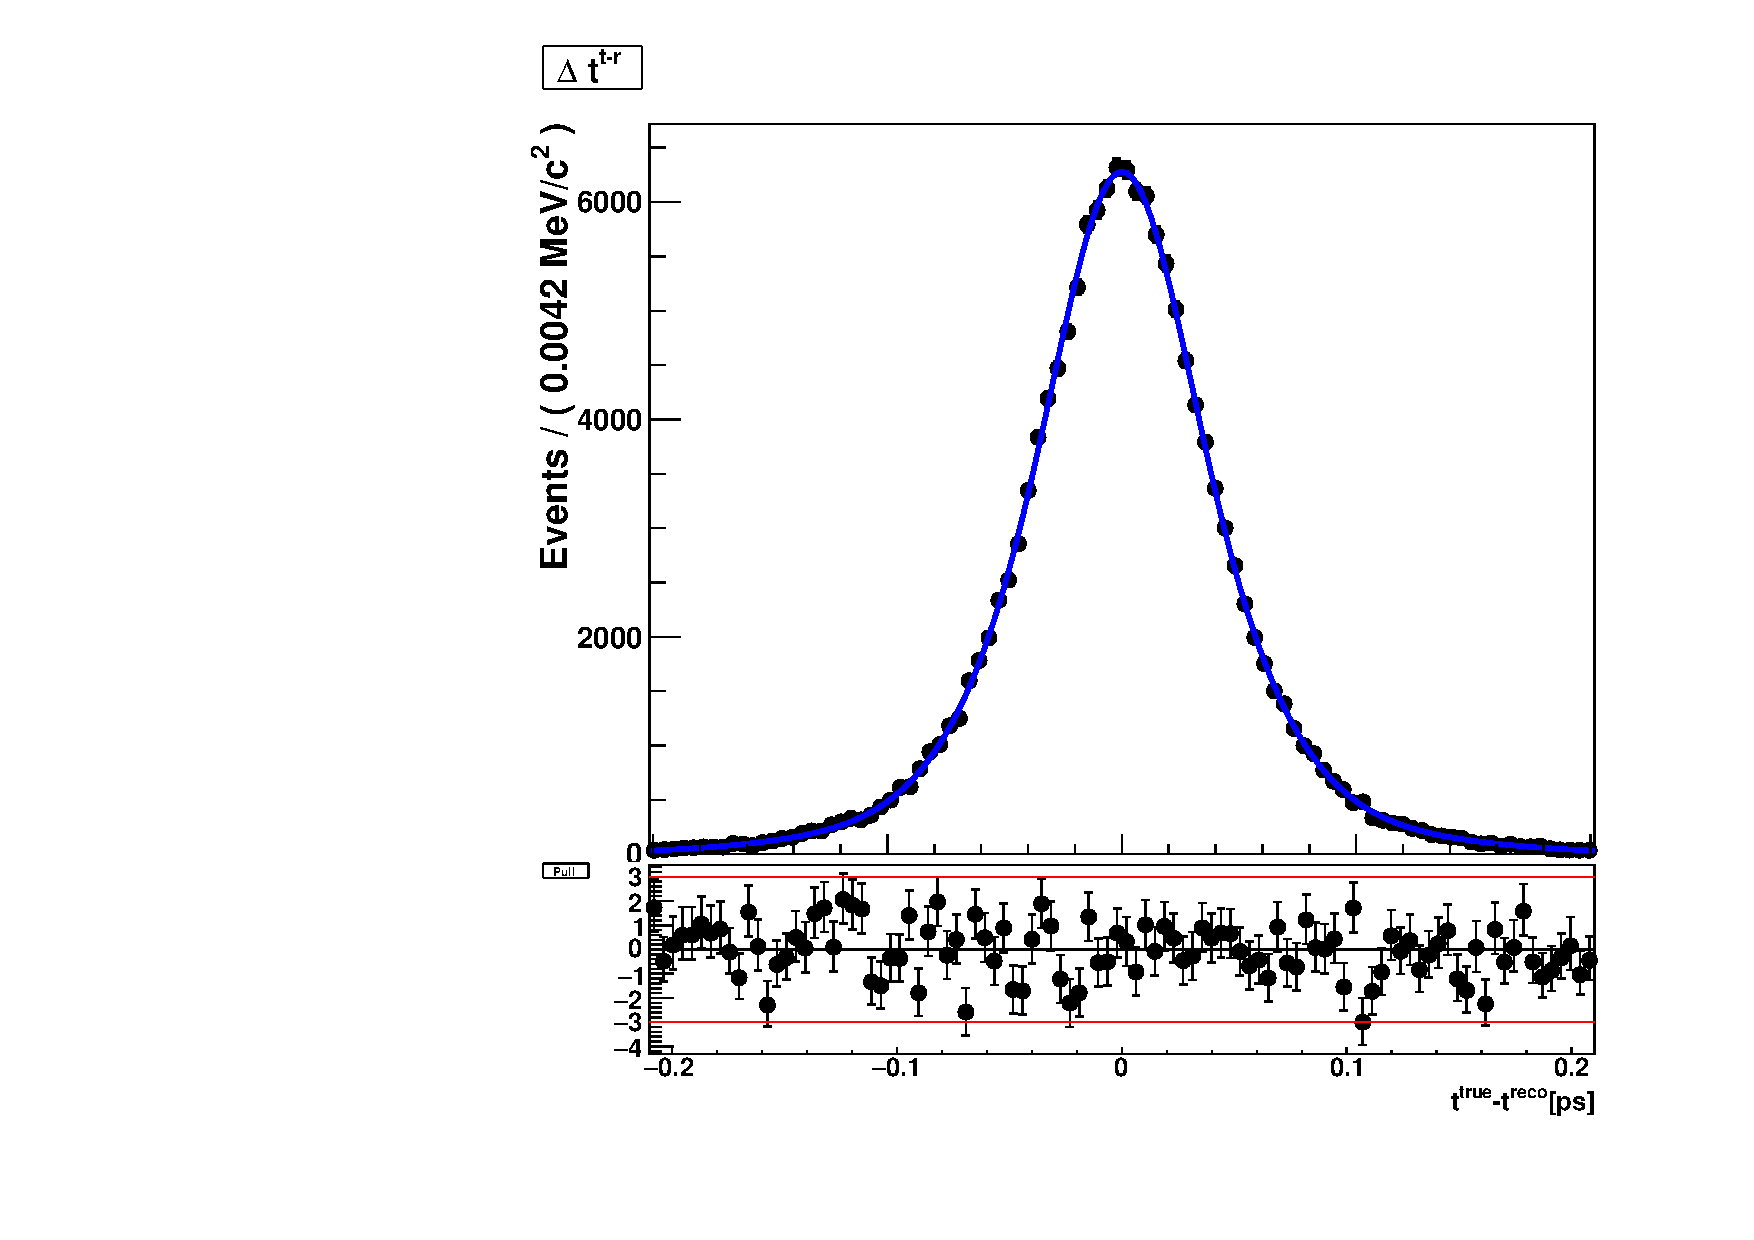
\includegraphics[width=0.49\linewidth]{TimeRes/time_diff_ps_MC12_unbias_pull.pdf}\put(-115,-4){(a)} 
    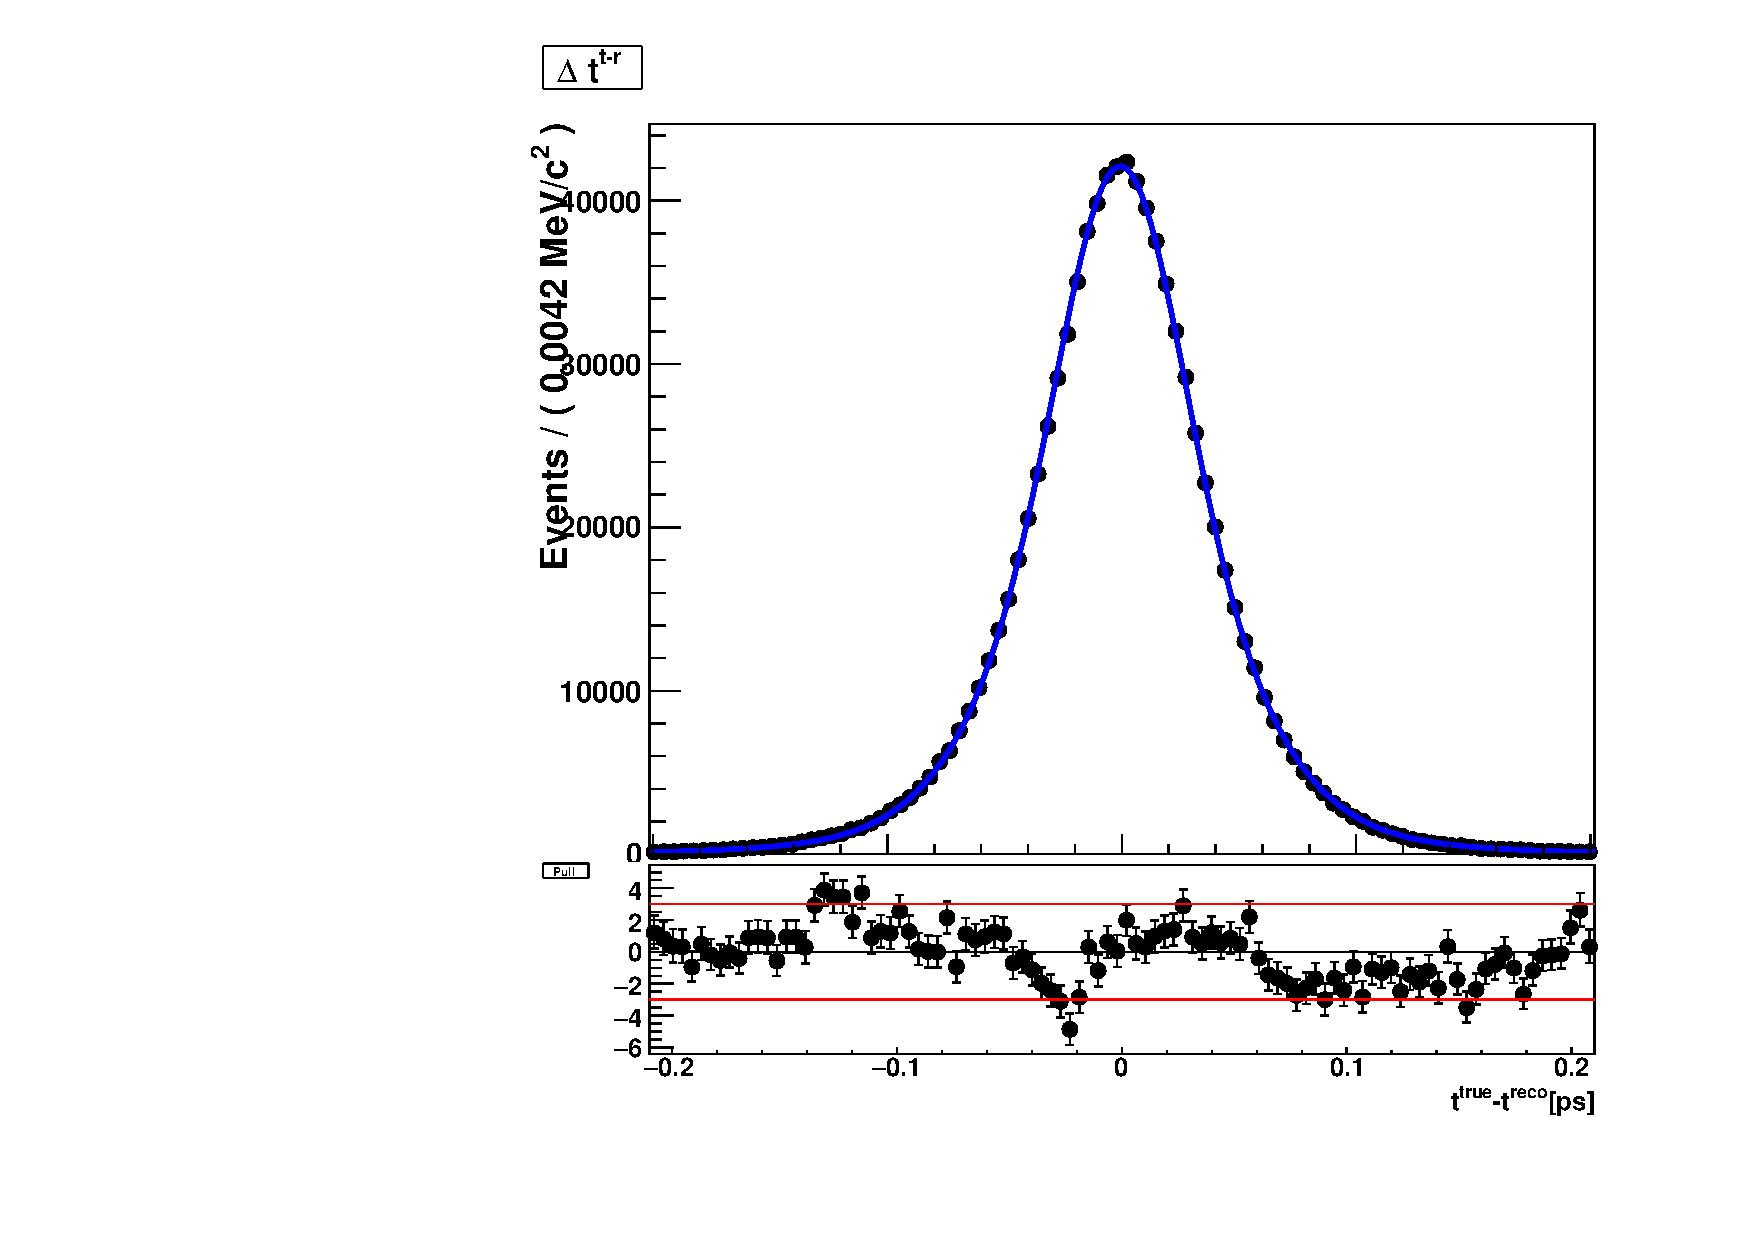
\includegraphics[width=0.49\linewidth]{TimeRes/time_diff_ps_MC12_Bs2JpsiMuMuPhi_unbias_pull.pdf}\put(-115,-4){(b)}
  \end{center}
  \caption{
   The distribution of $t = t^{true} - t^{reco}$ of 2012 simulated (a) $\Bs\to\jpsi(\epem)\phi$ and (b) $\Bs\to\jpsi(\mumu)\Kp\Km$ data samples. The solid blue line shows the result of a fit of the triple Gaussian resolution model. The black points with error bars represent data.
}
  \label{fig:TimeResMC12}
\end{figure}
\begin{table}[htb]
  \caption{
    The resolution model parameters obtained from a fit to the difference between the true and reconstructed decay time using 2012 simulated $\Bs\to\jpsi(\epem)\phi$ and $\Bs\to\jpsi(\mumu)\Kp\Km$ data samples.
}
\small{
\begin{center} \begin{tabular}{ccc}
    \hline
    & $\Bs\to\jpsi(\epem)\phi$ & $\Bs\to\jpsi(\mumu)\Kp\Km$  \\
    \hline
   $\mu_{\text{Gaussians}}$~[$\ps$] & 0.00010$\pm$0.00012 & -0.000656$\pm$0.00004  \\
   $\sigma_{1}$~[$\ps$]& 0.0836$\pm$0.0022 & 0.0249$\pm$0.0004  \\
   $\sigma_{2}$~[$\ps$]& 0.0243$\pm$0.0017 & 0.0871$\pm$0.0017 \\
   $\sigma_{3}$~[$\ps$]& 0.0416$\pm$0.0016 & 0.0437$\pm$0.0006 \\
   f$_{1}$ & 0.194$\pm$0.018 & 0.340$\pm$0.017 \\
   f$_{2}$ & 0.207$\pm$0.053 & 0.099$\pm$0.007 \\
   f$_{3}$ & 0.599$\pm$0.050 & 0.561$\pm$0.017 \\
   \hline
   $\sigma_{eff}$~[ps] & 0.0502$\pm$0.0019 & 0.0451$\pm$0.0008  \\
  \hline
    \end{tabular}\end{center}
  }
\label{tab:TimeRes}
\end{table}
\clearpage

\section{Decay time acceptance}\label{sec:TimeAcc}

 As the decay time is used in the log-likelihood fit to data, it is necessary to model the acceptance effects of the detector and selection process. To perform this we use the data driven {\tt TISTOS} method to determine the trigger efficiencies in data and simulation. The detailed procedure of the {\tt TISTOS} method is described in Ref.~\cite{LHCb:PUB-2014-039} but the main concept is repeated in this paper. 
 
 In the LHCb, the efficiency (conventionally) is a product of three terms:
 \begin{equation}
  \epsilon_{tot} = \epsilon_{rec|acc}\cdot\epsilon_{sel|rec}\cdot\epsilon_{trig|sel},
 \end{equation}
 where the particles in the candidate events must first lie within the detector acceptance, then be reconstructed, selected, and finally passed the trigger requirements. The trigger efficiency is defined on the final sample of selected events:
 \begin{equation}\label{eq:TrigEff}
  \epsilon_{trig}\equiv\epsilon_{trig|sel}\equiv\frac{N_{trig}}{N_{sel}}.
 \end{equation}
 To estimate the trigger efficiency (Eq.~\ref{eq:TrigEff}) from the data, the events are splitted into two trigger categories:
 \begin{itemize}
  \item Triggered On Signal (TOS): events for which the presence of the signal is sufficient to generate a positive trigger decision;
  \item Triggered Independent of Signal (TIS): the "rest" of the events is sufficient to generate a positive trigger decision, where the rest of the event is defined through an operational procedure consisting in removing the signal and all detector hits beloning to it.
 \end{itemize}
A single event can be also simultaneously TIS and TOS (TISTOS). If both the presence of the signal alone as well as the rest of the event alone are sufficient to generate a positive trigger decision. Using these event categories, the partial efficiencies are defined as
\begin{equation}\label{eq:PartTrigEff}
 \epsilon_{TOS}\equiv\frac{N_{TOS}}{N_{sel}},\qquad\epsilon_{TIS}\equiv\frac{N_{TIS}}{N_{sel}},\qquad\epsilon_{TISTOS}\equiv\frac{N_{TISTOS}}{N_{sel}}.
\end{equation}

Since the trigger efficiency (Eq.~\ref{eq:TrigEff}) can be expressed using the trigger categories (Eq.~\ref{eq:PartTrigEff}), we express $\epsilon_{trig}$ as follows:
\begin{equation}
 \epsilon_{trig}=\frac{N_{trig}}{N_{sel}}=\frac{N_{trig}}{N_{TIS}}\times\frac{N_{TIS}}{N_{sel}}=\frac{N_{trig}}{N_{TIS}}\times\epsilon_{TIS}.
\end{equation}
That the TIS efficiency of any subsample of the triggered events is the same as that of the whole sample of selected events, it can thus be measured on the TOS sample:
\begin{equation}
 \epsilon_{TIS}\equiv\epsilon_{TIS|TOS}.
\end{equation}
The trigger efficiency can now be expressed as
\begin{equation}\label{eq:FinalTrigEff}
 \epsilon_{trig}=\frac{N_{trig}}{N_{TIS}}\times\frac{N_{TISTOS}}{N_{TOS}},
\end{equation}
where all four quantities can be directly measured from data.

 The trigger efficiencies of the $\Bs\to\jpsi\phi$ data and simulated sample are obtained for two trigger categories (described in Sec.~\ref{subsec:Trigger}):
 \begin{enumerate}
  \item Unbiased: {\tt L0ElectronDecision$\_$TOS} or {\tt L0HadronDecision$\_$TOS}
  \item Biased: {\tt Hlt1TrackAllL0Decision$\_$TOS}
 \end{enumerate}
 In case of biased triggers, the one trigger is chosen since it holds a maximum number of selected events in the whole biased category: 98.4$\%$ of data events and 91.3$\%$ of simulated events.
 
 The $\Bs\to\jpsi\phi$ trigger efficiencies for unbiased and biased triggers are shown in Fig.~\ref{fig:TimeAccTISTOS}.
   \begin{figure}[hbt]
  \begin{center}
    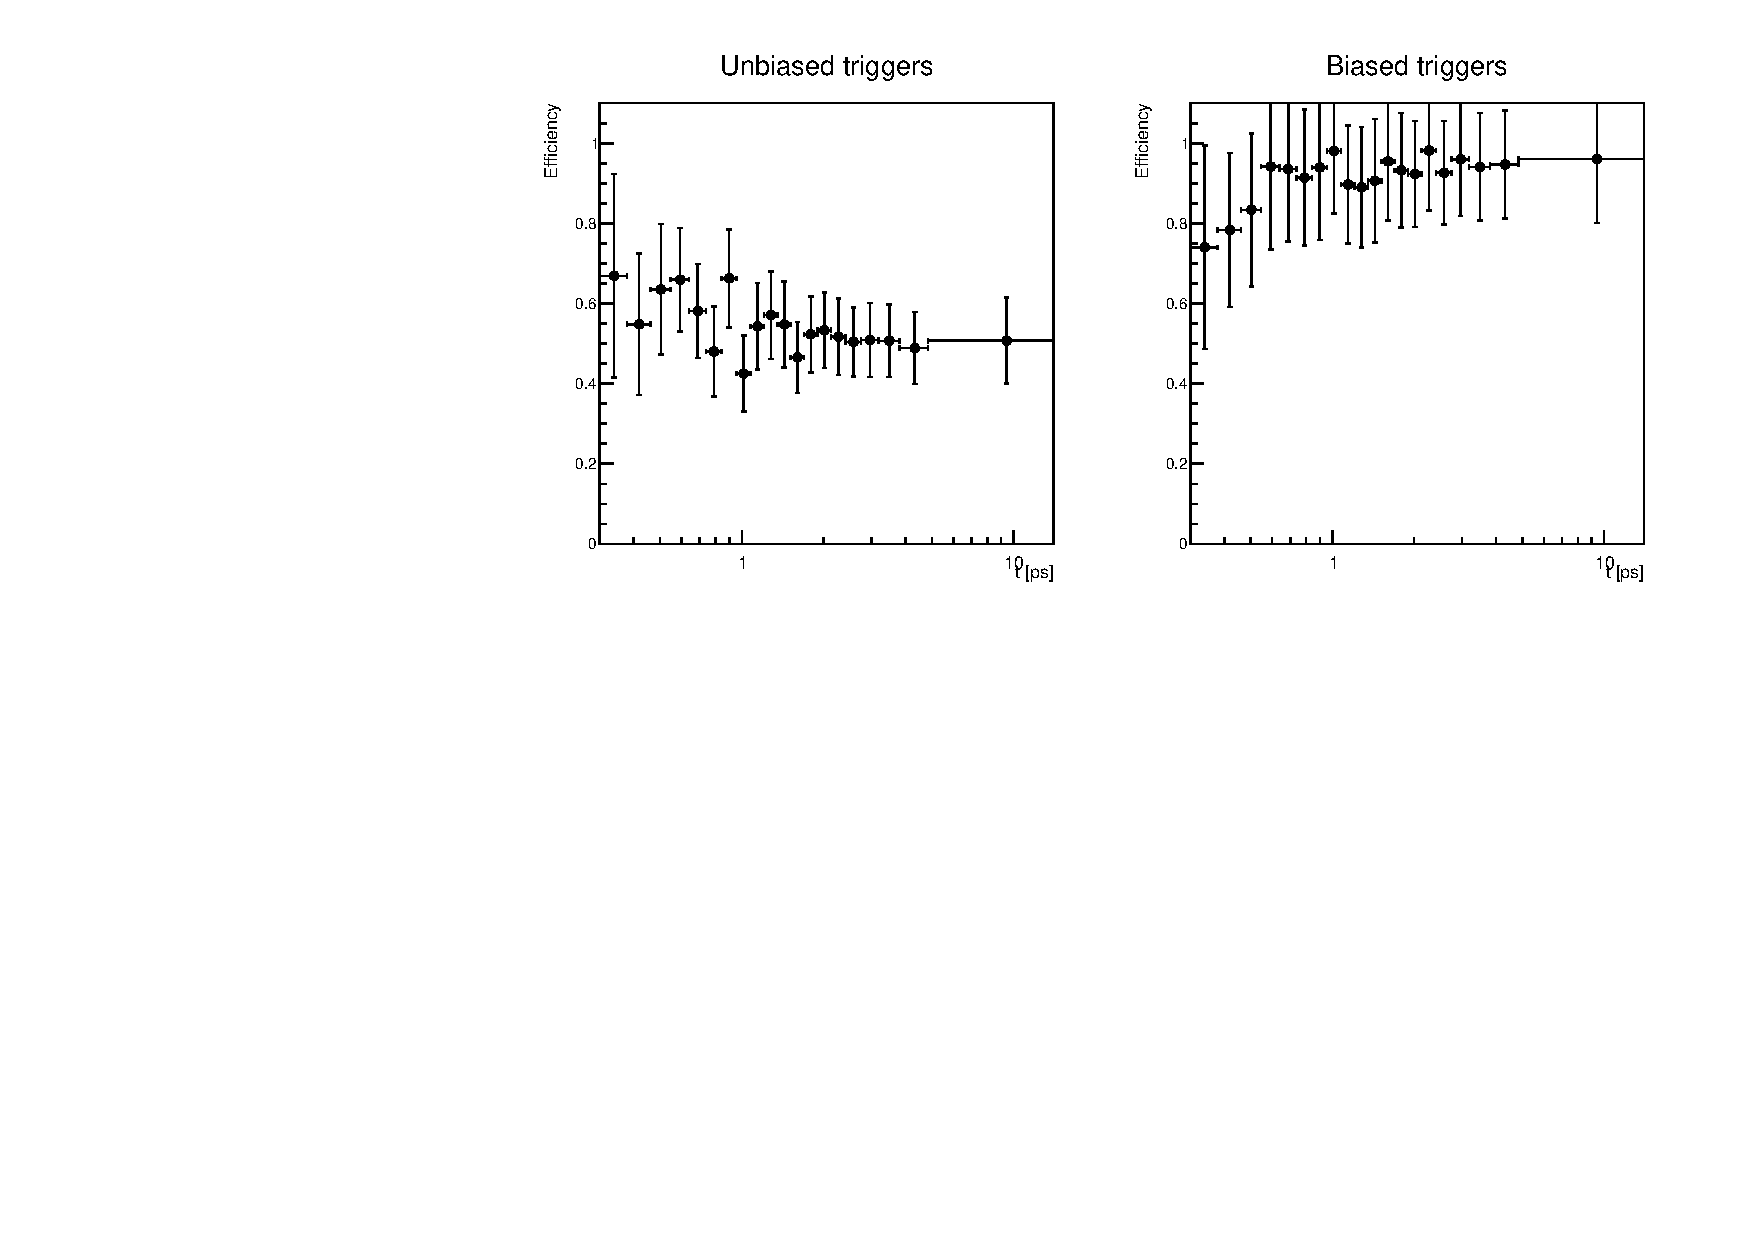
\includegraphics[width=0.9\linewidth]{TimeAcc_TISTOS/Eff_unbL0E_bias_log_data.pdf}\\ 
    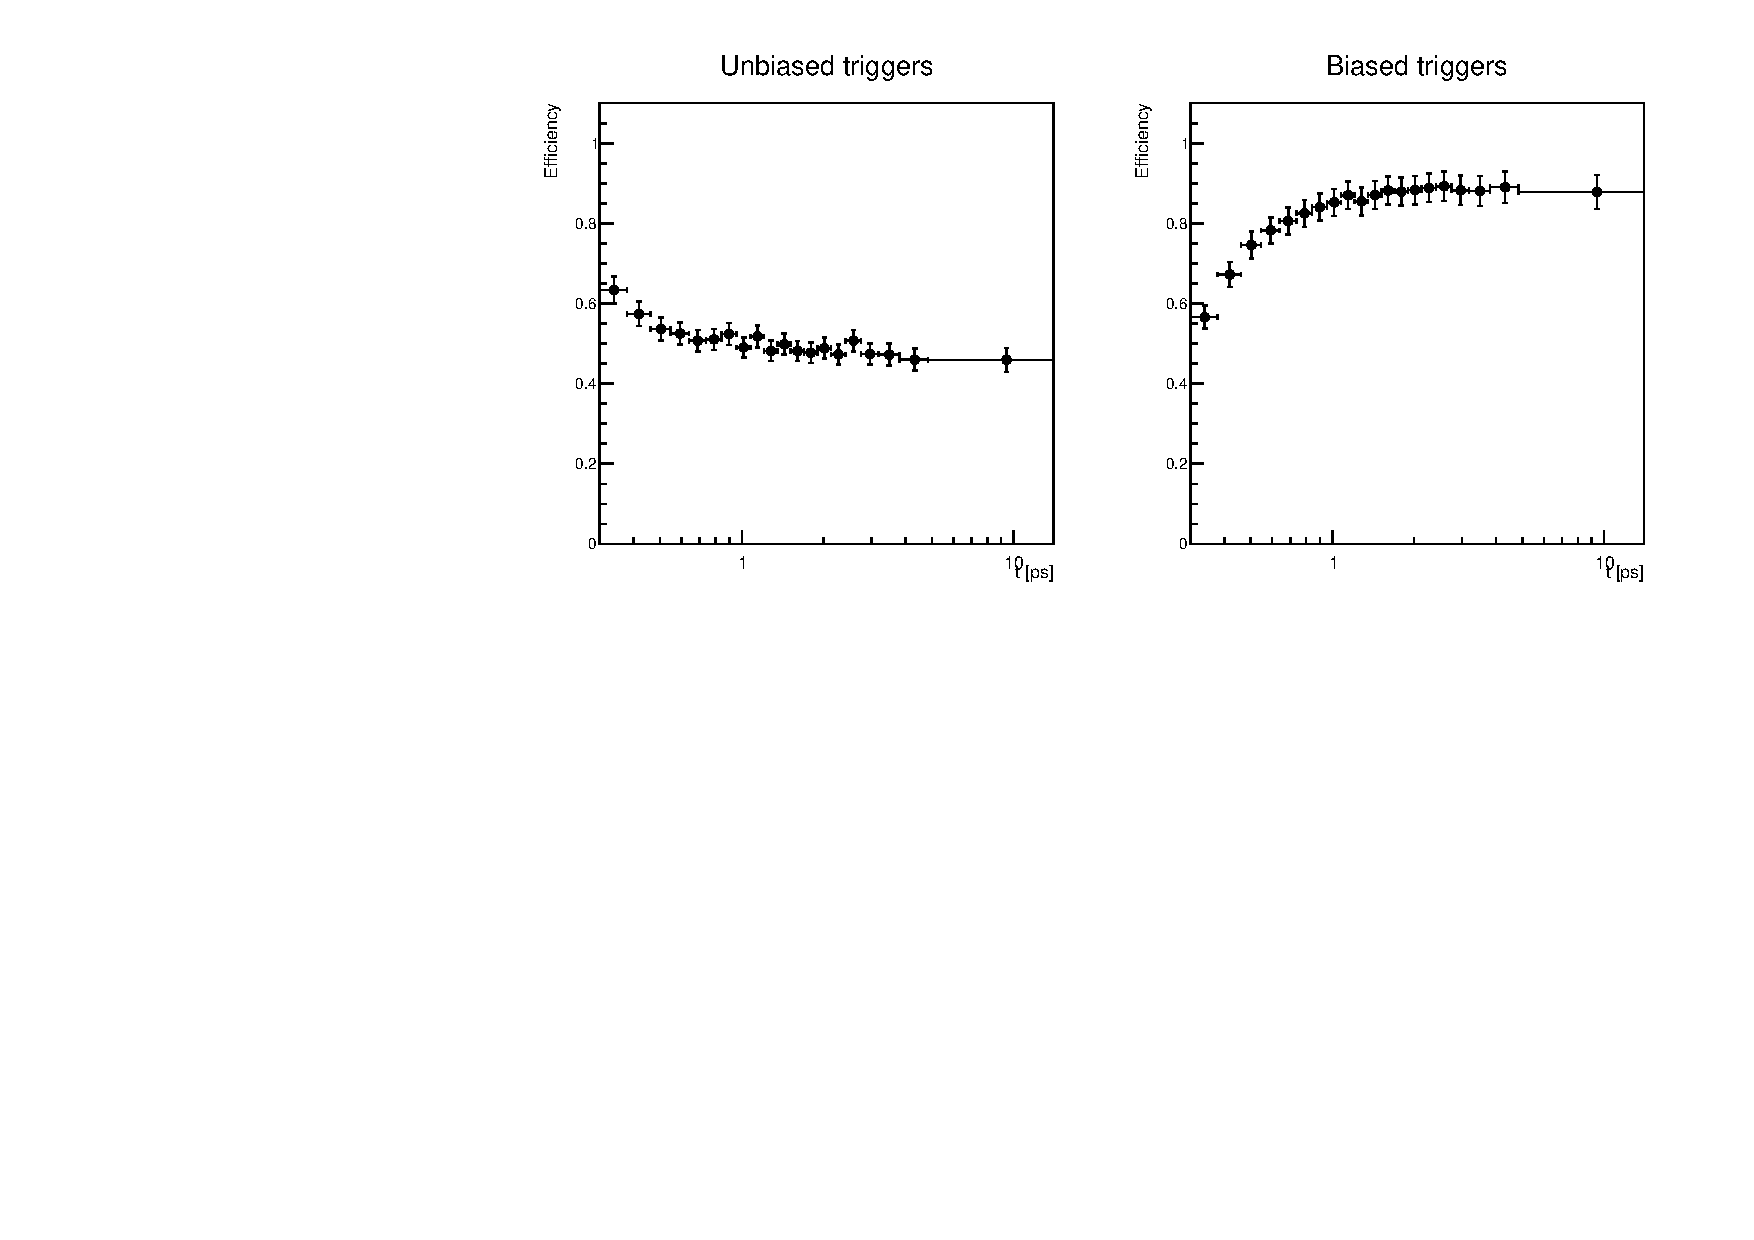
\includegraphics[width=0.9\linewidth]{TimeAcc_TISTOS/Eff_unbL0E_bias_log_MC.pdf}
  \end{center}
  \caption{
  The trigger efficiencies of sWeighted $\Bs\to\jpsi\phi$ data (top) and simulation (bottom) for unbiased (left) and biased (right) triggers depending on the decay time. 
}
  \label{fig:TimeAccTISTOS}
\end{figure}
 
 
 \subsection{Track reconstruction efficiency}\label{subsec:TrackRecEff}
 
 The track reconstruction efficiency is computed as the ratio of the decay time distributions of fully unbiased and truth matched 2012 simulated sample to the toy dataset generated with the 2012 MC physics parameters. The resulting histogram is shown in Fig.~\ref{fig:TimeAccTrackRecEff}. The efficiency ratio is fitted with a quadratic function, $N(1+\beta t+\gamma t^{2})$. The obtained fit parameters of the track reconstruction efficiency for $\Bs\to\jpsi(\epem)\phi$ and $\Bs\to\jpsi(\mumu)\Kp\Km$~\cite{Aaij:2014-039} decays are listed in Table~\ref{tab:TRackRecEff}.
 
  \begin{figure}[hbt]
  \begin{center}
    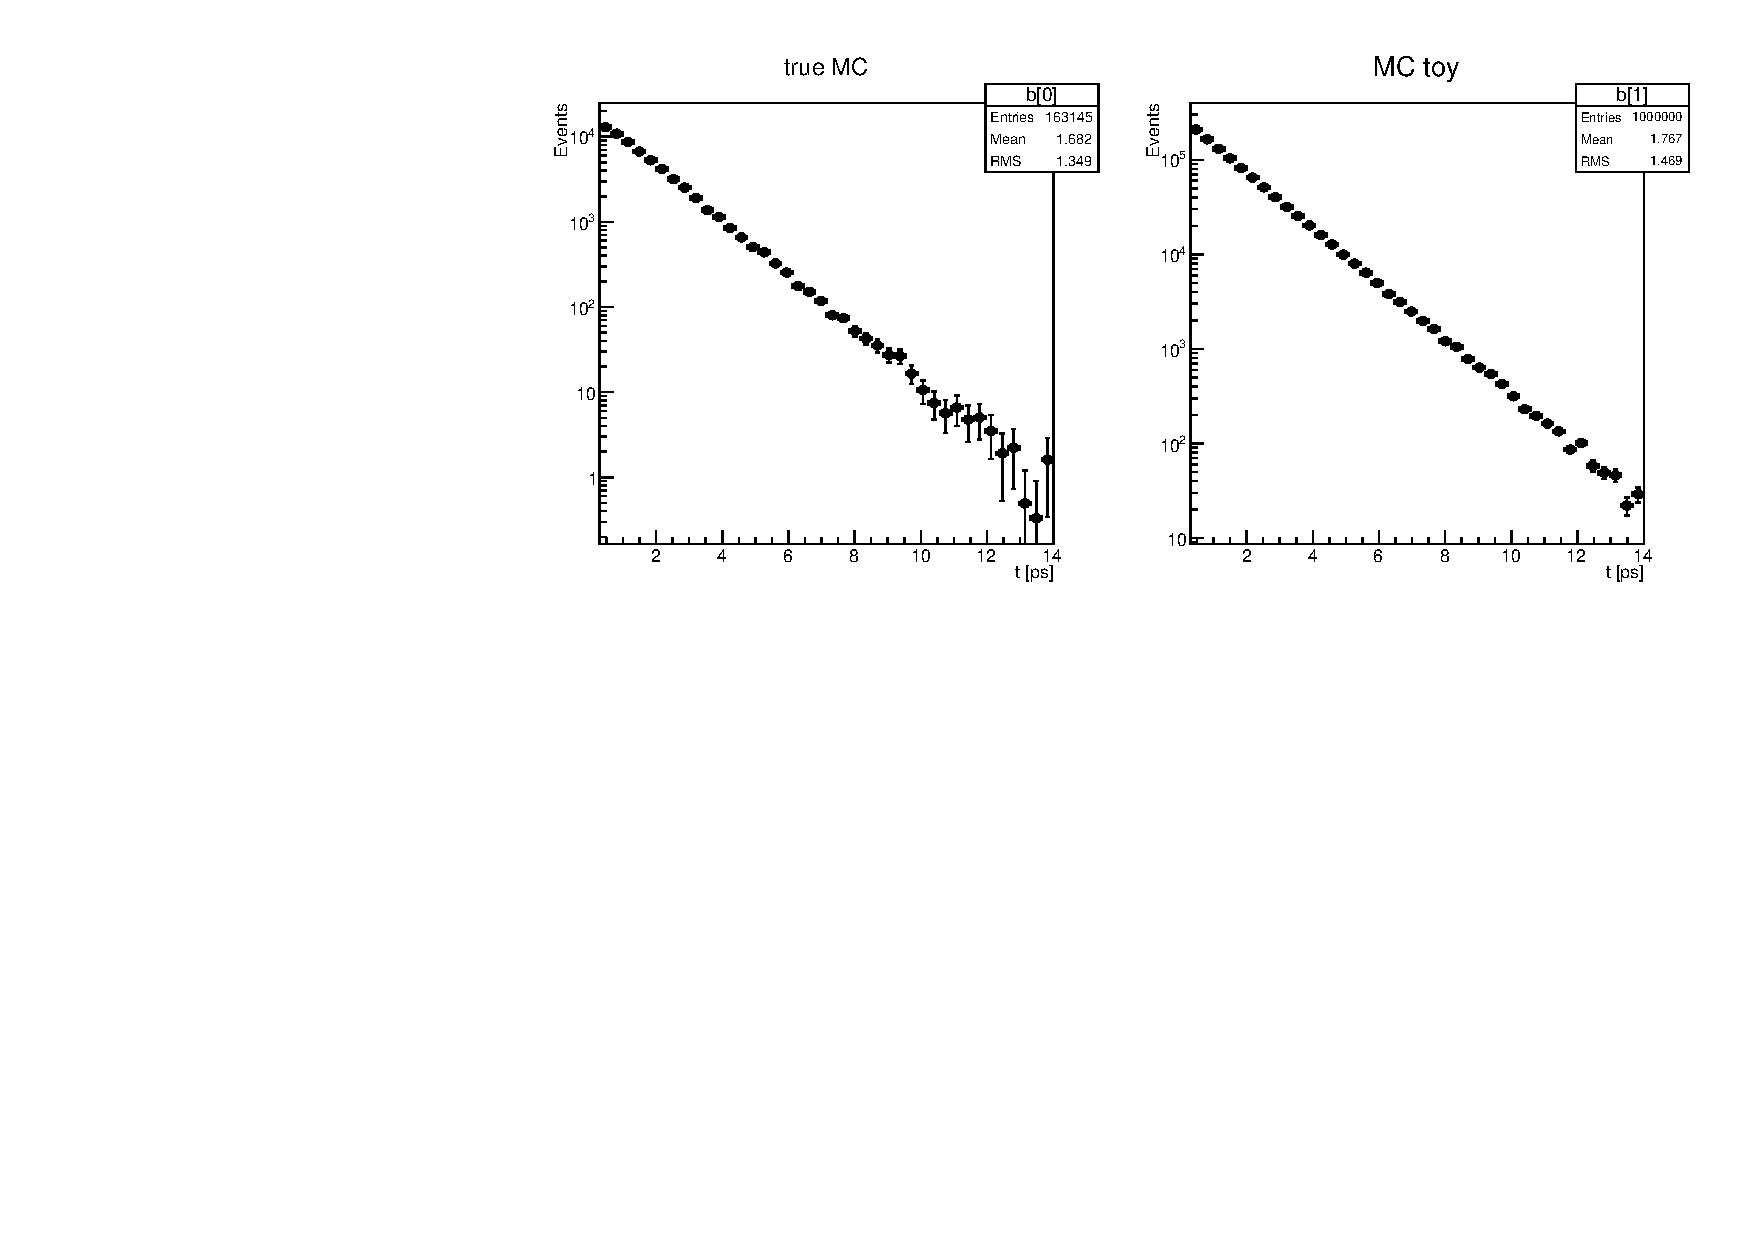
\includegraphics[width=0.9\linewidth]{TimeAcc_high/Time_MCtrue_MCtoy.pdf}\\ 
    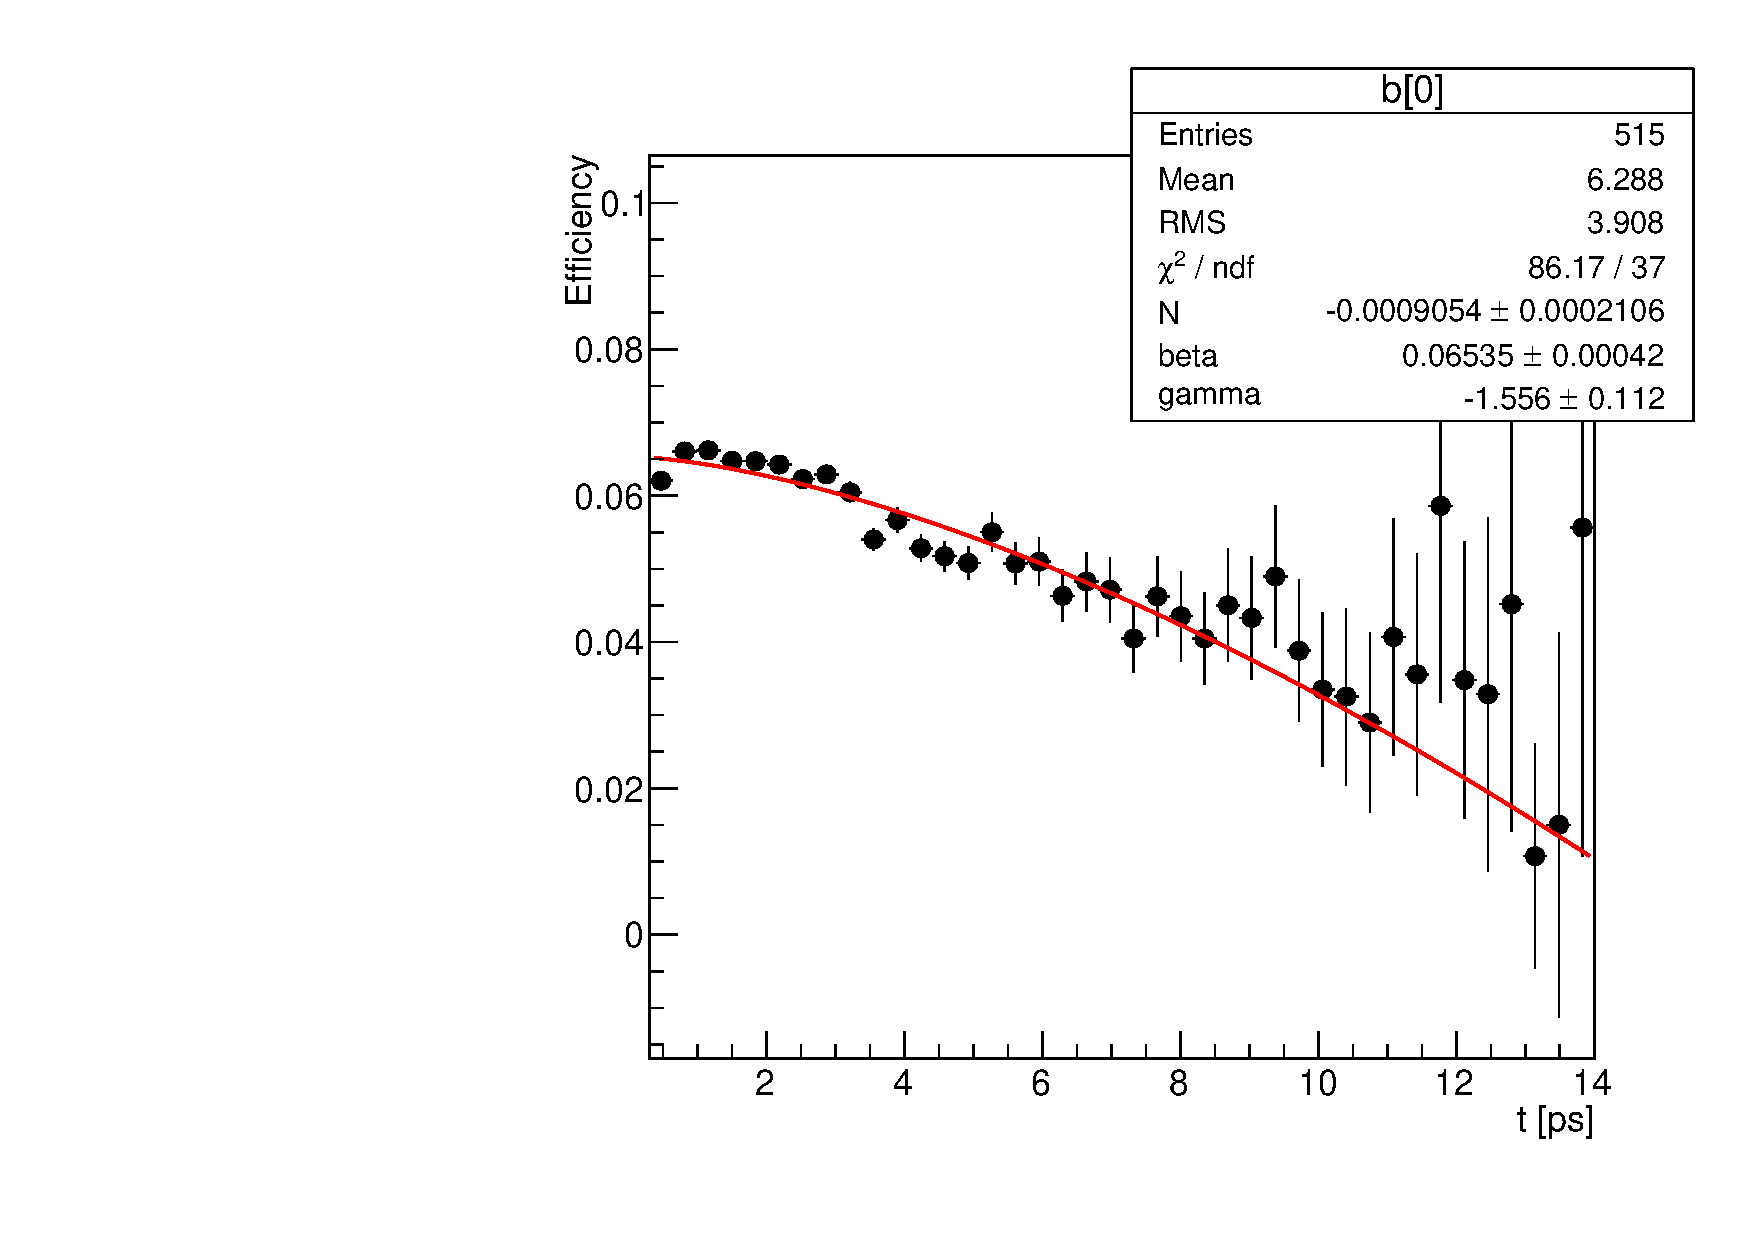
\includegraphics[width=0.45\linewidth]{TimeAcc_high/Efficiency.pdf}
  \end{center}
  \caption{
  The ratio (bottom) of decay time distributions of completely unbiased and truth matched events in 2012 MC (top left) to toy events generated with the 2012 MC physics parameters (top right).
}
  \label{fig:TimeAccTrackRecEff}
\end{figure}

\begin{table}[htb]
  \caption{
    The fit parameters of the track reconstruction efficiency for $\Bs\to\jpsi(\epem)\phi$ and $\Bs\to\jpsi(\mumu)\Kp\Km$ decays.}
    \small{
\begin{center}\begin{tabular}{c|c|c}
   \hline
   Parameter & $B^{0}_{s}\rightarrow J/\psi(e^{+}e^{-})\phi$ & $B^{0}_{s}\rightarrow J/\psi(\mu^{+}\mu^{-})K^{+}K^{+}$ \\
  \hline
   $N_{evt}$ & 515 & 8 241\\
   $\mu$ & 6.29 & 6.59\\
   RMS & 3.91 & 3.82\\
   $\chi^{2}$/ndf & 86.17/37 & 50.16/47\\
   N & -0.00091$\pm$0.00021 & 0.09722$\pm$0.00023\\
   $\beta$ & 0.06535$\pm$0.00042 & 0.00320$\pm$0.00183\\
   $\gamma$&-1.556$\pm$0.112 & -0.00227$\pm$0.00025\\
   \hline
    \end{tabular}
   \end{center}
  }
\label{tab:TRackRecEff}
\end{table}
\clearpage

\section{Angular acceptance}\label{sec:AngAcc}

Effects of angular acceptance are modeled with normalization weights (see Ref.~\cite{Aaij:2012-067}, Sec.~3.3). The normalization weights are obtained from fully simulated signal sample from the Sim08 production (Sec.~\ref{subsec:MC}), as described in Sec.~\ref{subsec:NormWeightMC}. 

\subsection{Normalization weights from full simulation}\label{subsec:NormWeightMC}
 The angular acceptance normalization weights determined with the Sim08 Monte Carlo samples are shown in Table~\ref{tab:UnccorrAngAccMCfull}. Table~\ref{tab:UnccorrAngAccMCfullCorrMatrix} shows the correlations between the errors of the weights. In Table~\ref{tab:UnccorrAngAcc} the 10 weights corresponding to 10 terms of the PDF (Eq.~\ref{eq:decayrate}) are split by running year. As no significant difference is observed between the two years (Fig.~\ref{fig:AnglesAccMC11MC12}), the weights are calculated and normalized separately for each running year and then they are combined to the one final set of weights of Table~\ref{tab:UnccorrAngAccMCfull}. The one-dimentional projections of the angular efficiency functions are shown in Fig.~\ref{fig:AnglesAccMCfull}. No reweighting of the final state kinematics has been applied since the $\Bs$ and $K$ momentum and $\Kp\Km$ mass distribution in simulation are observed to well reproduce those in data (Fig.~\ref{fig:AnglesAcc_IterMeth}).


 \begin{table}[htb]
  \caption{
    The uncorrected angular acceptance weights for the sum of 2011 and 2012 Sim08 simulated sample.}
    \small{
\begin{center}\begin{tabular}{ccc}
    \hline
   & k & $\xi_{k}/\xi_{1}$   \\
    \hline
  1 & (00) & 0.9796$\pm$0.0010 \\
  2 & ($\parallel\parallel$) & 1.0206$\pm$0.0012\\
  3 & ($\perp\perp$) & 1.0208$\pm$0.0012\\
  4 & ($\parallel\perp$) & 0.0005$\pm$0.0013\\
  5 & (0$\parallel$) & 0.0007$\pm$0.0009\\
  6 & (0$\perp$) & 0.0014$\pm$0.0009\\
  7 & (SS) & 0.9929$\pm$0.0008\\
  8 & (S$\parallel$) & 0.0002$\pm$0.0012\\
  9 & (S$\perp$) & -0.0003$\pm$0.0012\\
  10 & (S0) & -0.0038$\pm$0.0027\\
  \hline
    \end{tabular}\end{center}
  }
\label{tab:UnccorrAngAccMCfull}
\end{table}

 \begin{table}[htb]
  \caption{
    The correlations between the uncorrected angular acceptance weights for the sum of 2011 and 2012 Sim08 simulated sample.
}
    \small{
\begin{center}\begin{tabular}{ccccccccccc}
    \hline
   k & 1(00) & 2($\parallel\parallel$)&3($\perp\perp$)&4($\parallel\perp$)&5(0$\parallel$)&6(0$\perp$)&7(SS)&8(S$\parallel$)&9(S$\perp$)&10(S0)   \\
    \hline
  1(00) & 1  & -0.67 & -0.69 & & 0.27 & & -0.05 & & &\\
  2($\parallel\parallel$) & & 1 & 0.40 & & 0.21 & & 0.24 & & &\\
  3($\perp\perp$) & & & 1 & & 0.31 & & 0.18 & & &\\
  4($\parallel\perp$) & & & & 1 & & -0.09 & & & & \\
  5(0$\parallel$) & & & & & 1 & & 0.30 & & &\\
  6(0$\perp$) & & & & & & 1 & & & & \\
  7(SS) & & & & & & & 1 & & &\\
  8(S$\parallel$) & & & & & & & & 1 & & 0.14\\
  9(S$\perp$) & & & & & & & & & 1 & \\
  10(S0) & & & & & & & & & & 1\\
  \hline
    \end{tabular}\end{center}
  }
\label{tab:UnccorrAngAccMCfullCorrMatrix}
\end{table}

 \begin{table}[htb]
  \caption{
    The uncorrected angular acceptance weights for the 2011 and 2012 Sim08 simulated samples.}
    \small{
\begin{center}\begin{tabular}{ccccc}
    \hline
   & & Sim08 2011 & Sim08 2012 & \\ 
   & k & $\xi_{k}/\xi_{1}$ & $\xi_{k}/\xi_{1}$ & Diff($\sigma$) \\
    \hline
  1 & (00) & 0.9803$\pm$0.0014 &0.9786$\pm$0.0015 & -0.8\\
  2 & ($\parallel\parallel$) & 1.0197$\pm$0.0017& 1.0219$\pm$0.0019 & +0.9\\
  3 & ($\perp\perp$) & 1.0203$\pm$0.0016& 1.0214$\pm$0.0018 & +0.5\\
  4 & ($\parallel\perp$) & 0.0013$\pm$0.0018& -0.0005$\pm$0.0020 & +0.7\\
  5 & (0$\parallel$) & 0.0008$\pm$0.0012& 0.0004$\pm$0.0014 & -0.2\\
  6 & (0$\perp$) & 0.0017$\pm$0.0012& 0.0011$\pm$0.0013 & -0.3\\
  7 & (SS) & 0.9909$\pm$0.0011& 0.9953$\pm$0.0012 & +2.7\\
  8 & (S$\parallel$) & -0.0018$\pm$0.0016& 0.0025$\pm$0.0018 & +1.8\\
  9 & (S$\perp$) & 0.0006$\pm$0.0016& -0.0013$\pm$0.0018 & -0.8\\
  10 & (S0) & -0.0055$\pm$0.0036& -0.0017$\pm$0.0040 & +0.7\\
  \hline
    \end{tabular}\end{center}
  }
\label{tab:UnccorrAngAcc}
\end{table}

\begin{figure}[hbt]
  \begin{center}
    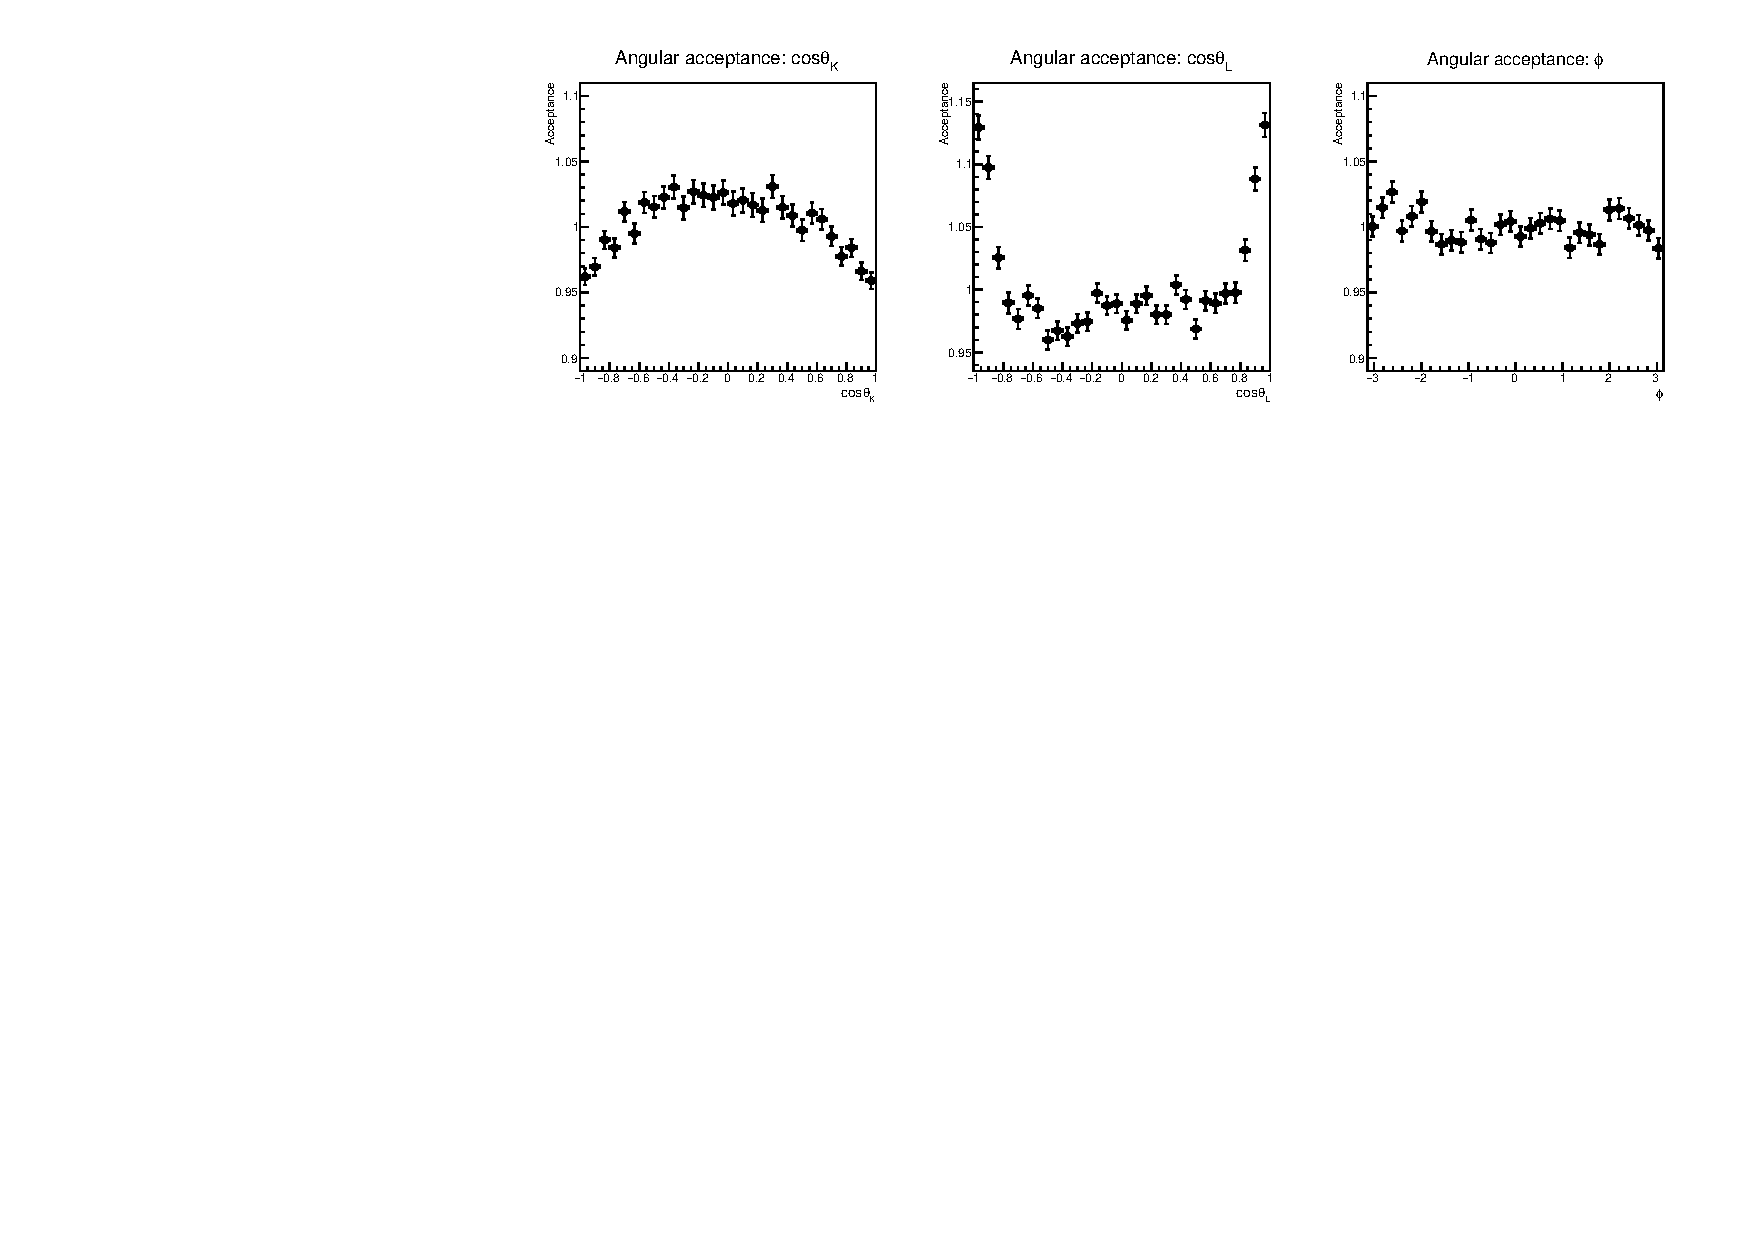
\includegraphics[width=1.05\linewidth]{AnglesAcc/AngAcc_MCfull_TupleBsDetached.pdf}\\
     \vspace*{-0.5cm}
  \end{center}
    \caption{
    The angular acceptance projections as function of the three helicity angles for full simulated $\Bs\to\jpsi(\epem)\phi$ sample.
}
  \label{fig:AnglesAccMCfull} 
\end{figure}

\begin{figure}[hbt]
  \begin{center}
    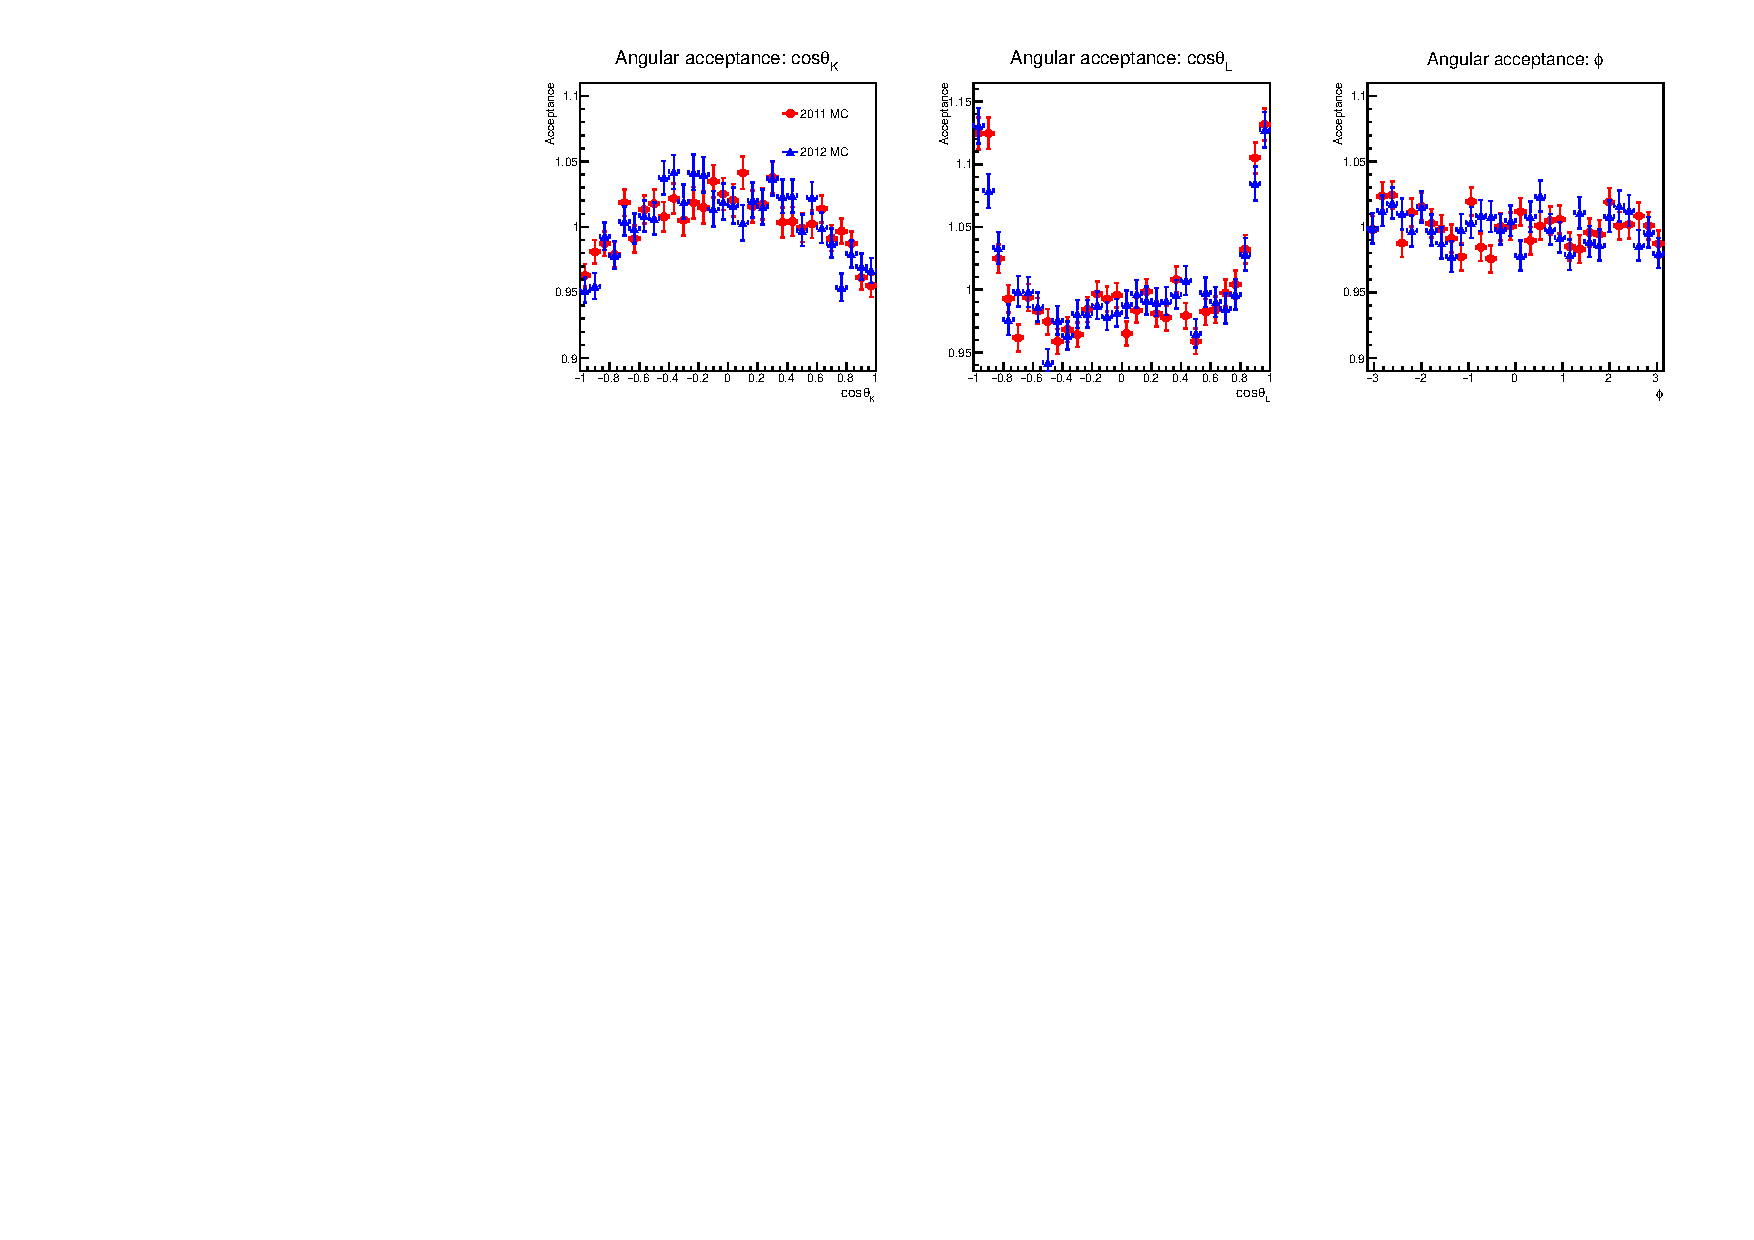
\includegraphics[width=1.05\linewidth]{AnglesAcc/AngAcc_MC11_MC12_TupleBsDetached.pdf}\\
     \vspace*{-0.5cm}
  \end{center}
    \caption{
    The angular acceptance projections as function of the three helicity angles for simulated $\Bs\to\jpsi(\epem)\phi$ events. 2011 and 2012 samples are compared.
}
\label{fig:AnglesAccMC11MC12} 
\end{figure}

\begin{figure}[hbt]
  \begin{center}
    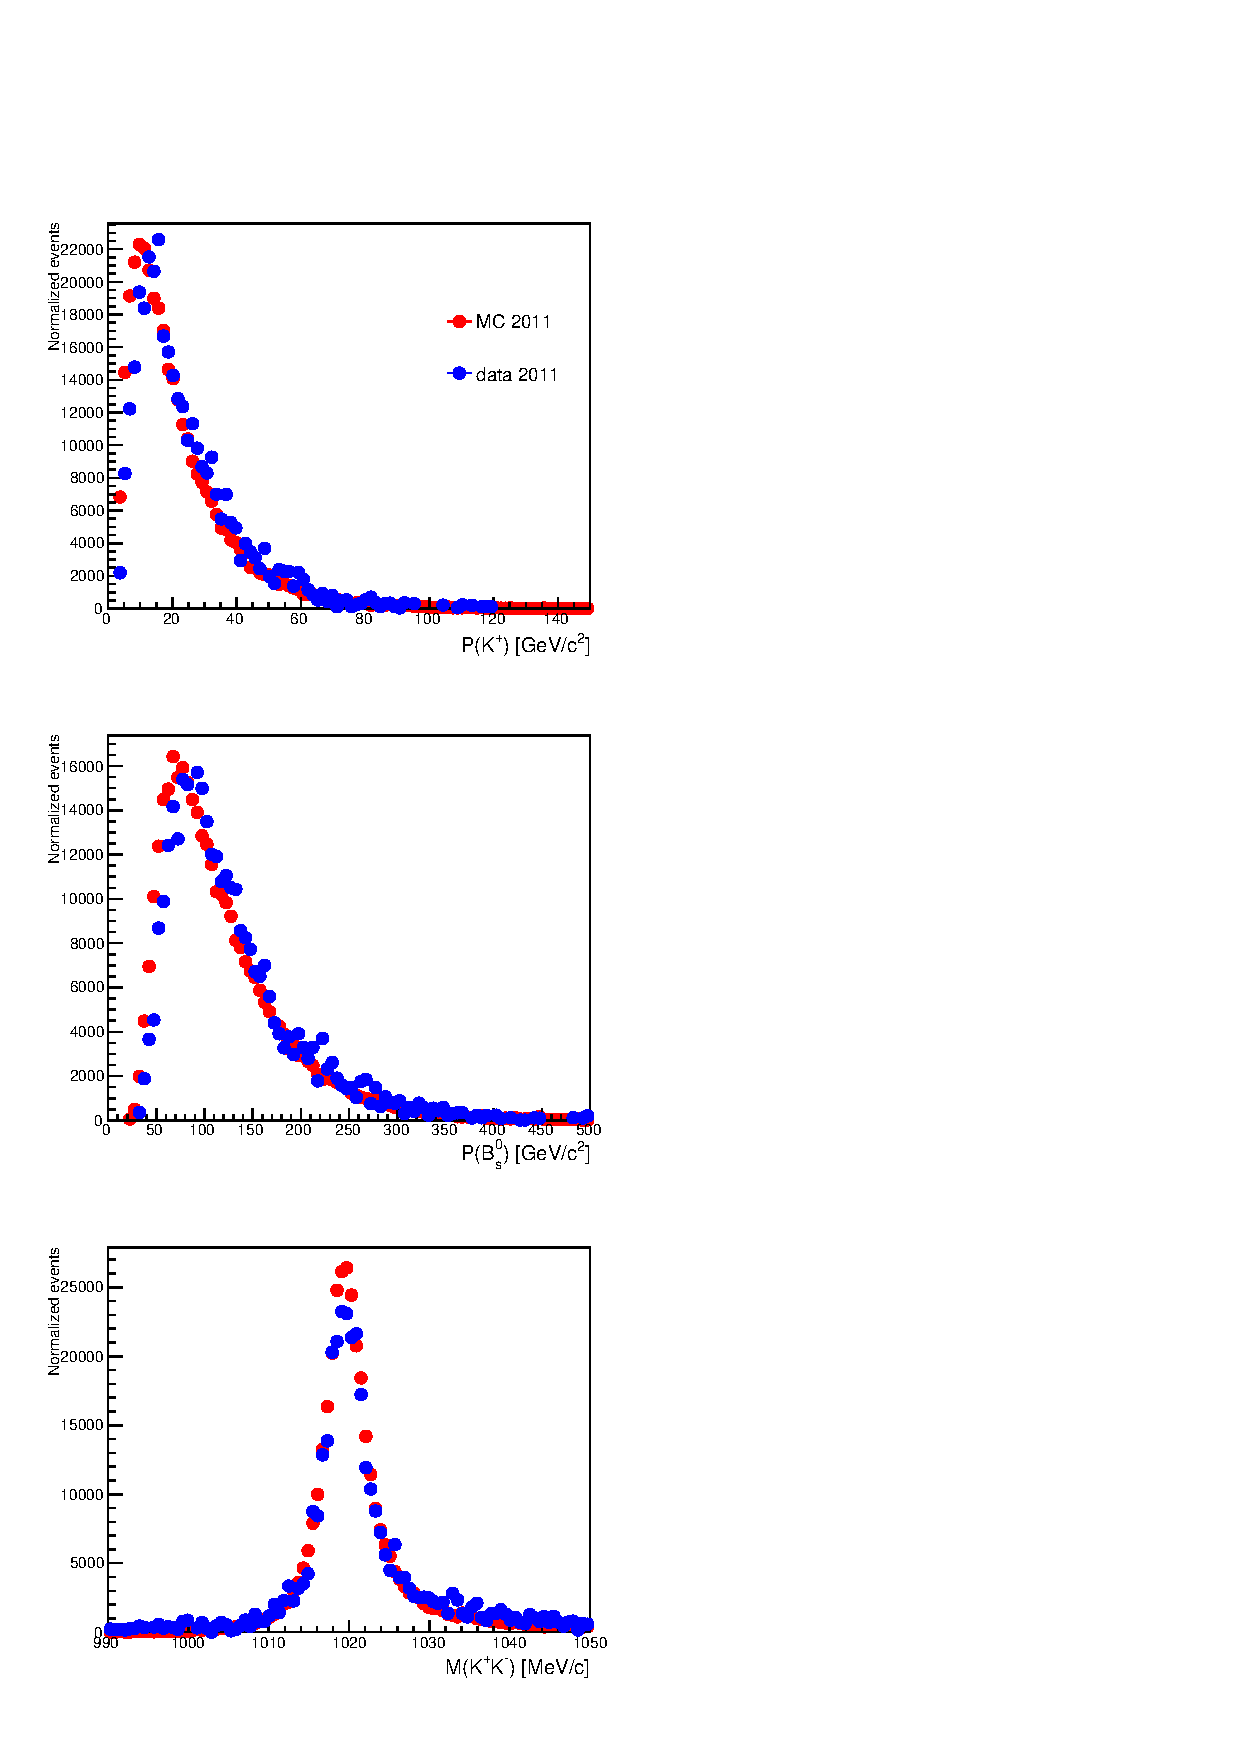
\includegraphics[width=0.48\linewidth]{AnglesAcc/AngAcc_IterMeth11.pdf}
    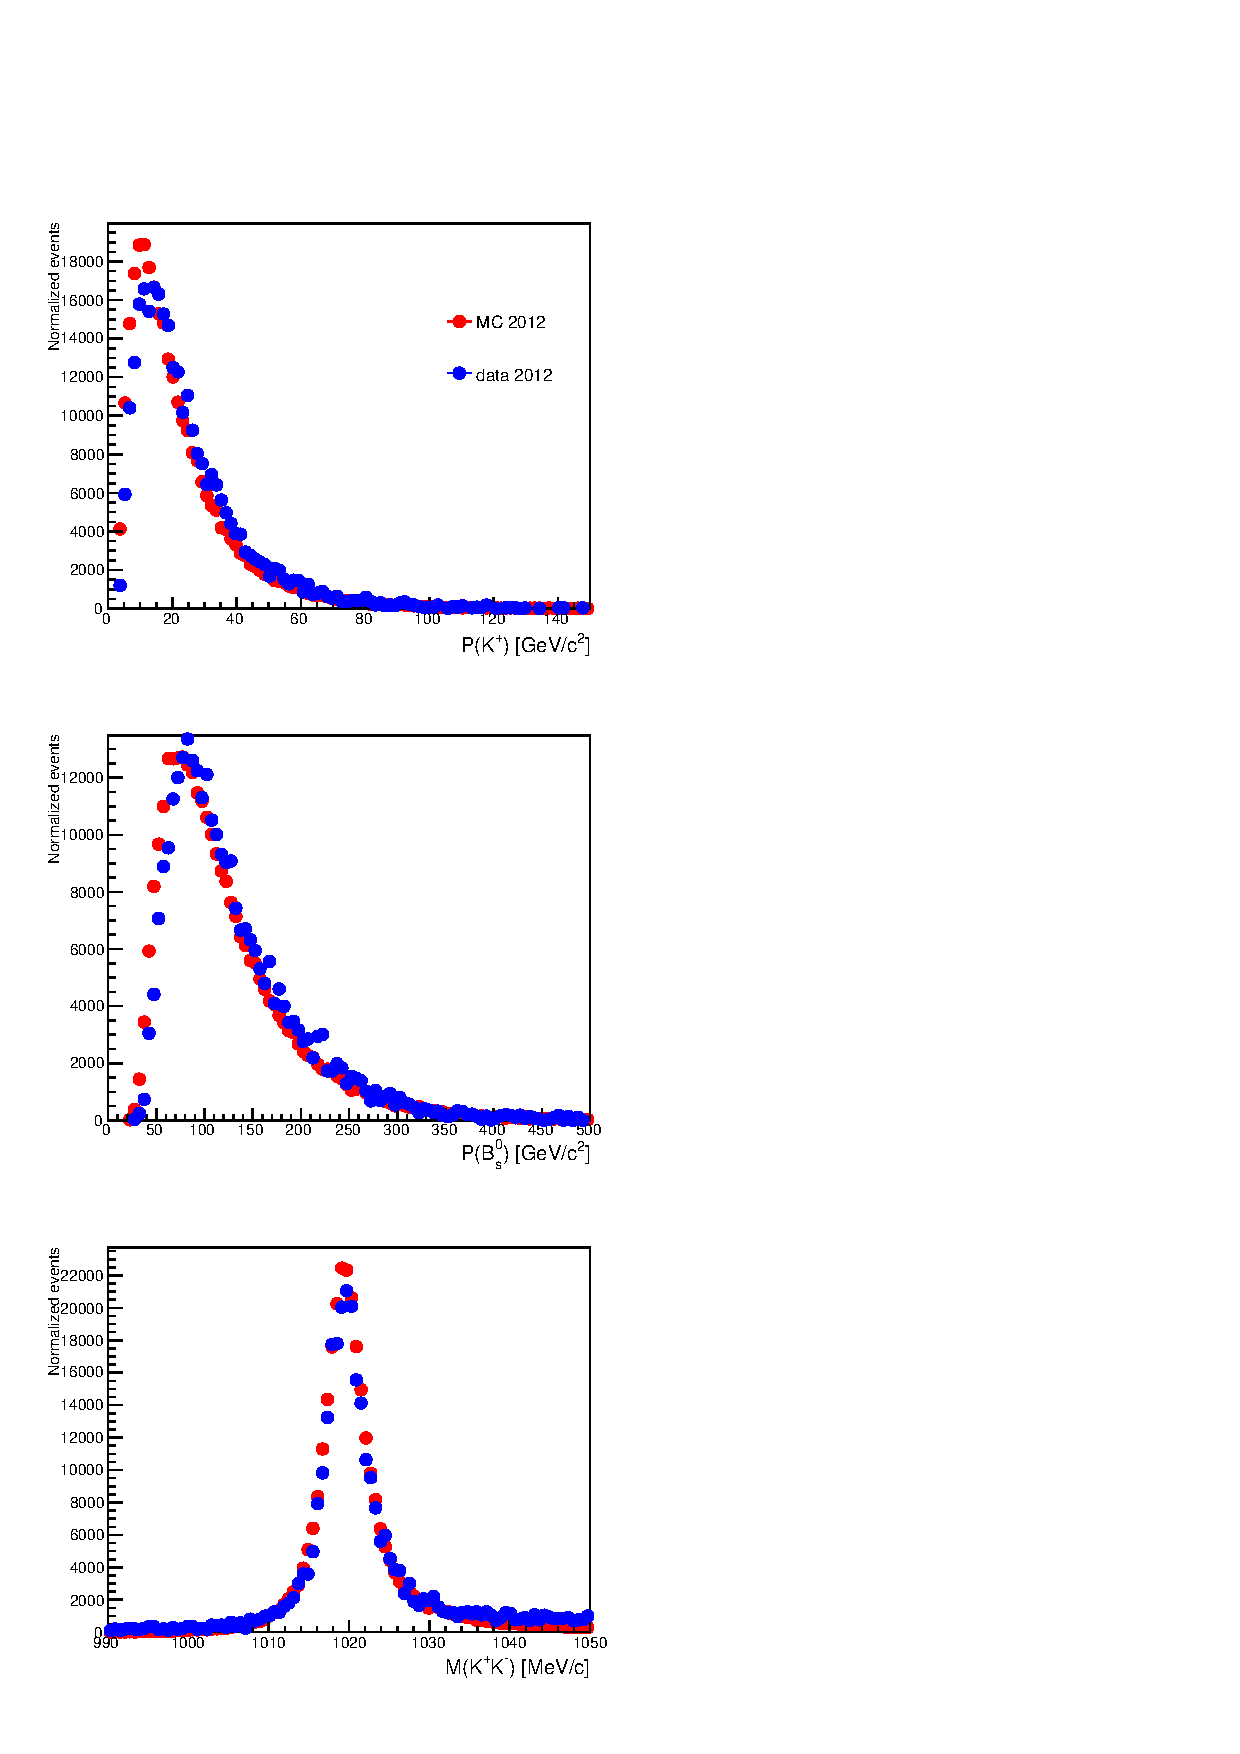
\includegraphics[width=0.48\linewidth]{AnglesAcc/AngAcc_IterMeth12.pdf}
     \vspace*{-0.5cm}
  \end{center}
    \caption{
    The comparison between the kinematical variables of $\Bs\to\jpsi(\epem)\phi$ signal events in sWeighted data (blue) and simulation data (red) for 2011 (left) and 2012 (right) run periods.
}
  \label{fig:AnglesAcc_IterMeth} 
\end{figure}
\clearpage

\section{Angular resolution}\label{sec:AngRes}

The angular resolution is defined as the difference between true and reconstructed angle in simulated sample. The one-dimensional projections of the three angular resolutions are shown in Fig.~\ref{fig:AnglesRes}. For angles $\theta_{K}$ and $\theta_{L}$, the used fitted model is a sum of three Gaussian functions, while for $\phi$ a double Gaussian plus a Voigtian component is required in order to better model the large non-Gaussian tails. The parameters determined from these fits are reported in Table~\ref{tab:AnglesRes}. It has been shown in Ref.~\cite{Aaij:2014-039} that there is no correlation between the resolution of the three angles. Two-dimensional distributions of the helicity angles are shown in Fig.~\ref{fig:AnglesRes2D}. 

Based upon studies performed in Ref.~\cite{Aaij:2014-039}, the effect from the angular resolution is negligible. It is considered as a source of systematic uncertainty in Sec.~\ref{subsec:Syst:AngRes}.

\begin{table}[htb]
  \caption{
    The fit results to the angular resolution distributions for each of the helicity angles taken from $\Bs\to\jpsi(\epem)\phi$ simulated signal sample for 2011 and 2012 run periods. The last row shows the effective Gaussian resolution computed for $\theta_{K}$ and $\theta_{L}$.
}
    \small{
 \begin{center}
  \begin{tabular}{cccc}
   \hline
    & 3 Gaussian & 3 Gaussian & 2 Gaussian+Voigtian\\
  \hline
  Parameter & $\theta_{L}$ &  $\theta_{K}$ &$\phi$\\
  \hline
    $\sigma_{1}$[mrad]  & 20.61$\pm$0.18 &  12.66$\pm$0.06 &  17.35$\pm$0.11 \\
    $\sigma_{2}$[mrad]  & 7.083$\pm$0.08 &  21.42$\pm$0.08 &  36.03$\pm$0.36 \\
    $\sigma_{3}$[mrad]  & 62.54$\pm$0.35 &  47.71$\pm$0.80 &  38.30$\pm$0.77 \\
    $\sigma_{4}$[mrad]  & - &  - &  83.00$\pm$1.20 \\
    $f_{1}$  & 0.3902$\pm$0.0026 &  0.3926$\pm$0.0058 &  0.4970$\pm$0.0073 \\
    $f_{2}$  & 0.1545$\pm$0.0031 &  0.5632$\pm$0.0052 &  0.4027$\pm$0.0056 \\
    $f_{3}$  & 0.4553$\pm$0.0040 &  0.0442$\pm$0.0078 &  0.1003$\pm$0.0091 \\
    \hline
    $\sigma_{eff}$[mrad]  & 44.21$\pm$0.34 &  20.54$\pm$0.45 &  - \\
   \hline
    \end{tabular}
  \end{center}
   }
\label{tab:AnglesRes}
\end{table}

\begin{figure}[hbt]
  \begin{center}
    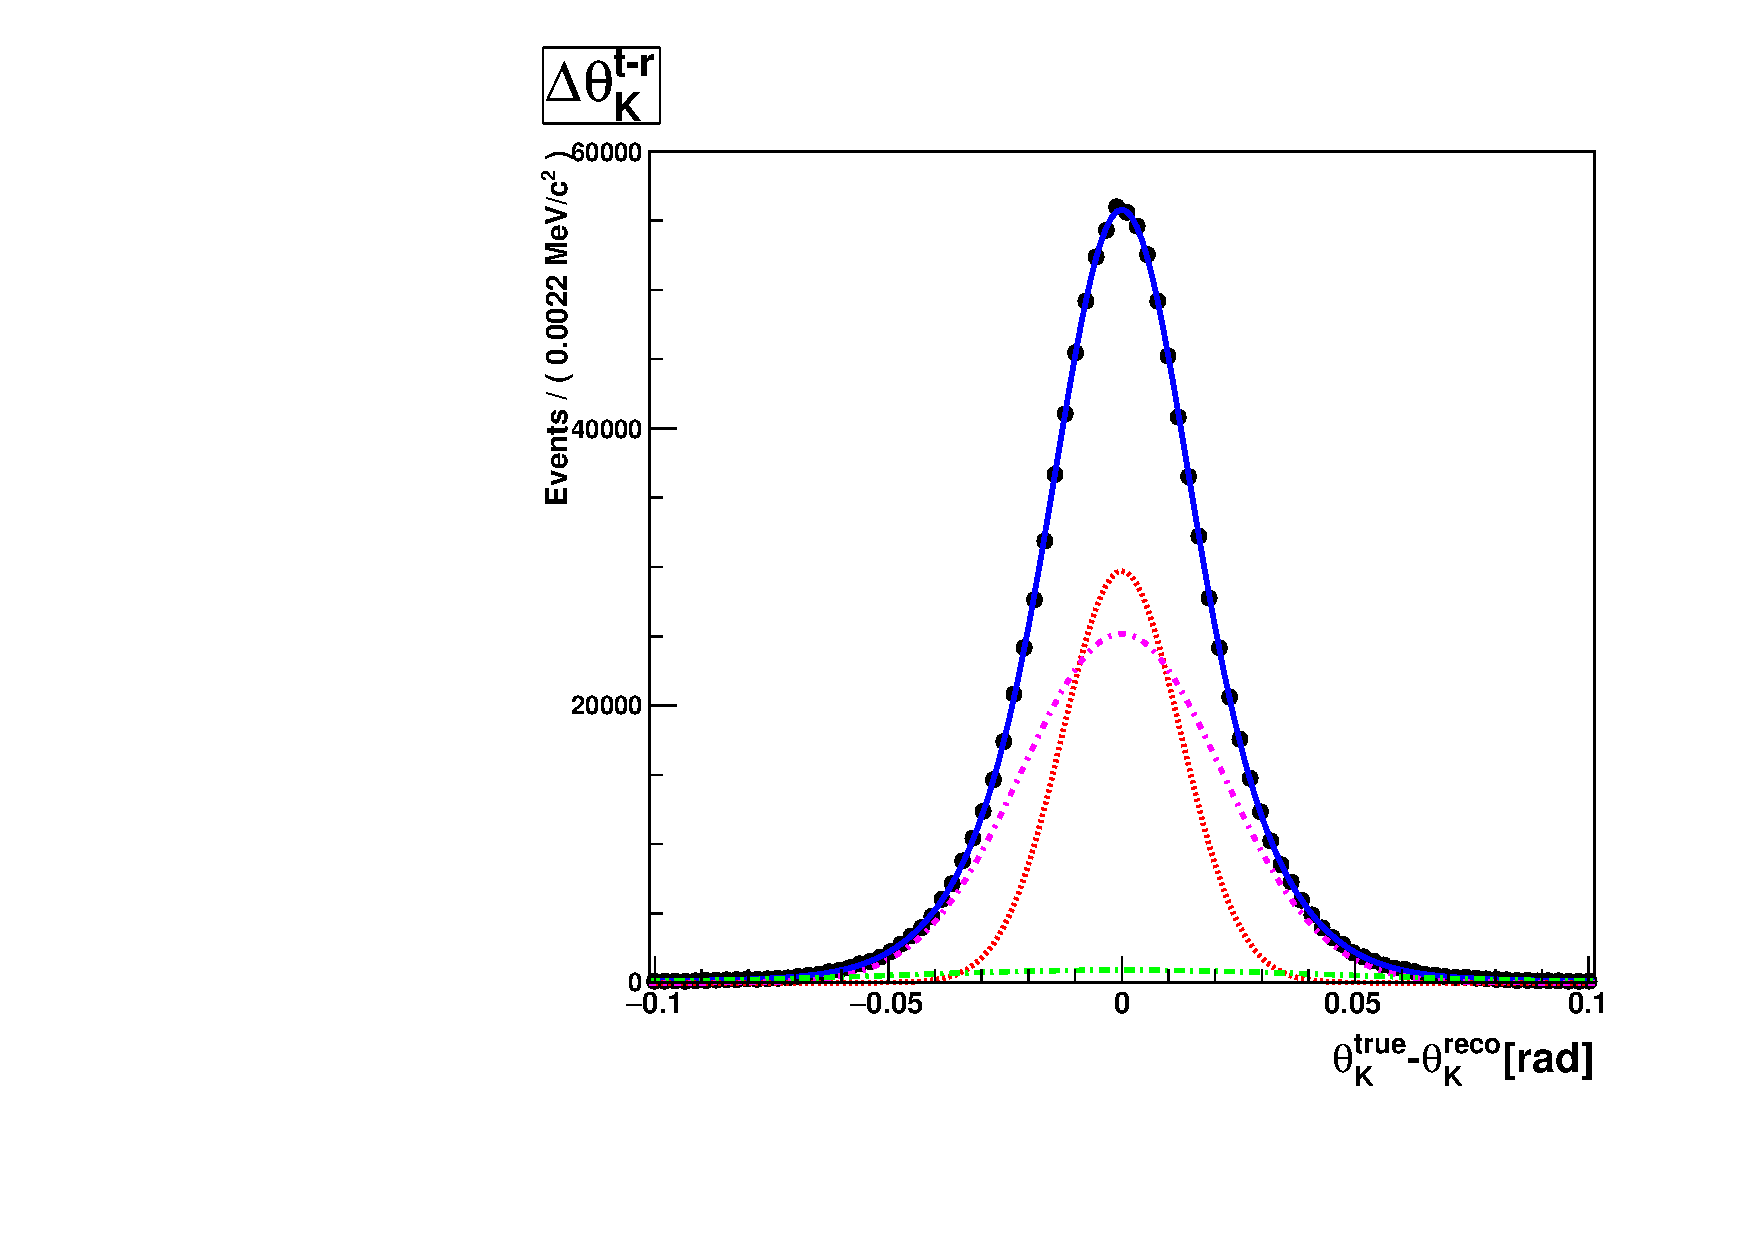
\includegraphics[width=0.47\linewidth]{AnglesRes/MC/thetaK_diff.pdf}
    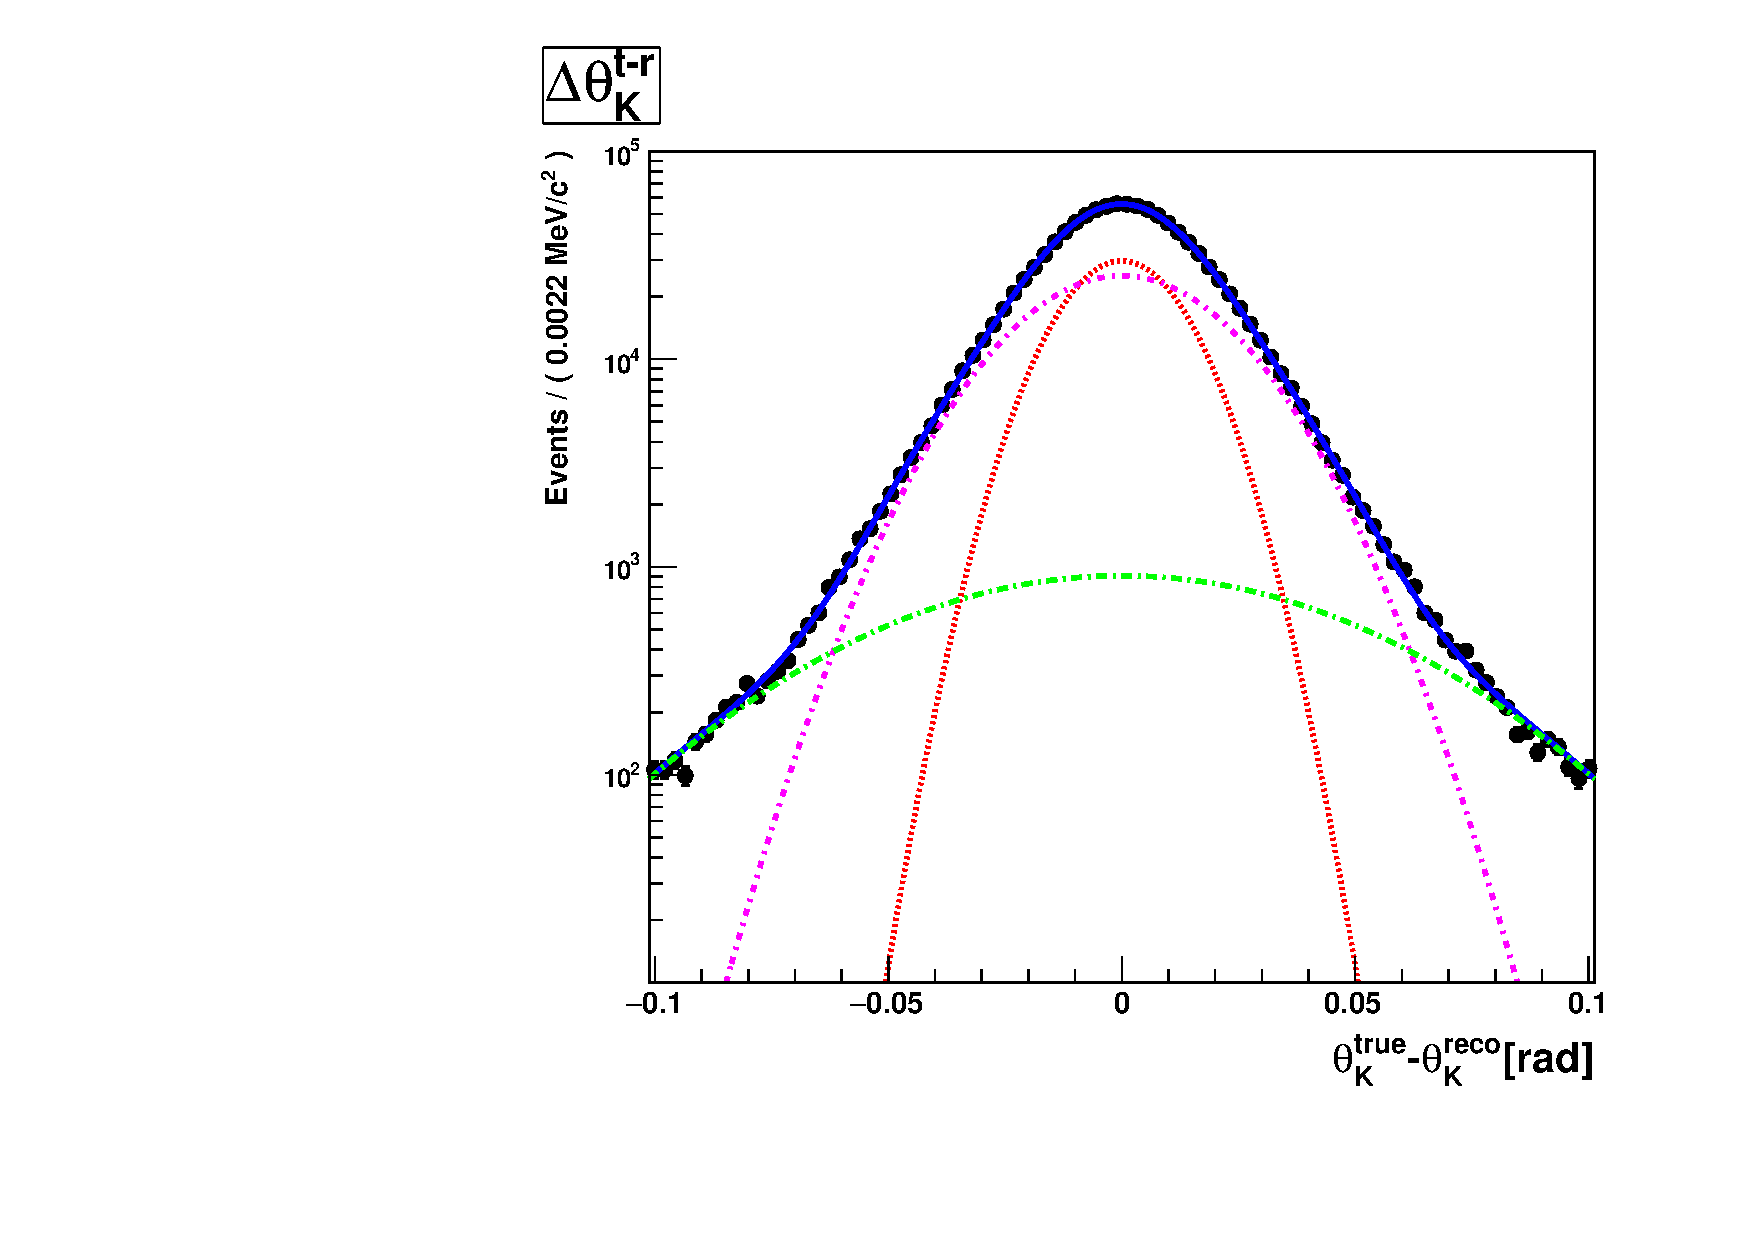
\includegraphics[width=0.47\linewidth]{AnglesRes/MC/thetaK_diff_log_new.pdf}
     \vspace*{-0.5cm}
  \end{center}
  \begin{center}
    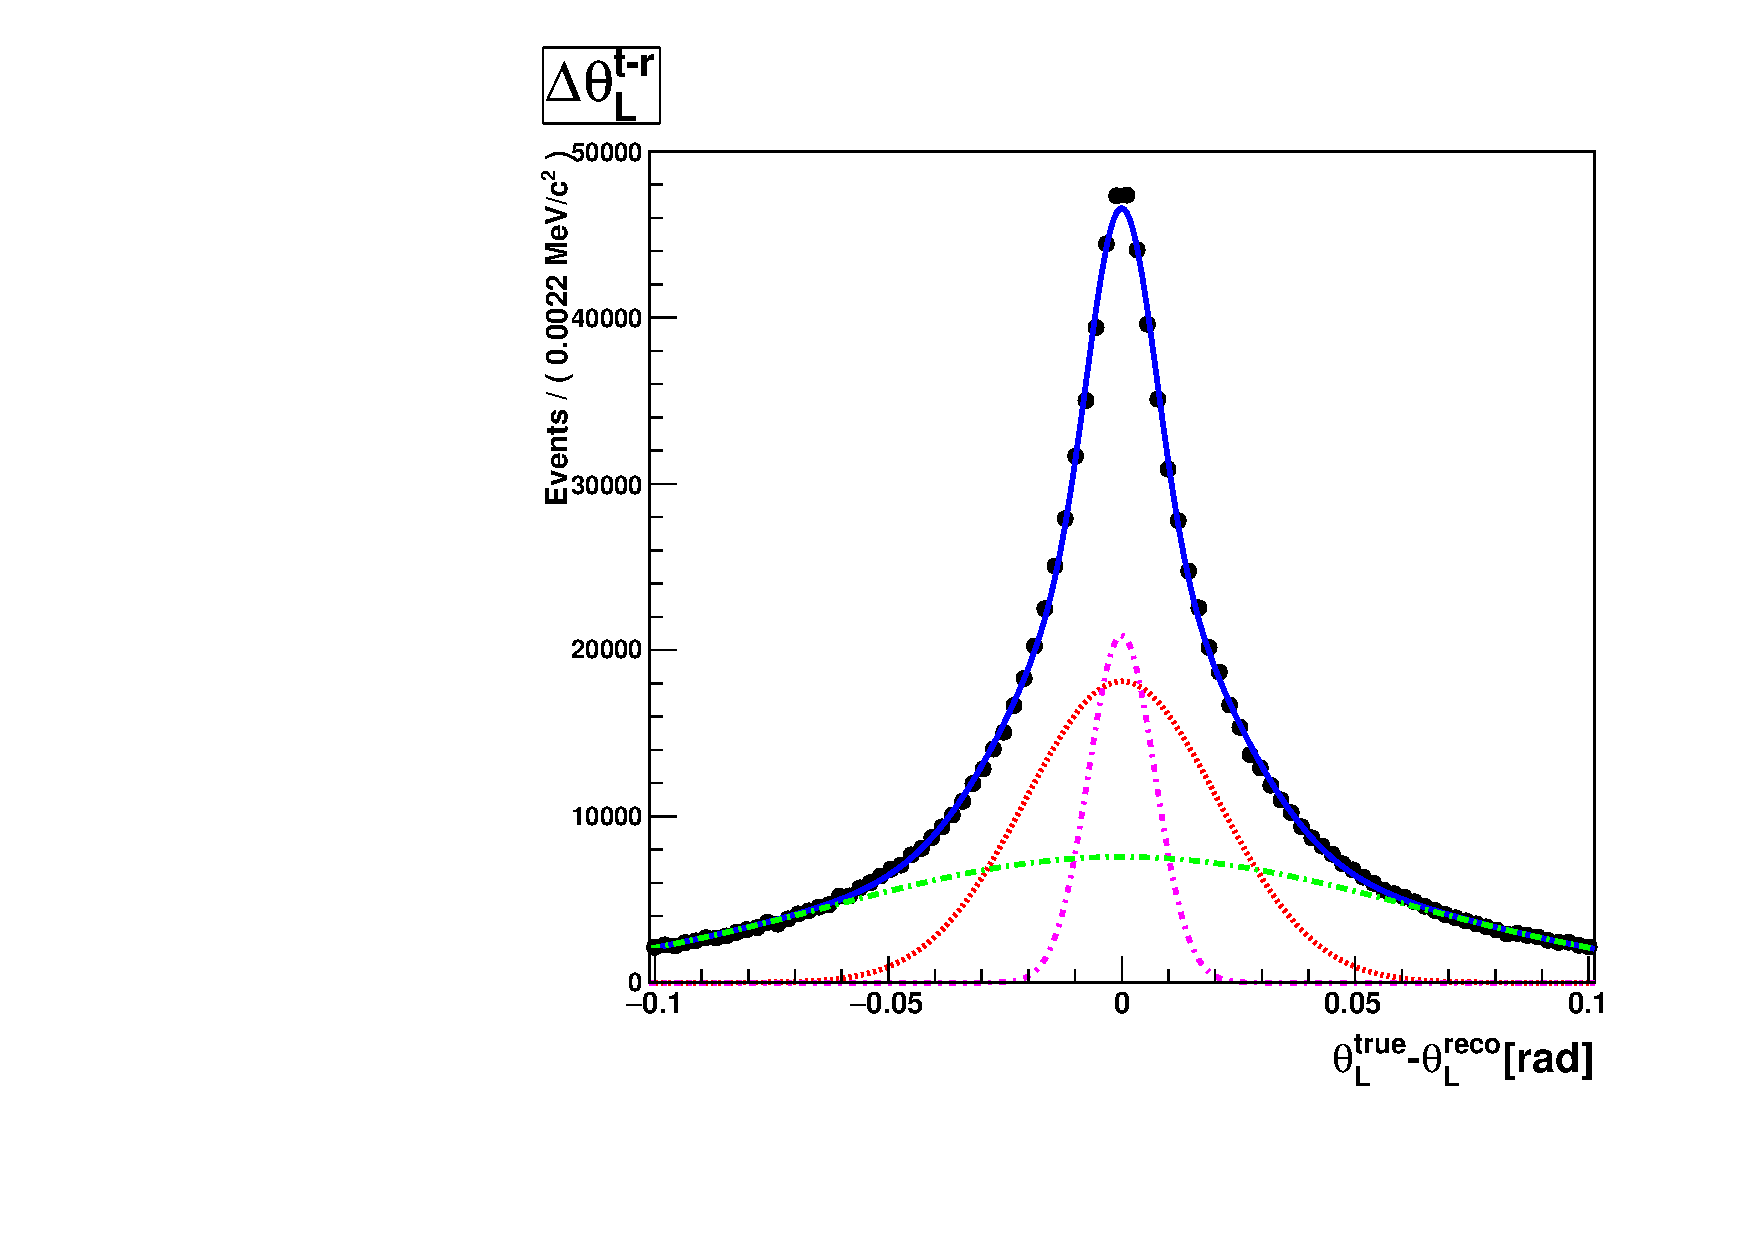
\includegraphics[width=0.47\linewidth]{AnglesRes/MC/thetaL_diff.pdf}
    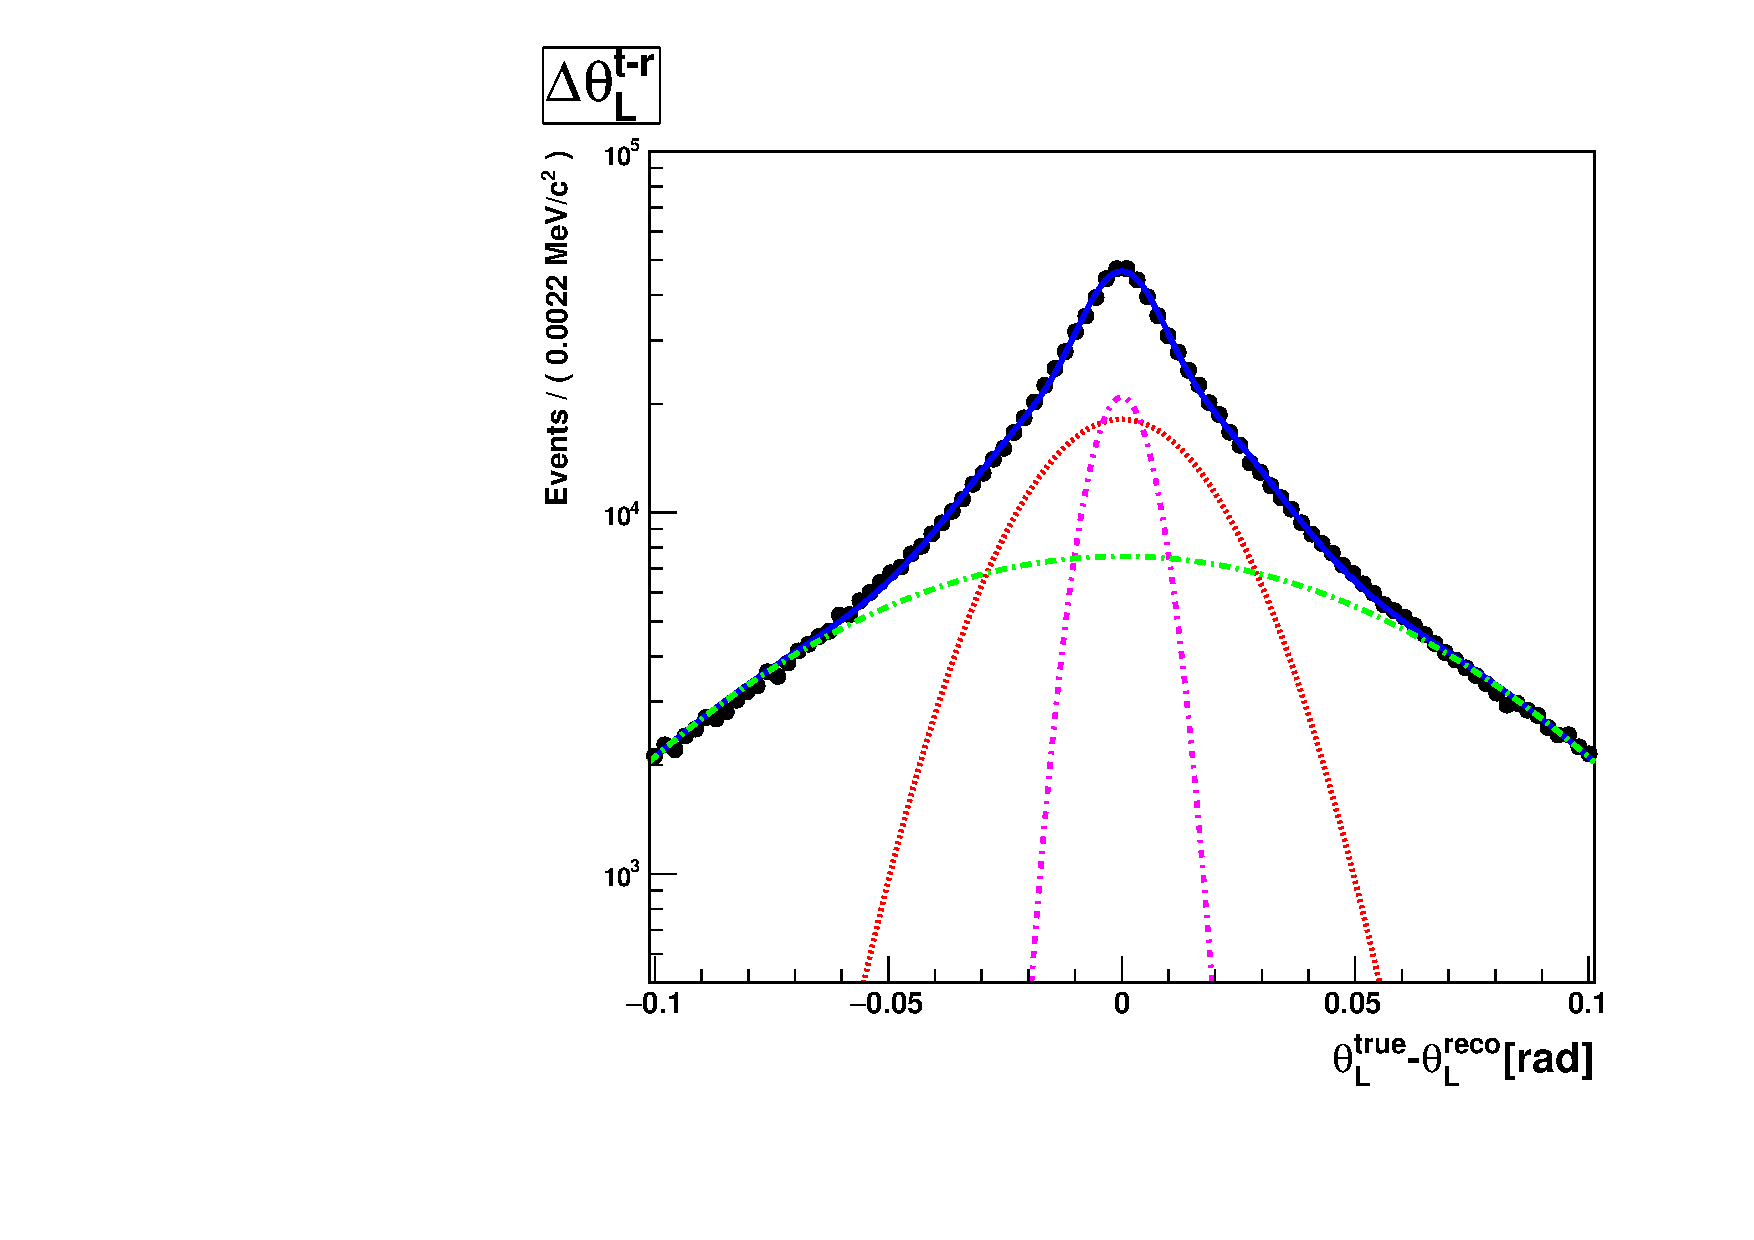
\includegraphics[width=0.47\linewidth]{AnglesRes/MC/thetaL_diff_log_new.pdf}
     \vspace*{-0.5cm}
  \end{center}
  \begin{center}
    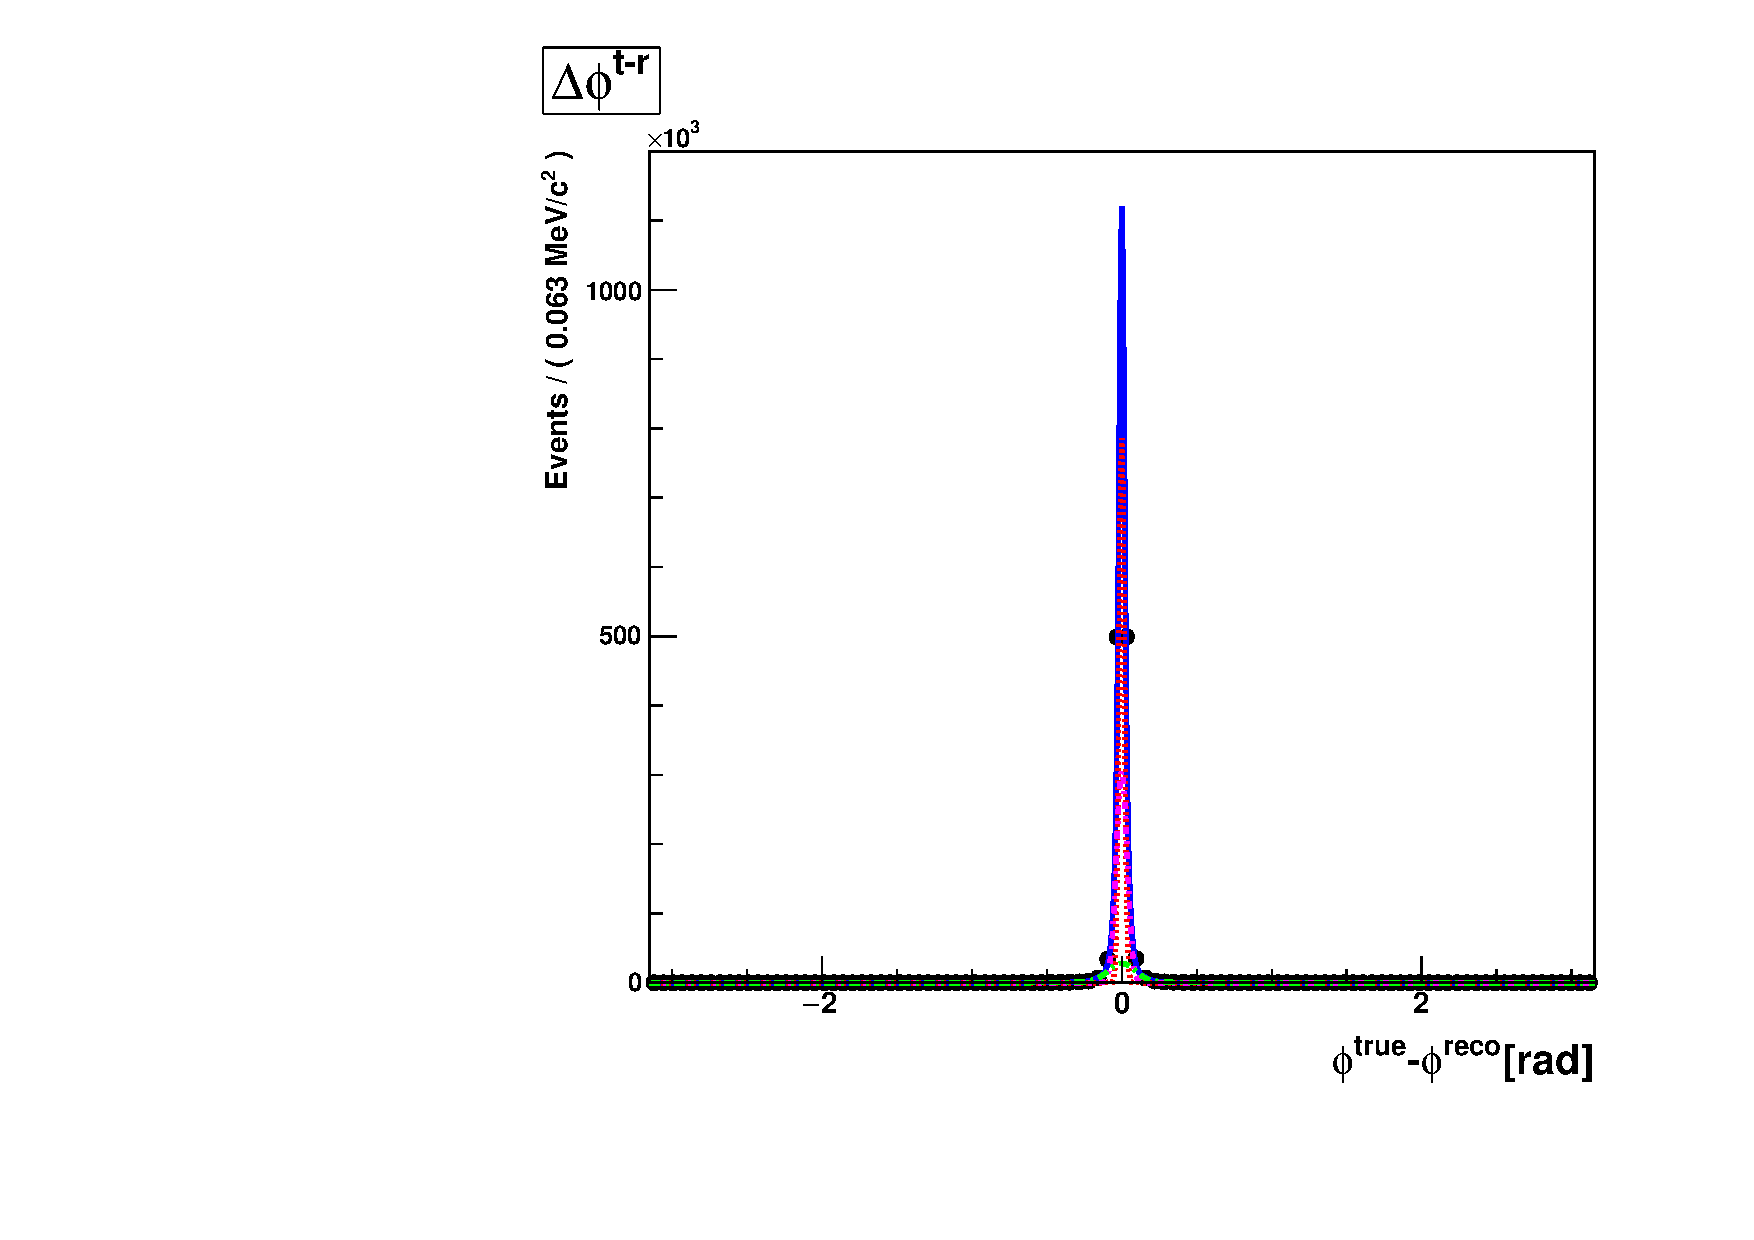
\includegraphics[width=0.47\linewidth]{AnglesRes/MC/phi_diff.pdf}
    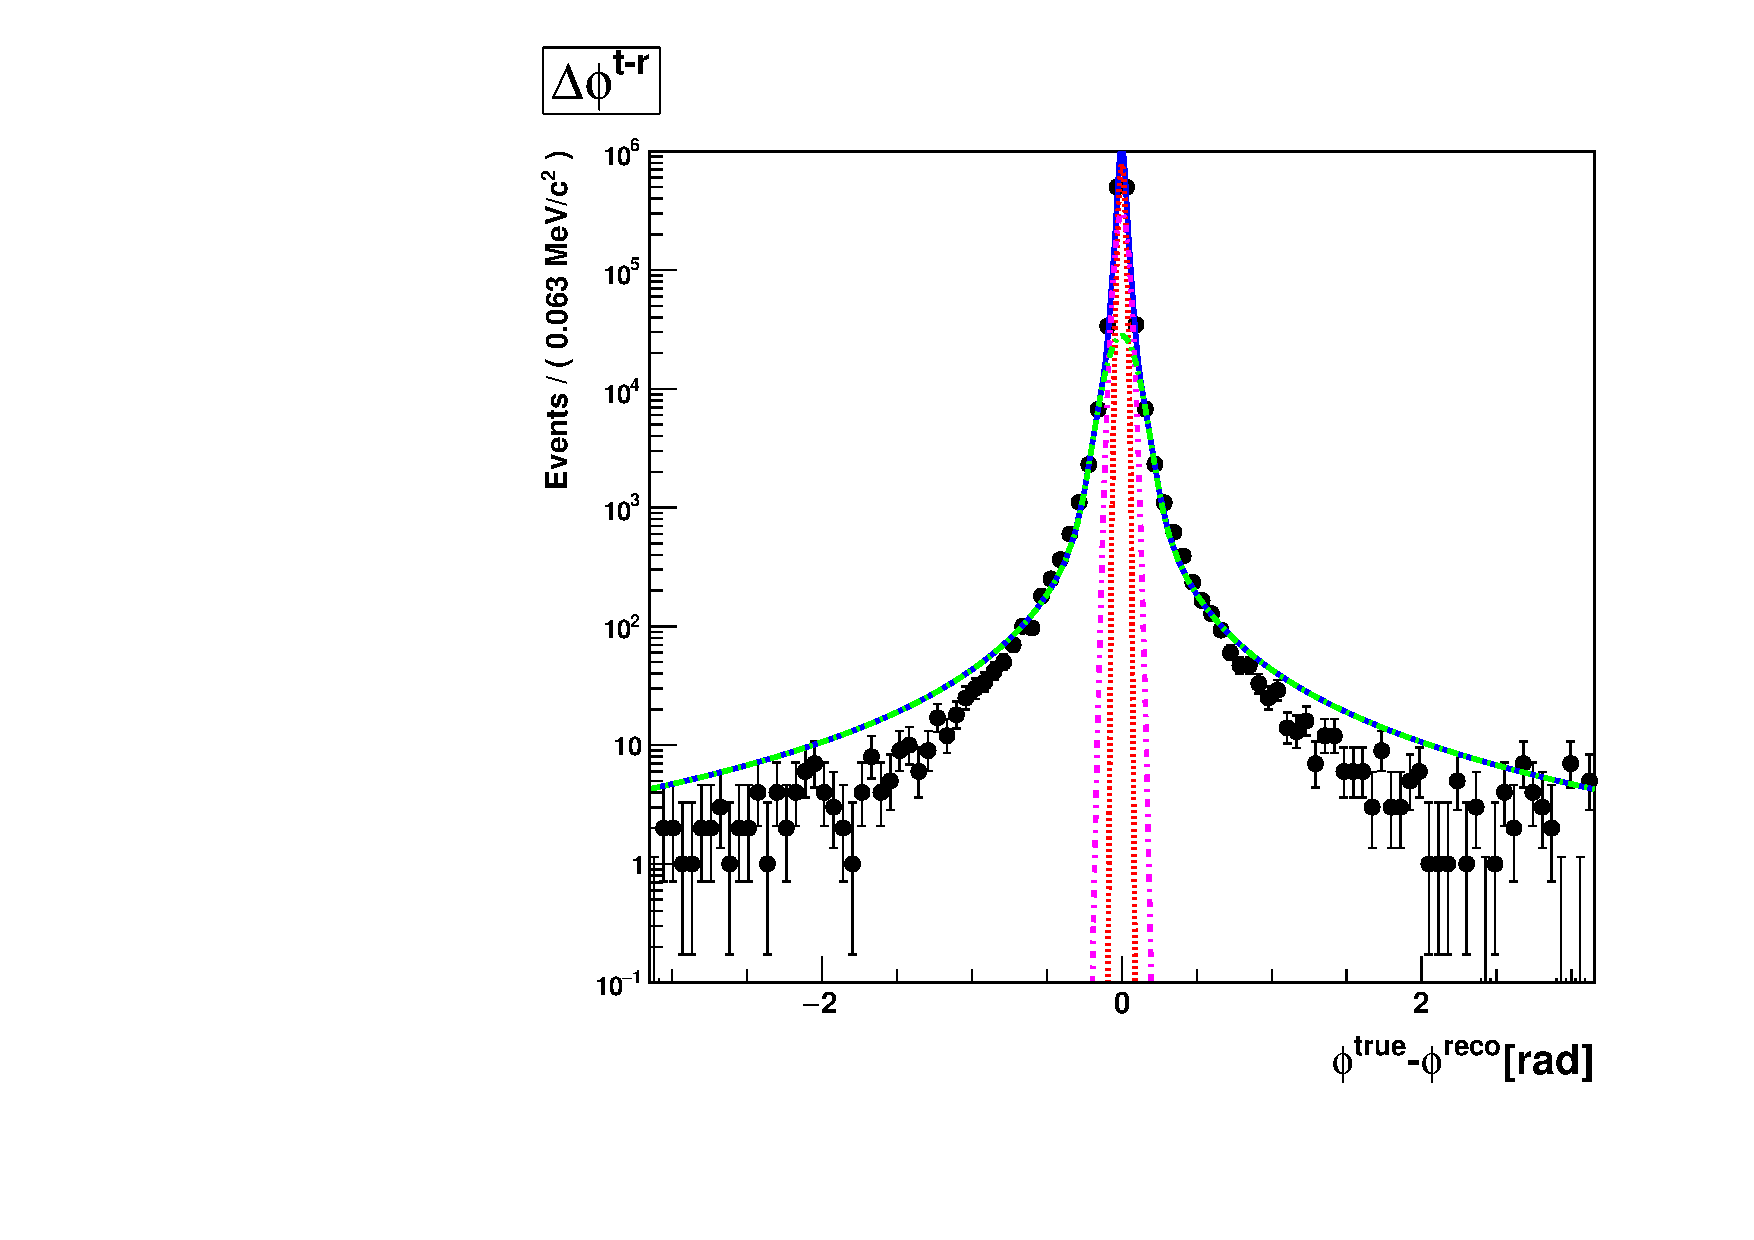
\includegraphics[width=0.47\linewidth]{AnglesRes/MC/phi_diff_log_new.pdf}
    \vspace*{-0.5cm}
  \end{center}
    \caption{
   The distributions of the difference between the true and reconstructed angle from the simulated sample of $\Bs\to\jpsi(\epem)\phi$ decays. A fit is superimposed in each distribution. The right hand side shows the logarithmic scale plots.
}
  \label{fig:AnglesRes} 
\end{figure}
\clearpage

\begin{figure}[hbt]
  \begin{center}
    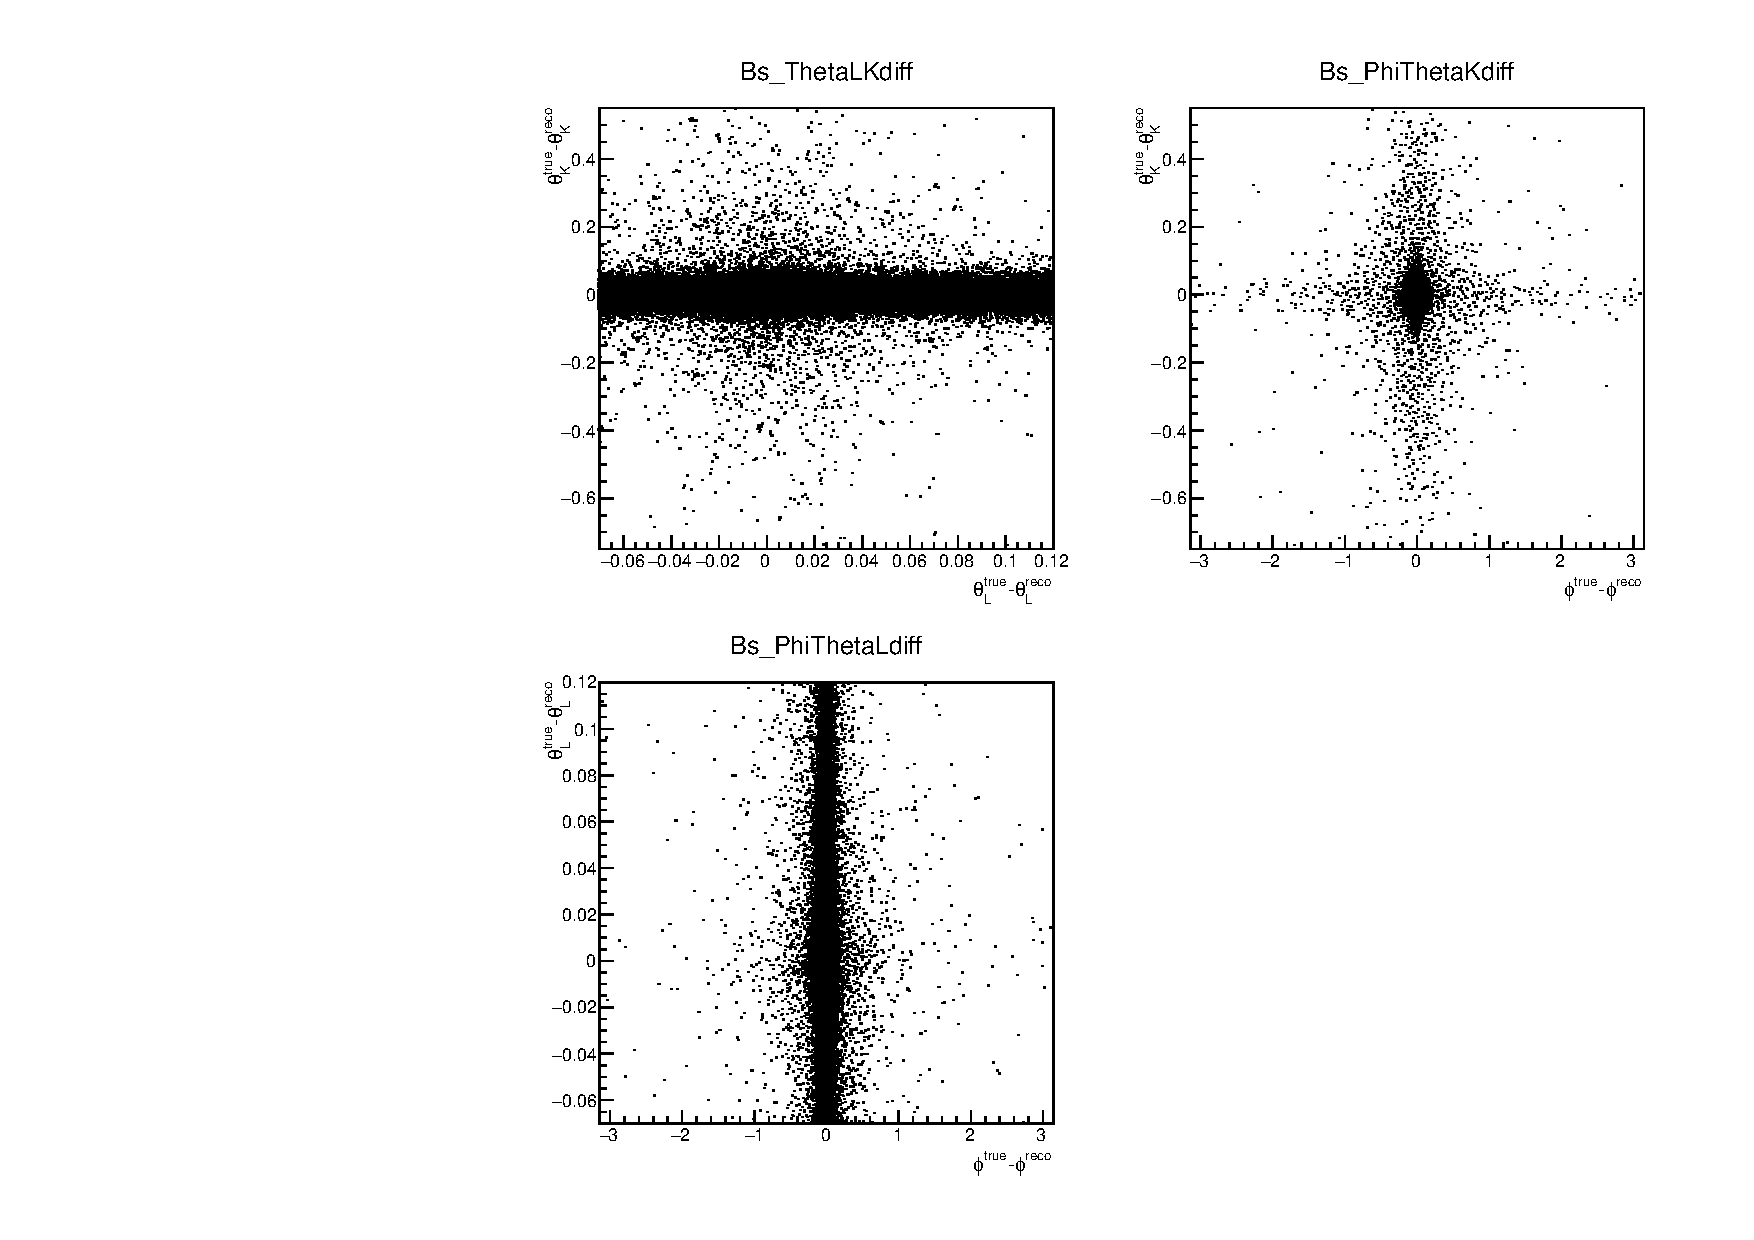
\includegraphics[width=0.9\linewidth]{AnglesRes/MC/AngRes_2D.pdf}
     \vspace*{-0.5cm}
  \end{center}
    \caption{
   The two-dimensional distributions of the helicity angle resolutions obtained from simulated data. The units are in radians in all cases.
}
  \label{fig:AnglesRes2D} 
\end{figure}
\clearpage

\section{Flavour tagging}\label{sec:FlavTagg}

The flavour of the $\Bs$ candidate at production state is inferred by two independent classes of flavour tagging algorithms, the opposite-side (OS) tagger and the same-side kaon (SSK) tagger, which exploit specific features of the incoherent production of $\bquark\bquarkbar$ quark pairs in $pp$ collisions. Each tagging algorithm gives a tag decision and a mistag probability. The tag decision takes three values: +1, -1, or 0, correspond to $\Bs$, $\Bsb$, or untagged $\Bs$ meson, respectively. The fraction of events in the sample with a non-zero tagging decision gives the efficiency of the tagger, $\varepsilon$. The mistag probability, $\eta$, is estimated event-by-event, and it represents the probability that the algorithm assigns a wrong tag decision to the event. It is calibrated using data samples of several flavour specific $\Bz$ and $\Bp$ decays, to obtain the corrected mistag probability, $\mistag$. The corrected mistag probability determines the square dilution factor of the tagger, $\langle\mathcal{D}^{2}\rangle=\langle(1-2\mistag)^{2}\rangle$. The $\langle\mathcal{D}^{2}\rangle$ rescales the efficiency of the tagger to quantify the fraction of the sample equivalent to perfectly tagged events. The effective efficiency, called tagging power, is given by the product of the efficiency and the square dilution factor, $\varepsilon\langle\mathcal{D}^{2}\rangle$.

By means of flavour conservation of the strong interaction, the OS tagger consists of a few algorithms~\cite{Aaij:2012mu}. They infer the signal production flavour from the decay products of the $\bquark$-hadron produced by the other $\bquark$ quark in the event, by using the charge of muons or electrons from second $\Bs$ in semileptonic decays, the net charge of the opposite-side displaced vertex, and the charge of the kaon from opposite-side $\bquark\to\cquark\to\squark$ transitions. All algorithms are combined to provide a single OS tagging response. The cut-based selection of the tagging candidates and the neural networks that calculate the mistag probabilities are optimized for the analysis of the full 2011 and 2012 datasets by using a data sample of $\Bp\to\jpsi\Kp$ decays. As an result, the OS algorithm has tagging power of (3.42$\pm$0.08)$\%$ in $\Bs\to\jpsi(\epem)\phi$ data, with a tagging efficiency of (36.31$\pm$0.45)$\%$. 

The SSK algorithm deduces the signal production flavour by exploiting charge-flavour correlations of the kaon produced during its fragmentation. A selection for the identification of the tagging kaon candidate is based on a neural network (NNetSSK)~\cite{LHCb:2012zja}. The NNetSSK algorithm~\cite{Aaij:2016psi} has a tagging efficiency of (62.83$\pm$0.45)$\%$ and a tagging power of (2.02$\pm$0.05)$\%$ in $\Bs\to\jpsi(\epem)\phi$ data.

The mistag probabilities, $\eta^{\text{alg}}$ (alg = OS, SSK), are calibrated on data to get the corrected probabilities $\mistag^{\text{alg}}$ and $\bar{\mistag}^{\text{alg}}$, for $\Bs$ and $\Bsb$, respectively:
\[
  \mistag^{\text{alg}}=\left(p_{0}^{\text{alg}}+\frac{\Delta p_{0}^{\text{alg}}}{2}\right)+\left(p_{1}^{\text{alg}}+\frac{\Delta p_{1}^{\text{alg}}}{2}\right)(\eta^{\text{alg}}-\langle\eta^{\text{alg}}\rangle)\quad\text{for an initial $\Bs$ event}, 
\]
\begin{equation}\label{eq:mistag}
 \bar{\mistag}^{\text{alg}}=\left(p_{0}^{\text{alg}}-\frac{\Delta p_{0}^{\text{alg}}}{2}\right)+\left(p_{1}^{\text{alg}}-\frac{\Delta p_{1}^{\text{alg}}}{2}\right)(\eta^{\text{alg}}-\langle\eta^{\text{alg}}\rangle)\quad\text{for an initial $\Bsb$ event},
\end{equation}
where $p^{\text{alg}}_{i}$ ($i$ = 0, 1) are the calibration parameters, averaged for $\Bs$ and $\Bsb$ events; $\Delta p^{\text{alg}}_{i}$, called mistag asymmetries, are the difference between the calibration parameters as measured for $\Bs$ and $\Bsb$. The $\langle\eta^{\text{ang}}\rangle$ is the average of the mistag distribution of the $\Bs\to\jpsi(\epem)\phi$ data, unfolded from background with the sPlot technique~\cite{Pivk:2004ty} by using the $\jpsi\phi$ mass as discriminating variable (Fig.~\ref{fig:Mistag}). The parameters used in Eq.~\ref{eq:mistag} are reported in Table~\ref{tab:CalibrationFT}. 
\begin{figure}[hbt]
  \begin{center}
    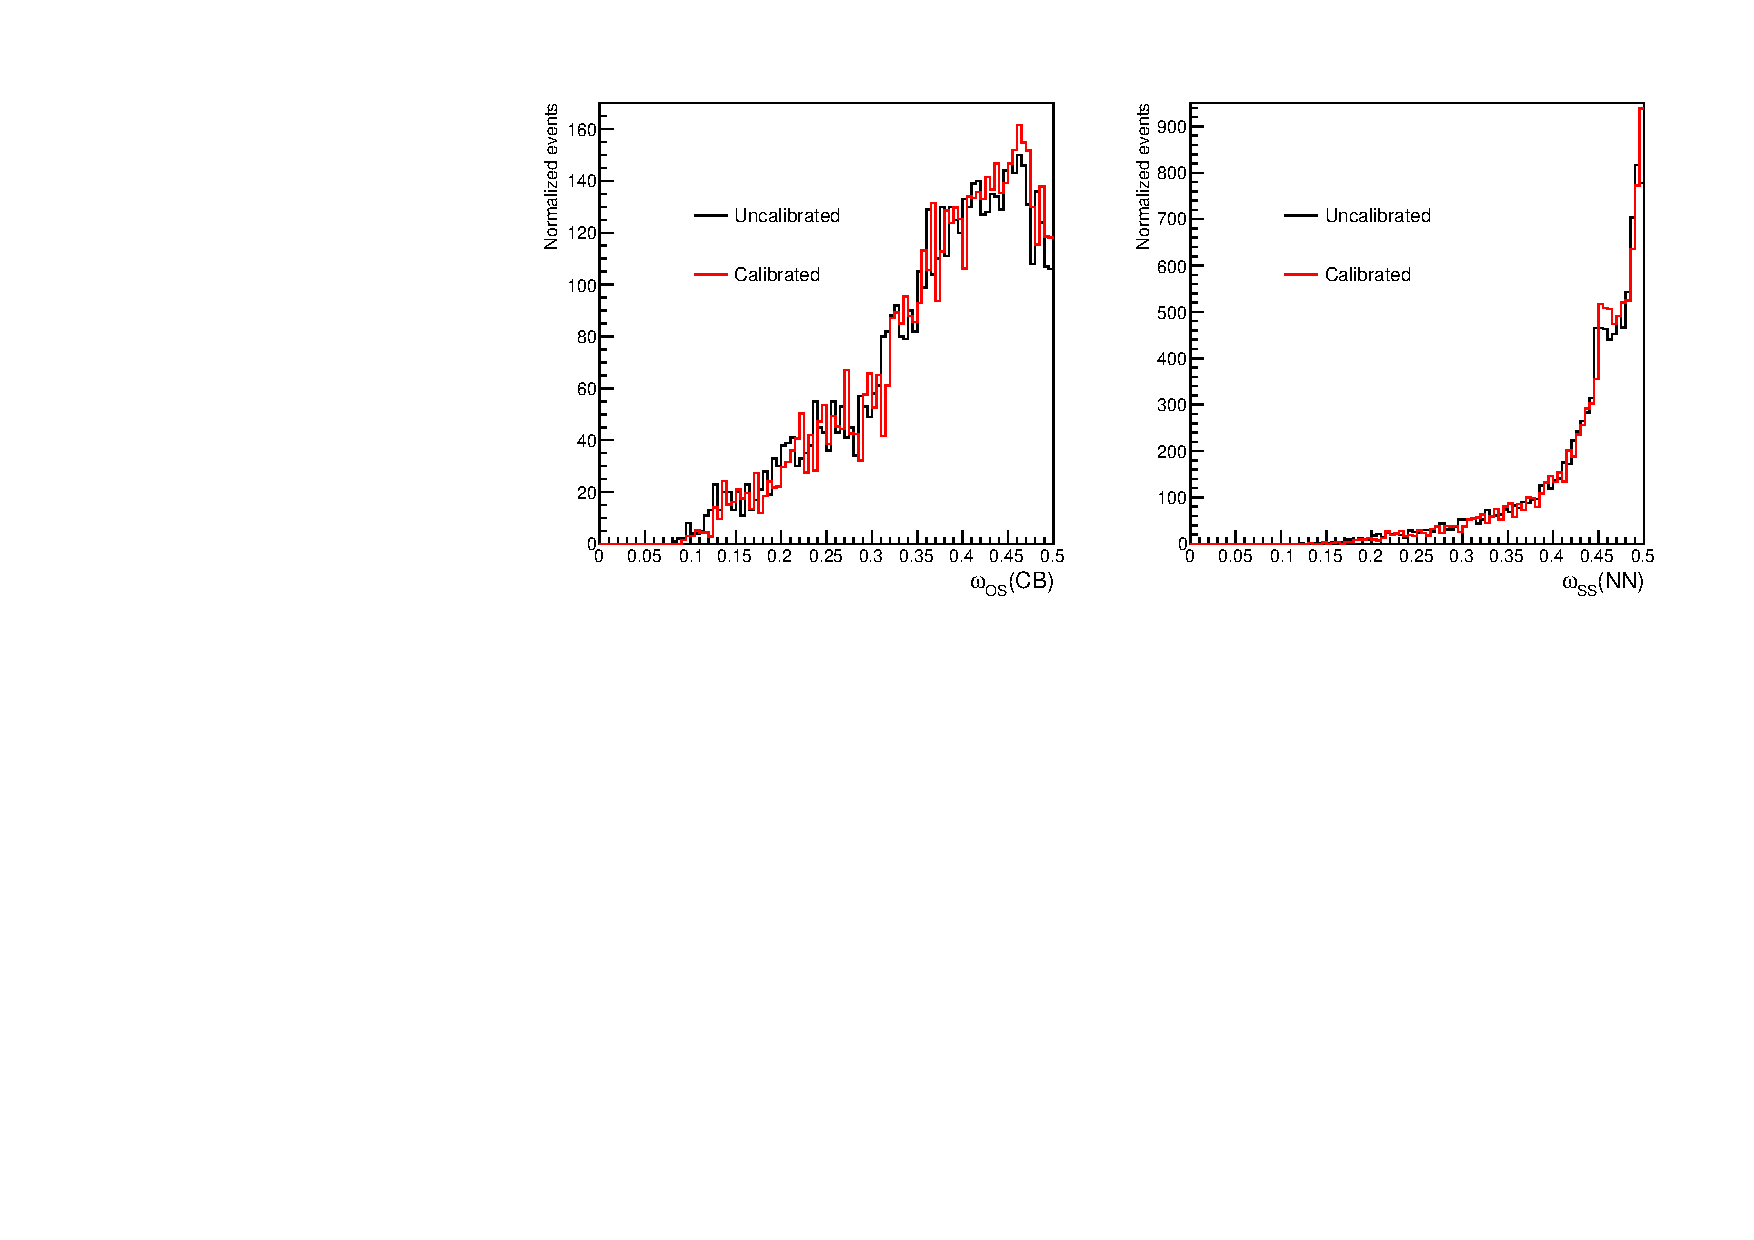
\includegraphics[width=1\linewidth]{Tagging/omega_OS_SS_fullRun1_horizontal.pdf}
     \vspace*{-0.5cm}
  \end{center}
    \caption{
   The OS (left) and SSK (right) mistag distributions for $\Bs\to\jpsi(\epem)\phi$ signal events before (black) and after (red) the calibration.}
  \label{fig:Mistag} 
\end{figure}
They are the results of the standard calibration provided by the Flavour Tagging group~\cite{LHCb:FTa, LHCb:FTb}: $p^{\text{OS}}_{i}$ are the combinations of calibration in data samples of several decays ($\Bu\to\jpsi\Kp$, $\Bu\to\Dz\pip$, $\Bz\to\jpsi\Kstarz$, $\Bz\to\Dstarm\mup X$ and $\Bs\to\Dsm\pip$); the OS mistag asymmetries are measured with $\Bu\to\jpsi\Kp$, $\Bu\to\Dz\pip$ and $\Bz\to\jpsi\Kstarz$ decays; $p^{\text{SSK}}_{i}$ are extracted by measuring the $\Bs$ flavour oscillations in a sample of $\Bs\to\Dsm\pip$ decays; the SSK mistag asymmetries are determined from a sample of prompt $\Dsp\to\phi\pip$ decays, reweighted to match the $\Bs$ kinematic distributions. Systematic uncertainties of calibration parameters address the portability of the calibrations from the control samples to $\Bs\to\jpsi(\epem)\phi$ data; they are dominated by the effect of the different kinematic distributions between the decay modes used in calibration and the $\Bs\to\jpsi(\epem)\phi$ signal data. Such systematic errors are independent from the flavour decision, and they mainly cancel when computing the mistag asymmetries. Their small contribution - approximately 10$\%$ (20$\%$) of the systematic error of $p_{0}$ ($p_{1}$) for $\Delta p_{0}/2$ ($\Delta p_{1}/2$) - are directly included in the single errors of the mistag asymmetries reported in Table~\ref{tab:CalibrationFT}.

 \begin{table}[htb]
  \caption{
   The parameters used in Eq.~\ref{eq:mistag} to calibrate the per-event mistag probabilities. When two uncertainties are quoted, the first one is statistical and the second one is systematic.}
    \small{
\begin{center}\begin{tabular}{ccc}
    Parameter                         &  OS  & SSK  \\ 
    \hline
   $\langle\eta\rangle$& 0.3751&   0.4373 \\
    $p_{0}-\langle\eta\rangle$ &   0.0062$\pm$0.0019$\pm$0.0040 & 0.005$\pm$0.004$\pm$0.003 \\
    $\Delta p_{0}/2$& 0.0070$\pm$0.0006 &    -0.0079$\pm$0.0007 \\
    $p_{1}$ &   0.982$\pm$0.007$\pm$0.034 & 0.976$\pm$0.071$\pm$0.057 \\
    $\Delta p_{1}/2$& 0.033$\pm$0.006 &    0.0035$\pm$0.0111 \\
    \hline
  \end{tabular}\end{center}
  }
\label{tab:CalibrationFT}
\end{table}

The $\Bs\to\jpsi(\epem)\phi$ data sample is split in four independent subsamples, according to the tag decisions: exclusive OS tagged events ($q^{\text{OS}}\neq$0 and $q^{\text{SSK}}$=0), referred to as "OS-only" events; exclusive SSK tagged events ($q^{\text{OS}}$=0 and $q^{\text{SSK}}\neq$0), referred to as "SSK-only" events; OS and SSK tagged events ($q^{\text{OS}}\neq$0 and $q^{\text{SSK}}\neq$0), referred to as "OS$\&$SSK" events; and finally, untagged events ($q^{\text{OS}}$=$q^{\text{SSK}}$=0), which are about 22$\%$ and 26$\%$ of the data and simulation samples, respectively. The fractions, the efficiencies, and the tagging powers of the tagged categories OS-only, SSK-only and OS$\&$SSK as measured for $\Bs\to\jpsi(\epem)\phi$ signal candidates from full 2011 and 2012 datasets and from full simulation sample are reported in Tables~\ref{tab:FTperformanceRDfull} and~\ref{tab:FTperformanceMCfull}, respectively. The total tagging efficiency and tagging power of data sample are (75.70$\pm$0.68)$\%$ and (5.20$\pm$0.10)$\%$, respectively. In case of simulated data, the total tagging efficiency and tagging power are (74.73$\pm$0.13)$\%$ and (5.38$\pm$0.02)$\%$, respectively. The flavour tagging performance obtained using simulation is in agreement with flavour tagging performance for data within statistical uncertainty.

\begin{table}[htb]
  \caption{
   The summary of the tagging efficiency ($\varepsilon$), square dilution factor ($\mathcal{D}^{2}$) and tagging power ($\varepsilon\mathcal{D}^{2}$) for the different categories of tagger, obtained from $\Bs\to\jpsi(\epem)\phi$ {\bf signal candidates from full 2011 and 2012 data samples} after the tagging calibration. The column "Fraction" reports the fraction of events in each category out of the all tagged events. }
    \small{
\begin{center}\begin{tabular}{ccccc}
   \hline
    Category & Fraction($\%$)&$\varepsilon(\%)$ & $\mathcal{D}^{2}$ & $\varepsilon\mathcal{D}^{2}(\%)$\\
  \hline
    OS-only& 17.0 &12.87$\pm$0.31 &  0.0977$\pm$0.0025  &1.26$\pm$0.05 \\
     SSK-only& 52.0 &39.39$\pm$0.46 & 0.0315$\pm$0.0013 & 1.24$\pm$0.04 \\
     OS$\&$SSK& 31.0 &23.44$\pm$0.40 &  0.1152$\pm$0.0020  &2.70$\pm$0.08 \\
    \hline
     Total& 100 &75.70$\pm$0.68 & 0.0687$\pm$0.0033 & 5.20$\pm$0.10 \\
    \hline
    \end{tabular}\end{center}
  }
\label{tab:FTperformanceRDfull}
\end{table}
\begin{table}[htb]
  \caption{
   The summary of the tagging efficiency ($\varepsilon$), square dilution factor ($\mathcal{D}^{2}$) and tagging power ($\varepsilon\mathcal{D}^{2}$) for the different ctegories of tagger, obtained from $\Bs\to\jpsi(\epem)\phi$ {\bf signal candidates from full simulated data sample} after the tagging calibration has been applied. The column "Fraction" reports the fraction of events in each category out of the all tagged events. }
    \small{
\begin{center}\begin{tabular}{ccccc}
   \hline
    Category & Fraction($\%$)&$\varepsilon(\%)$ & $\mathcal{D}^{2}$ & $\varepsilon\mathcal{D}^{2}(\%)$\\
  \hline
    OS-only& 16.7 &12.46$\pm$0.06 &  0.0995$\pm$0.0006 &  1.24$\pm$0.01 \\
     SSK-only& 54.0&40.33$\pm$0.09 &  0.0347$\pm$0.0003 &  1.40$\pm$0.01 \\
     OS$\&$SSK& 29.3&21.94$\pm$0.07 &  0.1249$\pm$0.0005 &  2.74$\pm$0.02 \\
    \hline
     Total& 100 &74.73$\pm$0.13 & 0.0720$\pm$0.0008 & 5.38$\pm$0.02 \\
    \hline
    \end{tabular}\end{center}
  }
\label{tab:FTperformanceMCfull}
\end{table}

The time dependent angular decay rate without taking into account any resolution and acceptance effect, $R(t, \Omega|q^{\text{alg}}, \eta^{\text{alg}})$, can be written as:
\[
 R(t, \Omega|q^{\text{alg}}, \eta^{\text{alg}})=(1+q^{\text{OS}}(1-2\omega^{\text{OS}}))(1+q^{\text{SSK}}(1-2\omega^{\text{SSK}}))R(t,\Omega|\Bs)
\]
\begin{equation}\label{eq:decayrate_time_FT}
   +(1-q^{\text{OS}}(1-2\bar{\omega}^{\text{OS}}))(1-q^{\text{SSK}}(1-2\bar{\omega}^{\text{SSK}}))R(t,\Omega|\Bsb),
\end{equation}
where $R(t,\Omega|\Bs)$ and $R(t,\Omega|\Bsb)$ are the time dependent angular decay rates for an initial $\Bs$ and $\Bsb$, respectively; $\omega$ and $\bar{\omega}$ are derived from Eq.~\ref{eq:mistag}. By considering $q^{\text{OS}}$=0 and $q^{\text{SSK}}$=0 as a special tagging decision, Eq.~\ref{eq:decayrate_time_FT} provides a unified form of the time dependent angular decay rate for any of the four independent categories considered, i.e. no matter a tagging decision is (or both decisions are) zero. 

\subsection{OS calibration on $\Bp\to\jpsi(\mumu)\Kp$ and $\Bp\to\jpsi(\epem)\Kp$ decays}

Since the final state of $\Bs\to\jpsi\phi$ decay includes $\epem$ particles the OS calibrations on $\Bp\to\jpsi(\mumu)\Kp$ and $\Bp\to\jpsi(\epem)\Kp$ are applied. As determined in Sec.~\ref{sec:FlavTagg} the OS algorithm on $\Bp\to\jpsi(\mumu)\Kp$ has tagging power of (3.42$\pm$0.08)$\%$ in $\Bs\to\jpsi(\epem)\phi$ data, with a tagging efficiency of (36.31$\pm$0.45)$\%$. In case electron mode of $\Bp\to\jpsi\Kp$, the OS algorithm has tagging power of (3.20$\pm$0.07)$\%$ and a tagging efficiency of (36.74$\pm$0.45)$\%$ in $\Bs\to\jpsi(\epem)\phi$ data. 

The same SSK algorithm (Sec.~\ref{sec:FlavTagg}) has been applied to both channels.

To get the corrected probabilities $\omega^{OS}$ and $\bar{\omega}^{OS}$, the mistag probability, $\eta^{OS}$, is calibrated on data as defined in Eq.~\ref{eq:mistag}. The mistag distributions of the sWeighted $\Bs\to\jpsi\phi$ data before and after two OS calibrations are shown in Fig.~\ref{fig:MistagOS}. The parameters reported in Table~\ref{tab:CalibrationFTOS} are the results of the calibration provided by the Flavour Tagging group~\cite{LHCb:FTa, LHCb:FTc} for muon and electron modes of $\Bp\to\jpsi\Kp$ decay. 

\begin{figure}[hbt]
  \begin{center}
    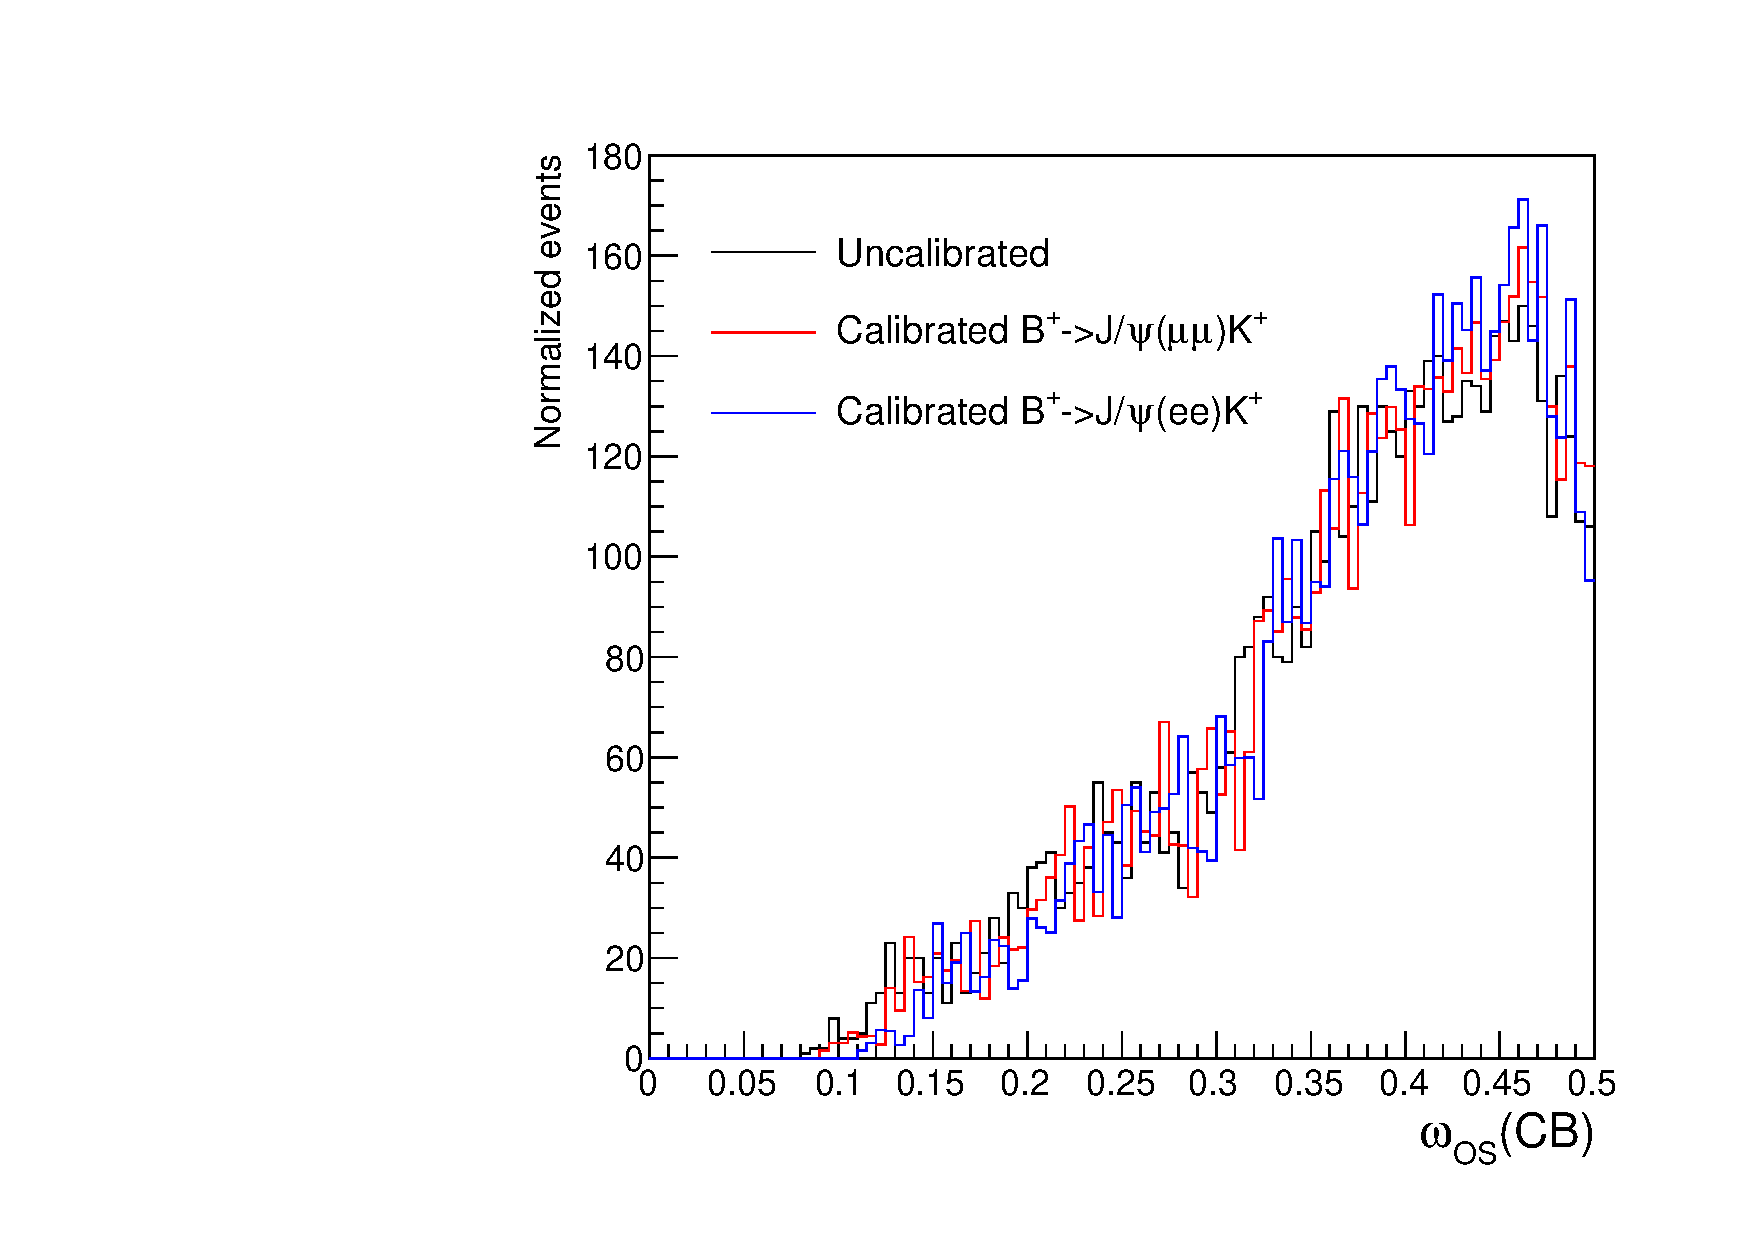
\includegraphics[width=0.6\linewidth]{Tagging/omega_Bu2JpsieeK_Bu2JpsiMuMuK_OS_fullRun1.pdf}
     \vspace*{-0.5cm}
  \end{center}
    \caption{
   The OS mistag distributions for $\Bs\to\jpsi\phi$ signal events before (black) and after the calibration on $\Bp\to\jpsi(\mumu)\Kp$ (red) and $\Bp\to\jpsi(\epem)\Kp$ (blue).}
  \label{fig:MistagOS} 
\end{figure}

 \begin{table}[htb]
  \caption{
   The parameters used in Eq.~\ref{eq:mistag} to calibrate the per-event mistag probabilities for OS calibration. When two uncertainties are quoted, the first one is statistical and the second one is systematic.}
    \small{
\begin{center}\begin{tabular}{ccc}
    Parameter                         &  $\Bp\to\jpsi(\mumu)\Kp$  & \Bp\to\jpsi(\mumu)\Kp  \\ 
    \hline
    $\langle\eta\rangle$ & 0.3751 &    0.3789 \\
    $p_{0}-\langle\eta\rangle$ &   0.0062$\pm$0.0019$\pm$0.0040 & 0.0086$\pm$0.0021 \\
    $\Delta p_{0}/2$& 0.0070$\pm$0.0006 &    0.0083$\pm$0.0021 \\
    $p_{1}$ &   0.982$\pm$0.007$\pm$0.034 & 0.931$\pm$0.021 \\
    $\Delta p_{1}/2$& 0.033$\pm$0.006 &    0.0115$\pm$0.0205 \\
    \hline
  \end{tabular}\end{center}
  }
\label{tab:CalibrationFTOS}
\end{table}

The $\Bs\to\jpsi(\epem)\phi$ dataset is divided in four independent subsamples as described in Sec.~\ref{sec:FlavTagg}. The fractions, the efficiencies, and the tagging powers calculated for OS calibration on $\Bp\to\jpsi(\mumu)\Kp$ and $\Bp\to\jpsi(\epem)\Kp$ as measured for $\Bs\to\jpsi(\epem)\phi$ signal candidates from full 2011 and 2012 datasets and from full simulation sample are reported in Table~\ref{tab:FTperformanceRDfull},~\ref{tab:FTperformanceRDfullOS} and Table~\ref{tab:FTperformanceMCfull},~\ref{tab:FTperformanceMCfullOS}, respectively. The total tagging efficiency and tagging power of data sample are (75.70$\pm$0.68)$\%$ and (5.20$\pm$0.10)$\%$ with OS calibration on muon mode of $\Bp\to\jpsi\Kp$ and (75.80$\pm$0.68)$\%$ and (4.98$\pm$0.10)$\%$ for OS calibration on $\Bp\to\jpsi\Kp$ with electron final state. In case of simulated data, the total tagging efficiency and tagging power are (74.73$\pm$0.13)$\%$ and (5.38$\pm$0.02)$\%$ with OS calibration on $\Bp\to\jpsi(\mumu)\Kp$ and (74.90$\pm$0.13)$\%$ and (5.17$\pm$0.02)$\%$ with OS calibration on $\Bp\to\jpsi(\epem)\Kp$ decay. The flavour tagging perfromance calculated for OS calibration on electron mode of $\Bp\to\jpsi\Kp$ slightly decreases the tagging performance of $\Bs\to\jpsi(\epem)\phi$ signal events. It is considered as a source of systematic uncertainty in Sec.~\ref{subsec:Syst:FT}. 

\begin{table}[htb]
  \caption{
   The summary of the tagging efficiency ($\varepsilon$), square dilution factor ($\mathcal{D}^{2}$) and tagging power ($\varepsilon\mathcal{D}^{2}$) for the different categories of tagger, obtained from $\Bs\to\jpsi(\epem)\phi$ {\bf signal candidates from full 2011 and 2012 data samples} after the OS tagging calibration on $\Bs\to\jpsi(\epem)\phi$ has been applied. The column "Fraction" reports the fraction of events in each category out of the all tagged events.}
    \small{
\begin{center}\begin{tabular}{ccccc}
   \hline
    Category & Fraction($\%$)&$\varepsilon(\%)$ & $\mathcal{D}^{2}$ & $\varepsilon\mathcal{D}^{2}(\%)$\\
  \hline
    OS-only& 17.1 &12.98$\pm$0.32 &  0.0901$\pm$0.0024 & 1.17$\pm$0.05 \\
     SSK-only& 51.5 &39.06$\pm$0.46 & 0.0315$\pm$0.0013  & 1.23$\pm$0.04 \\
     OS$\&$SSK& 31.4 &23.76$\pm$0.40 &  0.1086$\pm$0.0020 & 2.58$\pm$0.08 \\
    \hline
     Total& 100 &75.80$\pm$0.68 & 0.0657$\pm$0.0033& 4.98$\pm$0.10 \\
    \hline
    \end{tabular}\end{center}
  }
\label{tab:FTperformanceRDfullOS}
\end{table}

\begin{table}[htb]
  \caption{
   The summary of the tagging efficiency ($\varepsilon$), square dilution factor ($\mathcal{D}^{2}$) and tagging power ($\varepsilon\mathcal{D}^{2}$) for the different categories of tagger, obtained from $\Bs\to\jpsi(\epem)\phi$ {\bf signal candidates from full simulated data sample} after the OS tagging calibration on $\Bs\to\jpsi(\epem)\phi$ has been applied. The column "Fraction" reports the fraction of events in each category out of the all tagged events. }
    \small{
\begin{center}\begin{tabular}{ccccc}
   \hline
    Category & Fraction($\%$)&$\varepsilon(\%)$ & $\mathcal{D}^{2}$ & $\varepsilon\mathcal{D}^{2}(\%)$\\
  \hline
    OS-only& 16.9 &12.65$\pm$0.06 &  0.0917$\pm$0.0006 &  1.16$\pm$0.01 \\
     SSK-only& 55.7&40.03$\pm$0.09 &  0.0347$\pm$0.0003 &  1.39$\pm$0.01 \\
     OS$\&$SSK& 27.4&22.22$\pm$0.07 &  0.1179$\pm$0.0005 &  2.62$\pm$0.02 \\
    \hline
     Total& 100 &74.90$\pm$0.13 & 0.0690$\pm$0.0008 & 5.17$\pm$0.02 \\
    \hline
    \end{tabular}\end{center}
  }
\label{tab:FTperformanceMCfullOS}
\end{table}

\clearpage

\section{Results of likelihood fit}\label{sec:Results}

Table~\ref{tab:FitResults} shows the $\Bs\to\jpsi(\epem)\phi$ final results of the fit to 3~$\invfb$ of LHCb dataset including decay time and angular acceptance effect, decay time resolution and fixed flavour tagging calibration. A blind string has been applied in the fit for $\Gs$, $\DGs$ and $\phis$. The correlation matrix of the fit is shown in Table~\ref{tab:CorrelationMatrix}. The projections of the fit result on the decay time and helicity angle distributions are shown in Fig.~\ref{fig:TimeAngleFit} ({\tt Preliminary}).

\begin{table}[htb]
  \caption{
   The results of the unbinned maximum likelihood fit to the selected $\Bs\to\jpsi(\epem)\phi$ candidates including all acceptance and resolution effects. The tagging calibration parameters and $\dms$ are Gaussian constrained in the fit. The values for $\Gs$, $\DGs$ and $\phis$ are blinded. The uncertainty is statistical. {\tt Preliminary}}
    \small{
\begin{center}\begin{tabular}{cc}
Parameter & Fit result and error \\ 		\hline
            $\Gamma_{s}$ [$\ps^{-1}$] &       $X.XXX \pm$ 0.0057                \\
      $\Delta\Gamma_{s}$ [$\ps^{-1}$]&         $X.XXX \pm$  0.0155                \\
$A_{\hspace{-1pt}\perp}^{2}$ &      0.2750 $\pm$   0.0121                \\
             $A_0^2$ &      0.5025 $\pm$  0.0088                \\
  $\delta_\parallel$ [$\rad$] &       3.0092 $\pm$    0.1759                \\
      $\delta_\perp$ [$\rad$] &          3.1086 $\pm$    0.3686                \\
               $F_S$ &     0.0735 $\pm$   0.0167                \\
          $\delta_S$ [$\rad$] &     -0.1093 $\pm$   0.0801                \\
            $\phi_s$ [$\rad$] &      $X.XXX \pm$    0.1548                \\
           $\lambda$ &      0.9836 $\pm$   0.0261                \\
           $\Delta m_s$~[ps$^{-1}$] &       18.176 $\pm$    0.147                \\
\hline
\end{tabular}\end{center}
  }
\label{tab:FitResults}
\end{table}

\begin{sidewaystable}[htb]
  \caption{
   the statistical correlation matrix from nominal fit. {\tt Preliminary}
}
    \small{
\begin{center}\begin{tabular}{@{}|l|r|r|r|r|r|r|r|r|r|r|r|r|r|r|r|@{}}
\hline
& $\Gamma$ & $\Delta\Gamma$ & $A_{\hspace{-1pt}\perp}^{2}$ & $A_0^2$ & $\delta_\parallel$ & $\delta_\perp$ & $F_S$ & $\delta_S$ & $\Delta m_s$ & $\phi_s$ & $\lambda$ & $\omega_{P1}^{OS}$ & $\omega_{P0}^{OS}$ & $\omega_{P1}^{SS}$ & $\omega_{P0}^{SS}$\\ \hline \hline
$\Gamma$ & 1.00 & -0.31 & 0.22 & -0.18 & 0.02 & 0.01 & 0.13 & 0.02 & 0.01 & 0.03 & 0.02 & -0.00 & 0.00 & -0.00 & 0.00 \\
$\Delta\Gamma$ &  & 1.00 & \bf{-0.54} & \bf{0.52} & -0.00 & 0.01 & -0.14 & -0.02 & 0.01 & -0.01 & -0.02 & 0.00 & -0.00 & 0.00 & -0.00 \\
$A_{\hspace{-1pt}\perp}^{2}$ &  &  & 1.00 & \bf{-0.52} & 0.17 & 0.06 & 0.01 & 0.02 & 0.03 & 0.04 & 0.04 & -0.00 & -0.00 & -0.00 & 0.00 \\
$A_0^2$ &  &  &  & 1.00 & 0.02 & -0.01 & -0.00 & 0.00 & -0.01 & -0.03 & 0.00 & 0.00 & 0.00 & 0.00 & -0.00 \\
$\delta_\parallel$ &  &  &  &  & 1.00 & 0.21 & 0.08 & 0.00 & 0.06 & 0.02 & 0.14 & -0.01 & -0.01 & -0.02 & 0.02 \\
$\delta_\perp$ &  &  &  &  &  & 1.00 & 0.01 & -0.02 & \bf{0.79} & 0.39 & 0.19 & -0.02 & -0.01 & 0.01 & 0.02 \\
$F_S$ &  &  &  &  &  &  & 1.00 & 0.17 & 0.06 & 0.06 & 0.14 & -0.02 & 0.04 & -0.02 & 0.02 \\
$\delta_S$ &  &  &  &  &  &  &  & 1.00 & 0.10 & 0.06 & 0.05 & -0.01 & 0.00 & -0.00 & 0.01 \\
$\Delta m_s$ &  &  &  &  &  &  &  &  & 1.00 & 0.47 & 0.17 & -0.02 & -0.01 & 0.02 & 0.02 \\
$\phi_s$ &  &  &  &  &  &  &  &  &  & 1.00 & 0.05 & -0.05 & -0.02 & -0.01 & -0.02 \\
$\lambda$ &  &  &  &  &  &  &  &  &  &  & 1.00 & -0.01 & 0.01 & -0.00 & 0.00 \\
$\omega_{P1}^{OS}$ &  &  &  &  &  &  &  &  &  &  &  & 1.00 & 0.00 & 0.00 & -0.00 \\
$\omega_{P0}^{OS}$ &  &  &  &  &  &  &  &  &  &  &  &  & 1.00 & -0.00 & 0.00 \\
$\omega_{P1}^{SS}$ &  &  &  &  &  &  &  &  &  &  &  &  &  & 1.00 & 0.07 \\
$\omega_{P0}^{SS}$ &  &  &  &  &  &  &  &  &  &  &  &  &  &  & 1.00 \\
\hline
\end{tabular}\end{center}
  }
\label{tab:CorrelationMatrix}
\end{sidewaystable}

\begin{figure}
  \begin{center}
    \begin{minipage}[ht!]{0.48\linewidth}
  \includegraphics[width=1.\linewidth]{Fit_phis/Overlay_time_All_SubSets.pdf} \\
  \includegraphics[width=1.\linewidth]{Fit_phis/Overlay_helcosthetaK_All_SubSets.pdf} \\
 \end{minipage}
 \hfill
    \vspace{-5mm}
  \begin{minipage}[ht!]{0.48\linewidth}
 \includegraphics[width=1.\linewidth]{Fit_phis/Overlay_helcosthetaL_All_SubSets.pdf} \\ 
 \includegraphics[width=1.\linewidth]{Fit_phis/Overlay_helphi_All_SubSets.pdf} \\
     \end{minipage}
     \vspace*{-0.5cm}
  \end{center}
    \caption{
   The decay time and helicity-angle distributions for $\Bs\to\jpsi(\epem)\phi$ reconstructed candidates (data points) with the one-dimensional projections of the PDF at the maximum likelihood fit. The solid blue line shows the total signal contribution, which is composed of $CP$-even (long dashed red), $CP$-odd (short-dashed green) and S-wave (dash-dotted purple) (not seen) contributions. {\tt Preliminary.}}  
  \label{fig:TimeAngleFit} 
\end{figure}

\clearpage

\section{Systematic uncertainties}\label{sec:SystUnc}

All systematics are described below and a summary is reported in Table~\ref{tab:StatError}. The tagging parameters are allowed to float in the fit (Gaussian constrained within their uncertainty) and thus the systematic uncertainties due to those is propagated into the statistical uncertainties reported on physics parameters.

\subsection{$M(\jpsi(\epem)\phi)$ mass model}

{\it To calculate a new set of event weights obtained from new $M(\jpsi(\epem)\phi)$ fit model.}

\subsection{Angular acceptance}

{\it To add the description of iterative weighting method.}

\subsection{Angular resolution}\label{subsec:Syst:AngRes}

{\it To add the toy studies of the angular resolution.}

\subsection{Decay time resolution}


\subsection{Trigger efficiency}


\subsection{Flavour tagging}\label{subsec:Syst:FT}

{\it The difference between tagging parameters obtained from OS calibration on $\Bp\to\jpsi(\mumu)\Kp$ and $\Bp\to\jpsi(\epem)\Kp$ is assigned as the systematic uncertainty. }


\subsection{Length and momentum scale}

The uncertainty on the LHCb length scale is estimated to be at most 0.020$\%$~\cite{LHCb:ANA-2012-053}, which translates directly in an uncertainty on $\Gs$, $\DGs$ and $\dms$ of 0.020$\%$ with other parameters being unaffected. The momentum scale uncertainty is at most 0.022$\%$~\cite{LHCb:ANA-2012-053}. As it affects both the reconstructed momentum and mass of the $\Bs$ meson, it cancels to a large extent and the resulting effect on $\Gs$ and $\DGs$ is negligible.

\subsection{Contribution from $\Lb$ decays}


\subsection{Fit bias}

{\it A possible bias of the fitting procedure is investigated by generating and fitting many simulated pseudo-experiments of equivalent size to the data sample, generated with physics parameters close to those obtained in the nominal fit.}

\subsection{Further checks}

{\it Additional checks will perform by repeating the nominal fit to data in bins of year of data taking, magnet polarity.}

 
\begin{table}[htb]
  \caption{
   Statistical and systematic uncertainties. The uncertainty for $\phis$ from the fit bias will need to be re-evaluated post-unblinding.
}
    \small{
\begin{center}
\begin{adjustwidth}{-1.5cm}{}
\begin{tabular}{ccccccccc}
Source &$\Gs$ [$\ps^{-1}$]&$\DGs$ [$\ps^{-1}$]&$A_{\hspace{-1pt}\perp}^{2}$&$A_0^2$&$\delta_\parallel$ [$\rad$]&$\delta_\perp$ [$\rad$]&$\phi_s$ [$\rad$]&$\lambda$\\ 		\hline
 Stat. uncert.       &  0.0057    & 0.0155&0.0121&0.0088&0.1759&0.3686&0.1548&0.0261                \\
 \hline
 Mass model      &         &&&&&&&               \\
 Ang. acc.&      &&&&&&&                \\
 Ang. resol.&      &&&&&&&                \\
 Time resol.&      &&&&&&&                \\
 Trigger eff. &      &&&&&&&                \\
 Flav. tag. &  &&&&&&&                \\
 Length, mom. scales&      &&&&&&&                \\
 $\Lb$ background&      &&&&&&&                \\
 Fit bias&      &&&&&&&                \\
 \hline
 Quad. sum of syst.&      &&&&&&&                \\
 Total uncertainties&      &&&&&&&                \\
 \hline
\end{tabular}
\end{adjustwidth}
\end{center}
  }
\label{tab:StatError}
\end{table}

\clearpage

\section{Conclusion}\label{sec:Concl}

We have presented the tagged, time dependent angular analysis of 11 645$\pm$114 $\Bs\to\jpsi(\epem)\phi$ signal candidates with $\jpsi\to\epem$ and in the $M(\Kp\Km)$ region around the $\phi(1020)$ meson. These were recorded in 3~$\invfb$ of $pp$ collision data collected by the $\lhcb$ detector during 2011 and 2012 years. The effective decay time resolution and effective tagging power are 50.2~$\fs$ and 5.2$\%$, respectively. The analysis provides access to a number of different physics parameters including the CP-violating phase, average decay width and decay width difference of the $\Bs$ system as well as the transversely amplitudes and strong phases of the decay. The final results are reported in Table~\ref{tab:FitResultsConcl}. This is the first measurement of the $CP$ content of the $\Bs\to\jpsi(\epem)\phi(\Kp\Km)$ decay and first time that $\phis$ and $\DGs$ have been measured in final state containing the $\jpsi\to\epem$ decay. These measurements will contribute to increased precision in the global average of the $\Bs$ mixing parameters.

\begin{table}[htb]
  \caption{
   The results of the unbinned maximum likelihood fit to the selected $\Bs\to\jpsi(\epem)\phi$ candidates including all acceptance and resolution effects. The tagging calibration parameters and $\dms$ are Gaussian constrained in the fit. The values for $\DGs$ and $\phis$ are blinded. The uncertainty is statistical.
}
    \small{
\begin{center}\begin{tabular}{cc}
Parameter & Fit result and error \\ 		\hline
            $\Gamma_{s}$ [$\ps^{-1}$] &       $X.XXX \pm$ 0.0057                \\
      $\Delta\Gamma_{s}$ [$\ps^{-1}$]&         $X.XXX \pm$  0.0155                \\
$A_{\hspace{-1pt}\perp}^{2}$ &      0.2750 $\pm$   0.0121                \\
             $A_0^2$ &      0.5025 $\pm$  0.0088                \\
  $\delta_\parallel$ [$\rad$] &       3.0092 $\pm$    0.1759                \\
      $\delta_\perp$ [$\rad$] &          3.1086 $\pm$    0.3686                \\
               $F_S$ &     0.0735 $\pm$   0.0167                \\
          $\delta_S$ [$\rad$] &     -0.1093 $\pm$   0.0801                \\
            $\phi_s$ [$\rad$] &      $X.XXX \pm$    0.1548                \\
           $\lambda$ &      0.9836 $\pm$   0.0261                \\
           $\Delta m_s$~[ps$^{-1}$] &       18.176 $\pm$    0.147                \\
\hline
\end{tabular}\end{center}
  }
\label{tab:FitResultsConcl}
\end{table}
\clearpage

\section{To-do list}
\begin{enumerate}
 \item Add comparison plots of kinematic variables for $\Bs\to\jpsi(\mumu)\phi$ and $\Bs\to\jpsi(\epem)\phi$
 \item Complete systematic studies
 \item Perform final fit projections of the decay time and helicity angle 
\end{enumerate}
\clearpage

% \section{Layout}

\begin{enumerate}

\item Unnecessary blank space should be avoided, between paragraphs or
  around figures and tables.

\item Figure and table captions should be concise and use a somewhat smaller typeface
  than the main text, to help distinguish them. This is achieved by 
  inserting \verb!\small! at the beginning of the caption.
  (NB with the latest version of the file \verb!premable.tex! this is automatic)
  Figure captions go below the figure, table captions go above the
  table.

\item Captions and footnotes should be punctuated correctly, like
  normal text. The use of too many footnotes should be avoided:
  typically they are used for giving commercial details of companies,
  or standard items like coordinate system definition or the implicit
  inclusion of charge-conjugate processes.\footnote{If placed at the end
    of a sentence, the footnote symbol normally follows the
    punctuation; if placed in the middle of an equation, take care to
    avoid any possible confusion with an index.}$^,$\footnote{The standard footnote reads: The inclusion of charge-conjugate processes is implied.}

\item Tables should be formatted in a simple fashion, without
  excessive use of horizontal and vertical lines. See
  Table~\ref{tab:example} for an example.

\item Figures and tables should normally be placed so that they appear
  on the same page as their first reference, but at the top or bottom
  of the page; if this is not possible, they should come as soon as
  possible afterwards.  They must all be referred to from the text.

\item If one or more equations are referenced, all equations should be numbered using parentheses as shown in
  Eq.~\ref{eq:CKM},
  \begin{equation}
    \label{eq:CKM}
    V_{\uquark\squark}V_{\uquark\bquark}^* + 
    V_{\cquark\squark}V_{\cquark\bquark}^* + 
    V_{\tquark\squark}V_{\tquark\bquark}^* = 0 \ . 
  \end{equation}
  
\item Displayed results like
  \begin{equation*}
    \BF(\decay{\Bs}{\mumu}) < 1.5 \times 10^{-8} \text{ at 95\% CL}
  \end{equation*}
  should in general not be numbered.

\item Numbered equations should be avoided in captions and footnotes.

\item Displayed equations are part of the normal grammar of the
  text. This means that the equation should end in full stop or comma if
  required when reading aloud. The line after the equation should only
  be indented if it starts a new paragraph.

\item Sub-sectioning should not be excessive: sections with more than three
levels of index (1.1.1) should be avoided.

%\item It is generally preferable to itemize a list using numbers rather
%than bullets.

\item Acronyms should be defined the first time they are used,
  \eg ``Monte Carlo~(MC) events containing a doubly
  Cabibbo-suppressed~(DCS) decay have been generated.''
  The abbreviated words should not be capitalised if it is not naturally
  written with capitals, \eg quantum chromodynamics (QCD),
  impact parameter (IP), boosted decision tree (BDT).
  Avoid acronyms if they are used three times or less.
  A sentence should never start with an acronym and its better to
  avoid it as the last word of a sentence as well.

\end{enumerate}

\begin{table}[t]
  \caption{
    %\small %captions should be a little bit smaller than main text
    Background-to-signal ratio estimated in a $\pm 50\mevcc$ 
    mass window for the prompt and long-lived backgrounds, and the 
    minimum bias rate.}
\begin{center}\begin{tabular}{lccc}
    \hline
    Channel                           & $B_{\mathrm{pr}}/S$ & $B_{\mathrm{LL}}/S$   & MB rate       \\ 
    \hline
    \BsToJPsiPhi              & $ 1.6 \pm 0.6$ & $ 0.51 \pm 0.08$ & $\sim 0.3$ Hz \\
    \BdToJPsiKst              & $ 5.2 \pm 0.3$ & $1.53 \pm 0.08 $ & $\sim 8.1$ Hz \\
    \decay{\Bp}{\jpsi\Kstarp} & $ 1.6 \pm 0.2$ & $0.29 \pm 0.06$  & $\sim 1.4$ Hz \\
    \hline
  \end{tabular}\end{center}
\label{tab:example}
\end{table}

% old table with vertical lines
%\begin{table}[t]
%  \caption{
%    \small %captions should be a little bit smaller than main text
%    Background-to-signal ratio estimated in a $\pm 50\mevcc$ 
%    mass window for the prompt and long-lived backgrounds, and the 
%    minimum bias rate.}
%\begin{center}\begin{tabular}{l|c|c|c}
%    Channel                           & $B_{\mathrm{pr}}}/S$ & $B_{{\mathrm{LL}}/S$   & MB rate       \\ 
%    \hline
%    \BsToJPsiPhi              & $ 1.6 \pm 0.6$ & $ 0.51 \pm 0.08$ & $\sim 0.3$ Hz \\
%    \BdToJPsiKst              & $ 5.2 \pm 0.3$ & $1.53 \pm 0.08 $ & $\sim 8.1$ Hz \\
%    \decay{\Bp}{\jpsi\Kstarp} & $ 1.6 \pm 0.2$ & $0.29 \pm 0.06$  & $\sim 1.4$ Hz \\
%  \end{tabular}\end{center}
%\label{tab:example}
%\end{table}


% \section{Typography}
\label{sec:typography}

The use of the Latex typesetting symbols defined in the file
\texttt{lhcb-symbols-def.tex} and detailed in the appendices of this
document is strongly encouraged as it will make it much easier to
follow the recommendation set out below.

\begin{enumerate}

\item \lhcb is typeset with a normal (roman) lowercase b.

\item Titles are in bold face, and usually only the first word is
  capitalised.

\item Mathematical symbols and particle names should also be typeset
  in bold when appearing in titles.

\item Units are in roman type, except for constants such as $c$ or $h$
  that are italic: \gev, \gevcc.  The unit should be separated from
  the value with a thin space (``\verb!\,!''),
  and they should not be broken over two lines.
  Correct spacing is automatic when using predefined units inside math mode: \verb!$3.0\gev$! $\to 3.0\gev$.
  Spacing goes wrong when using predefined units outside math mode AND forcing extra space:
  \verb!3.0\,\gev! $\to$ 3.0\,\gev or worse:   \verb!3.0~\gev! $\to$ 3.0~\gev. 

\item  If factors of $c$ are kept, they should be used both for masses and
  momenta, \eg $p=5.2\gevc$ (or $\gev c^{-1}$), $m = 3.1\gevcc$ (or $\gev c^{-2}$). If they are dropped this
  should be done consistently throughout, and a note should be added
  at the first instance to indicate that units are taken with $c=1$.

\item The \% sign should not be separated from the number that precedes it: 5\%, not 5 \%. 
A thin space is also acceptable: 5\,\%, but should be applied consistently throughout the paper.

\item Ranges should be formatted consistently. The recommendend form is to use a dash with no spacing around it: 
7--8\gev, obtained as \verb!7--8\gev!. 

\item Italic is preferred for particle names (although roman is
  acceptable, if applied consistently throughout).  Particle Data
  Group conventions should generally be followed: \Bd (no need for a
  ``d'' subscript), \decay{\Bs}{\jpsi\phi}, \Bsb,
  (note the long bar, obtained with \verb!\overline!, in contrast to the discouraged short \verb!\bar{B}! resulting in $\bar{B}$), \KS (note the
  uppercase roman type ``S''). 
This is most easily achieved by using the predefined symbols described in 
  Appendix~\ref{sec:listofsymbols}.
  Unless there is a good reason not to, the charge of a particle should be
  specified if there is any possible ambiguity 
  ($m(\Kp\Km)$ instead of $m(KK)$, which could refer to neutral kaons).

\item Decay chains can be written in several ways, depending on the complexity and the number of times it occurs. Unless there is a good reason not to, usage of a particular type should be consistent within the paper.
Examples are: 
$\Dsp\to\phi\pip$, with $\phi\to\Kp\Km$; 
$\Dsp\to\phi\pip$ ($\phi\to\Kp\Km$);  
$\Dsp\to\phi(\to\Kp\Km)\pip$; or
$\Dsp\to[\Kp\Km]_\phi\pip$.



\item Variables are usually italic: $V$ is a voltage (variable), while
  1 V is a volt (unit). Also in combined expressions: $Q$-value, $z$-scale, $R$-parity \etc

\item Subscripts and superscripts are roman type when they refer to a word (such as T
  for transverse) and italic when they refer to a variable (such as
  $t$ for time): \pt, \dms, $t_{\mathrm{rec}}$.

\item Standard function names are in roman type: \eg $\cos$, $\sin$
  and $\exp$.

\item Figure, Section, Equation, Chapter and Reference should be
  abbreviated as Fig., Sect. (or alternatively Sec.), Eq., Chap.\ and
  Ref.\ respectively, when they refer to a particular (numbered) item,
  except when they start a sentence. Table and Appendix are not
  abbreviated.  The plural form of abbreviation keeps the point after
  the s, \eg Figs.~1 and~2. Equations may be referred to either with 
  (``Eq.~(1)'') or without (``Eq.~1'') parentheses, 
  but it should be consistent within the paper.

\item Common abbreviations derived from Latin such as ``for example''
  (\eg), ``in other words'' (\ie), ``and so forth'' (\etc), ``and
  others'' (\etal), ``versus'' (\vs) can be used, with the typography
  shown, but not excessively; other more esoteric abbreviations should be avoided.
  

\item Units, material and particle names are usually lower case if
  spelled out, but often capitalised if abbreviated: amps (A), gauss
  (G), lead (Pb), silicon (Si), kaon (\kaon), but proton (\proton).

%\item The prefix for 1000 (k, \eg kV) should not be confused with
%  that used in computing (K, which strictly speaking denotes $2^{10}$,
%  \eg KB).

\item Counting numbers are usually written in words if they start a
  sentence or if they have a value of ten or below in descriptive
  text (\ie not including figure numbers such as ``Fig.\ 4'', or
  values followed by a unit such as ``4\,cm'').
  The word 'unity' can be useful to express the special meaning of
  the number one in expressions such as: 
``The BDT output takes values between zero and unity''.
% Numbers should not be
%  written as words if they by nature are real numbers that happen to
%  take an integer value, such as $\chisq/\mathrm{ndf} < 4$.

\item Numbers larger than 9999 have a comma (or a small space, but not both) between
  the multiples of thousand: \eg 10,000 or 12,345,678.  The decimal
  point is indicated with a point rather than a comma: \eg 3.141.

\item We apply the rounding rules of the
  PDG~\cite{PDG2014}. The basic rule states that if the three
  highest order digits of the uncertainty lie between 100 and 354, we round
  to two significant digits. If they lie between 355 and 949, we round
  to one significant digit. Finally, if they lie between 950 and 999,
  we round up and keep two significant digits. In all cases,
  the central value is given with a precision that matches that of the
  uncertainty. So, for example, the result $0.827 \pm 0.119$ should be
  written as $0.83\pm 0.12$, $0.827\pm 0.367$ should turn into
  $0.8\pm 0.4$, and $14.674\pm0.964$ becomes $14.7\pm1.0$.
 When writing numbers with uncertainty components from
  different sources, \ie statistical and systematic uncertainties, the rule
  applies to the uncertainty with the best precision, so $0.827\pm
  0.367\stat\pm 0.179\syst$ goes to $0.83\pm 0.37\stat\pm 0.18\syst$ and
  $8.943\pm 0.123\stat\pm 0.995\syst$ goes to $8.94\pm 0.12\stat\pm
  1.00\syst$.

\item When rounding numbers, it should be avoided to pad with zeroes
  at the end. So $51237 \pm 4561$ should be rounded as $(5.12 \pm 0.46)
  \times 10^4$ and not $51200 \pm 4600$.

\item When rounding numbers in a table, some variation of the rounding
  rules above may be required to achieve uniformity.

\item Hyphenation should be used where necessary to avoid ambiguity,
  but not excessively. For example: ``big-toothed fish''
  (to indicate that big refers to the teeth, not to the fish),
  but ``big white fish''.
  A compound modifier often requires hyphenation 
  (\CP-violating observables, \bquark-hadron decays, final-state radiation, second-order polynomial),
  even if the same combination in an adjective-noun combination does not
  (direct \CP violation, heavy \bquark hadrons, charmless final state).
  Adverb-adjective combinations are not hyphenated if the adverb ends with 'ly':
  oppositely charged pions, kinematically similar decay.
  Cross-section, cross-check, and two-dimensional are hyphenated.
  Semileptonic, pseudorapidity, pseudoexperiment, multivariate, multidimensional, reweighted, preselection, 
  nonresonant, nonzero, nonparametric, nonrelativistic, misreconstructed and misidentified
  are single words and should not be hyphenated.

\item Minus signs should be in a proper font ($-1$), not just hyphens
  (-1); this applies to figure labels as well as the body of the text.
  In Latex, use math mode (between \verb!$$!'s) or make a dash (``\verb!--!'').
  In ROOT, use \verb!#font[122]{-}! to get a normal-sized minus sign. 

\item Inverted commas (around a title, for example) should be a
  matching set of left- and right-handed pairs: ``Title''. The use of
  these should be avoided where possible.

\item Single symbols are preferred for variables in equations, \eg\
  \BF\ rather than BF for a branching fraction.

\item Parentheses are not usually required around a value and its
  uncertainty, before the unit, unless there is possible ambiguity: so
  $\dms = 20 \pm 2\invps$ does not need parentheses, whereas $f_d =
  (40 \pm 4)$\% or $x=(1.7\pm0.3)\times 10^{-6}$ does.
  The unit does not need to be repeated in
  expressions like $1.2 < E < 2.4\gev$.

\item The same number of decimal places should be given for all values
  in any one expression (\eg $5.20 < m_B < 5.34\gevcc$).

\item Apostrophes are best avoided for abbreviations: if the abbreviated term
  is capitalised or otherwise easily identified then the plural can simply add
  an s, otherwise it is best to rephrase: \eg HPDs, \pizs, pions, rather
  than HPD's, \piz's, $\pion$s.

\item Particle labels, decay descriptors and mathematical functions are not nouns, and need often to be followed by a noun. 
Thus ``background from $\Bd\to\pi^+\pi^-$ decays'' instead of ``background from $\Bd\to\pi^+\pi^-$'',
and ``the width of the Gaussian function'' instead of ``the width of the Gaussian''.

\item In equations with multidimensional integrations or differentiations, the differential terms should be separated by a thin space. 
Thus $\int f(x,y) dx\,dy$ instead $\int f(x,y) dxdy$ and
$\frac{d^2\Gamma}{dx\,dQ^2}$ instead of $\frac{d^2\Gamma}{dxdQ^2}$.
The d's are allowed in either roman or italic font, but should be consistent throughout the paper.


\end{enumerate}


% \section{Detector and simulation}
\label{sec:Detector}
The following paragraph can be used for the detector
description. Modifications may be required in specific papers to fit
within page limits, to enhance particular detector elements or to
introduce acronyms used later in the text.
References to the individual detector performance papers are marked with 
a \verb!*!
and should only be included if the analysis relies on numbers or methods 
described in the specific papers. Otherwise, a reference to the overall 
detector performance paper~\cite{LHCb-DP-2014-002} will suffice.

The \lhcb detector~\cite{Alves:2008zz,LHCb-DP-2014-002} is a single-arm forward
spectrometer covering the \mbox{pseudorapidity} range $2<\eta <5$,
designed for the study of particles containing \bquark or \cquark
quarks. The detector includes a high-precision tracking system
consisting of a silicon-strip vertex detector surrounding the $pp$
interaction region~\cite{LHCb-DP-2014-001}\verb!*!, a large-area silicon-strip detector located
upstream of a dipole magnet with a bending power of about
$4{\mathrm{\,Tm}}$, and three stations of silicon-strip detectors and straw
drift tubes~\cite{LHCb-DP-2013-003}\verb!*! placed downstream of the magnet.
The tracking system provides a measurement of momentum, \ptot, of charged particles with
a relative uncertainty that varies from 0.5\% at low momentum to 1.0\% at 200\gevc.
The minimum distance of a track to a primary vertex, the impact parameter, is measured with a resolution of $(15+29/\pt)\mum$,
where \pt is the component of the momentum transverse to the beam, in\,\gevc.
Different types of charged hadrons are distinguished using information
from two ring-imaging Cherenkov detectors~\cite{LHCb-DP-2012-003}\verb!*!. 
Photons, electrons and hadrons are identified by a calorimeter system consisting of
scintillating-pad and preshower detectors, an electromagnetic
calorimeter and a hadronic calorimeter. Muons are identified by a
system composed of alternating layers of iron and multiwire
proportional chambers~\cite{LHCb-DP-2012-002}\verb!*!.
The online event selection is performed by a trigger~\cite{LHCb-DP-2012-004}\verb!*!, 
which consists of a hardware stage, based on information from the calorimeter and muon
systems, followed by a software stage, which applies a full event
reconstruction.

A more detailed description of the 'full event reconstruction' could be:
\begin{itemize}
\item The trigger~\cite{LHCb-DP-2012-004}\verb!*! consists of a
hardware stage, based on information from the calorimeter and muon
systems, followed by a software stage, in which all charged particles
with $\pt>500(300)\mev$ are reconstructed for 2011 (2012) data.
For triggers that require neutral particles, 
energy deposits in the electromagnetic calorimeter are 
analysed to reconstruct \piz and $\gamma$ candidates.
\end{itemize}

The trigger description has to be specific for the analysis in
question. In general, you should not attempt to describe the full
trigger system. Below are a few variations that inspiration can be
taken from. First from a hadronic analysis, and second from an
analysis with muons in the final state.
A detailed description of the trigger conditions for Run 1 is available in Ref.~\cite{LHCb-PUB-2014-046}.
\begin{itemize}
\item At the hardware trigger stage, events are required to have a muon with high \pt or a
  hadron, photon or electron with high transverse energy in the calorimeters. For hadrons,
  the transverse energy threshold is 3.5\gev.
  The software trigger requires a two-, three- or four-track
  secondary vertex with a significant displacement from the primary
  $pp$ interaction vertices~(PVs). At least one charged particle
  must have a transverse momentum $\pt > 1.7\gevc$ and be
  inconsistent with originating from a PV.
  A multivariate algorithm~\cite{BBDT} is used for
  the identification of secondary vertices consistent with the decay
  of a \bquark hadron.
%\item The software trigger requires a two-, three- or four-track
%  secondary vertex with a large sum of the transverse momentum, \pt, of
%  the tracks and a significant displacement from the primary $pp$
%  interaction vertices~(PVs). At least one track should have $\pt >
%  1.7\gevc$ and \chisqip with respect to any
%  primary interaction greater than 16, where \chisqip is defined as the
%  difference in \chisq of a given PV reconstructed with and
%  without the considered track.\footnote{If this sentence is used to define \chisqip
%  for a composite particle instead of for a single track, replace ``track'' by ``particle'' or ``candidate''}
% A multivariate algorithm~\cite{BBDT} is used for
%  the identification of secondary vertices consistent with the decay
%  of a \bquark hadron.
\item Candidate events are first required to pass the hardware trigger,
  which selects muons with a transverse momentum $\pt>1.48\gevc$ 
  in the 7\tev data or $\pt>1.76\gevc$ in the 8\tev data.
  In the subsequent software trigger, at least
  one of the final-state particles is required to have both
  $\pt>0.8\gevc$ and impact parameter larger than $100\mum$ with respect to all
  of the primary $pp$ interaction vertices~(PVs) in the
  event. Finally, the tracks of two or more of the final-state
  particles are required to form a vertex that is significantly
  displaced from the PVs.
\end{itemize}

An example to describe the use of both TOS and TIS events:
\begin{itemize}
\item In the offline selection, trigger signals are associated with reconstructed particles.
%Selection requirements can therefore be made not only on the trigger requirement,
%but on whether the decision was due to the signal candidate, other particles produced in the $pp$ collision, or a combination of both.
Selection requirements can therefore be made on the trigger selection itself
and on whether the decision was due to the signal candidate, other particles produced in the $pp$ collision, or a combination of both.
\end{itemize}

A good example of a description of long and downstream \KS is given in 
Ref.~\cite{LHCb-PAPER-2014-006}:
\begin{itemize}
\item
Decays of \decay{\KS}{\pip\pim} are reconstructed in two different categories:
the first involving \KS mesons that decay early enough for the
daughter pions to be reconstructed in the vertex detector; and the
second containing \KS that decay later such that track segments of the
pions cannot be formed in the vertex detector. These categories are
referred to as \emph{long} and \emph{downstream}, respectively. The
long category has better mass, momentum and vertex resolution than the
downstream category.
\end{itemize}

The description of our software stack for simulation is often
causing trouble. The following paragraph can act as inspiration but
with variations according to the level of detail required and if
mentioning of \eg \photos is required.
\begin{itemize}
\item In the simulation, $pp$ collisions are generated using
\pythia~\cite{Sjostrand:2006za,*Sjostrand:2007gs} 
(In case only \pythia 6 is used, remove \verb=*Sjostrand:2007gs= from this citation; if 
only \pythia 8 is used, then reverse the order of the papers in the citation.)
 with a specific \lhcb
configuration~\cite{LHCb-PROC-2010-056}.  Decays of hadronic particles
are described by \evtgen~\cite{Lange:2001uf}, in which final-state
radiation is generated using \photos~\cite{Golonka:2005pn}. The
interaction of the generated particles with the detector, and its response,
are implemented using the \geant
toolkit~\cite{Allison:2006ve, *Agostinelli:2002hh} as described in
Ref.~\cite{LHCb-PROC-2011-006}.
\end{itemize}

Many analyses depend on boosted decision trees. It is inappropriate to
use TMVA as the reference as that is merely an implementation of the
BDT algorithm. Rather it is suggested to write

In this paper we use a boosted decision tree~(BDT)~\cite{Breiman,AdaBoost} to separate signal from
background.

When describing the integrated luminosity of the data set, do not use
expressions like ``1.0\,fb$^{-1}$ of data'', but \eg 
``data corresponding to an integrated luminosity of 1.0\,fb$^{-1}$'', 
or ``data obtained from 3\,fb$^{-1}$ of integrated luminosity''. 

For analyses where the periodical reversal of the magnetic field is crucial, 
\eg in measurements of direct \CP violation, the following description can be
used as an example phrase: 
``The polarity of the dipole magnet is reversed periodically throughout data-taking.
The configuration with the magnetic field vertically upwards, \MagUp (downwards, \MagDown), bends positively (negatively)
charged particles in the horizontal plane towards the centre of the LHC.''
Only use the \MagUp, \MagDown symbols if they are used extensively in tables or figures.


% % $Id: figures.tex 61168 2014-09-25 23:10:50Z roldeman $
% ===============================================================================
% Purpose: including figures in the standard template
% Author: Tomasz Skwarnicki, Ulrik Egede
% Created on: 2010-09-24
% ===============================================================================

\section{Figures}
\label{sec:Figures}

A standard \lhcb style file for use in production of figures in \root
is in the \urania package \texttt{RootTools/LHCbStyle} or directly in
\svn at
\texttt{svn+ssh://svn.cern.ch/reps/lhcb/Urania/trunk/RootTools/LHCbStyle}. It
is not mandatory to use this style, but it makes it easier to follow
the recommendations below.

Figure~\ref{fig:example} shows an example of how to include an eps
or pdf figure with the \texttt{\textbackslash includegraphics} command
(eps figures will not work with \texttt{pdflatex}). Note that if the
graphics sits in \texttt{figs/myfig.pdf}, you can just write
\texttt{\textbackslash includegraphics\{myfig\}} as the \texttt{figs}
subdirectory is searched automatically and the extension \texttt{.pdf}
(\texttt{.eps}) is automatically added for \texttt{pdflatex}
(\texttt{latex}).
\begin{figure}[tb]
  \begin{center}
    \includegraphics[width=0.49\linewidth]{Example1DPlot-python-1}\put(-32,133){(a)}
    \includegraphics[width=0.49\linewidth]{Example1DPlot-python-1_sim}\put(-32,133){(b)}
    \vspace*{-1.0cm}
  \end{center}
  \caption{
    %\small %captions should be a little bit smaller than main text
    Example plots for (a) data and (b) simulation using the \lhcb style from the \urania package
    \texttt{RootTools/LHCbStyle}. The signal data is shown as points
    with the signal component as yellow (light shaded), background 1 as green
    (medium shaded) and background 2 as blue (dark shaded).}
  \label{fig:example}
\end{figure}

\begin{enumerate}

\item Figures should be legible at the size they will appear in the
  publication, with suitable line width.  Their axes should be
  labelled, and have suitable units (e.g. avoid a mass plot with
  labels in \mevcc if the region of interest covers a few \gevcc
  and all the numbers then run together).  Spurious background shading
  and boxes around text should be avoided.

\item For the $y$-axis, ``Entries'' or ``Candidates'' is approriate in case no
background subtraction has been applied. Otherwise ``Yield'' or ``Decays''
may be more appropriate. If the unit on the $y$-axis corresponds to 
the yield per bin, indicate so, for example ``Entries / ( 5\mevcc )'' or ``Entries per 5\mevcc''.


\item Fit curves should not obscure the data points, and
   data points are best (re)drawn over the fit curves.

\item Colour may be used in figures, but the distinction between
  differently coloured areas or lines should be clear also when the
  document is printed in black and white, for example through
  differently dashed lines. The \lhcb style mentioned above implements
  a colour scheme that works well but individual adjustments might be
  required.

\item Using different hatching styles helps to disinguished filled areas, 
also in black and white prints. Hatching styles 3001-3025 should be
avoided since they behave unpredictably under zooming and scaling. 
Good styles for ``falling hatched'' and ``rising hatched'' are 3345 and 3354.


\item Figures with more than one part should have the parts labelled
  (a), (b) \etc, with a corresponding description in the caption;
  alternatively they should be clearly referred to by their position,
  e.g. Fig.~1\,(left). In the caption, the labels (a), (b) \etc should
  precede their description. When referencing specific sub-figures,
  use ``see Fig. 1(a)'' or ``see Figs. 2(b)-(e)''.

\item All figures containing \lhcb data should have \lhcb written on
  them. For preliminary
  results, that should be replaced by ``LHCb preliminary''.
  Figures that only have simulated data should display ``LHCb simulation''.
  Figures that do not depend on LHCb-specific software (\eg only on \pythia)
  should not have any label.


\end{enumerate}


%   \section{References}
\label{sec:References}

References should be made using Bib\TeX~\cite{BibTeX}. A special style
\texttt{LHCb.bst} has been created to achieve a uniform
style. Independent of the journal the paper is submitted to, the
preprint should be created using this style. Where arXiv numbers
exist, these should be added even for published articles. In the PDF
file, hyperlinks will be created to both the arXiv and the published
version.

\begin{enumerate}

\item Citations are marked using square brackets, and the
  corresponding references should be typeset using Bib\TeX\ and the
  official \lhcb Bib\TeX\ style. An example is in
  Ref.~\cite{Sjostrand:2006za}.

\item For references with four or less authors all of the authors'
  names are listed~\cite{Majorana:1937vz}, otherwise the first author
  is given, followed by \etal. The \lhcb Bib\TeX\ style will
  take care of this.

\item The order of references should be sequential when reading the
  document. This is automatic when using Bib\TeX.

\item The titles of papers should in general be included. To remove
  them, change \texttt{\textbackslash
    setboolean\{articletitles\}\{false\}} to \texttt{true} at the top
  of this template.
  Note that the titles in \verb!LHCb-PAPER.bib! are in plain LaTex,
  in order to correspond to the actual title on the arXiv record.
  Some differences in style can thus be noticed with respect to the
  main text, for example particle names that use capital Greek letters
  are not slanted in the reference titles ($\Lambda$ vs \Lz)  

\item Whenever possible, use references from the supplied files
\verb!main.bib!, \verb!LHCb-PAPER.bib!, \verb!LHCb-CONF.bib!, and \verb!LHCB-DP.bib!.
These are kept up-to-date by the EB. If you see a mistake, do not edit these files,
but let the EB know. This way, for every update of the paper, you save
yourself the work of updating the references. Instead, you can just copy or
check in the latest versions of the \verb!.bib! files from the repository.   

\item For those references not provided by the EB, the best
  is to copy the Bib\TeX\ entry directly from
  \texttt{Inspire}. Often these need to be edited to get the 
  correct title, author names and formatting.
  For authors with multiple initials, add a space between them (change \texttt{R.G.C.} to \texttt{R. G. C.}),
  otherwise only the first initial will be taken. 
  Also, make sure to eliminate unnecessary capitalisation.
  Apart from that, the title should be respected as much as possible
  (\eg do not change particle names to PDG convention nor introduce/remove factors of $c$).
  Check that both the arXiv and the journal index are clickable
  and point to the right article.

%\item Even if the basic formatting of the Bib\TeX\ entry is taken from
%  \texttt{Inspire}, all the data should be cross checked against the
%  journal. Often there are minor changes to author initials or
%  titles. In case of a difference between the preprint and the
%  journal, the bibliographic information from the journal should be
%  used.

\item The \texttt{mciteplus}~\cite{mciteplus} package is used
  to enable multiple references to show up as a single item in the
  reference list. As an example \texttt{\textbackslash
    cite\{Mohapatra:1979ia,*Pascoli:2007qh\}} where the \texttt{*}
  indicates that the reference should be merged with the previous
  one. The result of this can be seen in
  Ref.~\cite{Mohapatra:1979ia,*Pascoli:2007qh}. Be aware that the
  \texttt{mciteplus} package should be included as the very last item
  before the \texttt{\textbackslash begin\{document\}} to work
  correctly.

\item It should be avoided to make references to public notes and
  conference reports in public documents. Exceptions can be discussed
  on a case-by-case basis with the review committee for the
  analysis. In internal reports they are of course welcome and can be
  referenced as seen in Ref.~\cite{LHCb-CONF-2011-003} using the
  \texttt{lhcbreport} category. For conference reports, omit the
  author field completely in the Bib\TeX\ record.

\item To get the typesetting and hyperlinks correct for \lhcb reports,
  the category \texttt{lhcbreport} should be used in the Bib\TeX\
  file. See Refs.~\cite{LHCb-INT-2011-047, *LHCb-ANA-2011-078,
    *CERN-THESIS-2014-057, *LHCb-PROC-2014-017, *LHCB-TALK-2014-257}
  for some examples. It can be used for \lhcb documents in the series
  \texttt{CONF}, \texttt{PAPER}, \texttt{PROC}, \texttt{THESIS},
  \texttt{LHCC}, \texttt{TDR} and internal \lhcb reports. Papers sent
  for publication, but not published yet, should be referred with
  their \texttt{arXiv} number, so the \texttt{PAPER} category should
  only be used in the rare case of a forward reference to a paper.

\item Proceedings can be used for references to items such as the
  \lhcb simulation~\cite{LHCb-PROC-2011-006}, where we do not yet have
  a published paper.

\end{enumerate}

There is a set of standard references to be used in \lhcb that are
listed in Appendix~\ref{sec:StandardReferences}.


%  \section{Inclusion of supplementary material}
\label{sec:Supplementary}

Three types of supplementary material should be distinguised:
\begin{itemize}
\item{A regular appendix: lengthy equations or long tables are sometimes
better put in an appendix in order not to interrupt the main flow of a paper.
Appendices will appear in the final paper, on arXiv
and on the cds record and should be considered integral
part of a paper, and are thus to be reviewed like the rest of the paper.
An example of an LHCb paper with an appendix is Ref.~\cite{LHCb-PAPER-2013-070}.
}
\item{Supplementary material for cds: plots or tables that 
would make the paper exceed the page limit or are
not appropriate to include in the paper itself,
but are desireable to be shown in public
should be added to the paper drafts in an appendix, and
removed from the paper before submitting to arXiv or the journal.
See Appendix~\ref{sec:Supplementary-App} for further instructions.
Examples are: comparison plots of the new result with older results,
plots that illustrate cross-checks.
An example of an LHCb paper with supplementary material for cds 
is Ref.~\cite{LHCb-PAPER-2013-035}.
Supplementary material for cds cannot be referenced to in the paper.
}
\item{Supplementary material for the paper. Most journals allow
to submit files along with the paper that will not be part of the
text of the article, but will be stored on the journal server.
Examples are plain text files with numerical data corresponding to the plots
in the paper. 
The supplementary material should be referenced to in the paper, by including a reference
of the type  ``See supplementary material for [give brief description of material].''
The journal will insert a specific link here. For the arXiv record, 
a specific link to the supplementary material on the arXiv server should be 
included when the paper gets updated, after it has been published.
For the internal reviewing, an appendix should be provided illustrating
the format of the file, its purpose and providing a link where the actual
files can be found.
An example of an LHCb paper with supplementary material is Ref.~\cite{LHCb-PAPER-2011-020}
}
\end{itemize}



% Do not include this in analysis note and conference reports
% \input{acknowledgements}

 % $Id: appendix.tex 85346 2015-12-15 06:23:34Z pkoppenb $
% ===============================================================================
% Purpose: appendix to the standard template: standard symbol alises from Ulrik
% Author: Tomasz Skwarnicki
% Created on: 2009-09-24
% ===============================================================================

\clearpage

{\noindent\normalfont\bfseries\Large Appendices}

\appendix

\section{Analysis code}\label{sec:app:AnaCode}
 The DecayTreeTuple are made running DaVinci v37r2p4 on the grid. We use Erasmus v10r2. The various steps are:
 \begin{enumerate}
  \item "DTT" with Phys/B2CCtuples/python/BuBdBs$\_$NTUPLE$\_$maker$\_$(2011,2012).py (to change), running DaVinci v37r2p4;
  \item "tupleA" with Phys/B2CCtuples/src/sel1Candidate$\_$Bs2JpsiPhi.C, revison 166293 (to change);\\
  /eos/lhcb/user/v/vbatozsk/B0s2JpsieePhi/\\
  DVNtuples$\_$Bs2JpsieePhiStrip21$\_$TupleBsDetached$\_$RD11$\_$tupleA$\_$new.root\\
 /eos/lhcb/user/v/vbatozsk/B0s2JpsieePhi/\\
 DVNtuples$\_$Bs2JpsieePhiStrip21$\_$TupleBsDetached$\_$RD11$\_$tupleA$\_$new.root
  \item "tupleB" with Phys/B2CCtuples/src/CreateNtupleB.C revision 164683 (to change);\\
 /eos/lhcb/user/v/vbatozsk/B0s2JpsieePhi/\\
 DVNtuples$\_$Bs2JpsieePhiStrip21$\_$TupleBsDetached$\_$RD11$\_$tupleB.root\\
 /eos/lhcb/user/v/vbatozsk/B0s2JpsieePhi/\\
 DVNtuples$\_$Bs2JpsieePhiStrip21$\_$TupleBsDetached$\_$RD11$\_$tupleB.root
 \item  Add physics weights to MC tuples: Phys/B2CCtples/python/mcTuples.py;
 \item  "tupleC" Phys/B2CCtples/python/makeNTupleC.py;
 \item  "final fitting tuple", where the mass sWeights are recomputed dividing the samples in the categories mentioned in the note, with PhysFit/P2VV/examples/createB2CCFitNTuple.py. (to check)
 \end{enumerate}

 The location of the final NTuples are /castor/cern.ch/user/j/jleerdam/JpsiKK$\_$fitNTuples/fitNTuple$\_$peakBkg$\_$2011$\_$2012$\_$Reco14$\_$HLT2B$\_$20140116.root\\
 /castor/cern.ch/user/j/jleerdam/JpsiKK$\_$fitNTuples/fitNTuple$\_$peakBkg$\_$2011$\_$2012$\_$Reco14 $\_$20140116.root. (to change)
\clearpage

\section{Data/MC comparison}\label{sec:app:DataMC}
 
 \begin{figure}[htb]
  \begin{center}
    \includegraphics[width=1\linewidth]{Data_MC/Data_MC_W_noW1.pdf} \\
  \end{center}
  \caption{
   Data({\it $_{s}$Plot})/MC comparison for $\Bs\to\jpsi(e^{+}e^{-})\phi$. All distributions are in logarithmic scale.
}
  \label{fig:app:DataMC1}
\end{figure}
 \begin{figure}[tb]
  \begin{center}
    \includegraphics[width=1\linewidth]{Data_MC/Data_MC_W_noW2.pdf} \\
  \end{center}
  \caption{
   Data({\it $_{s}$Plot})/MC comparison for $\Bs\to\jpsi(e^{+}e^{-})\phi$. All distributions are in logarithmic scale.
}
  \label{fig:app:DataMC2}
\end{figure}
 \begin{figure}[tb]
  \begin{center}
    \includegraphics[width=1\linewidth]{Data_MC/Data_MC_W_noW3.pdf} \\
  \end{center}
  \caption{
   Data({\it $_{s}$Plot})/MC comparison for $\Bs\to\jpsi(e^{+}e^{-})\phi$. All distributions are in logarithmic scale.
}
  \label{fig:app:DataMC3}
\end{figure}
 \begin{figure}[tb]
  \begin{center}
    \includegraphics[width=0.9\linewidth]{Data_MC/Data_MC_W_noW4.pdf} \\
  \end{center}
  \caption{
   Data({\it $_{s}$Plot})/MC comparison for $\Bs\to\jpsi(e^{+}e^{-})\phi$. The decay time distribution are in logarithmic scale.
}
  \label{fig:app:DataMC4}
\end{figure}

\clearpage

\section{BDT training}\label{sec:app:BDT}
\subsection{Boosted Decision Tree}

 This section includes the details of the BDT used for the final step of selection (Sec.~\ref{subsec:BDT}). The list of variables used is shown in Table~\ref{tab:RankingBDT}. Plots showing the distributions of the input variables from TMVA are shown in Figure~\ref{fig:BDTvariables}.
 \begin{figure}[htb]
  \begin{center}
    \includegraphics[width=0.9\linewidth]{BDT/input_variables1_bkgcat0_wSPDHits_trigger_RD12.pdf} \\
    \includegraphics[width=0.9\linewidth]{BDT/input_variables2_bkgcat0_wSPDHits_trigger_RD12.pdf} 
  \end{center}
  \caption{
   Input variable distributions for signal (blue) and background (red) for the 2012 BDT training.
}
  \label{fig:BDTvariables}
\end{figure}

\subsection{Peaking background}

 This section includes the details of second BDT used to reduce background under $\Bs$ mass peak (Sec.~\ref{subsec:PeakBkg}). The list of variables used is shown in Table~\ref{tab:RankingBDT2}. Plots showing the distributions of the input variables from TMVA are shown in Figure~\ref{fig:BDTvariables2}.
 \begin{figure}[htb]
  \begin{center}
    \includegraphics[width=0.9\linewidth]{BDT/input_variables1_Lb_bkgcat0_wSPDHits_trigger_RD12.pdf} \\
    \includegraphics[width=0.9\linewidth]{BDT/input_variables2_Lb_bkgcat0_wSPDHits_trigger_RD12.pdf} \\
  \end{center}
  \caption{
   Input variable distributions for signal (blue) and background (red) for the 2012 BDT training.
}
  \label{fig:BDTvariables2}
\end{figure}
 \begin{figure}[htb]
  \begin{center}
    \includegraphics[width=0.9\linewidth]{BDT/input_variables3_Lb_bkgcat0_wSPDHits_trigger_RD12.pdf}
  \end{center}
  \caption{
   Input variable distributions for signal (blue) and background (red) for the 2012 BDT training.
}
  \label{fig:BDTvariables2_1}
\end{figure}

\clearpage

\section{Comparison of $\Bs\to\jpsi(\mumu)\Kp\Km$ and $\Bs\to\jpsi(\epem)\phi$ distributions}\label{sec:app:Comparison}

 \begin{figure}[htb]
  \begin{center}
    \includegraphics[width=0.9\linewidth]{Data_ee_MuMu/time_angles.pdf} \\
  \end{center}
  \caption{
   Plot of the decay time and helicity angles for sWeighted $\Bs\to\jpsi(\epem)\phi$ data (red) and sWeighted $\Bs\to\jpsi(\mumu)\Kp\Km$ data (blue).
}
  \label{fig:BDTvariables}
\end{figure}
\clearpage

% This should be taken out in the final paper
% \clearpage

\section{Supplementary material for LHCb-PAPER-20XX-YYY}
\label{sec:Supplementary-App}

This appendix contains supplementary material that will posted
on the public cds record but will not appear in the paper.

Please leave the above sentence in your draft for first and 
second circulation and replace what follows by your actual supplementary material.
For more information about other types of supplementary material, see Section~\ref{sec:Supplementary}. Plots and tables that follow should be well described, either with captions or with additional explanatory text.


\begin{figure}[!htb]
  \begin{center}
    \includegraphics[scale=0.65,bb=50 300 580 700,clip=true]{Roger-plot}
    \vspace*{-1.0cm}
  \end{center}
  \caption{
    \small %captions should be a little bit smaller than main text
    Comparison of our result to those from other experiments.
    Note that the style of this figure differs slightly from that of Figure~\ref{fig:example}}
  \label{fig:roger}
\end{figure}

\clearpage


\addcontentsline{toc}{section}{References}
\setboolean{inbibliography}{true}
\bibliographystyle{LHCb}
\bibliography{main,LHCb-PAPER,LHCb-CONF,LHCb-DP,LHCb-TDR}

%  \newpage

% Author List ----------------------------                                                                                                                                                                                                                                                                                                
%  You need to get a new author list!                                                                                                                                                                                                                                                                                                    

%\input{LHCb_HD_authorlist_2014-06-20}
 
% \newpage
% % $Id: LHCb_authorlist.tex 78711 2015-08-06 07:54:32Z apuignav $
% ===============================================================================
% Purpose: example of authorlist for LHCb template
% Author:
% Created on: 2009-09-24
% ===============================================================================

%\documentclass[a4paper]{article}
%\setlength{\oddsidemargin}{0cm}
%\setlength{\evensidemargin}{0cm}
%\setlength{\textwidth}{16.5cm}
%\setlength{\parindent}{0cm}
%\begin{document}
\centerline{\large\normalfont\bfseries LHCb collaboration}
\begin{flushleft}
\small
%-- LHCb Authorlist, Example typesetting
%-- 
A.~N.~Other$^{1}$.\bigskip\newline{\it
\footnotesize
$ ^{1}$University of nowhere\\
}
%-- 
%-- 
\end{flushleft}
%\end{document}


% The author list for journal publications is generated from the Membership Database shortly after 'approval to go to paper' has been given.
% It will be sent to you by email shortly after a paper number has been assigned.
% The author list should be included already at first circulation,
% to allow new members of the collaboration to verify that they have been included correctly.
% Occasionally a misspelled name is corrected, or associated institutions become full members.
% Therefore an updated author list will be sent to you after the final EB review of the paper.
% In case line numbering doesn't work well after including the authorlist, try moving the \verb!\bigskip! after the last author to a separate line.
% 
% 
% The authorship for Conference Reports should be ``The LHCb                                                                                                                                                                                                                                                                                
%   collaboration'', with a footnote giving the name(s) of the contact
%   author(s), but without the full list of collaboration names.



\end{document}
